 %%%%%%%%%%%%%%%%%%%%%%%%%%%%%%%%%%%%%%%%%%%%%%%%%%%%%%%%%%%%%%%%%%%%%%%%%%%%%%%%
%%
%%   IMPORTANT
%%
%%  Si vous créez un fichier PDF directement avec PDFLatex, et vous utilisez
%%  Acrobat Reader pour faire l'impression, n'oubliez-pas de changer l'option
%%  <<Mise à l'échelle>> pour la valeur <<Aucune>> pour que les marges soient
%%  imprimés correctement.
%%
%%%%%%%%%%%%%%%%%%%%%%%%%%%%%%%%%%%%%%%%%%%%%%%%%%%%%%%%%%%%%%%%%%%%%%%%%%%%%%%%
\documentclass[letterpaper, twoside, 12pt,
               thesepararticles, creativecommons]{thETS}

\usepackage{times}
\usepackage{amsmath}
\usepackage{amssymb}
\usepackage[pdftex]{graphicx}
\usepackage{caption}
\usepackage{subfig}

\usepackage[chapter]{algorithm}
\floatstyle{plaintop}
\restylefloat{algorithm}

\usepackage[noend]{algpseudocode}
\usepackage{array, multirow}
\usepackage[round]{natbibETS}
\usepackage{multibib}
\newcites{refs}{REFERENCES}
\usepackage{url}
\urlstyle{rm}

\DeclareGraphicsExtensions{.pdf,.jpg,.png}
\graphicspath{ {Figures/} }

\renewcommand{\algorithmicrequire}{\textbf{Inputs:}}		%-- Algo
\renewcommand{\algorithmicensure}{\textbf{Outputs:}}		%-- itou

\hyphenation{pro-blem}


\listfiles

%------------------------------------------------------------------------------%
\title{Adapting heterogeneous ensembles with particle swarm optimization for video face recognition}

\author{Jean-Fran\c{c}ois CONNOLLY}
\authorcopyright{Jean-Fran\c{c}ois Connolly}
\datesoutenance{July 17, 2012}
\datedepot{August 31, 2012}

\directeur{Mr.}{\'{E}ric Granger}{D\'{e}partement de g\'{e}nie de la production automatis\'{e}e \`{a} l'\'{E}cole de technologie sup\'{e}rieure}

\codirecteur{Mr.}{Robert Sabourin}{D\'{e}partement de g\'{e}nie de la production automatis\'{e}e \`{a} l'\'{E}cole de technologie sup\'{e}rieure}

\president{Mr.}{Pierre Dumouchel}{D\'{e}partement du g\'{e}nie logiciel et des TI \`{a} l'\'{E}cole de technologie sup\'{e}rieure}

\examinexterne{Mr.}{Umapada Pal}{Computer Vision And Pattern Recognition Unit at the Kolkata Indian Statistical Institute}{}

\jury{Mr.}{Luc Duong}{D\'{e}partement de g\'{e}nie Logiciel et des TI \`{a} l'\'{E}cole de technologie sup\'{e}rieure}{}
%------------------------------------------------------------------------------%

\begin{document}

\pagenumbering{Roman}
\maketitle
\presentjury

\begin{acknowledgements}
	I would like to express my thanks to Prof. Éric Granger and Prof. Robert Sabourin, my research supervisor and co-supervisor, for their assistance, support, and guidance throughout this research work.
I also gratefully acknowledge their financial support.

My gratitude also goes to members of my thesis committee: Prof. Pierre Dumouchel, Prof. Umapada Pal, and Prof. Luc Duong for for evaluating this thesis and providing constructive comments.

I would like to thank all my colleagues at the LIVIA (Laboratoire d'imagerie, de vision et d'intelligence artificielle), for sharing many ideas and Vins et Fromages with me, and for making this experience easier than it could have been.
I will not name them in case I forget someone, but you know who you are.
In particular, I would like to thank \'{E}ric Thibodeau for his technical expertise.
He has been a lifesaver more than once.

Most of all, I would like to thank my girlfriend, Laurence Lachapelle-B\'{e}gin, for being by my side all these years.
She has been most patient, supportive and encouraging through all this journey.
I dedicate this thesis to her.

I would also like to express my sincere gratitude to my parents for the support they provided me through my entire life.

This research was supported in part by the Natural Sciences and Engineering Research Council of Canada (NSERC).

\end{acknowledgements}
\clearpage

%---------------------------------- Abstract ----------------------------------%
\begin{abstract}{Incremental Learning, Multi-Classifier Systems, Adaptive Heterogeneous Ensembles, Dynamic Multi-Objective Optimization, Diversity, ARTMAP Neural Networks, Particle Swarm Optimization, Face Recognition in Video, Adaptive Biometrics} In video-based face recognition applications, matching is typically performed by comparing query samples against biometric models (\emph{i.e.}, an individual's facial model) that is designed with reference samples captured during an enrollment process.
Although statistical and neural pattern classifiers may represent a flexible solution to this kind of problem, their performance depends heavily on the availability of representative reference data.
With operators involved in the data acquisition process, collection and analysis of reference data is often expensive and time consuming. However, although a limited amount of data is initially available during enrollment, new reference data may be acquired and labeled by an operator over time.
Still, due to a limited control over changing operational conditions and personal physiology, classification systems used for video-based face recognition are confronted to complex and changing pattern recognition environments.

This thesis concerns adaptive multiclassifier systems (AMCSs) for incremental learning of new data during enrollment and update of biometric models.
To avoid knowledge (facial models) corruption over time, the proposed AMCS uses a supervised incremental learning strategy based on dynamic particle swarm optimization (DPSO) to evolve a swarm of fuzzy ARTMAP (FAM) neural networks in response to new data.
As each particle in a FAM hyperparameter search space corresponds to a FAM network, the learning strategy adapts learning dynamics by co-optimizing all their parameters -- hyperparameters, weights, and architecture -- in order to maximize accuracy, while minimizing computational cost and memory resources. To achieve this, the relationship between the classification and optimization environments is studied and characterized, leading to these additional contributions.

An initial version of this DPSO-based incremental learning strategy was applied to an adaptive classification system (ACS), where the accuracy of a single FAM neural network is maximized.
It is shown that the original definition of a classification system capable of supervised incremental learning must be reconsidered in two ways.
Not only must a classifier's learning dynamics be adapted to maintain a high level of performance through time, but some previously acquired learning validation data must also be used during adaptation.
It is empirically shown that adapting a FAM during incremental learning constitutes a type III dynamic optimization problem in the search space, where the local optima values and their corresponding position change in time. Results also illustrate the necessity of a long term memory (LTM) to store previously acquired data for unbiased validation and performance estimation.

The DPSO-based incremental learning strategy was then modified to evolve the swarm (or pool) of FAM networks within an AMCS.
A key element for the success of ensembles is tackled: classifier diversity. With several correlation and diversity indicators, it is shown that genotype (\emph{i.e.}, hyperparameters) diversity in the optimization environment is correlated with classifier diversity in the classification environment. Following this result, properties of a DPSO algorithm that seeks to maintain genotype particle diversity to detect and follow local optima are exploited to generate and evolve diversified pools of FAM classifiers. Furthermore, a greedy search algorithm is presented to perform an efficient ensemble selection based on accuracy and genotype diversity.
This search algorithm allows for diversified ensembles without evaluating costly classifier diversity indicators, and selected ensembles also yield accuracy comparable to that of reference ensemble-based and batch learning techniques, with only a fraction of the resources.

Finally, after studying the relationship between the classification environment and the search space, the objective space of the optimization environment is also considered.
An aggregated dynamical niching particle swarm optimization (ADNPSO) algorithm is presented to guide the FAM networks according two objectives: FAM accuracy and computational cost.
Instead of purely solving a multi-objective optimization problem to provide a Pareto-optimal front, the ADNPSO algorithm aims to generate pools of classifiers among which both genotype and phenotype (\emph{i.e.}, objectives) diversity are maximized.
ADNPSO thus uses information in the search spaces to guide particles towards different local Pareto-optimal fronts in the objective space.
A specialized archive is then used to categorize solutions according to FAM network size and then capture locally non-dominated classifiers.
These two components are then integrated to the AMCS through an ADNPSO-based incremental learning strategy. 

The AMCSs proposed in this thesis are promising since they create ensembles of classifiers designed with the ADNPSO-based incremental learning strategy and provide a high level of accuracy that is statistically comparable to that obtained through mono-objective optimization and reference batch learning techniques, and yet requires a fraction of the computational cost.
\end{abstract}

%---------------------------------- Sommaire ----------------------------------%
\begin{sommaire}{Évolution d'un système multiclassificateur adaptatif pour reconnaissance de visages à partir de séquences vidéo}{Apprentissage incrémental, systèmes multiclassificateurs, ensembles hétérogènes adaptatifs, optimisation dynamique multi-objective, diversité, réseaux de neurones ARTMAP, optimisation par essaims de particles, reconnaissance de visages à partir de séquences vidéo, systèmes biométriques adaptifs.}

Lorsqu'appliquée à la reconnaissance de visages à partir de séquences vidéo, la classification consiste typiquement à comparer des échantillons d'origine inconnue à des modèles biométriques (i.e., modèles de visages d’individus) conçus à l'aide d'échantillons de référence acquis à l’aide d’un senseur quelconque durant un processus d’inscription. Bien que les classificateurs neuronaux et statistiques offrent une solution flexible à ce type de problème, leur performance est grandement affectée par la disponibilité de données de référence représentatives. L'implication de personnes réelles durant le processus d’acquisition de données biométriques fait en sorte que la collecte et l’analyse de celles-ci sont souvent coûteuses et laborieuses. Bien qu'un nombre limité de données soit initialement disponible, de nouvelles données peuvent être acquises au fil du temps. Toutefois, l’absence de contrôle sur les conditions d’opération de systèmes de reconnaissance de visages et sur la physiologie des sujets à reconnaître a pour effet de soumettre les classificateurs à des environnements de classification complexes et changeants dans le temps.

Cette thèse aborde le problème en proposant un système de classificateurs multiples adaptatif (AMCS, pour «adaptive multiclassifier system») qui permet un apprentissage incrémental de nouvelles données disponibles durant l’inscription et la mise à jour de modèles biométriques. L'AMCS utilise une stratégie d’apprentissage incrémental supervisé fondée sur l’optimisation dynamique avec essaims de particules (DPSO, pour «dynamic particle swarm optimization») qui permet l’évolution d’un essaim de réseaux de neurones fuzzy ARTMAP (FAM) à l’aide de nouvelles données sans corrompre les connaissances acquises. En associant chaque particule dans un espace de recherche d’hyperparamètres à un réseau FAM, cette dernière adapte la plasticité (ou dynamique d’apprentissage) des classificateurs en co-optimisant tous leurs paramètres – hyperparamètres, poids synaptiques et architecture – afin de maximiser la performance  (exactitude), tout en minimisant le coût computationnel et les ressources en mémoire nécessaires. La réalisation de l’AMCS est le résultat de l'étude et de la caractérisation de la relation entre les environnements de classification et d’optimisation définis à l’aide de cette approche.

Une version initiale de la stratégie d’apprentissage incrémental est appliquée à un système de classification adaptatif (ACS, pour «adaptive classification system»), où la performance d’un seul réseau de neurones FAM est maximisée. Dans ce contexte, il est démontré qu'il faut reconsidérer deux aspects de la définition originale d’un système de classification pouvant faire un apprentissage incrémental. Non seulement la dynamique d’apprentissage du classificateur doit être adaptée afin de maintenir un haut niveau de performance dans le temps, mais certaines données acquises précédemment doivent être utilisées durant cette adaptation. La validité de cette nouvelle définition est vérifiée en démontrant empiriquement que l’adaptation de réseaux FAM durant un apprentissage incrémental constitue un problème d’optimisation dynamique de type III, où la valeur et la position des optima locaux changent dans le temps. Les résultats démontrent également la nécessité d’une mémoire à long terme (LTM, pour «long term memory») qui emmagasine certaines données acquises précédemment à des fins de validation et d'estimation des performances sans biais durant le processus d'apprentissage.

La stratégie d’apprentissage incrémental est ensuite modifiée afin de faire évoluer un essaim (ou une réserve) de réseaux FAM d’un AMCS avec la possibilité d'en faire un ensemble. Ceci permet d’aborder un facteur clé du bon fonctionnement de ceux-ci : la diversité des classificateurs. 
À l’aide de plusieurs indicateurs de corrélation et de diversité, il est démontré que la diversité génotype (i.e., d’hyperparamètres) dans l'environnement d'optimisation est corrélée avec la diversité des classificateurs dans l'environnement de classification.
À partir de ce résultat, les propriétés d’algorithmes DPSO cherchant à maintenir la diversité génotype des particules afin de repérer et suivre les optima locaux sont utilisées pour générer et évoluer un essaim de classificateurs FAM diversifiés.
Un algorithme de recherche glouton est alors utilisé afin de sélectionner efficacement un ensemble en fonction de la performance et de la diversité sans l’utilisation d’indicateurs de diversité des classificateurs, coûteux à l’utilisation. Tout en ayant une performance comparable, les ensembles résultants utilisent seulement une fraction des ressources nécessaires aux méthodes de référence fondées sur des ensembles et/ou un apprentissage par groupe («batch»).

Finalement, après avoir principalement étudié la relation entre l’environnement de classification et l’espace de recherche, l’espace des objectifs est également considéré durant la conception d’une dernière version des AMCS et d’une stratégie d’apprentissage incrémental. Un algorithme d’optimisation avec essaim de particules par agrégation et nichage dynamique (ADNPSO, pour «aggregated dynamical niching particle swarm optimization») est présenté afin de guider les réseaux FAM en fonction de deux objectifs : la performance des réseaux FAM et leur coût computationnel. Plutôt que de solutionner un problème d’optimisation multi-objectif afin d’en trouver le front de Pareto optimal, l’algorithme ADNPSO cherche à générer une réserve de classificateurs pour lesquels les diversités génotype et phénotype (i.e., d'objectifs) sont maximisées. L’algorithme ADNPSO guide alors les particules vers les différents fronts de Pareto locaux en utilisant l’information disponible dans l’espace de recherche. Les classificateurs sont ensuite catégorisés selon leur taille et emmagasinés dans une archive spécialisée d'après un critère de non-dominance local. Ces deux composantes sont alors intégrées à l'AMCS avec une stratégie d’apprentissage incrémental fondée sur l’ADNPSO.

L'AMCS est prometteur. Utilisé conjointement avec la stratégie d’apprentissage fondée sur l’ADNPSO dans le but de créer un ensemble de réseaux FAM, celui-ci a offert une performance comparable à celle obtenue avec des méthodes d’ensembles utilisant des combinaisons d’optimisation mono-objectif et d’apprentissage incrémental, pour seulement une fraction du coût computationnel.


\end{sommaire}

%--------------------------- Tables & lists of ... ----------------------------%
\tableofcontents    %- ... contents
\listoftables       %- ... tables
\listoffigures      %- ... figures

%-- ... abbreviations 
\begin{listofabbr}[3cm]
	\item [ACS] Adaptive classification system
\item [ADNPSO] Aggregated dynamical niching particle swarm optimization 
\item [AMCS] Adaptive multiclassifier system
\item [DNPSO] Dynamical niching particle swarm optimization 
\item [DPSO] Dynamic particle swarm optimization 
\item [FAM] Fuzzy ARTMAP 
\item [IIT-NRC] Institute for Information Technology of the Canadian National Research Council
\item [LTM] Long term memory 
\item [MoBo] Motion of Body 
\item [MOEA] Multi-objective evolutionary algorithm
\item [MOO] Multi-objective optimization
\item [NSGA] Non-sorted genetic algorithm 
\item [PSO] Particle swarm optimization 
\item [ROI] Region of interest 
\item [$k$NN] $k$ nearest neighbors 

\end{listofabbr}

%-- ... symbols
\begin{listofsymbols}[3cm]
	\item [$\textbf{a}$] Input feature vector
\item [$\textbf{A}$] Complemented input feature vector
\item [$\alpha$] FAM choice hyperparameter
\item [$B_t$] New batch learning data block available that combines all available data up to a time $t$ (\emph{i.e.},$D_1 \cup ... \cup D_t$)
\item [$\beta$] FAM learning hyperparameter
\item [$\mathbf{c}$] Class input associated to $\textbf{a}$ for supervised learning
\item [$C_k$] Label of class $k$
\item [$|C_k|_\mathbf{LTM}$] Maximal number of samples per class in the long term memory
\item [$D_t$] New incremental learning data block available at a time $t$
\item [$D_t^\text{t}$] Training data set at a time $t$
\item [$D_t^\text{v}$] Validation data set at a time $t$
\item [$D_t^\text{f}$] Fitness estimation data set at a time $t$
\item [$\delta_{e_1e_2}$] Particle diversity between two ensemble members $e_1$ and $e_2$
\item [$\Delta$] Distance from a local best particle within which no personal best value can be memorized by other particles among the swarm
\item [$\Delta\theta_{e_1e_2}$] Diversity between two classifiers $e_1$ and $e_2$ determined with a FAM specific indicator
\item [$e_1,e_2$] Two ensemble members
\item [$\textit{EoFAM}$] An ensemble of fuzzy ARTMAP networks
\item [$\epsilon$] FAM match-tracking hyperparameter
\item [$f(\textbf{h})$] Objective function for a fuzzy ARTMAP hyperparameter vector $\textbf{h}$ in a static optimization environment
\item [$f(\textbf{h},t)$] Objective function for a fuzzy ARTMAP hyperparameter vector $\textbf{h}$ and at a time $t$ in a dynamic optimization environment
\item [$f_e(\mathbf{h},t)$] Objective function defined by the generalization error rate.
\item [$f_o(\textbf{h}_n,t)$] Objective function $o$ (during MOO)
\item [$f_s(\mathbf{h},t)$] Objective function defined by the size of the $F_2$ layer (\emph{i.e.}, number of $F_2$ layer nodes)
\item [$F^{ab}$] FAM map field
\item [$F_1$] FAM input layer
\item [$F_2$] FAM competitive hidden layer
\item [$\textit{FAM}_\text{estimation}$] FAM network used to estimate fitness with the data set $D_t^\text{f}$
\item [$\textit{FAM}_n$] FAM network associated to the best position of particle $n$
\item [$\textit{FAM}_{n,o}$] FAM network associated to the best position of particle $n$ for the objective $o$ (during MOO)
\item [$\textit{FAM}_\text{optimal}$] FAM network with the highest accuracy obtained after optimization on a learning block $D_t$
\item [$\textit{FAM}_n^\text{start}$] FAM network that defines the initial state of the particle $n$ prior learning data block $D_t$. During mono-objective optimization it corresponds to the best position of particle $n$, while it is associated with the current position of particle $n$ during MOO.
\item [$\textit{FAM}_\text{temp}$] Temporary fuzzy ARTMAP network used during fitness estimation
\item [$\phi$] Influences for the ADNPSO algorithm
\item [$\Phi$] Total number of influences for the ADNPSO algorithm
\item [$gbest$] Index of the global best particle (\emph{i.e.}, the one with the highest fitness)
\item [GBEST] AMCS that uses only the FAM network corresponding to the DPSO global best solution of a swarm evolve with the DPSO-based incremental learning strategy presented in Chapter 2
\item [GREEDY$_\text{a}$] AMCS that uses an ensemble of FAM networks found using greedy search based on accuracy selected among a swarm evolve with the DPSO-based incremental learning strategy presented in Chapter 2
\item [$\textbf{h}$] FAM hyperparameter vector $\textbf{h} = (\alpha, \beta, \epsilon, \bar{\rho})$
\item [$\textbf{h}^d$] Dominant hyperparameter vector in the objective space when compared to another vector $\textbf{h}$
\item [$\textbf{h}_n(\tau)$] FAM hyperparameter vector of particle $n$ at an iteration $\tau$
\item [$\textbf{h}_n^*$] FAM hyperparameter vector of particle $n$ that yielded the best performance
\item [$\textbf{h}_{n,o}^*$] FAM hyperparameter vector of particle $n$ that yielded the best performance on the objective function $o$
\item [$\textbf{h}_\text{ro}(t)$] ACS that uses FAM hyperparamaters that are re-optimized on each learning block $D_t$ with canonical PSO. Unlike with dynamic optimization, particle positions, fitness, and memory are randomly (re)initialized with each incoming $D_t$.
\item [$\textbf{h}_\text{ro}^B(t)$] ACS that uses FAM hyperparamaters that are (re)optimized on each learning block $B_t$ with canonical PSO. Unlike with dynamic optimization, particle positions are randomly initialized with each incoming $D_t$. 
\item [$\textbf{h}_\text{std}$] ACS that uses standard FAM hyperparamaters
\item [$\textbf{h}_\text{dnc}(t)$] ACS that uses FAM hyperparamaters that are optimized on each learning block $D_t$ using dynamic optimization with DNPSO
\item [$\textbf{h}_\text{dnc}(1)$] ACS that uses FAM hyperparamaters that are optimized only on $D_1$ using DNPSO and are then fixed
\item [$\textbf{h}_\text{stc}(t)$] ACS that uses FAM hyperparamaters system parameters that are optimized  using static optimization with DNPSO
\item [$\textbf{h}_\text{cnl}(t)$] that are optimized using static optimization with canonical PSO
\item [$\textit{hyp}_t$] Classifier hypothesis (model and a priori knowledge) at a time $t$
\item [$\theta_e$] FAM ambiguity for an ensemble member $e$
\item [$i$] FAM $F_1$ layer index
\item [$I$] Number if input features
\item [$j$] FAM $F_2$ layer node index
\item [$j^*$] FAM $F_2$ layer node with the highest choice function value
\item [$J$] Total number of $F_2$ layer nodes
\item [$J_n$] Total number of $F_2$ layer nodes of the fuzzy ARTMAP network associated to particle $n$
\item [$k$] Class index
\item [$k(j)$] Class index associated with $F_2$ layer node $j$
\item [$k^*$] Class predicted by the fuzzy ARTMAP classifier (\emph{i.e.}, associated to the winning node $j^*$)
\item [$K$] Total number of classes
\item [LBESTS$_\text{+d}$] AMCS that uses the ensemble of FAM networks selected among a swarm evolved with the DPSO-based incremental learning strategy and the diversity-based greedy search. Both methods are presented in Chapter 2.
\item [$\lambda_D$] Proportion of the learning data block $D_t$ assigned to the long term memory
\item [$n$] Particle index
\item [$N$] Total number of particles
\item [$N_\text{ss}$] Number of subswarms
\item [$\mathbf{o}$] Set of objective for a given optimization problem
\item [$o$] Objective index
\item [$O$] Total number of objectives for a given optimization problem
\item [$p_k(\textbf{a})$] Class $k$ underlying probability distribution for a static classification environment
\item [$p_k(\textbf{a},t)$] Class $k$ underlying probability distribution for a changing classification environment
\item [PSO$_\text{B}$] AMCS that uses the entire swarm of FAMs trained with a canonical PSO batch learning strategy
\item [$\rho$] FAM vigilance hyperparameter
\item [$\bar{\rho}$] FAM baseline vigilance hyperparameter
\item [$rho_{e_1e_2}$] Correlation between two classifiers $e_1$ and $e_2$ determined with the correlation coefficient
\item [$Q_{e_1e_2}$] Correlation between two classifiers $e_1$ and $e_2$ determined with the $Q$ statistic
\item [$r_{\theta}$] Random number evaluated before each iteration for each influence of each particle
\item [SWARM] AMCS that uses the ensemble of FAM networks build with the entire swarm evolve with the DPSO-based incremental learning strategy presented in Chapter 2
\item [$t$] Discreet time when new data becomes available
\item [$T$] Total number of learning blocks
\item [$T_{j}$] Choice function for the fuzzy ARTMAP $F_2$ layer node $j$
\item [$\tau$] Iteration index during optimization
\item [$\tau*$] Number of iterations before one of the stopping criteria are met
\item [$\textbf{W}$] FAM weight matrix linking the $F_1$ layer to the $F_2$ layer
\item [$\textbf{w}_j$] FAM weight vector linking the $F_1$ layer to the $F_2$ layer node $j$
\item [$w_{ij}$] FAM weight vector linking the $F_1$ layer node $i$ to node $j$
\item [$\textbf{W}^{ab}$] FAM weight matrix linking the $F_2$ layer to the $F^{ab}$ layer
\item [$\textbf{w}^{ab}_j$] FAM weight matrix linking the $F_2$ layer node $j$ to the $F^{ab}$ layer
\item [$w^{ab}_{jk}$] FAM weight matrix linking the $F_2$ layer node $j$ to the $F^{ab}$ layer node $k$
\item [$w_{\phi}$] PSO weights. While $w_0$ represents inertia, $\{w_{\phi}|\phi \neq 0\}$ represents the amount of influence $\phi$ on each particle.
\item [$\Omega$] Set of all classes

\end{listofsymbols}

\clearpage

%------------------------------------------------------------------------------%
%------------------------------ The Thesis itself -----------------------------%
\pagenumbering{arabic}

 \reversemarginpar %- pour que les marginpar s'amenent a GAUCHE du doc.

%-------------------------------- Introduction --------------------------------%
\onehalfspacing
\newpage
\begin{introduction}
	%----------------------------------- Context ----------------------------------%
%-- Why biometric
Whether it is for security or economical reasons, recognizing individuals is a problem that has always demanded innovation in order to create systems that are robust and user friendly.
Biometrics is essentially a pattern recognition problem in which an individual's identity is assessed by using a specific biometric trait, or a combination of several traits, directly possessed by the user.
Biometric systems seek to recognize individuals using physiological or behavioral characteristics such as face, finger print, iris, signature, gait, or voice (\cite{jain06}).
Unlike other current identification methods (\emph{e.g.}, passwords, access cards and identification numbers and cards), these characteristics are unique to each individual and cannot be lost, stolen or easily reproduced.
Therefore, they can be used to prevent theft and fraud.
In a globalization context, where individuals move more and more across borders, such types of recognition systems are particularly interesting as they facilitate mobility as well as maintain an acceptable level of security.

There are three types of applications in biometric recognition -- verification, identification, and surveillance (\cite{jain06}).
In verification applications, an individual enrolled in the system identifies himself and provides a biometric sample.
The biometric system then seeks to verify that the sample corresponds to the model of that specific individual.
In contrast, in identification applications, an individual provides a biometric sample, and the system seeks to determine if the sample corresponds to the model of any of the individuals registered in the system.
Surveillance applications differ slightly from identification applications in that the sampling process is performed discretely in an unconstrained scene.
It then seeks to determine if a given biometric sample corresponds to the model of a restrained list of individuals under surveillance, \emph{e.g.}, screening for criminals or terrorists in an airport setting.

%-- Why face recognition
Over the past decade, face recognition has received considerable attention in the area of biometrics due to the wide range of commercial and law enforcement applications, as well as the availability of affordable technologies.
Recognizing individuals in video streams is relevant in different scenarios and applications.
One is closed-set identification or verification for access control applications, where individuals enrolled in a system must either be solely identified with face images prior to accessing secured resources, or have their identity verified after having used other identification means (password, key card, etc.).
Since face recognition does not require the cooperation of individuals involved in the recognition process, considerable advantage over other biometric modalities (\cite{jain05, zhao03}).
It can thus also be used for open-set video surveillance in unconstrained scenes, where individuals enrolled to a watch list must be recognized among other people unknown to the system.
Practical applications includes: identification at access control points, and user verification of mobile devices such as laptop or cell phone, and surveillance for screening criminals or terrorists in dense and moving crowds at major events and airports.

Several methods to recognize faces in static images are described in \cite{jain05, zhang09,zhao03}.
However, due to the presence of intra-class variations when acquiring images from unconstrained scenes (\emph{e.g.}, illumination, pose, facial expression, orientation and occlusion), their performance may degrade considerably in video sequences. 
Still, the first attempts to recognize faces in video streams consist in applying extensions of static images techniques (\cite{matta09}).
This way, one of the more basic techniques for image-based face recognition, Eigenfaces (\cite{turk91}), has been adapted for video by introducing a similarity measure for matching video data (\cite{maeda99, satoh00}).
The similarity between distinct sequences is determined by the smallest distance between frame pairs (one from each video) projected in different subspaces. 
In the same fashion, an extension of Fisherfaces (\cite{belhumeur97}) was obtained by adapting this similarity measure (\cite{satoh00}).
Active appearance models, a statistical model of the face that combines shape and intensity, was modified by separating the inter-class variability from the intra-class one (\cite{edwards99}) and by developing a multiview dynamic facial model to extract normalized facial textures (\cite{li01_face}).
Finally, Elastic Bunch Graph Matching (\cite{wiskott97}) was incorporated in a complete video-based face recognition system (\cite{steffens98}).

Other general pattern recognition techniques have also been adapted to video-based face recognition problems.
For instance, used in conjunction with a confidence measure to filter video frames suitable for classification, radial basis function neural networks have been modify to train over sequences, rather than individual frames (\cite{koh02, balasubramanian09}).
Hierarchical discriminative regression trees (\cite{hwang00}) have been applied directly to face recognition by considering video sequences only as a source of data were frames are used independently (\cite{weng00}).
Unsupervised pairewise clustering has also been developed to built a graph structure that chains together similar views in video sequences (\cite{raytchev03}).

To further reduce matching ambiguity, face recognition applications specifically designed for video sequences combine spatial and temporal information contained in video streams.
Head and facial motion during the sequence can be exploited by either estimating the optical flow or tracking a few facial landmarks over time with a template matching strategy (\cite{chen01}).
Temporal dynamics and statistics of training video sequences can also be modeled with a Hidden Markov Model, particle filtering, or time series state space models (\cite{hadid04, li01, liu03, zhou03}).
Instead of directly exploiting temporal information of each successive frame in a video sequence, a probabilistic appearance manifold approach can also be used.
Bayesian inference is then used to include temporal coherence in distance calculation when performing recognition (\cite{cevikalp10, lee05, wang08}).
Although they were not design to exploit temporal informations, other authors address problems that are specific to unconstrained scenes during video-based face recognition, such as change in the illumination conditions (\cite{arandjelovic09, wang10}).

%--------------------------- Face recognition system --------------------------%
\begin{figure*}[t] \centering
  \fbox{
  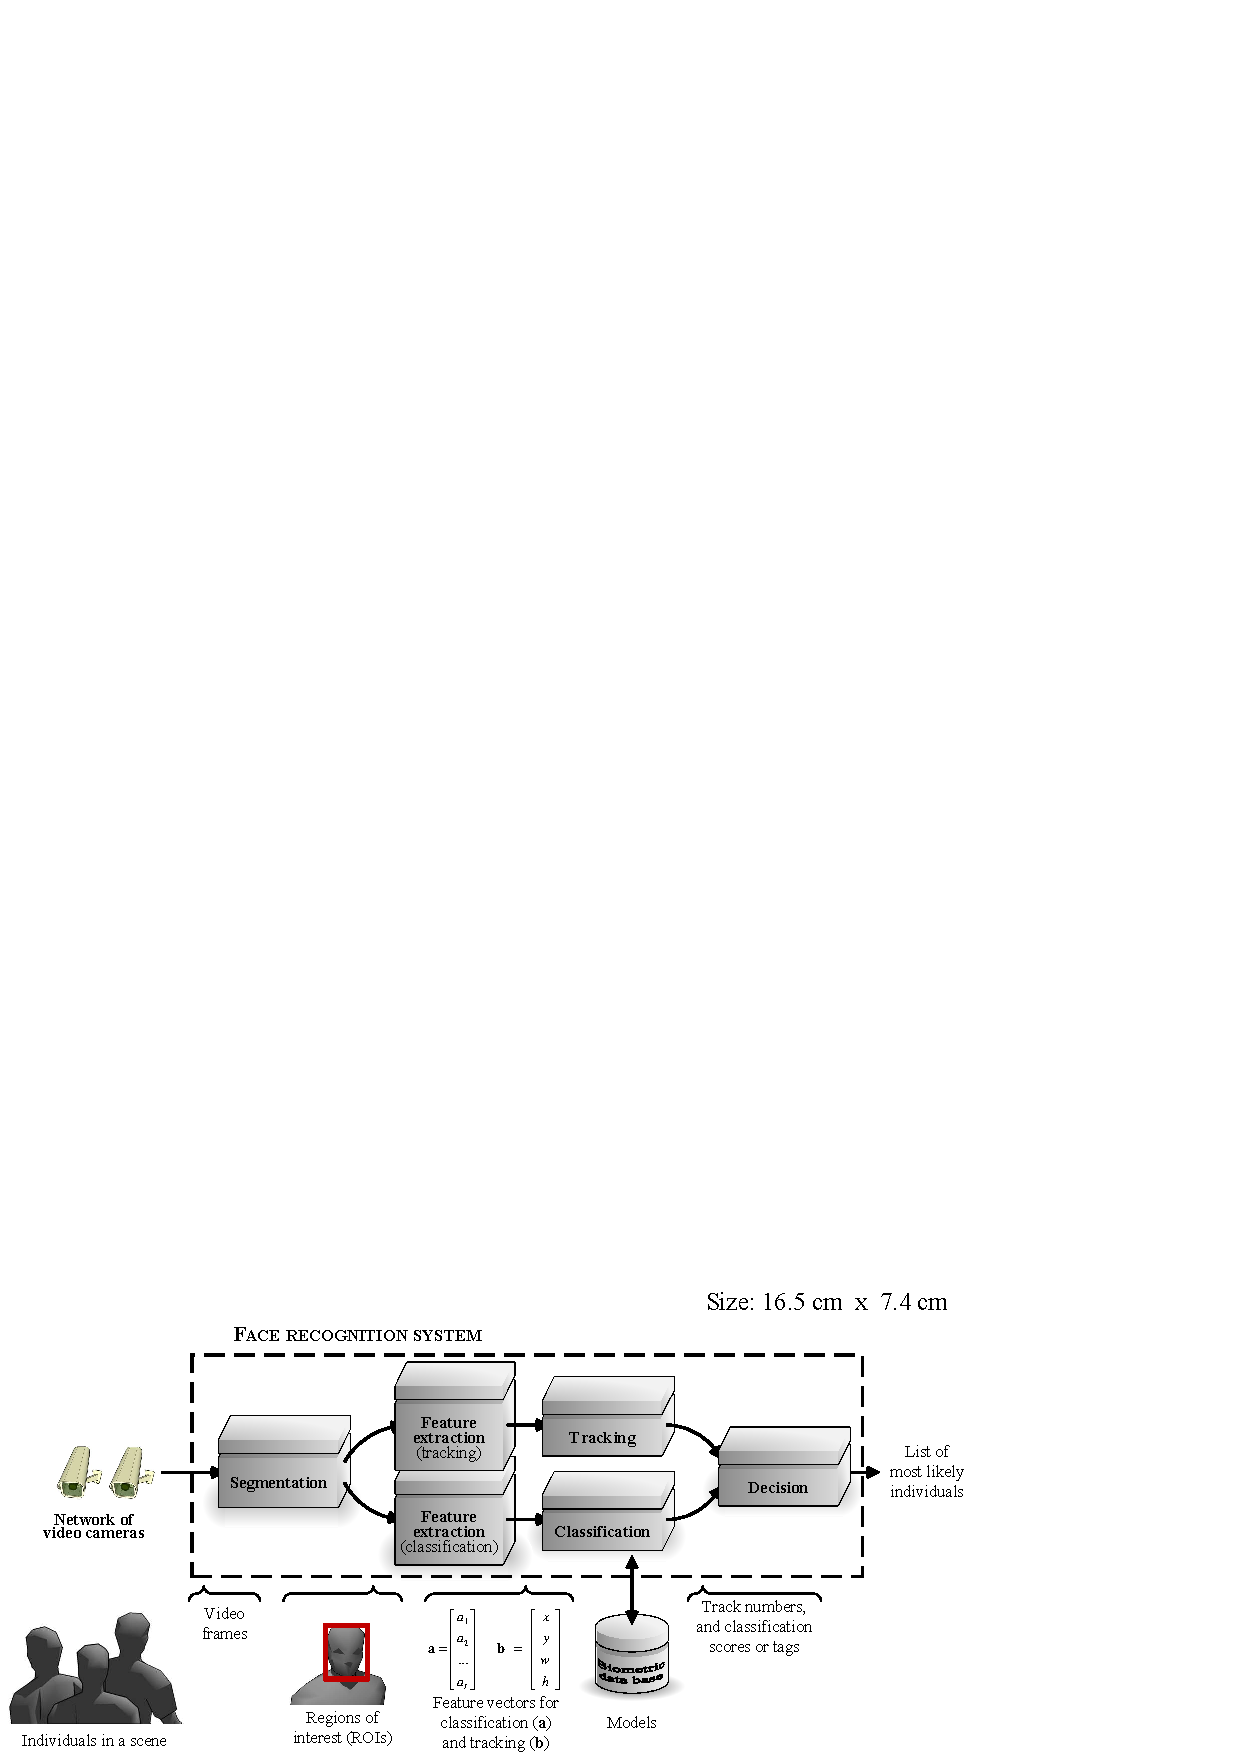
\includegraphics[width =0.97\linewidth, viewport= 0cm 0cm 16.5cm 7.4cm, clip]
 		              {c3_fig2} }
  \caption{A generic track-and-classify biometric system for video-based face recognition}
	\label{fig:c0_faceRec}
\end{figure*}
%-------------------------- /Face recognition system --------------------------%

In this thesis, video-based face recognition is performed with a track-and-classify system that combines the responses of a classifier to kinematic information of individuals and the appearance of faces in a scene (see Figure \ref{fig:c0_faceRec}).
It is assumed that 2D images in the video streams of an external 3D scene are captured using one or more IP or network cameras.
Each camera captures a sequence of 2D images, or frames, from the external scene, and each frame provides the system with a particular view of individuals populating the scene.

First, the system performs segmentation to locate and isolate regions of interest (ROIs) corresponding to the faces in a frame.
In this thesis, the well known Viola-Jones face detection algorithm (\cite{viola01}) is used for this task.
From the ROIs, features are extracted for tracking and classification.
The tracking features can be the position in the 2D images, speed, acceleration, and track number assigned to each ROI on the scene so that the tracking module may follow the movement or expression of faces across the frames.
On the other hand, classifiers will require invariant and discriminating classification features extracted from the ROIs, so that the classification module may match input feature patterns to an individual registered in the system.
Facial matching may be implemented with templates, statistical, or neural pattern classifiers.
Since feature-based methods like Elastic Bunch Graph Matching tend to become complex when several individuals and cameras are involved, the predominant techniques used with this type of architecture are the same appearance-based methods (Eigenfaces, Fisherfaces, etc.) used to represent faces in static 2D images (\cite{zhang09, zhao03}).

The decision module may then combine and accumulate the responses from the tracking and classification modules over several frames (\cite{granger01}).
With identification and surveillance applications for instance, ambiguity is reduced by accumulating responses (classification scores) obtained for each frame over the trajectory of each individual in the scene.

This thesis discusses the use of a video face recognition for closed-set identification, in applications such as access control for security checkpoints or for computer login.
More specifically, it is interested in the process by which facial models of individuals are updated over time with new data in the face recognition system. 
It explores the two most plausible scenarios that can occur in this situation: (1) new individuals are presented one at a time to build the models (enrollment), or (2) individuals already seen by the system are presented, again, one at a time, to update the existing models (re-enrollment).  
It is assumed that new labeled reference data becomes available over multiple (re)enrollment sessions, or when operational scenarios are analyzed off-line, and may belong to new individuals to be registered in the face recognition system.
While the design and update of the class models can be performed off-line, identification, among several individuals registered in the face recognition system, of the ROI(s) in each in a frame must be performed in real time.

%------------------------------ Problem statement -----------------------------%
\section{Problem Statement}

\subsection{Biometric Systems}

%-- Why neural network classifiers
%-- Biometric / face recognition -- lack of data
In biometric applications, including face recognition, matching is typically performed by comparing query samples captured with some sensors against biometric class models (\emph{i.e.}, an individual's facial model) designed with reference samples captured during an enrollment process.
In its most basic form, a biometric model consists of a set of one or more templates (features representing a person's biometric trait) stored in a biometric data base (Figure \ref{fig:c0_faceRec}).
Since reference data is sampled from an unknown probability distribution, biometric class models may also consist of a statistical representation estimated by training a discriminative classifier on these data to improve robustness and reduce resources.
Then, neural or statistical classifiers implicitly define the biometric model of an individual's physiological or behavioral trait with a set of parameters and map the finite set of reference samples defined in an input feature space to a set of predefined class labels in an output space.
The collection and analysis of reference data are often expensive and time consuming because real individuals are involved in the process.
Therefore, classifiers are often designed using some prior knowledge of the underlying data distributions, a set of user-defined hyperparameters (\emph{e.g.}, learning rate), and a limited amount of reference data.

%-- Why adaptation 
In real applications, it is possible to acquire new reference samples at some point in time, after a classifier has originally been trained and deployed for operations.
Labeled and unlabelled reference data can be acquired to update the class models of pre-existing individuals through re-enrollment sessions and analysis of operational data, or enrollment of new individuals in the system.
In addition to changes that may occur when acquiring images from unconstrained scenes, the physiology of individuals may change over time, either temporarily (\emph{e.g.}, haircut, glasses, etc.) or permanently (\emph{e.g.}, scars, aging).
New information such as input features and new individuals may emerge, and previously acquired data may become obsolete in dynamically changing classification environments (\cite{granger01, tsymbal08}).

%-- Adaptive biometric systems - templates
In the literature, specialized adaptive biometric systems have been proposed to define and refine biometric models according to intra-class variations in new reference samples.
These methods focus on procedures to update templates initially designed during enrollment, and perform recognition with a biometric model consisting of one, several, or even a super template (several templates combined to form a single one).
The update procedures either involve semi-supervised learning strategies with highly confident unlabeled data obtained during operations (\cite{poh09, rattani10}), clustering and editing techniques to update selection of user templates from a gallery with labeled reference samples (\cite{uludag04}), or on-line learning of genuine samples over time to update each user's single super template (\cite{jiang02}).
These methods have been showed to be vulnerable to intra-class variations, such as outliers, dispersion and overlap in class distributions.
In all cases, the biometric facial model of an individual tends to diverge from its underlying class distribution due to limited reference data, complexity, and changes in the classification environments.

\subsection{Statistical and Neural Classifiers}

Although using statistical and neural pattern classifiers may represent a flexible solution to a biometric recognition problem, their performance depends heavily on the availability of representative reference data.
Moreover, the majority of the classifiers proposed in the literature assume a static classification environment and can only perform \emph{supervised batch learning} of a finite data set.
To account for new information from new data, they must accumulate it in memory and train from the start using all previously acquired learning data.
Otherwise, new data may corrupt the classifier's previously acquired knowledge, and compromise its ability to achieve a high level of generalization during future operations (catastrophic forgetting problem).
In the context of a face recognition problem, this would lead to the corruption of facial class models when new data are added in time.

Video-based face recognition is becoming an important function in enhanced surveillance systems, which must simultaneously process many video feeds.
As these applications must perform in real-time, the design of efficient systems for facial matching involves a trade-off between classification speed, accuracy, and resources for the storage of facial models.
For instance, today's video surveillance networks are comprised of a growing number of IP cameras.
The need to design and store representative facial models for recognition -- either more user templates or their statistical representation -- increases the resource requirements of the system.
In addition, matching captured facial images to models for a large number of frames from different sources may severely increase the computational burden.
Finally, the memory and time complexity associated with storing and relearning from the start on all cumulative data makes supervised batch learning impossible in this situation. 

%-- Incremental learning
When new data becomes available, classifiers can be updated through \emph{supervised incremental learning} in order to accommodate new knowledge and avoid a growing divergence between class models and their underlying distributions. This method does not involve the redundant and costly computations of batch learning; it rather reduces the memory resources associated with storing classifiers.

Learning and adapting classifiers in changing classification environments raises the so-called stability-plasticity dilemma, where stability refers to retaining existing and relevant knowledge while plasticity enables learning new knowledge (\cite{grossberg88}).
The literature proposes many classifiers which re-estimate their own parameters and architecture through incremental learning (\cite{carpenter91, chakraborty03, fritzke96, okamoto03, ruping01}).
However, if the plasticity of these classifiers is not adjusted to accommodate new knowledge presented with new reference data, they can still be affected by the catastrophic forgetfulness problem (\cite{canuto00, dubrawski97, fung03, granger07, kapp09}).

\subsection{Adaptive Ensembles}

Recently, various methods employing adaptive ensembles of classifiers to perform incremental learning have been put in practice (\cite{polikar01, kapp10}).
For a wide range of applications, where adaptation is not necessarily required, classifier ensembles allow to exploit several views of a same problem to improve the overall accuracy and reliability.
With the use of a combination function, they also offer a flexibility over single classifiers in how class models can be managed and adapted. 
These methods can be divided in three general categories (\cite{kuncheva04}).
Dynamic combination, or ``horse racing'', methods where individual base classifiers are trained in advance to form a fixed ensemble where only the combination rules is changed dynamically (\cite{blum97, widmer96, xingquan04}).
Methods that rely on new data to update the parameters of ensemble base classifiers an online learner (\cite{gama04}).
If blocks of data are available, training can also be performed in batch mode while changing or not the the combination rule at the same time (\cite{breiman99, ganti02, oza01, wang03}).
The last main category consists of methods that grow ensembles by adding new base classifiers and replacing old or underperforming ones when new data is available (\cite{chen01, street01, kolter07, tsymbal08}).
Finally there are adaptive ensembles that use hybrid approaches that combine adding new base classifiers and adjusting the combination rule to update class models.
The most notable are streaming random forests with entropy (\cite{abdulsalam11}), Hoeffding tree with Kalman filter-based active change detection using adaptive sliding window (\cite{bifet10}), maintaining and choosing the better of two ensembles trained with current and old data (\cite{scholz06}), and the AdaBoost-like Learn++ (\cite{polikar01}).

Among these methods, horse racing approaches cannot accommodate new knowledge since base classifiers in the ensemble are never updated with new data.
On the other hand, while online learners and growing ensembles can be used to explore unknown regions of the feature space, most methods focus on the notion of concept drift where underlying class distributions changes in time.
They incrementally append new classifiers to a pool without updating pre-existing members to change their parameters and risk losing old knowledge.
While these classifiers are trained with new data, their plasticity (or learning dynamics) is set beforehand and remains fixed throughout the learning process, without being adjusted to accommodate new knowledge.
Their claim is that old concepts, represented by old data should never be revisited and \emph{reinforced} in contrast with new concept presented with new data.
Although this may happen in a face recognition application, when classes are added and removed from the system for instance, it is not necessarily the case.
In fact, when few biometric reference samples are available, the change that most commonly occurs is the knowledge of the underlying distributions, which is initially incomplete.
Moreover, face recognition systems in unconstrained scenes are often faced with recurring changes regarding the environment (\emph{e.g.}, light effect over the course of a day) and the individuals to recognize (beard, haircut, glasses, etc.).
In this context, adaptive ensemble methods that focus on concept drift may then forget old concepts that are still valid.

As it is detailed with the Learn++ algorithm (\cite{polikar01}) in Appendix \ref{sec:c0_learn++}, methods that rely exclusively on adding new ensemble members to explore the feature space become problematic if all classes are not always represented.
With the current face recognition application for instance, when new data becomes available after a classifier is designed and deployed in the field, it will most likely be sampled from few, or even, one person at a time. 
While previously trained classifiers will not be able to recognize new classes, the ones trained with the new data will contained only the facial models of individuals registered in the system at that time.

%-------------------------- Objectives & contribution -------------------------%
\section{Objective and contributions}

This thesis addresses the challenges mentioned before and seeks to provide a video face recognition system with a mean to perform enrollment and update of biometric models \emph{incrementally} when new data becomes available.
In the context of real-world video applications, where classifier predictions must be accurate and be available in real-time, an ideal face classifier must accommodate emerging reference samples such that  two objectives are minimized: classification error rate and computational cost.
To achieve this, the relationship between a classification environment, where a classifier's decision boundaries are defined, and an optimization environment, comprise of a hyperparameter search space and an objective space, is studied and characterized.
The result, and the core of this thesis, is a supervised incremental learning strategy based on particle swarm optimization (PSO) that is used to evolve a swarm of fuzzy ARTMAP (FAM) neural networks in response to new data.
As each particle in a hyperparameter search space corresponds to a FAM network, the learning strategy co-optimizes all classifier parameters -- hyperparameters, weights, and architecture -- in order to maximize accuracy, while minimizing computational cost and memory resources.

In addition to the incremental learning strategy, this thesis presents the following key contributions.
\begin{itemize}
	%-- Incremental learning properties
	\item The original definition of incremental learning is reconsidered.
The original definition, proposed by (\cite{polikar01}), states a classifier that can perform supervised incremental learning should:
\begin{enumerate}
	\item allow learning of additional information from new data, 
	\item not require access to the previous learning data,
	\item preserve previously acquired knowledge, and
	\item accommodate new classes that may be introduced with the new data.
\end{enumerate}
In order to mitigate corruption of previous knowledge when learning new data, a fifth property is considered: the classifier should also adapt its plasticity by adjusting its hyperparameters for accurate and timely recognition.
Furthermore, the second property is changed so that some previously acquired knowledge is necessary during the incremental learning process.
Otherwise, adaptation is only performed according to new data, and the classifier is subject to the problem of catastrophic forgetfulness.
	%-- Dynamic optimization problem
	\item Adapting FAM's plasticity by adjusting its hyperparameters with a particle swarm optimization (PSO) algorithm during incremental learning in order to maximize accuracy is shown to be a dynamic optimization problem.
More specifically, it is shown to correspond to a type III dynamic optimization problem, where both the location of the optimum on the objective function, as well as its value, change in time.
To properly adapt FAM networks to new data, dynamic particle swarm optimization (DPSO) must be use, otherwise performance decreases during the learning process.  
	%-- Correlation between particle and classifier diversity
	\item It is empirically shown that genotype diversity in the hyperparameter search space is correlated with classifier diversity in the classification environment.
When a pool of FAM classifiers are trained on the same data, the resulting decision boundaries of each FAM network change according the hyperparameter values with which it was trained.
With several correlation and diversity indicators, results then indicate that, as genotype diversity among swarm of particles (\emph{i.e.}, hyperparameter values) increases, diversity among a corresponding  pool of classifiers also increases.
This property allows the diversity of solutions to be easily controlled in the optimization environment.
	%-- Ensemble selection
	\item Following the previous contribution, a greedy search algorithm is presented to perform an efficient selection of diversified ensembles of classifiers among a pool.
Instead of evaluating costly classifier diversity indicators that would involve computing predictions over validation data sets, the greedy search aims to maximize genotype diversity in the search space.
Although this approach does not ensure finding an ensemble with the global optimum particle diversity, this algorithm allows to select ensembles that yield classification rates comparable to that of reference ensemble-based and batch learning techniques, but with only a fraction of the resources.
	%-- Optimization algorithm to perform DMO
	\item An aggregated dynamical niching PSO (ADNPSO) algorithm is presented to guide a swarm of FAM networks according two objectives: FAM accuracy and network size (\emph{i.e.}, computational cost).
Instead of purely solving a multi-objective optimization problem to provide the Pareto-optimal front, ADNPSO is rather aimed at generating pools of classifiers with high genotype and phenotype (\emph{i.e.}, fitness) diversity.
Unlike existing multi-objective optimization (MOO) algorithms (such as NSGA, MOEA, MOPSO, etc.), fitness values and future research directions of each particle do not rely on the notion of dominance in the objective space;
these are defined directly according to the different objective functions.
The ADNPSO algorithm then allows to direct particles toward different local Pareto fronts.
In conjuncture with the latter, a specialized archive is used to categorize solutions according FAM network size and then capture locally non-dominated FAM network.
Creating ensembles of FAM networks with ADNPSO and the specialized archive have shown to provide accuracy comparable to that of using mono-objective optimization, yet requires a fraction of the computational cost.
\end{itemize}

In this thesis, performance of AMCSs is assessed in terms of classification rate and resource requirements for incremental learning of new data blocks from two real-world video data sets -- Institute of Information Technology of the Canadian National Research Council (IIT-NRC) (\cite{gorodnichy05}) and Motion of Body (MoBo) (\cite{gross02}).
For each chapter, the proposed system is compared to other optimization methods to adjust the hyperparameters and ensemble selection methods relevant to the subject at hand.
For all chapters, results are also given for a reference PSO-based batch learning method (\citep{granger07}), \textit{k}NN, and other face recognition systems that were tested on the IIT-NRC and MoBo data bases. 
Since these data bases were treated with Principal Component Analysis, using \textit{k}NN during face recognition may be considered as using eigenfaces.

%-------------------------------- Organization --------------------------------%
\section{Organization of the Thesis}

This manuscript-based thesis is organized into three chapters and two appendixes.
Each chapter consist of published (or submitted for publication) articles in refereed scientific journals.
The content of each chapter is almost the same as that of the papers, with minor modifications for consistency in the notation throughout the thesis. 
While all chapters present a classification system that is used in conjuncture with a supervised incremental learning strategy, they each present a sequential evolution of the classification system in which: 
\begin{enumerate}
	\item only one network is optimized at a time during mono-objective optimization (Chapter 1),
	\item a swarm of networks is optimized, followed by ensemble selection and combination, again during mono-objective optimization (Chapter 2),
	\item optimization of the swarm and ensemble selection is now performed in a multi-objective framework (Chapter 3).
\end{enumerate}
As each chapter can be read independently, an overlap of content between them could not be avoided.


Chapter 1 presents an adaptive classification system (ACS) for video-based face recognition.
It combines a FAM neural network classifier, DPSO algorithm, and a long term memory (LTM).
A DPSO-based learning strategy is also presented for incremental learning of new data with this ACS.
This strategy allows to conjointly optimize the classifier weights, architecture, and user-defined hyperparameters such as accuracy is maximized.
The necessity of a LTM to store validation data is shown empirically for the enrollment and update scenarios.
In addition, incremental learning is shown to constitute a dynamic optimization problem where the optimal hyperparameter values change in time.
While this chapter illustrates the dynamic nature of the problem when all four FAM hyperparameters are optimized, Appendix I presents a two dimensional example of an objective function that changes in time when only the $\beta$ and $\epsilon$ are optimized with a simple grid.

In Chapter 2, a DPSO-based incremental learning strategy is proposed to evolve heterogeneous ensembles of classifiers (where each classifier corresponds to a particle) in response to new reference samples.
Unlike in the previous chapter, this strategy now evolves a swarm of FAM neural networks (instead of only one).
It is applied to an adaptive multiclassifier system (AMCS) that consists of the swarm (or pool) of FAM neural networks and a niching version of DPSO that still optimizes all FAM parameters such that the classification rate is maximized.
Given that diversity within a dynamic particle swarm is correlated with diversity within a corresponding pool of base classifiers, DPSO properties are exploited to generate and evolve diversified pools of FAM classifiers, and to efficiently select ensembles among the pools based on accuracy and particle swarm diversity.

Chapter 3 presents a third version of the incremental learning strategy that now co-optimized all parameters of the swarm of FAM classifiers such that both error rate and computational cost are minimized. 
The AMCS integrates information from multiple and diverse classifiers where learning is guided by an aggregated dynamical niching PSO (ADNPSO) algorithm that optimizes networks according the two objectives.
Pools of FAM networks are now evolved to maintain genotype diversity of solutions around local optima in the optimization search space and phenotype diversity in the objective space.
The AMCS previously presented in Chapter 2 is modified with an archive that stores FAM classifiers on the notion of local Pareto-optimality.
Accurate ensembles with low computational cost are then designed by selecting classifiers on the basis of accuracy, and both genotype and phenotype diversity.

Finally, a summary of the contributions and a discussion for future extensions of this research are presented in the conclusion.

\end{introduction}

%---------------------------------- Chapters ----------------------------------%
\chapter{An adaptive classification system for video-based face recognition}

This chapter presents an initial version of a supervised incremental learning strategy applied to a classification system where the accuracy of only one FAM neural network is maximized every time new data is available.
It is a first step in characterizing the relationship between the classification and optimization environments for a mono-optimization problem.
It was published in the special edition of the Information Sciences journal (Elsevier) on Swarm Intelligence and Applications \cite{connolly10}. 

In this chapter, an adaptive classification system (ACS) is proposed for video-based face recognition. It combines a fuzzy ARTMAP neural network classifier, dynamic particle swarm optimization (DPSO) algorithm, and a long term memory (LTM). A novel DPSO-based learning strategy is also presented for incremental learning of new data with this ACS. This strategy allows to cojointly optimize the classifier weights, architecture, and user-defined hyperparameters such as classification rate is maximized. Performance of this system is assessed in terms of classification rate and resource requirements for incremental learning of data blocks coming from real-world video data bases. The necessity of a LTM to store validation data is shown empirically for different enrollment and update scenarios. In addition, incremental learning is shown to constitute a dynamic optimization problem where the optimal hyperparameter values change in time. Simulation results indicate that the proposed system can provide a significant higher classification rate than that of fuzzy ARTMAP alone during incremental learning. However, optimization of ACS parameters requires more resources. The ACS needs several training sequences to produce the optimal solution, and adapting fuzzy ARTMAP parameters according to classification rate tends to require more category neurons and training epochs.

%-------------------------------- Introduction --------------------------------%
\section{Introduction}

Biometric systems seek to recognize individuals from their behavioral or physiological characteristics such as the face, finger print, iris, signature and voice (\cite{jain06}). Since these characteristics are unique for each individual, and cannot be lost, stolen or reproduced, as with current approaches (\emph{e.g.}, passwords, access cards and identification numbers and cards), they can be used to prevent theft and fraud. There are three types of applications in biometric recognition -- verification, identification, and surveillance (\cite{jain06}). In verification applications, an individual enrolled in the system identifies himself and provides a biometric sample. Then, the biometric system seeks to authenticate that the sample corresponds to the model of that specific individual. In contrast, in identification applications, an individual provides a biometric sample, and the system seeks to determine if the sample corresponds to the model of any of the individuals enrolled to the system. Surveillance applications differ slightly from identification in that the sampling process is performed discretely in an \emph{unconstrained} scene, and it seeks to determine if a given biometric sample corresponds to the model of a restrained list of individuals under surveillance, \emph{e.g.}, screening for criminals or terrorists in an airport setting.

Over the past decade, face recognition has received considerable attention in the area of biometrics due to the wide range of commercial and law enforcement applications, and to the availability of affordable technologies. \emph{Video-based} face recognition has the advantage other very reliable characteristics for biometric recognition, such as iris and fingerprint scans, that it does not require the cooperation of individuals involved in the process (\cite{zhao03}). It can thus be used for surveillance applications where control of the acquisition conditions are not possible. In addition, unlike applications of \emph{image-based} face recognition, it is possible to recognize targeted subjects from a sequence of video frames, instead of only one image. As outlined in the following, video-based face recognition for surveillance applications remains a very challenging problem.

A critical function in face recognition systems is the classification of face regions captured in video streams. Typically, face recognition systems employ statistical or neural pattern classifiers to map an $\mathbb{R}^I$ input feature space to a set of K predefined class labels $\Omega = \left\{C_1, C_2, ..., C_K\right\}$, where each class $k$ $(k=1,...,K)$ corresponds to the face model of an individual enrolled in the biometric system. From the classifier's perspective, an input pattern $\textbf{a}$ associated with class $k$ is sampled from an unknown probability distribution, $p_k(\textbf{a})$, over the input feature space $\mathbb{R}^I$. In practical applications, the classifiers are designed a priori, using some prior knowledge of the underlying distributions $p_k(\textbf{a})$, a set of user-defined \emph{hyperparameters} (\emph{e.g.}, learning parameter), and a limited amount of learning data.

Since the acquisition (collection and analysis) of such data is expensive and time consuming in many practical applications, it may therefore be incomplete in one of several ways. In \emph{static classification environments}, where $p_k(\textbf{a})$ remain fixed over time, these include a limited number of learning samples, missing components of the input observations, missing class labels during learning, and unfamiliar classes (not present in the learning data set) (\cite{granger01}). Moreover, in video-surveillance applications, learning samples acquired from video streams of \emph{unconstrained} scenes are generally of poor quality with low resolution. They are also subject to considerable variations due to limited control over operational conditions (\emph{e.g.}, illumination, pose, facial expression, orientation and occlusion). These challenges translate to very complex class distributions $p_k(\textbf{a})$, mainly due to inter and intraclass variability. In addition to previously mentioned challenges, an individual's physiology may change over time, either temporarily (\emph{e.g.}, haircut, glasses, etc.) or permanently (\emph{e.g.}, ageing). In the $\mathbb{R}^I$ space, new informations, such as input features and output classes, may suddenly emerge, and previously acquired data may eventually become obsolete in dynamic classification environments, where class distributions $p_k(\textbf{a},t)$ vary or drift in time (\cite{granger01, tsymbal08, widmer96}). The overall result is a divergence between the biometric models learned by a classifier and the underlying distributions $p_k(\textbf{a},t)$ which may significantly degrade performance.

Although learning data is limited, it is common to acquire new data at some point in time after the classifier has originally been trained and deployed for operations. In particular, adaptation of video-based face recognition systems is required during enrollment (new classes are added to the system) and during update (pre-existing classes are refined using the new data). To avoid a growing divergence with the underlying class distributions $p_k(\textbf{a},t)$, the system should then efficiently adapt its face models as new learning data and knowledge becomes available.

The majority of statistical and neural pattern classifiers proposed in literature perform \emph{supervised batch learning} of a finite data set, and assume a static classification environment. To account for new data, they must accumulate all cumulative data in memory and train from the start using all previously acquired learning data. Otherwise, new data may corrupt the classifier's previously acquired knowledge, and compromise its ability to achieve a high level of generalization during future operations. The memory and time complexity associated with storing and relearning from the start on all cumulative data is not feasible for several practical applications. Assuming that new learning data is available, a classifier that allows for \emph{supervised incremental learning} should (1) allow learning of additional information from new data, (2) not require access to the previous learning data, (3) preserve previously acquired knowledge,\footnote{The problem of learning new information incrementally, yet preserving knowledge is referred to as the \emph{stability-plasticity dilemma} (\cite{carpenter87}).} and (4) accommodate new classes that may be introduced with the new data (\cite{polikar01}). Some classifiers proposed in literature are inherently able to perform supervised incremental learning: the Growing Self-Organizing Networks (\cite{fritzke96}) and the ARTMAP Networks (\cite{carpenter91}). Other well known neural networks (MLP, SVM, and RBF) have also been modified to perform such learning (\cite{chakraborty03, okamoto03, ruping01}). In response to new learning data, these classifiers adapt their parameters (\emph{e.g.}, synaptic weights for a neural network) and architecture according to these four incremental learning properties.

In order to mitigate corruption of previous knowledge when learning new data (3$^\mathbf{rd}$ property), a 5$^\mathbf{th}$ property should be considered for incremental learning -- the classifier should (5) adapt its learning dynamics by adjusting its hyperparameters for accurate and timely recognition. In an unconstrained scene and dynamic classification environment, changes in the feature space are likely to occur over time, and re-adjustment of the classifier hyperparameters are needed. Incremental learning is then defined as a \emph{dynamic optimization problem} in the hyperparameters space. Furthermore, the authors have shown in \cite{connolly09} that, unlike the 2$^\mathbf{nd}$ property stated, it is necessary to preserve some learning data for the validation process and fitness estimation. If not, adaptation is only performed according to new data, and the classifier is subject to the problem of catastrophic forgetting.

In this chapter, an adaptive classification system (ACS) is proposed for video-based face recognition. It combines a fuzzy ARTMAP neural network classifier suitable for incremental learning (\cite{carpenter92}), and a dynamic particle swarm optimization (DPSO) algorithm capable of finding and tracking several local optima in the optimization space (\cite{nickabadi08_2}). This system also features a long term memory (LTM) used to store and manage a set of data for cross-validation and unbiased estimation of classification rate. A novel DPSO-based learning strategy is also proposed for incremental learning of new data with this ACS. When new data becomes available, this strategy allows to cojointly optimize the classifier weights, architecture, and user-defined hyperparameters such as classification rate is maximized.

This study focuses on video-based face recognition applications in which two incremental learning scenarios may occur -- enrollment and update. Performance of this system is assessed in terms of classification rate and resource requirements for incremental learning of new data blocks from two real-world video data sets -- IIT-NRC (\cite{gorodnichy05}) and Motion of Body (MoBo) (\cite{gross02}). First, the necessity of storing validation data in LTM is observed empirically by comparing the performances of fuzzy ARTMAP network trained (1) by using standard hyperparameter values, and (2) by optimizing hyperparameters on each new data block, in both cases, with and without LTM. Second, dynamic changes in the fuzzy ARTMAP hyperparameters space are shown to occur in both scenarios during incremental learning. Performance is compared for fuzzy ARTMAP networks trained by optimizing hyperparameters on all new data blocks with (1) dynamic optimization, (2) static optimization, (3) canonical particle swarm optimization, and (4) only on the first data block.

In the next section, a general biometric system for face recognition system is presented. Then, in Section \ref{sec:c1_adaptation}, a description of the adaptive classification system is presented, along with the long term memory used to store and manage validation data, the fuzzy ARTMAP neural network used for classification, and the DPSO algorithm used to optimize its hyperparameters. Then, the data bases, incremental learning scenarios, performance measures and the protocol used for proof-of-concept simulations are described in Section \ref{sec:c1_methodology}. Finally, experimental results are presented and discussed in Section \ref{sec:c1_results_discussion}.

%------------------------------------------------------------------------------%
%------- SECTION - Biometrics and face recognition from video sequences -------%
\section{Biometrics and face recognition from video sequences}
\label{sec:c1_application}

The adaptive classification system proposed in this chapter is applied to the recognition of faces in video streams of a video-surveillance application and replaces the classification module and biometric data base of Figure \ref{fig:c1_faceRec}. However, it can also be employed to a wide range of real-world pattern recognition applications in which complex and changing environments are modeled using neural and statistical classifiers, but where learning data is limited. In face recognition applications, it is assumed that these systems capture a sequence of 2D images or video frames from the \emph{real environment} (external 3D scene) via one fixed camera. Each frame provides the system with a particular view of individuals occupying the scene. First, the system performs segmentation on each frame to locate and isolate regions of interest (ROIs) corresponding to the faces in a frame. Invariant and discriminant features are then extracted from the ROIs and mapped to $\mathbb{R}^I$ feature space. Those feature patterns are employed for classification. That is, feature patterns are matched to the face model of individuals enrolled to the biometric system. Finally, classification scores are used to provide application-specific decisions. For verification applications, the decision module accepts or rejects the authenticity, and for identification and surveillance applications, it outputs a list of the most likely or of all possible matching identities, respectively.

A typical approach to recognizing faces in video consist in applying techniques developed for static 2D images on high quality ROIs produced through face segmentation. Several powerful techniques proposed to recognize faces in static 2D images are described in \cite{zhang09, zhao03}. However, the performance of these techniques may degrade considerably when applied in unconstrained scenes.

%--------------------------- Face recogniton system ---------------------------%
\begin{figure*}[!t]
	\centering
	\fbox{  
  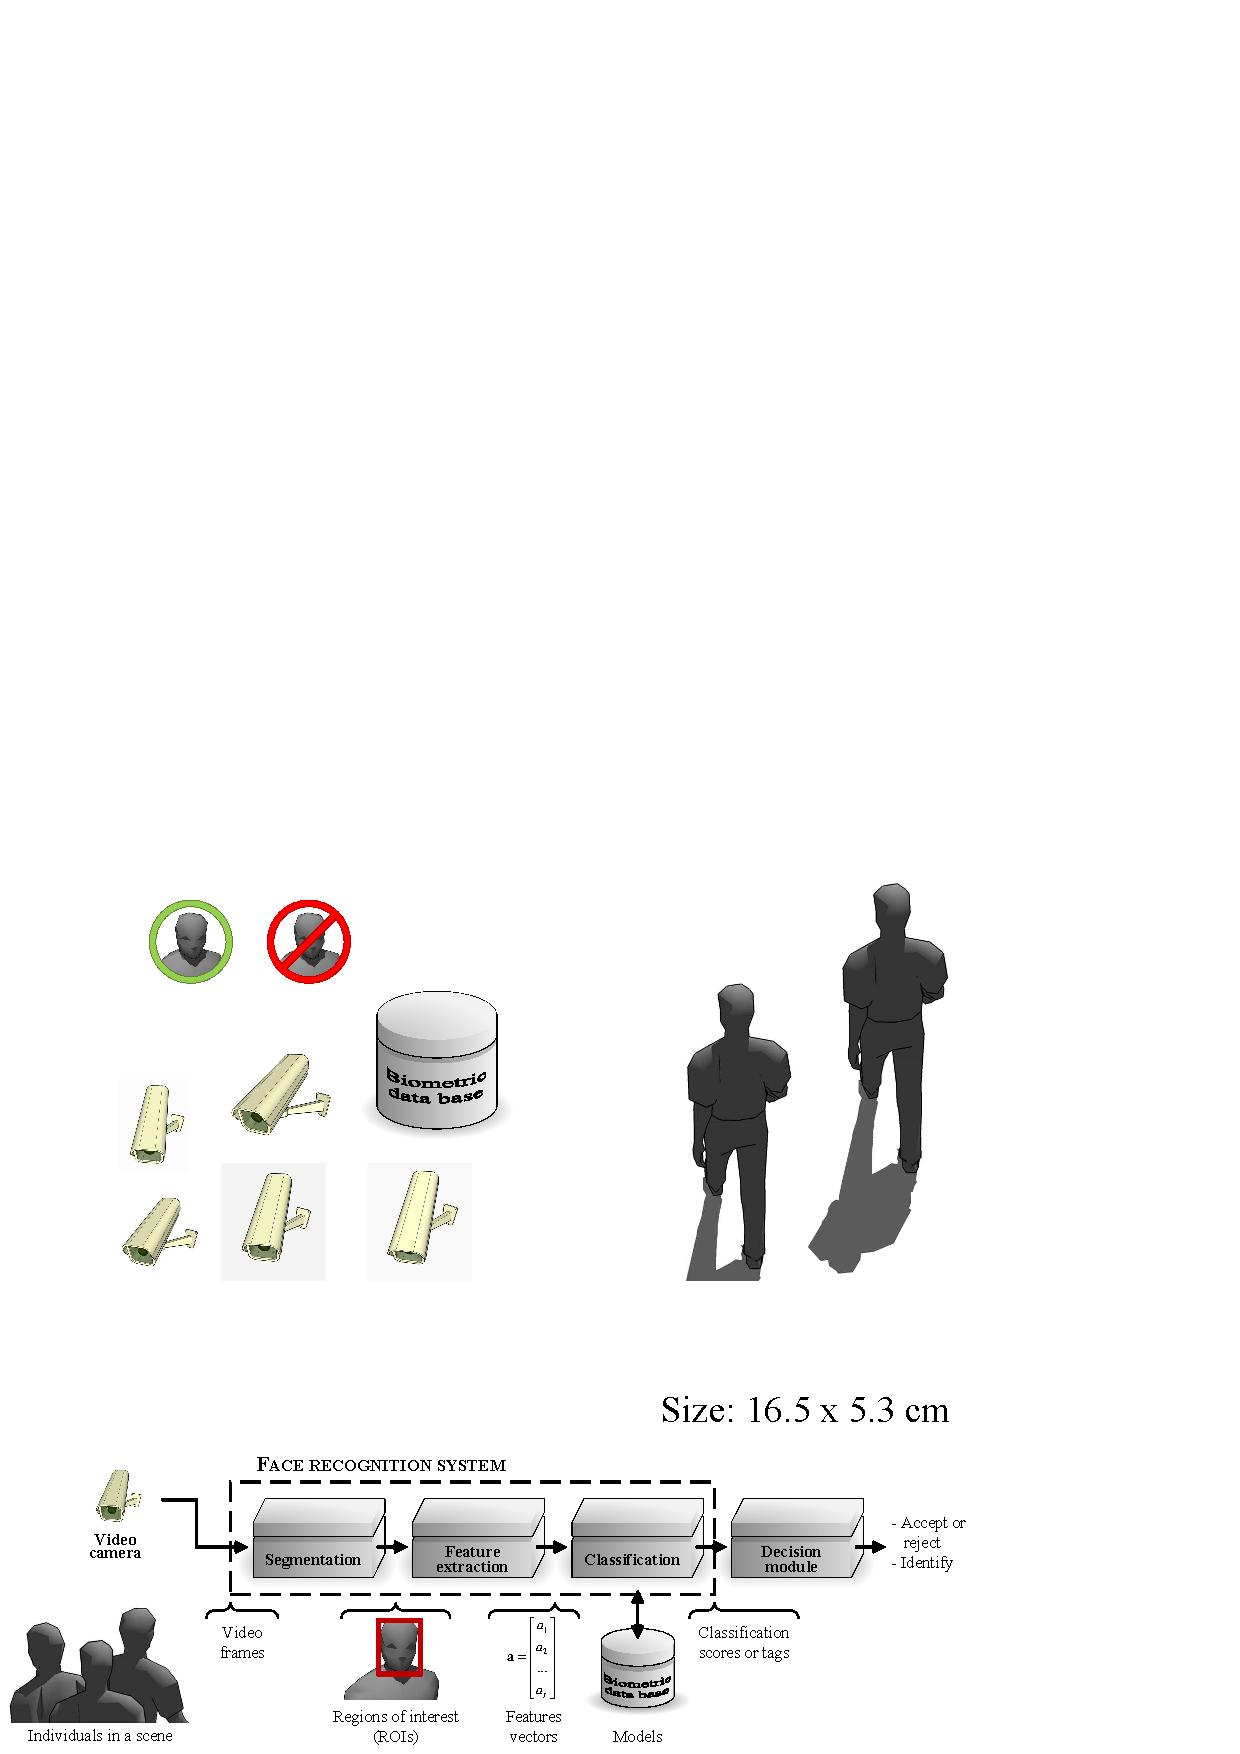
\includegraphics[width=0.97\linewidth, viewport= 0cm 0cm 16.5cm 5.3cm, clip]
 		              {c1_fig1}	}
  \caption{A general biometric system for face recognition. In this chapter, both classification module and biometric data base are replaced by the adaptive classification system}
	\label{fig:c1_faceRec}
\end{figure*}
%-------------------------- /Face recogniton system ---------------------------%

More recently, some authors have combined spatial and temporal information contained in video sequences to provide a higher level of accuracy in unconstrained scenes (\cite{matta09}). These track-and-classify systems combine the responses of a classifier to kinematic information of individuals and faces in a scene. For instance, a distributed sensor network is proposed by \cite{foresti02} as a solution to the problem of partial occlusion that occurs in dynamics environments. \cite{li01} have introduced a face verification system which exploits the trajectories of Gabor facial features to identify individuals through hypothesis testing, using a posterior density characterized by the motion. A time series states space has been proposed by \cite{zhou03} to fuse temporal information in video, which simultaneously characterizes the kinematics and identity of individuals in a probabilistic framework. \cite{barry07} have applied the What-and-Where Fusion neural network to the identification of individuals. This network simultaneously tracks multiple faces in an environment and accumulates their classifier predictions over time to improve classification. \cite{matta07} uses a multimodal system integrating the displacement signals of the head and physiological information with a probabilistic extension of the Eigenface approach. \cite{majumdar08} proposed an image-to-image-based recognition approach that uses color information and a kernel classifier for face authentication. Finally, \cite{mian08} uses an unsupervised learning approach to determine the identity of an individual on the basis of best temporally cohesive matches between clusters of video sequence.

With these systems, the underlying data distribution $p(\textbf{a})$ is considered static in nature and learning occurs only once, during a preliminary design phase. As discussed, once the face recognition system is deployed, temporary and permanent changes may occur in complex real-world environments and the initial learning data may no longer be representative nor sufficient to properly define the underlying class probability distributions $p_k(\textbf{a})$. This may lead to significant degradation in performance during operations. Assuming that new data becomes available, classifiers found in most face recognitions systems in literature would require relearning from the start using all previously acquired data through supervised batch learning. Performing incremental learning with only the new data would therefore be an undisputed asset as the memory and time complexity associated with storing and training is greatly reduced. In addition, it can maintain a high level of performance by reducing the divergence between class models and underlying distributions.

%--------------------------------- Adaptation ---------------------------------%
\section{Adaptive classification system}
\label{sec:c1_adaptation}

Figure \ref{fig:c1_framework} depicts the evolution of the adaptive classification system (ACS) proposed in this chapter for supervised incremental learning of new data. This novel system is composed of a pattern classifier that is suitable for supervised incremental learning, a dynamic optimization module that tunes the user-defined hyperparameters of the classifier, and a long term memory (LTM) that manages and stores incoming learning data used for validation and fitness evaluation.

When a new block of learning data $D_t$ becomes available to the system at a discrete time $t$, part of the data is employed to train the incremental classifier and update the LTM. The classifier then interacts with the dynamic optimization module using a DPSO-based algorithm that cojointly optimizes the vector of user-defined hyperparameters $\textbf{h}$, parameters, and architecture such that classification rate maximized. In this chapter, the fuzzy ARTMAP neural network (\cite{carpenter92}) is employed as an incremental learning classifier and a dynamic version the particle swarm optimization (PSO) algorithm (\cite{kennedy95}) is used for optimization.


%------------------------- Framework - for section 2 --------------------------%
\begin{figure*}[t]
  \centering
	\fbox{
  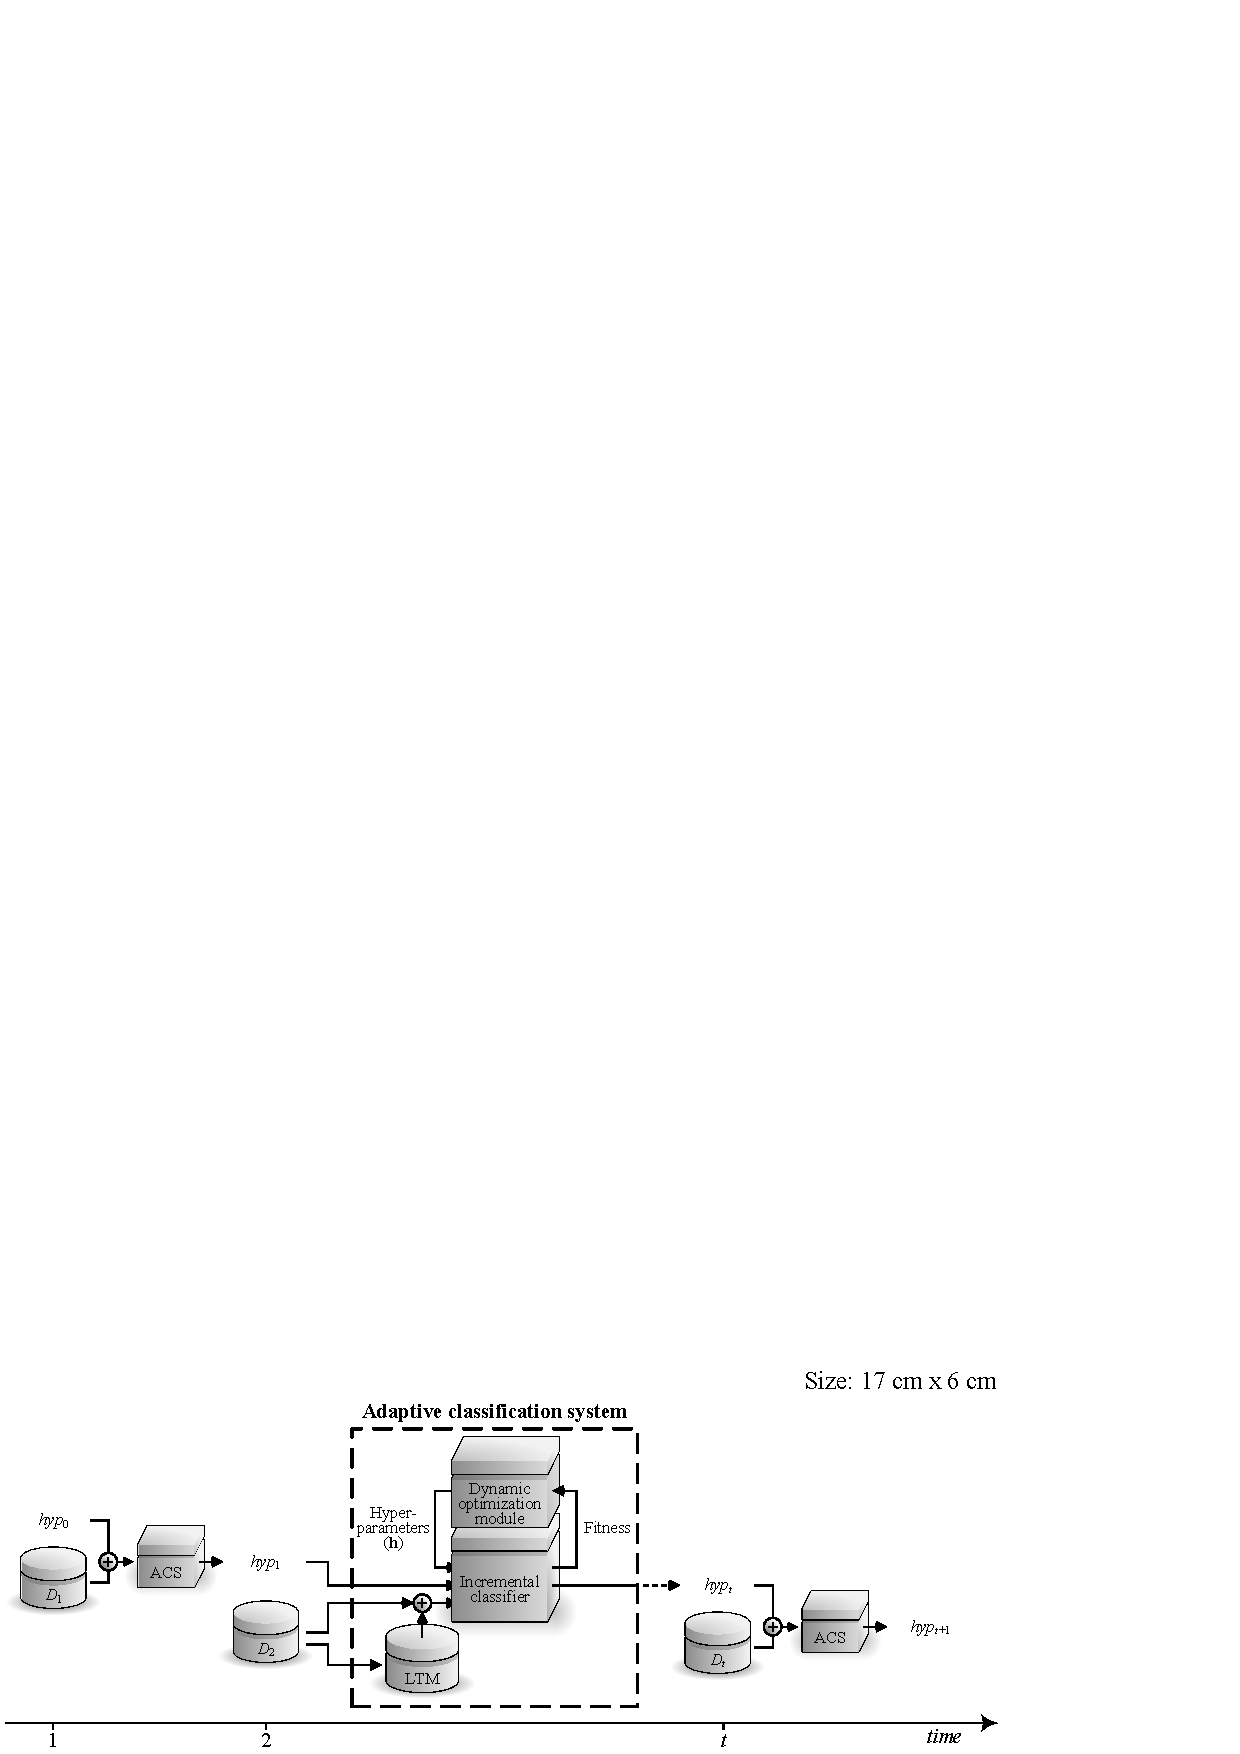
\includegraphics[width=0.97\linewidth, viewport =0cm 0cm 17cm 6cm, clip]
  								{c1_fig2} }
  \caption{The evolution of a new adaptive classification system (ACS) according to generic incremental learning scenario. New blocks of data are used by the ACS to update the classifier over time. Let $D_1$, $D_2$, … be blocks of learning data available at different instants in time. The ACS starts with an initial hypothesis $hyp_0$ which constitutes the prior knowledge of the domain. Each hypothesis $hyp_{t-1}$ are updated to $hyp_t$ by the ACS on the basis of the new data block $D_t$}
	\label{fig:c1_framework}
\end{figure*}
%------------------------------------------------------------------------------%

Most techniques used to optimize fuzzy ARTMAP hyperparameters found in literature allow the optimization of only one or two hyperparameters, even though there are four inter-dependent parameters (\cite{canuto00, dubrawski97, fung03}). In previous work, the authors have introduced a PSO-based learning strategy for mono-objective optimization of all four hyperparameters (\cite{granger07}). It is based on the concept of neural network evolution in that it determines the optimal vector hyperparameters and network weights and architecture such that classification rate is maximized. The PSO strategy has been shown to provide a significantly higher classification rate on several synthetic and real-world data sets (\cite{barry07, granger07}).

While a key feature of ARTMAP networks is their ability to learn new information incrementally, without catastrophic forgetting, those optimization methods have all been developed for batch supervised learning of a finite data set The adjustment of fuzzy ARTMAP hyperparameter vector\footnote{Let $\textbf{h}$ be a vector of user-defined hyperparameters that set classifier dynamics. For fuzzy ARTMAP, it is composed of the four hyperparameters $\textbf{h}=(\alpha, \beta, \epsilon, \bar{\rho})$ described in Section \ref{sec:c1_fam}.} $\textbf{h}$ is then defined as the static optimization problem such that:
\begin{equation}
	\textnormal{maximize }\left\{ f(\textbf{h})\ |\ \textbf{h} \in \mathbb{R}^4 \right\},
	\label{eq:c1_optSta}
\end{equation}
where the objective function $f(\textbf{h})$ is the classification rate. In contrast, the ACS proposed in Figure \ref{fig:c1_framework} performs incremental learning. As shown in Appendix \ref{sec:c1_2Dresult}, incremental learning of new data from the class probability distributions $p_k(\textbf{a},t)$ translates to an objective function $f(\textbf{h})$ that also changes in time. Adapting fuzzy ARTMAP hyperparameters vector \textbf{h} during incremental learning of data blocks $D_t$ to maximize classification rate can thus be formulated as a dynamic optimization problem such as:
\begin{equation}
	\textnormal{maximize }\left\{ f(\textbf{h},t)\ |\ \textbf{h}\in\mathbb{R}^4,
															 t\in\mathbb{N}_1, \right\}
	\label{eq:c1_optDyn}
\end{equation}
where $f(\textbf{h},t)$ is the classification rate of fuzzy ARTMAP for a given vector of hyperparameters h, after learning data set $D_t$ and at a discreet time $t$.

For an optimization space defined by fuzzy ARTMAP hyperparameters, three different types of dynamic optimization environment are then possible (\cite{engelbrecht05}):
\begin{itemize}
	\item \emph{type I environments} where the location of the optimum changes over time,
	\item \emph{type II environments} where the location of the optimum remains fixed, but the value of the objective function at the position of the optimum changes, and
	\item \emph{Type III environments} where both the location and the value of
				optima points change.
\end{itemize}
As results presented in Appendix \ref{sec:c1_2Dresult} suggest the presence of a type III optimization environment for fuzzy ARTMAP hyperparameters adjustment during incremental learning. The ACS employs a DPSO algorithm called Dynamic Niching PSO designed for such environments (\cite{nickabadi08_2}). The rest of this section provides additional details on each part of the adaptive classification system: the long term memory, the fuzzy ARTMAP neural network, and the DPSO-based learning strategy.

%------------------------ Subsection : Long term memory -----------------------%
\subsection{Long term memory}
\label{sec:c1_LTM}

During incremental learning, each new learning block of data $D_t$ is divided into $D_t^\text{t}$ and $D_t^\text{v}$ for training with validation over several training epochs,\footnote{An epoch is defined as one complete presentation of all the patterns of a finite training data set.} and into $D_t^\text{f}$ for estimation of the fitness on the objective function $f(\textbf{h},t)$.

%------------------------------ Data organization -----------------------------%
\begin{figure*}[t]
  \centering
	\fbox{
 	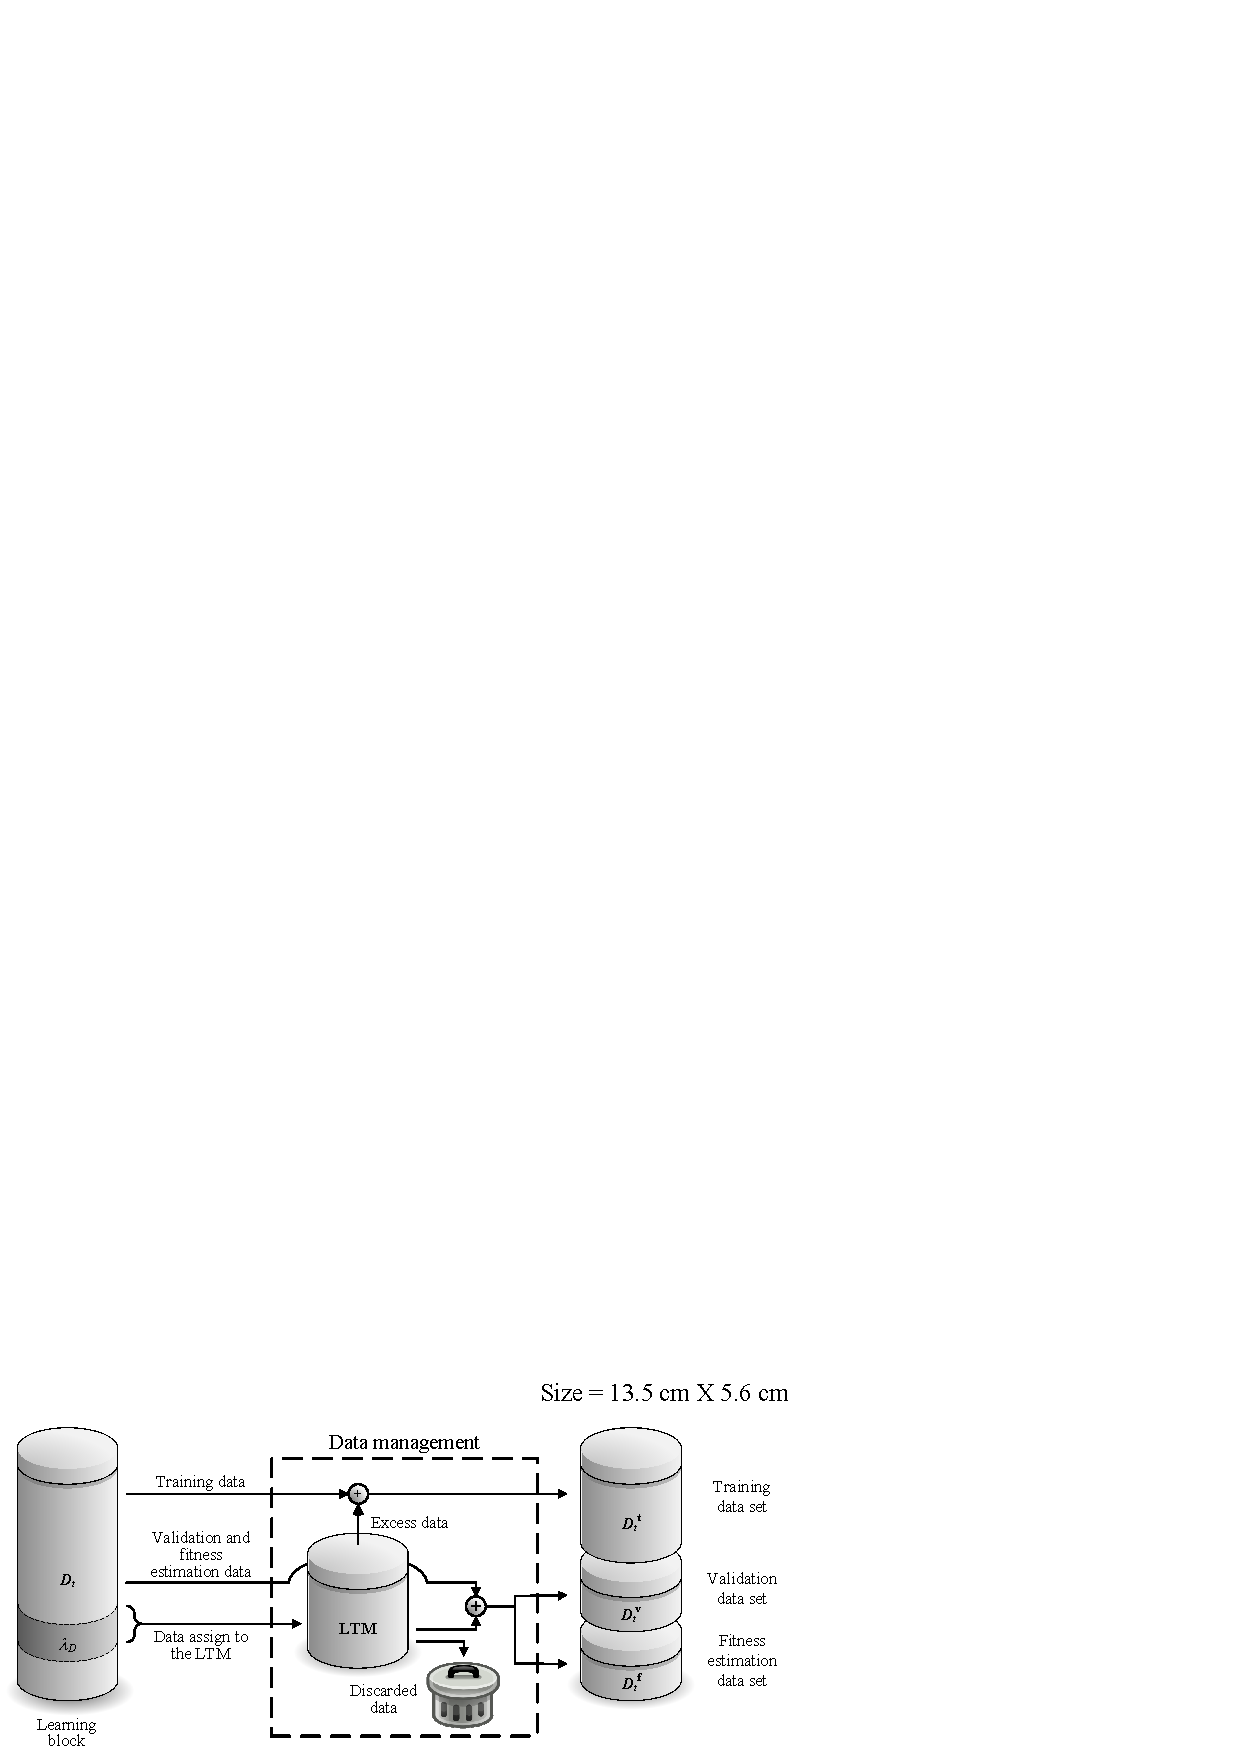
\includegraphics[width=0.97\linewidth, viewport= 0cm 0cm 13.5cm 5.6cm, clip]
								  {c1_fig3}
	}
  \caption{Data management for the learning process using the long term memory. When a learning block $D_t$ is available, a proportion $\lambda_D$ of this data is assigned to the long term memory, and the rest is used for training, validation, and performance estimation. When the LTM is updated, old data is discarded, while excess data not used to fill and/or update the LTM (dues to size limitations) is integrated to the training data from $D_t$ to create the training data set $D_t^\text{t}$. Data contained in the LTM is then combined with data coming directly from $D_t$ dedicated to validation and fitness estimation. This combination is class-wise divided in two, to create the validation data set $D_t^\text{v}$ and the fitness estimation data set $D_t^\text{f}$}
 	\label{fig:c1_LTM}
\end{figure*}
%----------------------------- /Data organization -----------------------------%

It has been shown in \cite{connolly09}, that the data sets used to guide the particles in the optimization space during a PSO-based incremental learning algorithm ($D_t^\text{f}$) should contain a representative set of samples from all classes $C_k \in \Omega$ to avoid a decline in fuzzy ARTMAP performance. As Figure \ref{fig:c1_LTM} depicts, some of the data of each learning block is used to create and maintain a long term memory (LTM). The LTM functions according to two parameters: (1) the proportion of $D_t$ used to fill and update the external data base, $\lambda_D$, and (2) the maximal number of patterns per class in the external data base $|C_k|_\mathbf{LTM}$. Each time a new $D_t$ is presented to the network a proportion $\lambda_D$ of $D_t$ is randomly selected and transferred to the LTM for either addition or update. The LTM is managed as a FIFO (first in, first out) data structure, and the outdated data that surpasses $|C_k|_\mathbf{LTM}$ is discarded. For each class, if the number of patterns transferred exceeds $|C_k|_\mathbf{LTM}$, the excess samples are randomly selected and integrated to $D_t^\text{t}$.

%------------------------- Subsection : fuzzy ARTMAP --------------------------%
\subsection{Fuzzy ARTMAP Neural Networks}
\label{sec:c1_fam}

ARTMAP refers to a family of self-organizing neural network architectures that is capable of fast, stable, on-line, unsupervised or supervised, incremental learning, classification, and prediction (\cite{carpenter91}). A key feature of ARTMAP networks is their unique solution to the stability-plasticity dilemma. They can adjusts previously learned categories in response to familiar inputs, and creates new categories dynamically in response to inputs different enough from those previously seen.

Several ARTMAP networks have been proposed in order to improve the performance of these architectures. They can be broadly divided according to their internal matching process, which depends on either deterministic or probabilistic category activation. The deterministic type consists of networks such as fuzzy ARTMAP, ART-EMAP, ARTMAP-IC, default ARTMAP, simplified ARTMAP, distributed ARTMAP, etc., and represent each class using one or more category hyper-rectangles. In contrast, the probabilistic type consists of networks such as PROBART, PFAM, MLANS, Gaussian ARTMAP, ellipsoid ARTMAP, boosted ARTMAP, $\mu$ARTMAP, etc., and represent each class using one or more probability density functions.

The fuzzy ARTMAP integrates the fuzzy ART to process both analog and binary-valued input patterns to the original ARTMAP architecture (\cite{carpenter92}). This simple and popular neural network has been designed with the ability to perform supervised incremental learning as defined in \cite{polikar01}. In supervised learning mode, the sequential learning process grows the number of recognition categories according to a problem's complexity. The vigilance and match tracking process provide the mechanisms to control the local impact of new data on the existing knowledge structure. Even if fuzzy ARTMAP is able to perform well with few training data (\cite{hennegis06}), previous research by the authors has revealed that the average classification rate of an ARTMAP network trained through incremental learning is usually significantly lower than if trained on all the data through batch learning (\cite{granger08, connolly08}).

%-------------------------------- Fuzzy ARTMAP --------------------------------%
\begin{figure}[!t]
  \centering
	\fbox{
  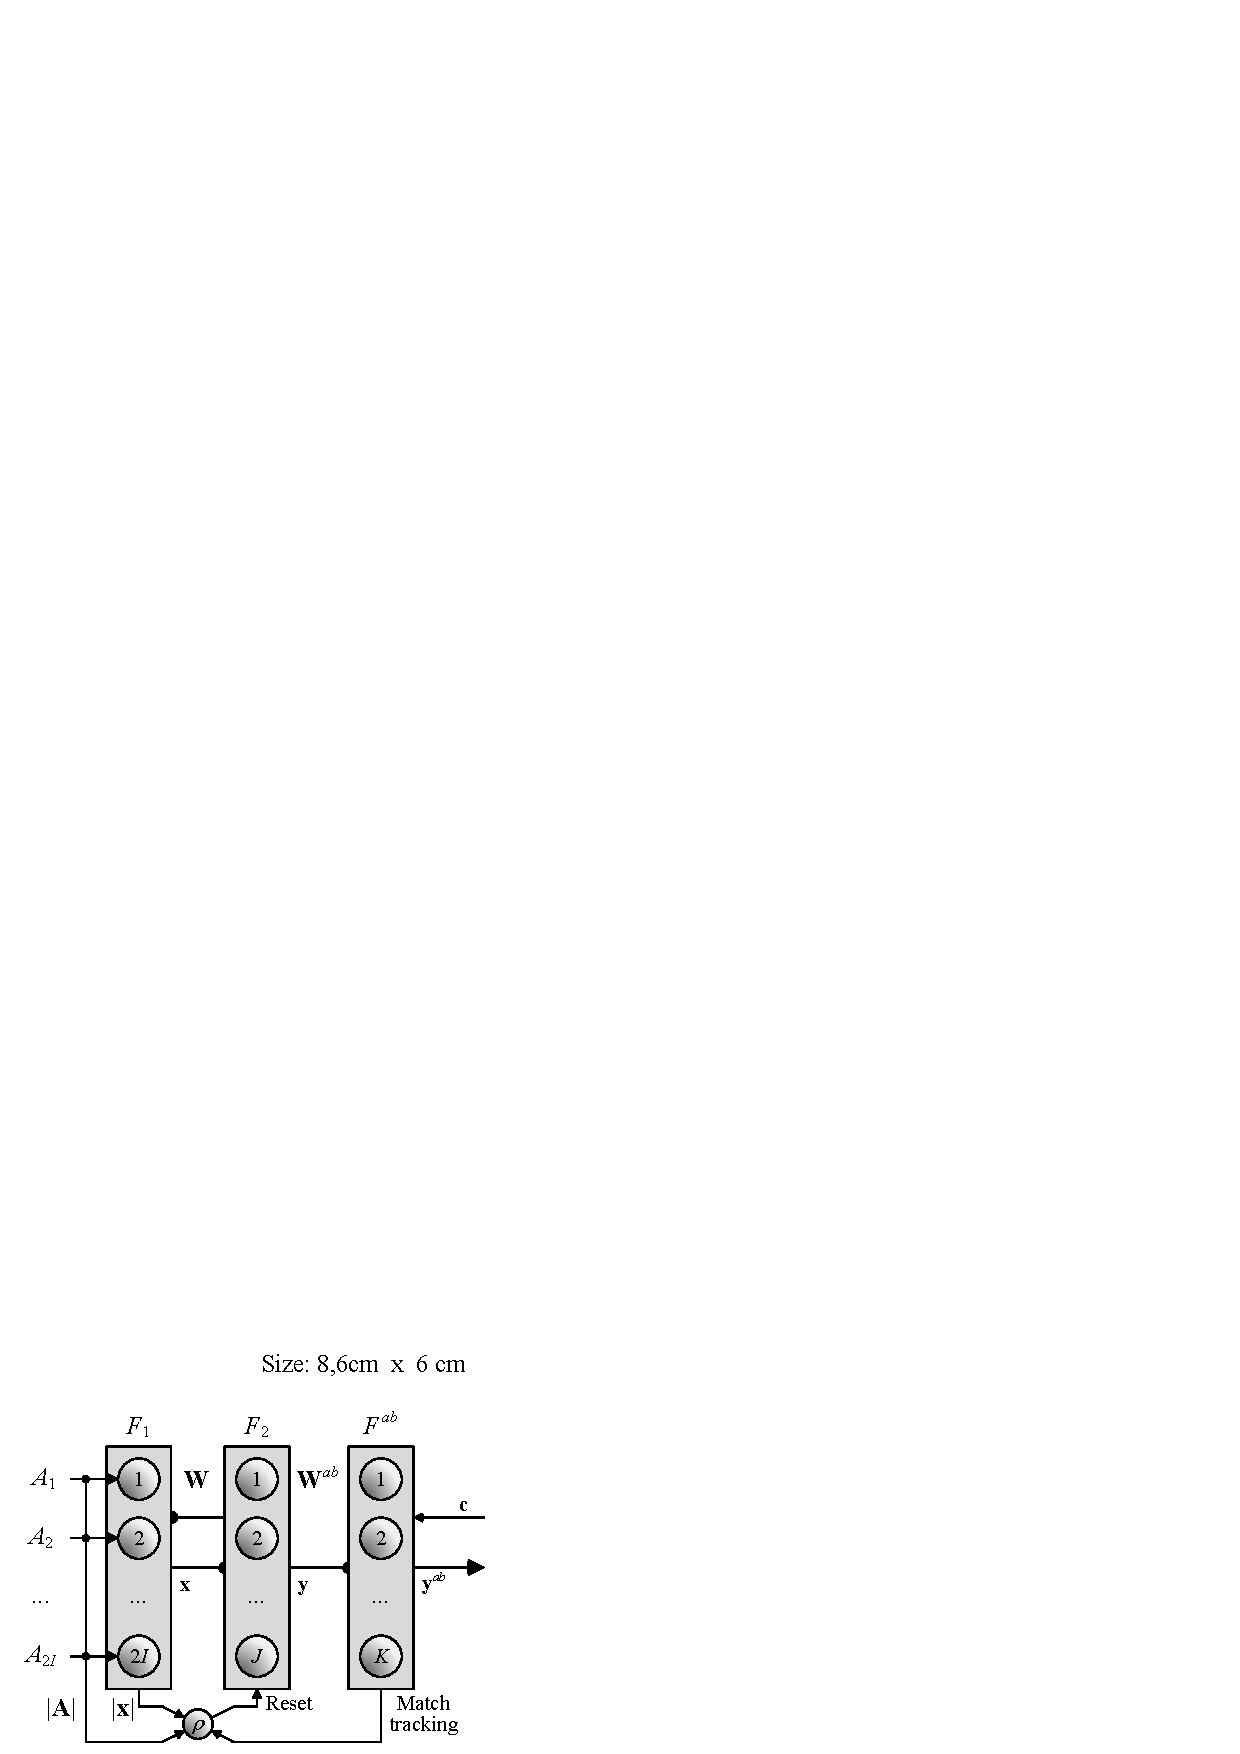
\includegraphics[width=0.5\linewidth, viewport=0cm 0cm 8.6cm 6cm, clip]{c1_fig4}
	}
  \caption{Fuzzy ARTMAP neural network}
	\label{fig:c1_fam}
\end{figure}
%------------------------------------------------------------------------------%

Fuzzy ARTMAP consists of three layers (Figure \ref{fig:c1_fam}): (1) an input layer $F_1$ of $2I$ neurons (for a $\mathbb{R}^I$ input feature space), (2) a competitive layer $F_2$ of $J$ neurons, and (3) a map field $F^{ab}$ of $K$ neurons (the number of classes). The $F_1$ and $F_2$ layers are connected through a set of real-valued weights $\textbf{W} = \{w_{ij} \in [0,1] : i = 1, 2, ..., 2I; j = 1, 2, ..., J\}$ and the $F_2$ layer is connected, through learned associative binary weights $\textbf{W}^{ab} = \{w^{ab}_{jk} \in \{0,1\} : j = 1, 2, ..., J;\, k = 1, 2, ..., K\}$, to a $K$ nodes map field $F^{ab}$. Each $F_2$ node $j$ represents a recognition category as an $I$-dimensional hyper-rectangle in the feature space, and is associated to one of the K output classes with the vector $\textbf{w}^{ab}_j = (w^{ab}_{j1}, w^{ab}_{j2}, ..., w^{ab}_{jK})$. The weights connected to each node correspond to a prototype vector $\textbf{w}_j = (w_{1j}, w_{2j},..., w_{2Ij})$.

In supervised training mode, ARTMAP classifiers learn an arbitrary mapping between training set patterns $\textbf{a}$ = $(a_1, a_2, ..., a_I)$ and their corresponding binary supervision patterns $\textbf{c}$ = $(c_1, c_2, ..., c_K)$.
These patterns are coded to have unit value $c_k = 1$ if $k$ is the target class
label for $\textbf{a}$, and zero elsewhere. The following algorithm describes fuzzy ARTMAP learning:
\begin{enumerate}
    \item \emph{Initialization:} Initially, all the $F_2$ nodes are uncommitted, all weight values wij are initialized to 1, and all weight values  are set to 0. An $F_2$ node becomes committed when it is selected to code an input vector $\textbf{a}$, and is then linked to an $F^{ab}$ node. Values of the learning $\beta \in [0,1]$, choice $\alpha>0$, match tracking $\epsilon=0^+$, and baseline vigilance $\bar{\rho} \in [0,1]$ parameters are set.
    \label{step:initialization}

		\item \emph{Input pattern coding:} When a training pair $(\textbf{a}, \textbf{c})$ is presented to the network, a undergoes a transformation called complement coding, which doubles its number of components. The complement-coded input pattern has $2I$ dimensions and is defined by $\textbf{A}$ = $(\textbf{a},\textbf{a}^{c})$ = $(a_1, a_2, ..., a_I; a^c_1, a^c_2, ..., a^c_I)$, where $a^c_i = (1-a_i)$, and $a_i \in [0,1]$. The vigilance parameter $\rho$ is reset to its baseline value $\bar{\rho}$.
		\label{step:coding}

		\item \emph{Prototype selection:} Complement-coded pattern $\textbf{A}$ activates layer $F_1$ and is propagated through weighted connections $\textbf{W}$ to layer $F_2$. Activation of each node $j$ in the $F_2$ layer is determined by the \emph{Weber law choice function}:
		\begin{equation}
			\label{eq:c1_choice}
			T_j(\textbf{a}) = \frac{ |\textbf{A} \wedge \textbf{w}_j| }
														{ \alpha + |\textbf{w}_j|          } \ ,
		\end{equation}
		where $|\ \cdot\ |$ is the $L^1$ norm operator defined by $|\textbf{w}_j| 
		\equiv \sum_{i=1}^{2I} |w_{ij}|$, $\wedge$ is the fuzzy AND operator,
		$(\textbf{A} \wedge \textbf{w}_j)_i \equiv \min(A_i,w_{ij})$, and $\alpha$ is the user-defined \emph{choice parameter}.
		The $F_2$ layer produces a binary, winner-take-all pattern of activity $\textbf{y} = (y_1, y_2, ..., y_J)$ such that only the node $j = j^*$ with
		the greatest activation value $j^* = \arg \max \{T_j : j = 1, 2, ..., J\}$ remains active; thus $y_{j^*} = 1$ and $y_j = 0, j \neq j^*$. If more than one $T_j$ is maximal, the node $j$ with the smallest index is chosen.
		Node $j^*$ propagates its top-down expectation, or prototype vector $\textbf{w}_{j^*}$, back onto $F_1$ and the \emph{vigilance test} is performed.
		This test compares the degree of match between $\textbf{w}_{j^*}$ and
		$\textbf{A}$ against the dimensionless \emph{vigilance parameter} $\rho
		\in [0,1]$:
		\begin{equation}\label{eq:c1_vigilance}
				\frac{|\textbf{A} \wedge \textbf{w}_{j^*}|}{|\textbf{A}|} =
				\frac{|\textbf{A} \wedge \textbf{w}_{j^*}|}{I} \geq \rho \ .
		\end{equation}
		If the test is passed, then node $j^*$ remains active and resonance is said
		to occur. Otherwise, the network inhibits the active $F_2$ node ({\em \emph{i.e.},}
		$T_{j^*}$ is set to 0) until Step \ref{step:selection} begins anew, and
		continues searching for another node $j^*$ that passes the vigilance test.
		If such a node does not exist, an uncommitted $F_2$ node becomes active and undergoes learning (Step~\ref{step:learning}).
		\label{step:selection}

		\item \textbf{Class prediction:} Pattern $\textbf{c}$ is fed directly to the map field $F^{ab}$, while the $F_2$ category $\textbf{y}$ learns to activate the map field via associative weights $\textbf{W}^{ab}$. The $F^{ab}$ layer produces a binary pattern of activity $\textbf{y}^{ab}	= (y^{ab}_1, y^{ab}_2, ..., y^{ab}_K) = \textbf{t} \wedge \textbf{w}^{ab}_{j^*}$ in which the most active $F^{ab}$ node $k^* = \arg\max \{y^{ab}_k : k = 1, 2, ..., K\}$ yields the class	prediction ($k^*=k(j^*)$). If node $k^*$ constitutes an incorrect class prediction, then a \emph{match tracking} signal adjust the vigilance parameter $\rho$ according to:
		\begin{equation}\label{eq:c1_mt}
			\rho = \frac{|\textbf{A} \wedge \textbf{w}_{j^*}|}{I} + \epsilon \ ,
		\end{equation}
the network deactivates node $j^*$ until the network is presented with the next training pair $(\textbf{a}, \textbf{c})$), and another search is induced among $F_2$ nodes in Step \ref{step:selection}. This search continues until either an uncommitted $F_2$ node becomes active (and learning directly ensues in Step~\ref{step:learning}), or a node $j^*$ that has previously learned the correct class prediction $k^*$ becomes active.
		\label{step:prediction}

    \item \textbf{Learning:} Learning input $\textbf{a}$ involves updating prototype vector $\textbf{w}_{j^*}$, and, if $j^*$ corresponds to a newly-committed node, creating an associative link to $F^{ab}$. The prototype vector of $F_2$ node $j^*$ is updated according to:
        \begin{equation}\label{eq:c1_learning}
            \textbf{w}_{j^*}' = \beta\ (\textbf{A} \wedge \textbf{w}_{j^*}) + 
            									  (1 - \beta) \textbf{w}_{j^*} \ ,
        \end{equation}
where $\beta$ is a fixed \emph{learning rate parameter}. A new association between $F_2$ node $j^*$ and $F^{ab}$ node $k^*$ ($k^* = k(J)$) is learned by setting $w^{ab}_{j^*k}=1$ for $k=k^*$, where $k^*$ is the target class label for $\textbf{a}$, and 0 otherwise.
      The next training subset pair $(\textbf{a}, \textbf{c})$ is presented to
      the network in Step \ref{step:coding}.
    \label{step:learning}
\end{enumerate}
Once the weights $\textbf{W}$ have been found through this process, ARTMAP can predict a class label for an input pattern by performing Steps \ref{step:coding}, 3 and 4 without any vigilance or match tests. During testing, a pattern $\textbf{a}$ that activates node $j^*$ is predicted to belong to class $k^*=k(j^*)$.

During training and testing fuzzy ARTMAP internal dynamic is governed by four user-defined hyperparameters: the choice parameter $\alpha$, the learning parameter $\beta$, the match tracking parameter $\epsilon$, and the baseline vigilance parameter $\bar{\rho}$. Each of these hyperparameters are inter-related, and has a distinct impact on network dynamics. While $\alpha$ and $\epsilon$ determine the depth of search attained before an uncommitted node is selected in the learning algorithm during Steps \ref{step:selection} (Equation \ref{eq:c1_choice}) and \ref{step:prediction} (Equation \ref{eq:c1_mt}),  limits the maximum expansion of the recognition categories in the $\mathbb{R}^I$ feature space (Equation \ref{eq:c1_vigilance}). Low vigilance allows large hyper-rectangles and leads to broad generalization and abstract memories, while high vigilance yields small hyper-rectangles, leading to narrow generalization and detailed memories. During Step \ref{step:learning}, $\beta$ determines the speed with which the recognition categories are expanded to fit \textbf{a}. The algorithm can be set to slow learning with $0<\beta<1$, or to fast learning with $\beta = 1$. With fast learning, each hyper-rectangle is just large enough to enclose the cluster of training set patterns \textbf{a} to which it has been assigned. That is, an $I$-dimensional prototype vector $\textbf{w}_j$ records the largest and smallest component values of training subset patterns \textbf{a} assigned to category $j$. A standard vector of hyperparameters $\textbf{h}_\text{std} = \left(\alpha = 0.001, \beta=1,\epsilon=0.001,\bar{\rho}=0\right)$ is commonly used to minimize network complexity (\cite{carpenter92}).

%------------------------------ subsection : pso ------------------------------%
\subsection{Dynamic particle swarm optimization}
\label{sec:c1_dpso}

Particle swarm optimization (PSO) is a population-based stochastic optimization technique that was inspired by social behavior of bird flocking or fish schooling (\cite{kennedy95, kennedy07}). With PSO, each particle corresponds to a single solution in the optimization space, and the population of particles is called a swarm. Particles move through the optimization space and change their course under the guidance of a cognitive influence (\emph{i.e.}, their own previous search experience) and a social influence (\emph{i.e.}, their neighborhood previous search experience) and unlike evolutionary algorithms (such as genetic algorithms), each particle always keep in memory its best position and the best position of its surrounding.

Originally developed for static optimization problems, the PSO algorithm has been adapted for dynamic optimization problems by adding mechanisms to (1) modify the social influence to maintain diversity in the optimization space and detect several optima, (2) detect changes in the objective function by using the memory of each particle, and (3) adapt the memory of its population if change occur in the optimization environment. The latest PSO algorithms developed to insure diversity in the swarm are presented in \cite{du08, li06, nickabadi08_1, ozcan07}, while change detection and memory adjustment mechanisms are presented in \cite{blackwell04, carlisle02, hu02, wang07}.

When the ACS learns a new data blocks $D_t$ (Figure \ref{fig:c1_framework}), a Dynamical Niching PSO (DNPSO) algorithm adapted for dynamic optimization (\cite{nickabadi08_2}) is used to maximize fuzzy ARTMAP classification rate as function of its hyperparameters vector $\textbf{h}=\left(\alpha, \beta, \epsilon, \bar{\rho}\right)$. The optimization space is defined by the four fuzzy ARTMAP hyperparameters, and the performance of each particle's position is its value on the objective function $f(\textbf{h},t)$.

This PSO algorithm is simple to implement and has been shown to rapidly converge toward global maximum in a multimodal type III optimization environment with the moving peaks benchmark (\cite{nickabadi08_2}). It maintains diversity with a local neighborhood topology and by dynamically creating subswarms around certain particles, called masters, that are their own best position amongst their neighborhood. Particles that are not part of any subswarms are called free particles and are allowed to move by themselves. Once the subswarms have been defined, position of particles that are members of a subswarm are updated using
\begin{equation}
	\begin{split}
		\textbf{h}_n(\tau+1) = & \ \textbf{h}_n(\tau) 
                    + w_0\ ( \textbf{h}_n(\tau) - \textbf{h}_n(\tau-1) )\\
	  							& + r_1\ w_1/2\ 
                      ( \textbf{h}^*_{\textit{master}} - \textbf{h}_n(\tau) )\\
     							& + r_2\ w_1/2\ 
                      ( \textbf{h}^*_n -                 \textbf{h}_n(\tau) ),  	
	\end{split}
	\label{eq:c1_psoSs}
\end{equation}
where $\textbf{h}_n(\tau)$ is the position of particle $n$ in the optimization space at iteration $w_0$ and $w_1$ are inertia weights, $r_1$ and $r_2$ are random numbers generated at each iteration, $\textbf{h}_n(\tau)$ and $\textbf{h}^*_n$ are respectively the current position of the subswarm master's personal best (social influence) and particle $n$ personal best (cognitive influence). On the other hand, free particles move only according to their own cognitive influence using:
\begin{equation}
	\begin{split}
		\textbf{h}_n\left(\tau+1\right) = & \ \textbf{h}_n(\tau) 
                      + w_0\ ( \textbf{h}_n(\tau) - \textbf{h}_n(\tau-1) )\\
										& + r_3\ w_1\ ( \textbf{h}^*_n - \textbf{h}(\tau) ), 
  \end{split}
	\label{eq:c1_psoF}
\end{equation}
where $r_3$ is another random number generated at each iteration. The global best particle is referred to as $gbest$, and in case there is a tie for the global best position, the particle with the smallest index wins. If the maximal number of subswarms is set to one, its maximal size and the neighborhood size is equal to the swarm's total number of particles, the DNPSO is then equivalent to the canonical PSO described in \cite{kennedy95}. All the particles will then converge toward the only master (\emph{i.e.}, the global best) according to Equation \ref{eq:c1_psoSs}.

Initially developed in \cite{nickabadi08_1}, DNPSO was adapted for dynamic optimization problem by simply updating the performance of their best position $f(\textbf{h}^*_n,t)$ at each iteration. Normally, for DPSO algorithms, this would double the number of time values on the objective function are evaluated, leading to a very costly process. For our ACS, changes in the objective function only occur only when a new data block $D_t$ becomes available. Thus, the performance of the particles best position is only updated when $D_t$ is presented to the system, \emph{before} the iterative DNPSO process.

Algorithm \ref{alg:c1_pso} describes the DPSO-based incremental learning strategy for co-optimization of hyperparameters, weight and architecture of the fuzzy ARTMAP neural network. Given new learning data block $D_t$, it produces the optimal set of hyperparameters and network using a particle swarm with $N$ particles, and $N+2$ fuzzy ARTMAP neural networks -- one network per particle $\textit{FAM}_n$, used to preserve the model associated to the best position of that particle ($\textbf{h}^*_n$), one temporary neural network used for the fitness estimation during the algorithm ($\textit{FAM}_\text{estimation}$), and one optimal network ($\textit{FAM}_\text{optimal}$).

%------------------------------ Algorithm : pso -------------------------------%
\begin{algorithm}[t]
	\caption{DPSO-based incremental learning strategy for the ACS using a fuzzy ARTMAP neural network classifier}
	\label{alg:c1_pso}
 	\fbox{\begin{minipage}{0.97\linewidth}\centering
	\begin{algorithmic}[1]
		\Require A particle swarm with DNPSO parameters,
						 neural networks: $\textit{FAM}_{n}$, where $1\leq n\leq N$,
						 $\textit{FAM}_\text{estimation}$, and $\textit{FAM}_\text{optimal}$,
						 and new data sets $D_t$ for learning.
		\Ensure (1) $\textit{FAM}_\text{optimal}$ (Weights and architecture obtained
						with the optimal $\textbf{h}$) and  (2) $\textit{FAM}_n$ where $ 1
						\leq n \leq N$ (Set of fuzzy ARTMAP neural networks associated to 
						the best position of each particles).

		\Statex\vspace{6pt}\textbf{Initialization:}\vspace{3pt}
		
		\State Set the swarm parameters ($N$, $w_0$, $w_1$).   \label{l:c1_setSwarm}
		\State Randomly initialize particles positions for $t=0$
					 and $t=-1$ within their range.									\label{l:c1_swarmInit}
		\State Initialize $\textit{FAM}_\text{optimal}$ and all
					 $\textit{FAM}_{n}$, where $1\leq n\leq N$.			  \label{l:c1_initNN}
		\State Set PSO iteration counter at $\tau=0$.           \label{l:c1_itinit}
					 
		%-- For each learning block
		\Statex\vspace{9pt}\textbf{Upon reception of a new data block $D_t$, the
					 following incremental process is initiated:}\vspace{6pt}
		%-- Personnal best update
		\Statex\textit{Update the fitness of networks associated to the 
					  personal best positions:}\vspace{3pt}
		\For{ each particle $n$, where $ 1 \leq n \leq N$ }
			\State $\textit{FAM}_n \leftarrow \textit{FAM}_\text{optimal}$
																						          \label{l:c1_curUpdate}
			\State Training of $\textit{FAM}_n$ with validation using
						 $D_t^\text{t}$ and $D_t^\text{v}$, and  $f(\textbf{h}^*_n, t)$	
						 estimation using $D_t^\text{f}$.         \label{l:c1_trnUpdate}				\EndFor
		
		%-- Loop iterations
		\Statex\vspace{6pt}\textit{Optimization process:}\vspace{6pt}
		\While{ DNPSO did not reach stopping condition }
			\State Define the subswarms and update position of 
						 each particle with equations
						 \ref{eq:c1_psoSs} and \ref{eq:c1_psoF}.	\label{l:c1_newPos}
				\For{each particle $n$, where $ 1 \leq n \leq N$}
					\State $\textit{FAM}_\text{estimation}$ $\leftarrow$ 		
								 $\textit{FAM}_\text{optimal}$              \label{l:c1_curInit}
					\State Training of $\textit{FAM}_\text{estimation}$ with validation using
								 $D_t^\text{t}$ and $D_t^\text{v}$, and \\ \hspace{36pt}
								 $f(\textbf{h}_n(\tau),t)$ estimation using $D_t^\text{f}$.		      \label{l:c1_trn} 
				\EndFor
				\If{ $f(\textbf{h}_n(\tau),t) > f(\textbf{h}^*_n,t)$ }
					\State $\textbf{h}^*_n$ $\leftarrow$ $\textbf{h}_n(\tau)$								  \label{l:c1_pAssign}
					\State $f(\textbf{h}^*_n,t)$ $\leftarrow$ $f(\textbf{h}_n(\tau),t)$			  \label{l:c1_pfAssign}
					\State $\textit{FAM}_n$ $\leftarrow$
								 $\textit{FAM}_\text{estimation}$					  \label{l:c1_nnpAssign}
				\EndIf 
				\State $\tau = \tau + 1$											\label{l:c1_itUpdate}
			\EndWhile \label{for_iterations}
			
			\Statex\vspace{6pt}\textit{Define the neural network with the highest
			       accuracy:}\vspace{3pt}
			\State $\textit{FAM}_\text{optimal}$ $\leftarrow$
						 $\textit{FAM}_\textit{gbest}$									\label{l:c1_assignOpt}
			\label{l:c1_optEv}
	\end{algorithmic}
	\end{minipage} }
\end{algorithm}
%------------------------------------------------------------------------------%

First, at Line \ref{l:c1_setSwarm}, the DPSO swarm's parameters are set according to the DNPSO algorithm. Each particle position is then randomly initialized within their allowed range (Line \ref{l:c1_swarmInit}). All the neural networks ($\textit{FAM}_n$, $\textit{FAM}_\text{estimation}$, and $\textit{FAM}_\text{optimal}$) are initialized as described in Step \ref{step:initialization} of the fuzzy ARTMAP learning algorithm (Line \ref{l:c1_initNN}). To comply with Eqs. \ref{eq:c1_psoSs} and \ref{eq:c1_psoF}, a position at $t=-1$ is set in order to have an initial velocity. When a new block $D_t$ becomes available, the optimization process continues where it stopped with $D_{t-1}$ and the DNPSO algorithm updates the swarm's memory (Lines \ref{l:c1_curUpdate}--\ref{l:c1_trnUpdate}).\footnote{Dynamic PSO algorithms usually involve change detection at this point, while for static optimization, no detection is done and the swarm's memory remains intact} The network $\textit{FAM}_\text{optimal}$ found with $D_{t-1}$ is then copied to each $\textit{FAM}_n$, and thus serves as the initial condition for learning of $D_t$. For the first learning block, $\textit{FAM}_\text{optimal}$ will be in an initial state.  $\textit{FAM}_n$ is then trained with validation using $D_t^\text{t}$ and $D_t^\text{v}$, its classification rate is estimated using $D_t^\text{f}$ and defined as the particle personal best fitness, $f(\textbf{h}_n^*,t)$. Since the fitness is defined by the classification rate obtained with $D_t^\text{f}$, if there is a tie for the personal best position, the particle $n$ with the smaller number of recognition categories is the personal best. The same procedure is also used to find the swarm's global best.

Unless the stopping criteria are reached (defined in Section \ref{sec:c1_methodology}), the DNPSO algorithm will iteratively evaluate each particle's fitness and update their position. The DNPSO algorithm first defines the subswarms and free particles, and computes the new particle positions using Eqs. \ref{eq:c1_psoSs} and \ref{eq:c1_psoF} (Line \ref{l:c1_newPos}). For each particle, the $\textit{FAM}_\text{optimal}$ found from $D_{t-1}$ is copied to $\textit{FAM}_\text{estimation}$ prior training (Line \ref{l:c1_curInit}). $\textit{FAM}_\text{estimation}$ is then trained using $D_t^\text{t}$ and $D_t^\text{v}$, and its fitness is estimated on the basis of $D_t^\text{f}$ (Line \ref{l:c1_trn}). Personal best position, fitness, and neural networks associated to the personal best $\textit{FAM}_n$ are then updated accordingly (Lines \ref{l:c1_pAssign}--\ref{l:c1_nnpAssign}). Once the optimization process is completed for $D_t$, the $\textit{FAM}_\textit{gbest}$ network, associated to the best vector of hyperparameters $\textbf{h}_\textit{gbest}$ is stored as $\textit{FAM}_\text{optimal}$ to preserve an optimal set of hyperparameters and network throughout the learning process (Line \ref{l:c1_assignOpt}).

To minimize the impact of pattern presentation order on fuzzy ARTMAP performance in the DPSO-based strategy, Lines \ref{l:c1_curUpdate}--\ref{l:c1_trnUpdate} and lines \ref{l:c1_curInit}--\ref{l:c1_trn} of Algorithm \ref{alg:c1_pso} are replaced with Algorithm \ref{alg:c1_5rep}. When a network $\textit{FAM}_\text{temp}$ is input, the classification rate is assessed on $D_t^\text{f}$ for fuzzy ARTMAP trained on  $D_t^\text{t}$ over five different random pattern presentation orders. Fitness estimation is defined by the mean classification rate of those five replications, and the neural network trained with the best pattern presentation order. For each random patterns presentation order of $D_t^\text{t}$, $\textit{FAM}_\text{optimal}$ is copied in $\textit{FAM}_\text{temp}$, $\textit{FAM}_\text{temp}$ is trained using $D_t^\text{t}$ and $D_t^\text{v}$, and classification rate over $D_t^\text{f}$ is evaluated. The $\textit{FAM}_\text{temp}$ network that provides the best classification rate is copied to $\textit{FAM}_\text{estimation}$, and $f(\textbf{h}(\tau),t)$ is defined as the mean classification rate over the five replications (Lines \ref{l:c1_mean}).

%----------------------------- Algorithm : 5 fold -----------------------------%
\begin{algorithm}[t]
	\caption{Evaluation of particle fitness for the DPSO incremental learning
					 strategy}
	\label{alg:c1_5rep}
 	\fbox{\begin{minipage}{0.97\linewidth}\centering
	\begin{algorithmic}[1]
		\Require Best temporary network, $\textit{FAM}_\textit{temp}$.
		\Ensure  A particle's performance and the best neural 
						 network to obtained that performance.
		\State Initialize $\textit{FAM}_\text{temp}$					\label{l:c1_initTemp}
		\For{5 patterns presentation order}
			\State $\textit{FAM}_\text{temp}
						 \leftarrow \textit{FAM}_\textit{optimal}$	\label{l:c1_initIntRep}
			\State Training of $\textit{FAM}_\text{temp}$ with
						 validation using $D_t^\text{t}$ and 
						 $D_t^\text{v}$, and evaluatuation of its 
						 classification rate using $D_t^\text{f}$		 \label{l:c1_trnV}
			\If{the classification rate is the best so far} 							 \label{l:c1_ifClass}
				\State $\textit{FAM}_\text{temp}$
							 $\leftarrow$ $\textit{FAM}_\text{estimation}$
			\EndIf \label{l:c1_endifClass}
		\EndFor
 		\State $\textit{FAM}_\text{estimation}$
 					 $\leftarrow$ $\textit{FAM}_\text{temp}$ 				 \label{l:c1_bestNN}
		\State $f(\textbf{h}_n(\tau),t)$ $\leftarrow$ mean classification
					 rate of the 5 replications 										 \label{l:c1_mean}
	\end{algorithmic}
	\end{minipage} }
\end{algorithm}
%------------------------------------------------------------------------------%

The computational time of Algorithm \ref{alg:c1_pso} at a time $t$ depends on the number of: training patterns , training epochs, $\textit{FAM}_n$ $F_2$ layer nodes ($J_n$), input features ($I$), DNPSO particles ($N$), DNPSO iterations before the optimization stopping conditions are met ($\tau^*$), and replications in Algorithm \ref{alg:c1_5rep}. Amongst those variables, $N$ and the number of replications during Algorithm \ref{alg:c1_5rep} are constant values, and the number of training epochs and $\tau*$ are limited to maximal values after which training and optimization are forced to stop. During incremental learning, the time complexity of the ACS is defined as the worst-case execution time required learn a new $D_t$. In the worse case scenario, the hyperparameters are set to build large neural networks such as $J_n = |D_1^\text{t}\cup ...\cup D_t^\text{t}|$ and complexity of Algorithm \ref{alg:c1_pso} is then $O(J_n \cdot |D_t^\text{t}| \cdot I)$.
During operation, the time complexity to process one input pattern is $O(J_n \cdot I)$. This is comparable to that of a fuzzy ARTMAP neural network alone.

The complexity of the DPSO strategy also depends on the time create subswarms and manage particle positions during DNPSO optimization process. However, in all cases, the complexity for the fitness evaluation of one particle is always greater than that of the DNPSO algorithm when it creates the subswarms and manages the particles in the optimization space. Thus, the complexity of the DNPSO algorithm itself should not be taken into consideration when using Algorithm \ref{alg:c1_pso}.

%------------------------------------------------------------------------------%
%---------------------- SECTION: Experimental methodology ---------------------%
\section{Experimental Methodology}
\label{sec:c1_methodology}

%---------------------------- SUBSECTION : Database ---------------------------%
\subsection{Video Data bases}
\label{sec:c1_db}

In order to observe the impact on system performance of supervised incremental learning, proof-of-concept simulations are performed with two real-world video data bases for face recognition. The first data base was collected by the Institute for Information Technology of the Canadian National Research Council (IIT-NRC) (\cite{gorodnichy05}). It is composed of 22 video sequences captured from 11 individuals positioned in front of a computer. For each individual, two color video sequences of about 15 s are captured at a rate of 20 frames/s with an Intel webcam of a $160\times120$ resolution that was mounted on a computer monitor. Of the two video sequences, one is dedicated to training and the other to testing. They are taken under approximately the same illumination conditions (no sunlight, only ceiling light evenly distributed over the room), the same setup, and almost the same background. For all persons in the data base, each face occupies between 1/4 to 1/8 of the image. This data base contains a variety of challenging operational conditions such as motion blur, out of focus factor, facial orientation, facial expression, occlusion, and low resolution.

Face detection is performed using the Viola-Jones algorithm included in the OpenCV C/C++ computer vision library (\cite{viola01}). It produced regions of interest (ROIs) between $29\times18$ and $132\times119$ pixels for each face detection in a video sequence. The number of ROIs detected per class for the IIT-NRC database is displayed in Table \ref{tab:c1_nrc}. The features presented to the classifier are independent of camera resolution and color since the ROIs are converted in grayscale and normalized to $24\times24$ images where the eyes are aligned horizontally, with a distance of 12 pixels between them. Each ROI is vectorized into $\textbf{a} = \{ a_1, a_2, ..., a_{576}\}$, where each feature $a_i \in [0,1]$ represents a normalized grayscale value.

%---------------------- NRC learning data set description ---------------------%
\begin{table*}[t]
	\footnotesize
  \centering
  \caption{Number of learning and test patterns per individual ($C_k\in\Omega$) for the IIT-NRC data base}
  \begin{tabular*}{\linewidth}{@{\extracolsep{\fill}}|l|llllllllllll|}
  	\hline
    {\bf Number} & \multicolumn{11}{|l|}{\bf Individuals} &
    \multirow{2}{*}{{\bf Total}}
    \\ %\cline{2-12}
    {\bf of ROIs}    & 1 & 2 & 3 & 4 & 5 & 6 & 7 & 8 & 9 & 10 & 11 &
    \\ \hline 
    Learning data & 140 &  39 & 160 & 130 & 175 & 128 
    				      & 180 &  97 & 178 & 160 & 140 & 1527
		\\ 
    Test data		  & 142 &  40 & 159 & 131 & 186 & 134 
    				      & 190 & 100 & 188 & 168 & 147 & 1585
		\\ \hline
	\end{tabular*}
	\label{tab:c1_nrc}
\end{table*}
%--------------------- /NRC learning data set description ---------------------%

The second video data base is the Motion of Body (MoBo), and was collected at Carnegie Mellon University under the HumanID project (\cite{gross02}). Each video sequences show one of 25 different individuals walking on a tread-mill so that they move their heads naturally to four different motion types when walking: slowly, fast, on an inclined surface, and while carrying an object. Six cameras are positioned at different locations around the individuals, and for each angle, individuals are filmed with a Sony DXC 9000 camera with a resolution of a $640\times480$ pixels.

The video sequences with visible faces (full frontal view and both sides with an angle of about $45^\circ$ with the full frontal view) where processed with the Viola-Jones algorithm for all four types of walk. This data base was reduced in order to use roughly the same size of the IIT-NCR data base, while having, for each individual, the same number of ROIs from each motion types and camera angle. Data from 10 individuals was employed, with 288 ROIs per class (24 ROIs for each type of walk and camera angle) for a total of 2880 patterns. The data base was divided into a learning and test data sets of 1440 patterns each. For each type of walk and camera angle, the first 12 of the 24 ROIs sequence were assign to the learning data set, while the last 12 were assign to the test data set. The ROIs were scaled and vectorized into $\textbf{a} = \{ a_1, a_2, ... , a_{576}\}$ as with the IIT-NRC data base.

%------------------------------------------------------------------------------%
\subsection{Incremental learning scenarios}
\label{sec:c1_scenario}

Prior to computer simulations, each video data set is divided in blocks of data $D_t$, where $1\leq t\leq T$, to emulate the availability of $T$ successive blocks of training data to the ACS. Supervised incremental learning is performed according two different scenario.

\subsubsection{Enrollment}

In this scenario, each block contains ROIs of individuals that are not enrolled to the system. Classes are added incrementally to the system, one at a time. To assess ACS performance, the first learning bloc $D_1$ is composed of two classes, and each successive block $D_t$, where $2 \leq t \leq K-1$, contains the ROIs captured in a video sequence corresponding to an individual that has not previously been enrolled to the system. For each $D_t$, performance is only evaluated for existing classes. To insure the invariance of results to class presentation order, this experiment is performed using five different random \emph{class} presentation orders.

\subsubsection{Update}

In this scenario, each block contains ROIs of individuals that have previously been enrolled to the system. It is assumed that at a given time, the ROIs an individual is captured in a video sequence, and then learned by the system to refined its internal models. To assess ACS performance, all classes are initially learned with the first data block $D_1$ and are refined one class at a time with blocks $D_2$ through $D_{K+1}$. In order to better observe cases where classes are not initially well defined, block $D_1$ is composed of 10\% of the data for each class, and each subsequent block $D_t$, where $2 \leq t \leq K+1$, is composed of the remaining 90\% of one specific class. Here again, invariance to class order presentation is insured by repeating this experimentation with five different class presentation orders.

%--------------------- SUBSECTION : Experimental protocol ---------------------%
\subsection{Experimental protocol}
\label{sec:c1_protocole}

Learning is performed over 10 independent trials using 10-folds cross-validation.\footnote{Within each replication, there is five different trials using different class presentation order, for a total of fifty replications.} Out of the 10-folds, eight are dedicated to training ($D_t^\text{t}$), one-fold is combined with half of LTM to validate and determine the number of fuzzy ARTMAP training epochs ($D_t^\text{v}$), and the remaining fold is combined with the other half of LTM to estimate the fitness of each particle during the PSO algorithm ($D_t^\text{f}$). In this chapter, initialization and update of the LTM is performed with $\lambda_D$=1/6 and $|C_k|_\mathbf{LTM}=20$. For reference, the performance of fuzzy ARTMAP trained with the canonical PSO learning strategy, and \textit{k}NN are given for batch learning. At a given time t, the batch learning methods consist of initializing the system, and learning all the data obtained thus far by incremental learning in one of block of data (\emph{i.e.}, a batch learning block is defined by $B_t = D_1\cup...\cup D_t$). During batch learning, data is also separated in folds for 10-fold cross-validation particles fitness estimation. Two experiments are presented with both enrollment and update incremental learning scenarios using the proposed ACS. In experiment ($A$), the impact of storing validation data in a LTM for fitness estimation is assessed. The performance of an ACS based on fuzzy ARTMAP when it is train using:
\begin{enumerate}
	\item $\textbf{h}_\text{ro}(t) \leftarrow$ system parameters\footnote{System
			  parameters are the hyperparamaters, weights and architecture of each
			  fuzzy ARTMAP neural network} that are re-optimized on each learning
			  block $D_t$ using canonical PSO, and
	\item $\textbf{h}_\text{std} \leftarrow$ system parameters that are set to
				standard values.
\end{enumerate}
In all cases, training is performed with and without the use of the LTM. When training without LTM, all the data contained in $D_t$ is divided in 10-folds for the 10-fold cross-validation. For re-optimized system parameters, the swarm is re-initialized and a new PSO optimization process is triggered every time a new $D_t$ is presented to the system (unlike Algorithm \ref{alg:c1_pso}).

Experiment ($B$) seeks to show the impact on performance that may be achieved using the proposed ACS for supervised incremental learning under the hypothesis that the objective function $f(\textbf{h},t)$ is indeed a type III dynamic optimization environment and that a specialized dynamic version of PSO is required to achieved high level of performance. Performance is assessed when fuzzy ARTMAP is trained using the external data base and:
\begin{enumerate}
	\item $\textbf{h}_\text{dnc}(t) \leftarrow$ system parameters that are optimized on each learning block $D_t$ using dynamic optimization with DNPSO (the swarm's memory is updated each time with each new $D_t$, prior to starting the optimization algorithm),
	\item $\textbf{h}_\text{dnc}(1) \leftarrow$ system parameters that are
			  optimized on only $D_1$ using DNPSO and are then fixed,
	\item $\textbf{h}_\text{stc}(t) \leftarrow$ system parameters that are
				optimized  using static optimization with DNPSO (the swarm's memory is
				\emph{not} updated with each new $D_t$), and
	\item $\textbf{h}_\text{cnl}(t) \leftarrow$ system parameters that are
				optimized using static optimization with canonical PSO (again, the
				swarm's memory is \emph{not} updated with each new $D_t$).
\end{enumerate}
As it is mentioned, a particle's personal best position are not updated with a static optimization method. When using Algorithm \ref{alg:c1_pso} with $\textbf{h}_\text{stc}(t)$ and $\textbf{h}_\text{cnl}(t)$, this simply means that Lines \ref{l:c1_curUpdate}--\ref{l:c1_trnUpdate} are never executed. Unlike with experiment ($A$), system parameters are continuously optimized: the swarm's position at the beginning of the optimization process for $D_t$ is the same as at the end of $D_{t-1}$.

The DNPSO parameters are set as specified by Table \ref{tab:c1_pso}. Since the distances between particles are measures in the DNPSO algorithm, a swarm evolves in a \emph{normalized} $\mathbb{R}^4\in[0,1]$ space to avoid any bias due to each hyperparameter's domain. The positions are then denormalized to fit the hyperparameters domain ($\alpha \in \left[0.001,100\right]$, $\beta \in \left[0,1\right]$, $\epsilon \in \left[-1,1\right]$, and $\bar{\rho} \in \left[0,1\right]$) before being applied to fuzzy ARTMAP. For each $D_t$, the DNPSO optimization process is set to either stop after 10 iterations without improvement to the $gbest$ classification rate, or after 100 iterations (for the current $D_t$).

%------------------------------ DNPSO parameters ------------------------------%
\begin{table*}[t]
	\footnotesize
  \centering
  \caption{DNPSO parameters}
  \begin{tabular*}{\linewidth}{@{\extracolsep{\fill}}|ll|}
  	\hline
	  \textbf{Parameter} & \textbf{Value}     										\\ \hline
		Swarm's size $N$												&  20    						\\ 
		Weights $\{w_0,w_1\}$ 									&  $\{0.73,2.9\}	$	\\ 
		Maximal number of subswarms   					&  4    						\\ 
		Maximal size of each subswarm 					&  4    						\\ 
		Neighborhood size												&  5    						\\ 
		Minimal distance between two masters 
			(in a normalized $\mathbb{R}^4$ space) & 0.2   						\\ 
		Minimal velocities of free particles 
			(in a normalized $\mathbb{R}^4$ space) & 0.0001    				\\\hline	
	\end{tabular*}
	\label{tab:c1_pso}
\end{table*}
%------------------------------------------------------------------------------%

Although the hyperparameters are not necessarily optimized, Algorithm \ref{alg:c1_5rep} is always applied to minimize the impact of patterns presentation order. In other words, even when $\textbf{h}$ does not change ($\textbf{h}_\text{std}$ and $\textbf{h}_\text{dnc}(1)$), the particles performance evaluation data set  is still used to find the best network out of the five replications.

The average performance of fuzzy ARTMAP is assessed in terms of classification rate and resources requirements. The amount of resources is measured by compression and convergence time. \emph{Classification rate} is estimated as the ratio of correctly classified test subset patterns over all test set patterns, \emph{compression} refers to the average number of training patterns per category prototype created in the $F_2$ layer, and \emph{convergence time} is the number of training epochs required to complete learning. It does not include presentations of validation subsets used to perform cross-validation.

%------------------------------------------------------------------------------%
%----------------------- Section - Results & Discussion -----------------------%
\section{Results and Discussion}
\label{sec:c1_results_discussion}

%-------------------------------- Experiment 1 --------------------------------%
\subsection{Experiment ($A$) -- Impact of the LTM for validation data}

Figure \ref{fig:c1_AddExt} and Figure \ref{fig:c1_RefExt} present the average classification rate, compression, and convergence time achieved by the ACS with and without LTM data, and for hyperparameters that are re-optimized ($\textbf{h}_\text{ro}(t)$) and standard hyperparameters ($\textbf{h}_\text{std}$), during both incremental learning scenarios. For reference, performance is also shown for hyperparameters re-optimized during batch learning $\textbf{h}_\text{ro}^B(t)$ and \textit{k}NN. Table \ref{tab:c1_AddEvo} and Table \ref{tab:c1_RefEvo} show an example of the average confusion matrix for only one of the five class presentation orders (\emph{i.e.}, 10 replications out of 50). That is, the classification rate of each learned class at a time $t$ ($C_{k'}(t)$) in the set of predefined classes $\Omega$, versus all other classes defined at that time ($\{C_k(t)\in \Omega|k\neq k'\}$). For the update scenario, all classes are defined from the start and $\Omega(t)=\Omega$. Finally, the classification rate of each specific classes for the enrollment and update scenarios is given in Table \ref{tab:c1_AddExt} and Table \ref{tab:c1_RefExt}, respectively, after learning all blocks of data, for the same class presentation order.

%------------------------------------------------------------------------------%
\subsubsection{Enrollment scenario}

As Figure \ref{fig:c1_AddExt} depicts, best classification rate during incremental learning is achieved by the ACS with LTM and $\textbf{h}_\text{ro}(t)$.
When using the LTM, 1/3 of the data available in $D_1$ is used for validation and fitness estimation, compared to 1/5 when no LTM is employed. Since only two classes are present in $D_1$, data distribution for the first blocks is relatively simple. Results obtained after $D_1$ then indicate that if the same learning strategy is applied, classification rate obtained with larger validation and fitness estimation data sets ($D_t^\text{v}$ and $D_t^\text{f}$) yields higher classification rates. For example, when $\textbf{h}_\text{ro}(t)$ is used, the classification rate with LTM is 95.4$\pm$0.6\%, versus 93$\pm$1\% without LTM.

%------------------------------------------------------------------------------%
\begin{figure}[t]
  \centering
 	\fbox{\begin{minipage}{0.97\linewidth}\centering
  \subfloat[Classification rate]{
 	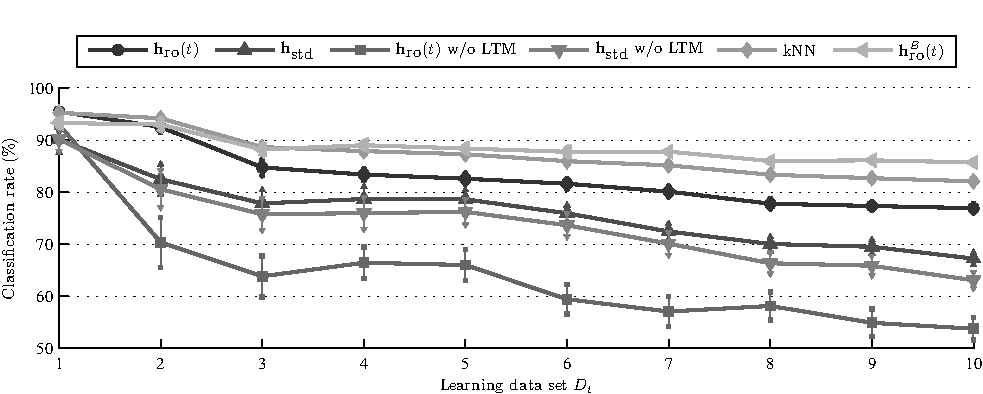
\includegraphics[width=0.98\linewidth]{c1_fig5_1} \label{fig:c1_AddExtErr} }
  \\
  \subfloat[Compression]{
 	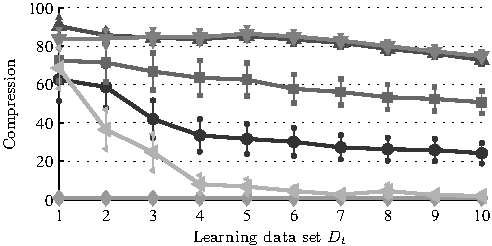
\includegraphics[width=0.46\linewidth]{c1_fig5_2} \label{fig:c1_AddExtCpn} }
   \subfloat[Convergence time]{
 	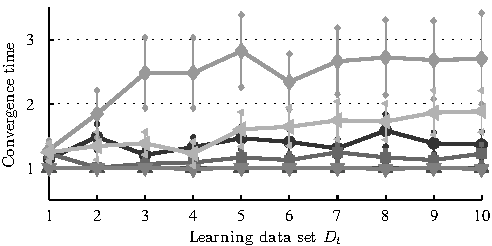
\includegraphics[width=0.46\linewidth]{c1_fig5_3} \label{fig:c1_AddExtEpo} }
	\end{minipage} }
  \caption{Average classification rate, compression, and convergence time of the ACS versus learning block during the enrollment scenario. Performance was evaluated with and without LTM for $\textbf{h}_\text{ro}(t)$ and $\textbf{h}_\text{std}$. Error bars correspond to the 90\% confidence interval. The performance for fuzzy ARTMAP with $\textbf{h}_\text{ro}^B(t)$ and \textit{k}NN during batch learning are shown for reference}
	\label{fig:c1_AddExt}
\end{figure}
%------------------------------------------------------------------------------%

As the amount of training data and the complexity of the decision boundaries increase, all hyperparameters settings follow the same degradation in classification rate. After learning all data, the highest performance is obtained with batch learning (85.6$\pm$0.3\% for $\textbf{h}_\text{ro}^B(t)$ and 82.3$\pm$0.1\% for \textit{k}NN), followed by incremental learning with $\textbf{h}_\text{ro}(t)$ and the LTM (77$\pm$1\%), $\textbf{h}_\text{std}$ with and without the LTM (67$\pm$1\% and 63$\pm$2\%), and finally $\textbf{h}_\text{ro}(t)$ without the LTM (54$\pm$2\%).

However, higher classification rate comes with a cost. Figure \ref{fig:c1_AddExtCpn} shows that compression, when using $\textbf{h}_\text{ro}(t)$ with the LTM starts lower than that obtained without LTM (63$\pm$11 versus 69$\pm$11), decreases to 32$\pm$8 at $D_5$ (compared to 63$\pm$9 without the LTM), and does not change significantly afterwards. Moreover, the average number of training epochs needed when using LTM (1.4$\pm$0.1) is higher than that of $\textbf{h}_\text{ro}(t)$ without LTM (1.1$\pm$0.1), confirming that using a LTM with larger data sets for validation leads to a greater number of training epochs (Figure \ref{fig:c1_AddExtEpo}).

Figure \ref{fig:c1_AddExt} also underline the necessity of storing validation data from all classes when fuzzy ARTMAP is trained with $\textbf{h}_\text{std}$. The networks selected when using LTM are more accurate, yet only more complex on $D_1$, compared to networks selected without the LTM. After incremental learning of 10 blocks with $\textbf{h}_\text{std}$ and LTM, classification rate is 5$\pm$4\% higher and compression is comparable to that obtained with $\textbf{h}_\text{std}$ without LTM. In both cases, convergence time with $\textbf{h}_\text{std}$ is one.
For fuzzy ARTMAP trained with $\textbf{h}_\text{ro}(t)$ and without LTM, Table \ref{tab:c1_AddEvo} shows that since $D_t^\text{f}$, where $2\leq t\leq10$, is only composed of one class ($C_{k'}(t)$), optimization is performed according to that class at the expense of all others ($\{C_k(t)\in \Omega|k\neq k'\}$).
While the classification rate for the class learned at a time $t$, $C_{k'}(t)$, is typically high (above 80\%, except for classes $C_2$ and $C_5$), the average overall classification rate for $\{C_k(t)\in \Omega|k\neq k'\}$ degrades considerably (ends at about $54\%$ after $D_{10}$).
In contrast, by estimating the fitness with LTM, PSO optimization is performed according to all classes and, although classification rate for $C_{k'}(t)$ is lower than without the LTM for all learning blocks, it is always significantly higher for $\{C_k^t\in \Omega|k\neq k'\}$.

%-------------- Classification rate per class for learned class ---------------%
\begin{table}[t]
  \small
  \centering
  \caption{Average classification rate achieved by the ACS for the added classes with each learning block $D_t$ for one class presentation order during the enrollment scenario. The classification rate of the new class added with $D_t$ ($C_{k'}(t)$) is presented with that of the remaining classes present at that time ($\{C_k^t\in \Omega|k\neq k'\}$). Each cell is presented in percentage and with the 90\% confidence interval}
  \begin{tabular}{|l|l|lllllllll|}
  	\hline
		%-- Header
		Training & $D_t$ & $D_{2}$ & $D_{3}$ & $D_{4}$ & $D_{5}$ & $D_{6}$ & $D_{7}$ & $D_{8}$ & $D_{9}$ & $D_{10}$\\\cline{2-11}
		strategy & $C_{k'}(t)$ &  11 &  5 &  4 &  8 &  9 &  7 &  3 &  6 &  2
		\\ \hline \hline

		%-- Hrop w/ LTM
		 & Class. rate for & 90 & 84 & 95 & 99 & 71 & 75 & 68 & 89 & 49	\\ 
		$\textbf{h}_\textnormal{ro}(t)$ & $C_{k'}(t)$ & $\pm 6$ &$\pm 5$ &$\pm 4$ &$\pm 1$ &$\pm 8$ &$\pm 5$ & $\pm 7$ & $\pm 4$ & $\pm 5$	\\ \cline{2-11} 
		w/ LTM &  Class. rate for & 94 & 76 & 79 & 80 & 82 & 79 & 78 & 76 & 77 \\ 
		& $\{C_{k'}(t)\in\Omega|k\neq k'\}$ & $\pm 1$ & $\pm 4$ & $\pm 3$ & $\pm 2$
		& $\pm 2$ & $\pm 2$ & $\pm 2$ & $\pm 2$ & $\pm 2$
		\\ \hline
		
		%-- Hrop w/o LTM
		 & Class. rate for & 100 & 95 & 96 & 98 & 87 & 88 & 77 & 91 & 72 \\ 
		$\textbf{h}_\textnormal{ro}(t)$ & $C_{k'}(t)$ & $\pm 1$ & $\pm 2$ & $\pm 2$ & $\pm 1$ & $\pm 4$ & $\pm 4$ & $\pm 13$ & $\pm 7$ & $\pm 11$	\\ \cline{2-11} 
		w/o LTM & Class. rate for & 31 & 36 & 54 & 61 & 48 & 51 & 56 & 47 & 52 \\ 
		& $\{C_{k'}(t)\in\Omega|k\neq k'\}$ &$\pm 22$ &$\pm 16$ &$\pm 10$ &$\pm 8$
		& $\pm 6$ & $\pm 9$ & $\pm 9$ & $\pm 6$ & $\pm 6$
		\\ \hline
	\end{tabular}
	\label{tab:c1_AddEvo}
\end{table}
%------------- /Classification rate per class for learned class ---------------%

%------------------------ Classification rate per class -----------------------%
\begin{table*}[tb]
  \small
  \centering
  \caption{Average classification rate per class for one class order presentation of the enrollment incremental learning scenario for $\textbf{h}_\text{ro}(t)$ and $\textbf{h}_\text{std}$, with and without the LTM. Results are obtained after enrollment of all classes $C_k\in\Omega$. Each cell is presents the classification rate in percentage along with the 90\% confidence interval}
  \footnotesize{
  \begin{tabular}{|l|lllllllllll|l|}
  	\hline
    Training &\multicolumn{11}{l|}{$C_k \in \Omega$} &\multirow{2}{*}{$\Omega$}
    \\ \cline{2-12}
    strategy &{\bf 1} &{\bf 2} &{\bf 3}  &{\bf 4}  &{\bf 5} & 
    {\bf 6} &{\bf 7} &{\bf 8} &{\bf 9} &{\bf 10} &{\bf 11} &
    \\ \hline \hline
		\multirow{2}{*}{$\textbf{h}_\text{ro}(t)$ w/ LTM}
		& 85 & 49 & 91 & 73 & 49 & 88 & 81 & 70 & 82 & 61 & 91 & 77
		\\ 
 		& $\pm 5$ & $\pm 5$ & $\pm 5$ & $\pm 4$ & $\pm 9$ & $\pm 5$ & $\pm 4$
 		& $\pm 7$ & $\pm 4$ & $\pm 7$ & $\pm 3$ & $\pm 1$
 		\\ \hline 
		\multirow{2}{*}{$\textbf{h}_\text{std}$ w/ LTM}
		& 62 & 5 & 84 & 56 & 93 & 78 & 67 & 32 & 83 & 37 & 77 & 67
		\\ 
		& $\pm 24$ & $\pm 4$ & $\pm 5$ & $\pm 6$ & $\pm 6$ & $\pm 4$ & $\pm 5$
		& $\pm 7$ & $\pm 2$ & $\pm 7$ & $\pm 4$ & $\pm 1$
		\\ \hline \hline 
		\multirow{2}{*}{$\textbf{h}_\text{ro}(t)$ w/o LTM}
		& 62 & 72 & 45 & 66 & 21 & 73 & 61 & 37 & 67 & 47 & 39 & 54
		\\ 
		& $\pm 24$ & $\pm 11$ & $\pm 25$ & $\pm 19$ & $\pm 19$ & $\pm 21$ 
		& $\pm 17$ & $\pm 25$ & $\pm 12$ & $\pm 17$ & $\pm 25$ & $\pm 2$
		\\ \hline 
		\multirow{2}{*}{$\textbf{h}_\text{std}$ w/o LTM}
		& 36 & 7 & 81 & 47 & 87 & 78 & 68 & 43 & 81 & 40 & 75 & 63
		\\ 
		& $\pm 8$ & $\pm 5$ & $\pm 8$ & $\pm 10$ & $\pm 7$ & $\pm 5$ & $\pm 7$
		& $\pm 11$ & $\pm 4$ & $\pm 7$ & $\pm 6$ & $\pm 2$
		\\ \hline 
	\end{tabular} }
	\label{tab:c1_AddExt}
\end{table*}
%------------------------ Classification rate per class -----------------------%

As mentioned, when the decision boundaries between class distributions are complex, it is difficult for the ACS to maintain a high classification rate with compact fuzzy ARTMAP networks. As classes are added to the ACS using $\textbf{h}_\text{std}$, the recognition categories created for new classes tend to expand into the boundaries of the older class distributions. The order in which classes are learned may then prove crucial for optimal performance. With the class presentation order given in Table \ref{tab:c1_AddEvo} and Table \ref{tab:c1_AddExt}, excepted for class $C_2$, which contains only 39 learning patterns, classification rates obtained for the latest classes added to the system using $\textbf{h}_\text{ro}(t)$ with LTM (classes $C_3$, $C_6$, $C_7$, and $C_9$) is significantly higher than those obtained using without LTM. The performance of these later classes are obtained at the expense of those present in previous blocks. However, no matter the choice of hyperparameters, classes $C_1$ and $C_3$ are not greatly affected by the addition of latter classes, suggesting that data distributions of classes $C_1$ and $C_3$ do not overlap those of classes $C_3$, $C_6$, $C_7$, and $C_9$.

%------------------------------------------------------------------------------%
%------------------------------------------------------------------------------%
\subsubsection{Update scenario}

%------------------------------------------------------------------------------%
\begin{figure*}[!t]
  \centering
	\fbox{\begin{minipage}{0.97\linewidth}\centering
  \subfloat[Classification rate]{
  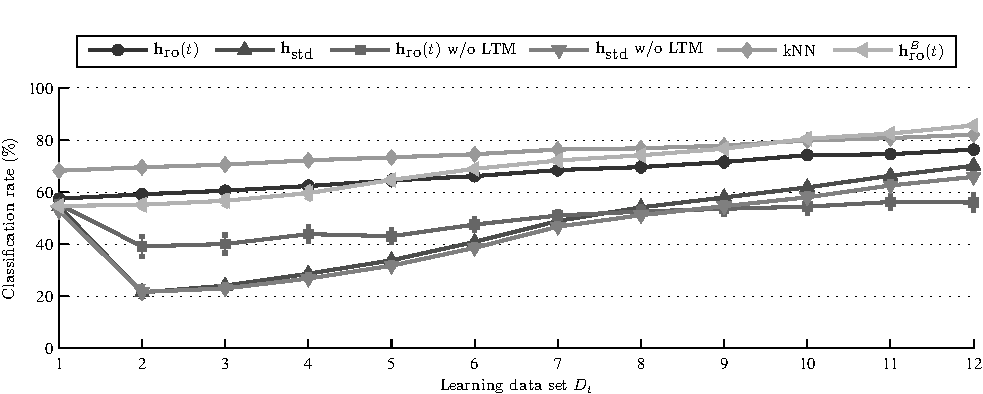
\includegraphics[width=0.98\linewidth]{c1_fig6_1} \label{fig:c1_RefExtErr} }
	\\
	\subfloat[Compression]{
  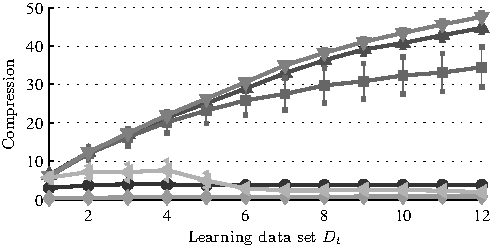
\includegraphics[width=0.48\linewidth]{c1_fig6_2} \label{fig:c1_RefExtCpn} }
  \subfloat[Convergence time]{
  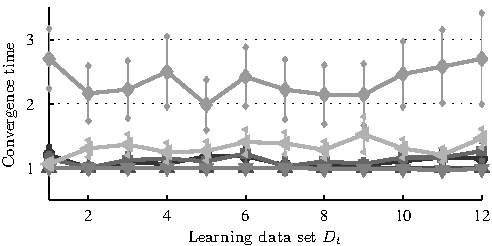
\includegraphics[width=0.48\linewidth]{c1_fig6_3} \label{fig:c1_RefExtEpo} }
	\end{minipage} }
 	\caption{Average classification rate, compression, and convergence time of the ACS versus learning block during the update scenario. Performance was evaluated with and without LTM for $\textbf{h}_\text{ro}(t)$ and $\textbf{h}_\text{std}$. Error bars correspond to the 90\% confidence interval. The performance for fuzzy ARTMAP with $\textbf{h}_\text{ro}^B(t)$ and \textit{k}NN during batch learning are shown for reference}
	\label{fig:c1_RefExt}
\end{figure*}
%------------------------------------------------------------------------------%

In the update scenario, all classes are defined from the start in $D_1$ with only 10\% of the available learning data. While \textit{k}NN yields a classification rate of 68.1$\pm$0.4 after learning $D_1$, the classification rate of the ACS for all system parameters settings starts below 60\%. This indicates that decision boundaries are very complex, and learning $D_1$ with limited data from each class is a difficult task for the ACS. As it was presented in \cite{granger08, connolly08}, this shows the importance of $D_1$ when fuzzy ARTMAP undergoes incremental learning, as it forms the basis for future updates with video data. An ACS should then be initiated with enough representative data from the environment.

At the beginning of the update process ($t \leq 4$), using more validation data with the LTM results in an increase in classification rates of the ACS when $\textbf{h}_\text{ro}(t)$ is used during incremental learning. Moreover, the ACS with $\textbf{h}_\text{ro}(t)$ and LTM gives a similar classification rate as the reference systems, minus the effects of knowledge corruption. While the classification rate with $\textbf{h}_\text{ro}(t)$ starts at 57.4$\pm$0.5\% at $t=1$ and steadily increases up to 76$\pm$1\% at $t=10$, classification rate with View the MathML source starts at 55$\pm$1\%, reaches 60$\pm$2\% at $t=4$, and increases faster than that of $\textbf{h}_\text{ro}(t)$ to end at 85.6$\pm$0.3\%. This sudden increase in performance also correspond to a decrease in compression. While compression of $\textbf{h}_\text{ro}(t)$ starts at 3$\pm$1 at $t=1$ and remains steady at 4$\pm$1 for $ 2\leq t \leq12$, compression of $\textbf{h}_\text{ro}^B(t)$ increases from 6$\pm$1 ($t=1$) to 8$\pm$2 ($t=4$), and suddenly drops to 2.4$\pm$0.4 ($t=7$) without changing significantly afterwards. Overall, $\textbf{h}_\text{ro}^B(t)$ needed about 1.7 more nodes than $\textbf{h}_\text{ro}(t)$ to obtained a classification rate 10\% higher. It outperforms \textit{k}NN classification rate, compression, and convergence time.

Meanwhile, classification rates obtained with $\textbf{h}_\text{std}$ and $\textbf{h}_\text{ro}(t)$ (without LTM) decrease considerably $t=2$ (22$\pm$2\% for both cases of $\textbf{h}_\text{std}$ and to 39$\pm$4\% for $\textbf{h}_\text{ro}(t)$ without LTM). However, updating all classes using $\textbf{h}_\text{std}$ increases overall performances (classification rate increases by about 15\% with LTM, 13\% without LTM, and with a higher compression in both cases), while using $\textbf{h}_\text{ro}(t)$ without LTM only results in a gain in compression (classification rates after learning $D_1$ and $D_{12}$ that are both 59$\pm$2\%).

As with the enrollment learning scenario, Table \ref{tab:c1_RefEvo} shows that the ACS without the LTM is only optimized for classes updated with each $D_t$. Classification rates for $C_{k'}(t)$ are either higher than or comparable to those of $\textbf{h}_\text{ro}(t)$ with the LTM, while the classification rates for $\{C_k(t)\in \Omega|k\neq k'\}$ are degraded compared to those obtained when using the LTM. Coarse decision boundaries created at the beginning of the update process ($D_2$) are refined when new data becomes available. As the overall classification rate increases, the difference between $C_{k'}(t)$ and $\{C_k(t)\in \Omega|k\neq k'\}$ decreases (from 45$\pm$5\% at $t=2$, to 19$\pm$7\% at $t=12$).

Unlike with the enrollment scenario, Table \ref{tab:c1_RefEvo} and Table \ref{tab:c1_RefExt} show that individual classification rates obtained after learning all data are less sensitive to class order presentation when all classes defined in $D_1$. Classification rates of $C_{k'}(t)$ obtained with $\textbf{h}_\text{ro}(t)$ and LTM in Table \ref{tab:c1_RefEvo} are no longer systematically below those of $\textbf{h}_\text{ro}(t)$ without LTM. Moreover, individual classification rates from Table \ref{tab:c1_RefExt} differ less from the overall classification rate and their dispersion is lower. As an example, $\textbf{h}_\text{ro}(t)$ with LTM yield a standard deviation of 16 for the individual classification rates during the enrollment scenario, and a standard deviation of 14 for the update scenario. This lead to higher global classification rates over all classes.

%-------------- Classification rate per class for learned class ---------------%
\begin{center}
\begin{table*}[tb]
  \small
  \centering
  \caption{Average classification rate achieved by the ACS for the updated classes with each learning block $D_t$ for one class presentation order during the update scenario. The classification rate of the updated class with $D_t$ ($C_{k'}(t)$) is presented with that of the remaining classes ($\{C_k^t\in \Omega|k\neq k'\}$). Each cell is presented in percentage and with the 90\% confidence interval}
  \footnotesize{
  \begin{tabular}{|l|l|lllllllllll|}
  \hline
	%-- Header
	Training & $D_t$ & $D_{2}$ & $D_{3}$ & $D_{4}$ & $D_{5}$ & $D_{6}$ & $D_{7}$ & $D_{8}$ & $D_{9}$ & $D_{10}$ & $D_{11}$ & $D_{12}$	\\ \cline{2-13}
	strategy & $C_{k'}(t)$ & 11 & 5 & 1 & 7 & 9 & 3 & 10 & 4 & 8 & 6 & 2
	\\ \hline \hline

	%-- Hrop w/ LTM
	 & Class. rate for & 90 & 77 & 98 & 88 & 87 & 98 & 78 & 87 & 70 & 92 & 92
	\\ 
	$\textbf{h}_\textnormal{ro}(t)$ & $C_{k'}(t)$ & $\pm$4 & $\pm$6 & $\pm$2 & $\pm$3 & $\pm$5 & $\pm$1	& $\pm$7 & $\pm$6 & $\pm$12 & $\pm$4 & $\pm$4
	\\ \cline{2-13} 
	w/ LTM & Class. rate for & 55 & 62 & 60 & 64 & 68 & 65 & 70 & 74 & 76 & 74 & 73
	\\ 
	 & $\{C_{k'}(t)\in\Omega|k\neq k'\}$ & $\pm$1 & $\pm$1 & $\pm$1 & $\pm$2
	& $\pm$2 & $\pm$3 & $\pm$2 & $\pm$3 & $\pm$3 & $\pm$3 & $\pm$3
	\\ \hline \hline
	%-- Hrop w/0 LTM
	 & Class. rate for & 98 & 86 & 95 & 82 & 91 & 99 & 80 & 85 & 72 & 90 & 74 \\ 
	 $\textbf{h}_\textnormal{ro}(t)$ & $C_{k'}(t)$ & $\pm$2 & $\pm$7 & $\pm$3 & $\pm$8 & $\pm$2 & $\pm$1 & $\pm$7 & $\pm$7 & $\pm$13 & $\pm$5 & $\pm$13	\\ \cline{2-13} 
	w/o LTM & Class. rate for & 37 & 32 & 36 & 39 & 43 & 46 & 50 & 51 & 51 & 59 & 51 \\ 
	& $\{C_{k'}(t)\in\Omega|k\neq k'\}$ & $\pm$8 & $\pm$10 & $\pm$6 & $\pm$6
	& $\pm$6 & $\pm$4 & $\pm$5 & $\pm$7 & $\pm$8 & $\pm$7 & $\pm$10
	\\ \hline

	\end{tabular} }
	\label{tab:c1_RefEvo}
\end{table*}
\end{center}
%-------------- Classification rate per class for learned class ---------------%

%------------------------ Classification rate per class -----------------------%
\begin{table*}[tb]
  \small
  \centering
  \caption{Average classification rate per class for one class order presentation of the update incremental learning scenario for $\textbf{h}_\text{ro}(t)$ and $\textbf{h}_\text{std}$, with and without the LTM. Results are obtained after update of all classes $C_k\in\Omega$. Each cell is presents the classification rate in percentage along with the 90\% confidence interval}
  \footnotesize{
  \begin{tabular}{|l|lllllllllll|l|} \hline
    Training &\multicolumn{11}{l|}{$C_k \in \Omega$} &\multirow{2}{*}{$\Omega$}
    \\ \cline{2-12}
    strategy &{\bf 1} &{\bf 2} &{\bf 3}  &{\bf 4}  &{\bf 5} & 
    {\bf 6} &{\bf 7} &{\bf 8} &{\bf 9} &{\bf 10} &{\bf 11} &
    \\ \hline \hline
		\multirow{2}{*}{$\textbf{h}_\text{ro}(t)$ w/ LTM}
		& 83 & 92 & 92 & 82 & 53 & 92 & 82 & 69 & 70 & 59 & 60 & 76
		\\ 
		& $\pm 8$ & $\pm 5$ & $\pm 5$ & $\pm 8$ & $\pm 8$ & $\pm 4$ & $\pm 2$
		& $\pm 12$ & $\pm 14$ & $\pm 7$ & $\pm 11$ & $\pm 1$
		\\ \hline 
		\multirow{2}{*}{$\textbf{h}_\text{std}$ w/ LTM} 
		& 57 & 11 & 94 & 38 & 83 & 85 & 78 & 34 & 84 & 52 & 78 & 70
		\\ 
		& $\pm 28$ & $\pm 5$ & $\pm 3$ & $\pm 9$ & $\pm 5$ & $\pm 5$ & $\pm 6$
		& $\pm 6$ & $\pm 2$ & $\pm 5$ & $\pm 4$ & $\pm 1$
		\\ \hline \hline
		\multirow{2}{*}{$\textbf{h}_\text{ro}(t)$ w/o LTM}
		& 57 & 74 & 54 & 59 & 18 & 56 & 52 & 69 & 72 & 41 & 44 & 56
		\\ 
		& $\pm 28$ & $\pm 14$ & $\pm 27$ & $\pm 25$ & $\pm 15$ & $\pm 25$ 
		& $\pm 20$ & $\pm 18$ & $\pm 12$ & $\pm 19$ & $\pm 25$ & $\pm 3$
		\\ \hline 
		\multirow{2}{*}{$\textbf{h}_\text{std}$ w/o LTM} 
		& 38 & 3 & 84 & 38 & 89 & 83 & 70 & 44 & 81 & 38 & 71 & 66
		\\ 
		& $\pm 8$ & $\pm 3$ & $\pm 6$ & $\pm 9$ & $\pm 8$ & $\pm 5$ & $\pm 7$
		& $\pm 7$ & $\pm 3$ & $\pm 7$ & $\pm 6$ & $\pm 2$
		\\ \hline 
	
	\end{tabular} }
	\label{tab:c1_RefExt}
\end{table*}
%------------------------ Classification rate per class -----------------------%

%------------------------------------------------------------------------------%
%------------------------------------------------------------------------------%
\subsection{Experiment ($B$) -- Impact of dynamic optimization}

Figure \ref{fig:c1_AddDyn} and Figure \ref{fig:c1_RefDyn} present the average classification rate, compression, and convergence time achieved by the ACS with a LTM and with system parameters that are optimized using: dynamic optimization with DNPSO ($\textbf{h}_\text{dnc}(t)$), DNPSO on only $D_1$ and are then fixed ($\textbf{h}_\text{dnc}(1)$), static optimization with DNPSO ($\textbf{h}_\text{stc}(t)$), static optimization with canonical PSO ($\textbf{h}_\text{cnl}(t)$), and the reference batch learning method ($\textbf{h}_\text{ro}^B(t)$). The evolution of hyperparameters found via $\textbf{h}_\text{dnc}(t)$ is shown for all class presentation order in Figure \ref{fig:c1_AddDynHp} and Figure \ref{fig:c1_RefDynHp} after incremental learning of different blocks for both incremental learning scenario. Figure \ref{fig:c1_AddDynSwarm} and Figure \ref{fig:c1_RefDynSwarm} shows the position of the swarms at different moments in time for the same class presentation order used in Table \ref{tab:c1_AddEvo}, Table \ref{tab:c1_AddExt}, Table \ref{tab:c1_RefEvo} and Table \ref{tab:c1_RefExt}.

%------------------------------------------------------------------------------%
\subsubsection{Enrollment scenario}

%--------------------------- Perfomances - Addition ---------------------------%
\begin{figure}[!b]
  \centering
	\fbox{\begin{minipage}{0.97\linewidth}\centering
  \subfloat[Classification rate]{
 	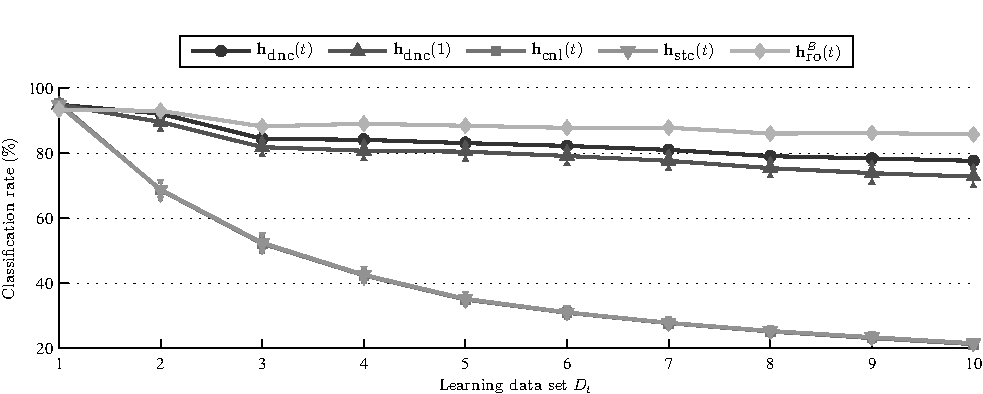
\includegraphics[width=0.98\linewidth]{c1_fig7_1} \label{fig:c1_AddDynErr} }
  \\
  \subfloat[Compression]{
 	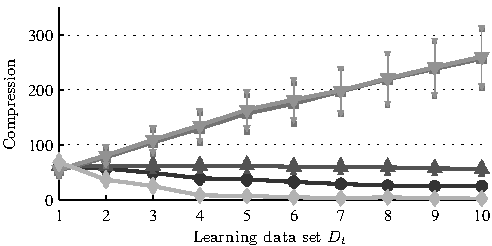
\includegraphics[width=0.48\linewidth]{c1_fig7_2} \label{fig:c1_AddDynCpn} }
  \subfloat[Convergence time]{
 	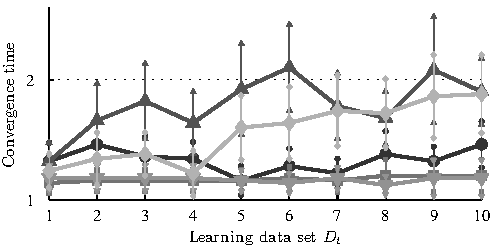
\includegraphics[width=0.48\linewidth]{c1_fig7_3} \label{fig:c1_AddDynEpo} }
	\end{minipage} }
  \caption{Average classification rate, compression, and convergence time of the ACS versus learning block during the enrollment scenario. Performance was evaluated with the LTM for $\textbf{h}_\text{dnc}(t)$, $\textbf{h}_\text{dnc}(1)$, $\textbf{h}_\text{stc}(t)$, and $\textbf{h}_\text{cnl}(t)$. Error bars correspond to the 90\% confidence interval. The performance for fuzzy ARTMAP with $\textbf{h}_\text{ro}^B(t)$ during batch learning is shown for reference}
	\label{fig:c1_AddDyn}
\end{figure}
%--------------------------- Perfomances - Addition ---------------------------%

Figure \ref{fig:c1_AddDyn} illustrates that, when the proposed ACS is used with a static optimization algorithm ($\textbf{h}_\text{stc}(t)$ and $\textbf{h}_\text{cnl}(t)$), classification rate declines significantly during the enrollment learning scenario. Unlike with dynamic optimization ($\textbf{h}_\text{dnc}(t)$), static optimization algorithms does not automatically update the fitness corresponding to the position of each particle's personal best when a new $D_t$ becomes available, requiring the $\textit{FAM}_n$ networks to be trained on $D_t^\text{t}$ (Line \ref{l:c1_trnUpdate}). As classes are added to the ACS, decision boundaries become more complex and fitness values estimated on $D_t^\text{f}$, initially 100\% after learning $D_1$, decline in time. The particle's personal best positions of static PSO algorithms ($\textbf{h}_\text{stc}(t)$ and $\textbf{h}_\text{cnl}(t)$) are thus never redefined, and the $\textit{FAM}_n$ networks, which learn two classes on $D_1$, are never updated afterwards. The rest of the learning process is then always based on a $\textit{FAM}_n$ neural network that learned only two classes.

When using a dynamic PSO algorithm, Figure \ref{fig:c1_AddDynHp} shows that $\textbf{h}_\text{dnc}(t)$ changes such that fuzzy ARTMAP can maintain a higher classification rate with low confidence interval. Although the confidence interval for all hyperparameters tends to be large, Figure \ref{fig:c1_AddDynHp} still indicates that they vary according to some pattern no matter class presentation order. Moreover, the impact of new data on fuzzy ARTMAP hyperparameters does not appear to diminished as more classes are presented to ACS with $\textbf{h}_\text{dnc}(t)$.

%-------------------------- HP evolution - Addition ---------------------------%
\begin{figure}[t]
  \centering
	\fbox{
 	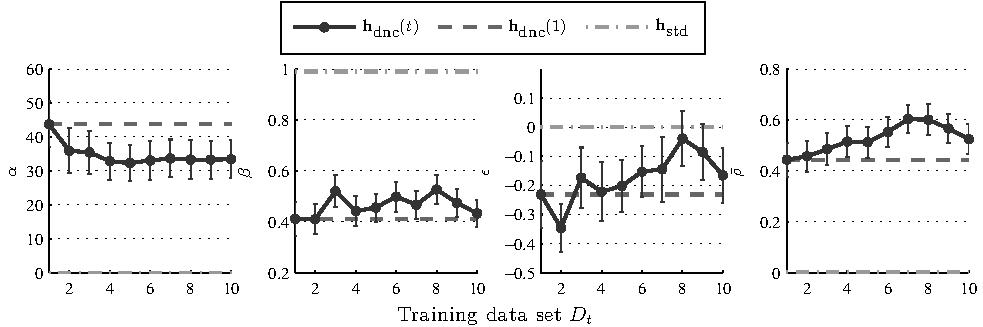
\includegraphics[width=0.97\linewidth]{c1_fig8}
 	}
  \caption{ Evolution of hyperparameter values obtained with the ACS using $\textbf{h}_\text{dnc}(t)$ compared to the ACS based on $\textbf{h}_\text{dnc}(t)$ and $\textbf{h}_\text{std}$(t) during the enrollment scenario. The mean of each hyperparameter is shown with its 90\% confidence interval}
	\label{fig:c1_AddDynHp}
\end{figure}
%-------------------------- HP evolution - Addition ---------------------------%

While $\alpha$ changes significantly only once from 44$\pm$7 at $t=1$ to 36$\pm$7 at $t=2$, $\beta$ starts at 0.40$\pm$0.07 and changes significantly four times at $t\in\{3,4,8,9\}$ (to 0.52$\pm$0.06, 0.44$\pm$0.06, 0.53$\pm$0.06, and 0.43$\pm$0.06). Hyperparameter $\epsilon$ starts at $-0.23\pm$0.11 and changes four times at $t\in\{2,3,8,10\}$ (to $-0.35\pm$0.08, $-0.17\pm$0.10, $-0.04\pm$0.09, and $-0.17\pm$0.09). Finally, $\bar{\rho}$  starts at 0.44$\pm$0.07, increases to 0.60$\pm$0.05 at $t=7$ and decreases to 0.52$\pm$0.06. Figure \ref{fig:c1_AddDynSwarm} shows the evolution of particles in the DNPSO swarm mapped in two dimensions space using Sammon's mapping (\cite{kim09}). As expected, the classification rates estimated for most of the networks after $D_1$ are 100\%. As classes are added to the system, DNPSO subswarms moves in the hyperparameters space as new peaks appear and disappear in the objective function. Even if the global best solution obtained during incremental learning is not always near the global best obtained with $\textbf{h}_\text{ro}^B(t)$, the latter is always found by one of the DNPSO subswarms. This indicates that the optimization space defined by fuzzy ARTMAP hyperparameters adjustment for the enrollment scenario does in fact correspond to a type III optimization environment (see Section \ref{sec:c1_adaptation}).

%--------------------------- HP evolution - Addition --------------------------%
\begin{figure}[t]
  \centering
	\fbox{ 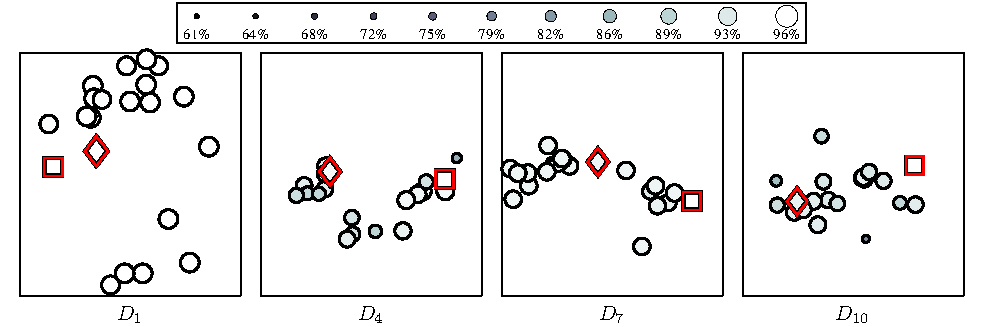
\includegraphics[width=0.97\linewidth]{c1_fig9} }
	\caption{A two-dimensional Sammon's mapping illustrating the evolution of each particle's personal best, and the swarm's global best positions when the proposed ACS performs incremental learning with $\textbf{h}_\text{dnc}(t)$ (diamond) for the enrollment scenario. The global best particle position obtained for batch learning with $\textbf{h}_\text{ro}^B(t)$ (square) is also shown for reference. Positions are shown along the estimation of $f(\textbf{h},t)$ (see legend) when the optimization stopping conditions have been reached for different points in time ($t\in\{1,4,7,10\}$) during the update scenario for one replication and the same class presentation order presented in the previous sections}
	\label{fig:c1_AddDynSwarm}
\end{figure}
%-------------------------- HP evolution - Addition ---------------------------%

Beside the reference $\textbf{h}_\text{ro}^B(t)$, the ACS based on $\textbf{h}_\text{dnc}(t)$ achieves the highest (78$\pm$1\%), followed by $\textbf{h}_\text{dnc}(1)$ (72$\pm$3\%), $\textbf{h}_\text{stc}(t)$, and $\textbf{h}_\text{cnl}(t)$ (both at 21$\pm$1\%). Compared to $\textbf{h}_\text{dnc}(1)$, classification rates with $\textbf{h}_\text{dnc}(t)$ starts 94.8$\pm$0.6\% and become significantly different to that of $\textbf{h}_\text{dnc}(1)$ as of $t=2$. As in previous results, a lower compression (25$\pm$1 at $t=10$) is necessary to maintain higher classification rates.

Results with the MoBo data base confirms the results obtained with the IIT-NRC data base. However, since the acquisition of the MoBo data is more constrained than that of the IIT-NRC data, class distributions $p_k(\textbf{a})$ are more compact and are less likely to vary significantly from one block to the next. As Table \ref{tab:c1_AddMobo} shows, classification rates are comparable for $\textbf{h}_\text{dnc}(t)$ and $\textbf{h}_\text{dnc}(1)$, and compressions are twice as high as those obtained with the IIT-NRC data base.

%------------------------------- Results - MoBo -------------------------------%
\begin{table*}[tb]
  \small
  \centering
  \caption{Average classification rate (in percentage) and compression after incremental learning of all the MoBo data base for the enrollment scenario. Each cell is presented with the 90\% confidence interval}
  \begin{tabular*}{\linewidth}{@{\extracolsep{\fill}}|l|llll|}
  	\hline
    Performance indicator      & $\textbf{h}_\text{dnc}(t)$
															 & $\textbf{h}_\text{dnc}(1)$
															 & $\textbf{h}_\text{stc}(t)$
															 & $\textbf{h}_\text{cnl}(t)$
    \\ \hline 
    Classification rate & $79\pm2\%$ & $78\pm4\%$ & $20\pm1\%$ & $20\pm1\%$
    \\ 
    Compression         & $45\pm3$ & $97\pm80$ & $480\pm10$ & $480\pm10$
    \\ \hline
	\end{tabular*}
	\label{tab:c1_AddMobo}
\end{table*}
%------------------------------- Results - MoBo -------------------------------%

%------------------------------------------------------------------------------%
%------------------------------------------------------------------------------%
\subsubsection{Update scenario}

%------------------------------------------------------------------------------%
\begin{figure}[!t]
  \centering
	\fbox{\begin{minipage}{0.97\linewidth}\centering
   \subfloat[Classification rate]{
 		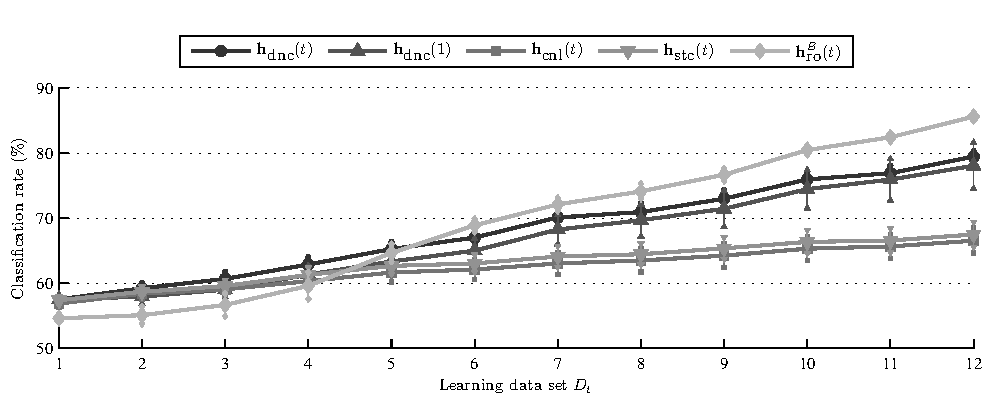
\includegraphics[width=0.98\linewidth]{c1_fig10_1} \label{fig:c1_RefDynErr} }
  \\
  \subfloat[Compression]{
 		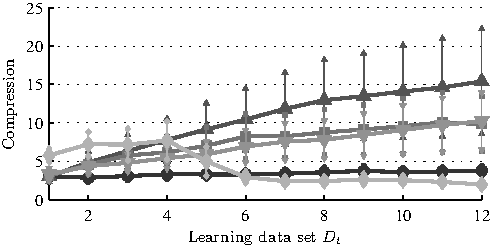
\includegraphics[width=0.48\linewidth]{c1_fig10_2} \label{fig:c1_RefDynCpn} }
  \subfloat[Convergence time]{
 		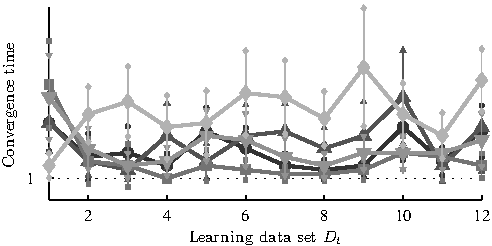
\includegraphics[width=0.48\linewidth]{c1_fig10_3} \label{fig:c1_RefDynEpo} }
	\end{minipage} }
	\caption{Average classification rate, compression, and convergence time of the ACS versus learning block during the update scenario. Performance was evaluated with the LTM for $\textbf{h}_\text{dnc}(t)$, $\textbf{h}_\text{dnc}(1)$, $\textbf{h}_\text{stc}(t)$, and $\textbf{h}_\text{cnl}(t)$. Error bars correspond to the 90\% confidence interval. The performance for fuzzy ARTMAP with $\textbf{h}_\text{ro}^B(t)$ during batch learning is shown for reference}
	\label{fig:c1_RefDyn}
\end{figure}
%------------------------------------------------------------------------------%


Figure \ref{fig:c1_RefDyn} also shows that using an ACS based on static optimization algorithms ($\textbf{h}_\text{stc}(t)$ and $\textbf{h}_\text{cnl}(t)$) results in poor incremental learning capabilities. In some cases, both DNPSO, applied without updating the personal best when new data is available ($\textbf{h}_\text{stc}(t)$), and canonical PSO ($\textbf{h}_\text{cnl}(t)$) algorithms find an hyperparameter vector that remains an optimum through during the entire learning process. But in other cases, the swarm stays in a region of the optimization space where classification rate does not improve and, as with the enrollment scenario, fitness corresponding to personal best positions does not improve and the $\textit{FAM}_n$ neural networks are never updated. Since the DNPSO algorithm, used without updating the personal best, is able to maintain diversity in the optimization space, it tends to provide a higher level of performance after learning all data but shows no significant differences with canonical PSO (68$\pm$2\% for $\textbf{h}_\text{stc}(t)$ versus 67$\pm$2\% $\textbf{h}_\text{cnl}(t)$). In both cases the average classification rate remains below 70\%.

As blocks of data are presented to the ACS during the update scenario, Figure \ref{fig:c1_RefDynHp} shows that all four hyperparameters are also adjusted during the update scenario. While, $\alpha$ steadily increases from 49$\pm$7 to 74$\pm$5, $\beta$ significantly changes five times ($t=\{2,5,9,10\}$) with values ranging from 0.26$\pm$0.06 to 0.48$\pm$0.07, $\epsilon$ changes two times ($t=\{2,7\}$) with values ranging from $-0.04\pm0.12$ to 0.11$\pm$0.12 and very high confidence intervals, and $\bar{\rho}$ changes five times ($t=\{2,5,9,10,11\}$) with values ranging from 0.62$\pm$0.08 to 0.82$\pm$0.06.

%--------------------------- HP evolution - Update ----------------------------%
\begin{figure}[ht]
  \centering
	\fbox{ 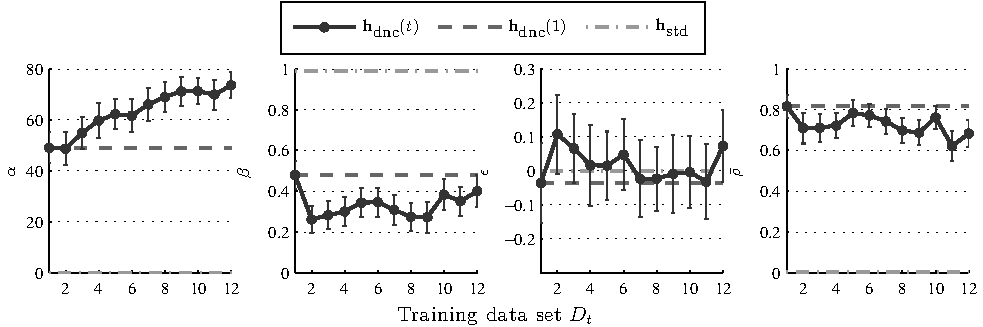
\includegraphics[width=0.97\linewidth]{c1_fig11} }
	\caption{Evolution of hyperparameter values obtained with the ACS using $\textbf{h}_\text{dnc}(t)$ compared to the ACS based on $\textbf{h}_\text{dnc}(t)$ and $\textbf{h}_\text{std}$(t) during the update scenario. The mean of each hyperparameter is shown with its 90\% confidence interval}
	\label{fig:c1_RefDynHp}
\end{figure}
%--------------------------- HP evolution - Update ----------------------------%

Like with the enrollment scenario, when observing the evolution of particles in the DNPSO swarm mapped in two dimensions space using Sammon's mapping, Figure \ref{fig:c1_RefDynSwarm} indicates the presence of a type III dynamic optimization environment (Section \ref{sec:c1_adaptation}). The personal best position of each particle are adjusted in response to peaks in the objective function $f(\textbf{h},t)$ that change position and values in time. However, since all classes are present in $D_1$, most of the feature space is define at the outset of the incremental learning process. Apart from the peak appearing in the middle of the optimization space at $t=4$, most of the changes in $f(\textbf{h},t)$ happen in the interval $4\leq t\leq8$.

%--------------------------- HP evolution - Update ----------------------------%
\begin{figure}[ht]
  \centering
 	\fbox{ 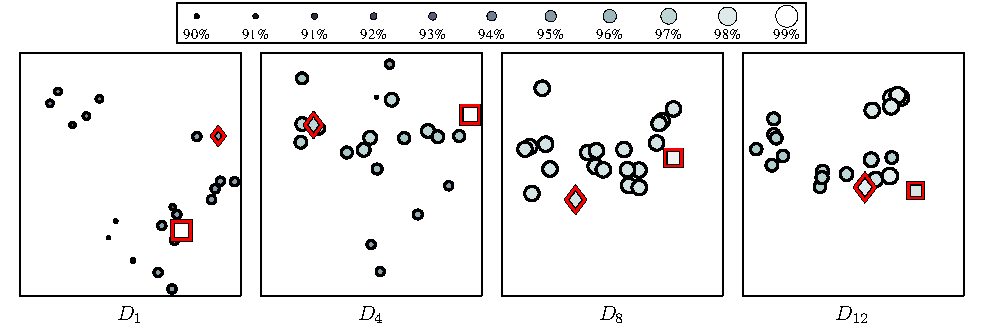
\includegraphics[width=0.97\linewidth]{c1_fig12}	}
	\caption{A two-dimensional Sammon's mapping illustrating the evolution of each particle's personal best, and the swarm's global best positions when the proposed ACS performs incremental learning with $\textbf{h}_\text{dnc}(t)$ (diamond) for the update scenario. The global best particle position obtained for batch learning with $\textbf{h}_\text{ro}^B(t)$ (square) is also shown for reference. Positions are shown along the estimation of $f(\textbf{h},t)$ (see legend) when the optimization stopping conditions have been reached for different points in time ($t\in\{1,4,8,12\}$) during the update scenario for one replication and the same class presentation order presented in the previous sections}
	\label{fig:c1_RefDynSwarm}
\end{figure}
%--------------------------- HP evolution - Update ----------------------------%

For the update scenario, the highest and more stable classification rate is achieved by dynamic optimization with $\textbf{h}_\text{dnc}(t)$ (Figure \ref{fig:c1_RefDyn}). Classification rates starts at 57.5$\pm$0.4\% and end at 79.4$\pm$0.9\%. It is almost always above classification rate obtained with $\textbf{h}_\text{dnc}(1)$ by at least 1\%. As shown in Figure \ref{fig:c1_RefDynCpn}, solutions obtained with $D_1$ are mostly heavy solutions that accommodate a complex input features space containing all classes. For $t>1$, those solutions yield large fuzzy ARTMAP neural networks, similar to those obtain in batch learning, and provide high classification rates. Moreover, the global best positions found at $t=1$ tend to remain in the vicinity of, at least, one subsequent local best position found during incremental learning, and of the global best positions found during batch learning (Figure \ref{fig:c1_RefDynSwarm}).

On the other hand, the ACS with $\textbf{h}_\text{dnc}(1)$ also find lighter solutions that performs also well on $D_1$, but then gives lower classification rate than the ACS with $\textbf{h}_\text{dnc}(t)$ when classes are updated. For $t\geq6$, when batch learning surpass incremental learning, those solutions do not perform as well as the larger ones, and the confidence interval for the classification rate grows from 1.4 at $t=4$ to 3.5 at $t=12$ while the latter for compression eventually grows to 7.

%------------------------------- Results - MoBo -------------------------------%
\begin{table*}[tb]
  \small
  \centering
  \caption{Average classification rate (in percentage) and compression after incremental learning of all the MoBo data base for the update scenario. Each cell is presented with the 90\% confidence interval}
  \begin{tabular*}{\linewidth}{@{\extracolsep{\fill}}|l|llll|}
  	\hline
    Performance indicator      & $\textbf{h}_\text{dnc}(t)$
															 & $\textbf{h}_\text{dnc}(1)$
															 & $\textbf{h}_\text{stc}(t)$
															 & $\textbf{h}_\text{cnl}(t)$
    \\ \hline
    Classification rate & $85\pm2\%$ & $88\pm3\%$ & $51\pm1\%$ & $52\pm1\%$
    \\
    Compression         & $11\pm2$ & $20\pm8$ & $36\pm9$ & $33\pm9$
    \\ \hline
	\end{tabular*}
	\label{tab:c1_RefMobo}
\end{table*}
%------------------------------- Results - MoBo -------------------------------%

Once again, results with the MoBo data base confirms the results obtained with the IIT-NRC data (Table \ref{tab:c1_RefMobo}). Classes in the MoBo data base are found to be more easily updated for $\textbf{h}_\text{dnc}(t)$ and $\textbf{h}_\text{dnc}(1)$. Both classification rates obtained with MoBo are over 5\% higher than those obtain on the IIT-NRC data. Since acquisition conditions are more constrained, $D_1$ data structure is now more representative of the entire learning data set and solutions found with $\textbf{h}_\text{dnc}(1)$ remain comparable to $\textbf{h}_\text{dnc}(t)$ in terms of classification rate. The average compression is also higher for all hyperparameters settings, but as with IIT-NRC, it is higher with $\textbf{h}_\text{dnc}(1)$. ACS using static optimization with MoBo also results in lighter solutions, those solutions yield lower classification rates.

%------------------------------------------------------------------------------%
%--------------------------------- Conclusion ---------------------------------%
\section{Conclusion}

In this chapter, an adaptive classification system (ACS) is proposed for video-based face recognition. It combines a fuzzy ARTMAP neural network classifier, dynamic particle swarm optimization (DPSO) algorithm, and a long term memory (LTM). This ACS uses a novel DPSO-based learning strategy to cojointly optimize the classifier weights, architecture, and user-defined hyperparameters such as classification rate is maximized during incremental learning of new data. This DPSO-based learning strategy reconsiders the four properties of a classification system capable of supervised incremental learning (as defined in \cite{polikar01}) in two ways. The $2^{nd}$ property is modified to include the storage and management of previously acquired learning data for unbiased validation and fitness estimation. To avoid knowledge corruption, and thereby maintain a high level of performance, a $5^{th}$ property is added to the others: a classifier must adapt its learning dynamics by adjusting its hyperparameters.

Using real-world video data bases, performance of this system is assessed in terms of classification rate and resource requirements, for different hyperparameter settings, with and without LTM. Overall results of experiments ($A$) and ($B$) demonstrate that optimizing fuzzy ARTMAP hyperparameters during incremental learning gives higher classification rates than when using standard or fixed hyperparameters ($\textbf{h}_\text{std}$ and $\textbf{h}_\text{dnc}(1)$). When property (5) of an incremental learning algorithm is applied, results indicate that, during incremental learning, fuzzy ARTMAP performance degrades unless some validation data are stored and updated in a LTM. Moreover, experiment ($B$) shows that, as more samples are learned by fuzzy ARTMAP with the LTM, peaks of the objective function (in the hyperparameters space) changes in time. Adjusting hyperparameters during incremental learning thus corresponds to a type III dynamic optimization problem and if a dynamic optimization algorithm is not employed to adjust classifier hyperparameters, then classification rate of fuzzy ARTMAP declines.

Results show that the proposed ACS requires more resources. Since the new DPSO-based learning strategy used by the ACS optimizes according to classification rate, it tends to produce fuzzy ARTMAP networks with a large number of $F_2$ layer nodes, and trains over longer convergence time. In order to keep the neural networks size and computational time to a minimum, future work would include designing an ACS that performs multi-objective optimization of fuzzy ARTMAP hyperparameters during supervised incremental learning. Moreover, results for both enrollment and update scenarios suggest that it may not be necessary to optimize fuzzy ARTMAP hyperparameters, weights, and architecture each time a new block of data becomes available. Since several training sequences are needed each time a fitness value is estimated, optimization is a costly process, and it would also be necessary to devise fitness-based detection measures that determines situations under which the ACS can benefit from incremental learning of blocks of data. Finally, devising a strategy to update the LTM with the most relevant data may improve performance and limit memory consumption.
\chapter{Evolution of heterogeneous ensembles through dynamic particle swarm optimization for video-based face recognition}

After performing mono-optimization of only one FAM network when new data is available, this chapter presents a second iteration of the supervised incremental learning strategy that optimizes a population of classifiers to create ensembles.
Whereas the previous study illustrates the impact of learning new data incrementally on the optimization environment, this chapter focuses on characterizing how genotype (\emph{i.e.}, hyperparameter) diversity affects classifier diversity and how this relationship can be used to evolve diversified ensembles of classifiers.
It was published in the Pattern Recognition journal (Elsevier) \cite{connolly11}. 

%----------------------------- Abstract & keywords ----------------------------%
%-- Paper objective
In this chapter, an incremental learning strategy based on dynamic particle swarm optimization (DPSO) is proposed to evolve heterogeneous ensembles of classifiers (where each classifier corresponds to a particle) in response to new reference samples.
This new strategy is applied to video-based face recognition, using an adaptive multiclassifier system (AMCS) that consists of a pool of fuzzy ARTMAP (FAM) neural networks for classification of facial regions, and a niching version of DPSO that optimizes all FAM parameters such that the classification rate is maximized.
%-- Results
Given that diversity within a dynamic particle swarm is correlated with diversity within a corresponding pool of base classifiers, DPSO properties are exploited to generate and evolve diversified pools of FAM classifiers, and to efficiently select ensembles among the pools based on accuracy and particle swarm diversity.
Performance of the proposed strategy is assessed in terms of classification rate and resource requirements under different incremental learning scenarios, where new reference data is extracted from real-world video streams.
%-- Results presentation - generality
Simulation results indicate the DPSO strategy provides an efficient way to evolve ensembles of FAM networks in an AMCS.
Maintaining particle diversity in the optimization space yields a level of accuracy that is comparable to AMCS using reference ensemble-based and batch learning techniques, but requires significantly lower computational complexity than assessing diversity among classifiers in the feature or decision spaces.

%------------------------------------ Text ------------------------------------%
\section{Introduction}

In pattern recognition systems, neural or statistical classifiers define class models (or hypotheses), using data samples defined in a $\mathbb{R}^I$ input feature space (also referred to as hypothesis space in \cite{brown05}), and map those models to a decision space to perform predictions.
Exploiting several views of a same problem with classifier ensembles has been shown to improve the overall accuracy and reliability for a wide range of applications.
However, generating an accurate pool of base classifiers and selecting an ensemble among that pool that maximizes prediction precision are challenging tasks.
One key element in the success of classifiers ensembles that has attracted a great deal of interest in recent years is \emph{classifier diversity measures} (\cite{canuto07, hadjitodorov06, kapp07, oliveira09, sirlantzis08, ulas09}).
Since diversity is difficult to assess in the input feature space, these measures compute the disagreement between classifiers in the decision space, over several predictions.
Through bias-variance error decomposition, it has been shown empirically that considering diversity for ensemble selection improves the generalization capabilities of multiple classifiers systems (\cite{brown05}).

%-------------------------------- Environments --------------------------------%
\begin{figure*}[tb]
  \centering
  \fbox{
  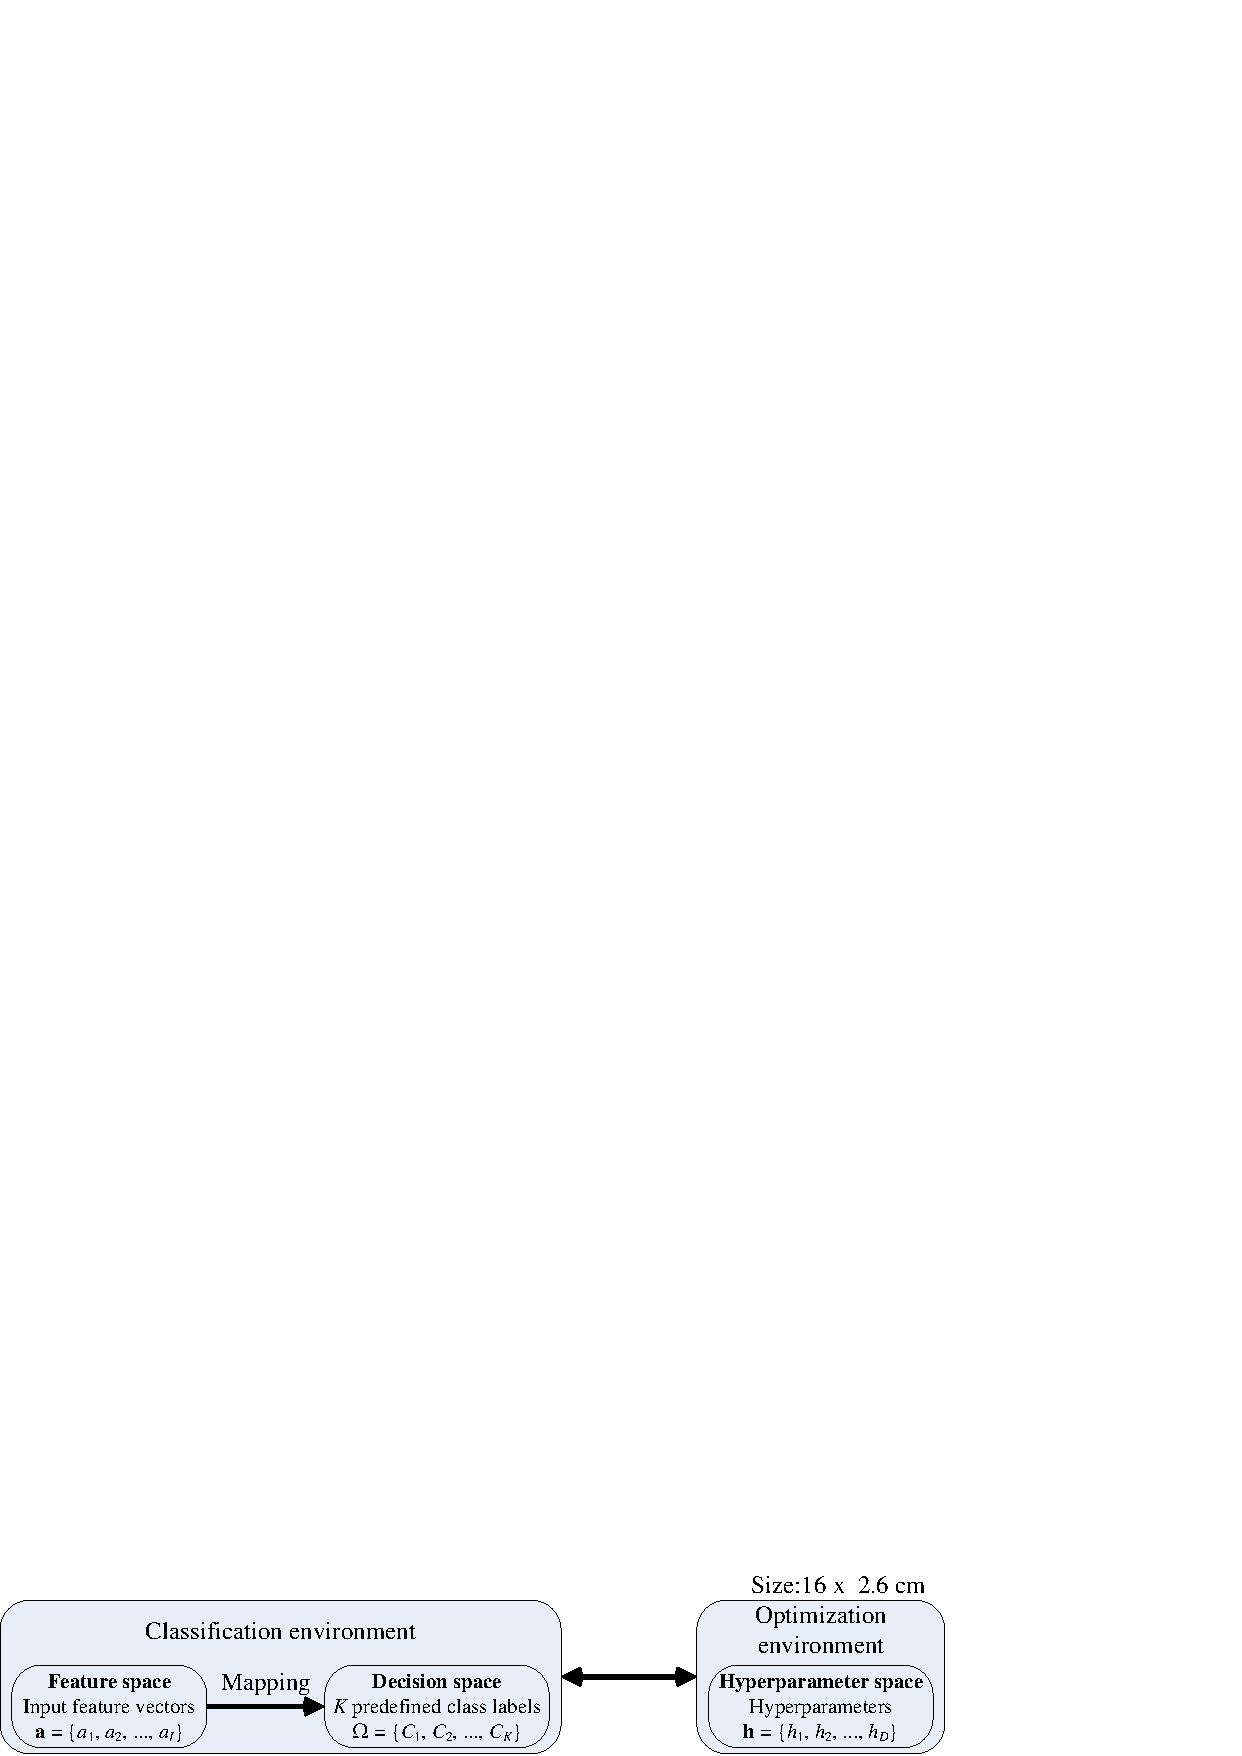
\includegraphics[width=0.9\linewidth, viewport=0cm 0cm 16.01cm 2.64cm, clip]
                  {c2_fig1}  }
  \caption{Pattern classification systems may be defined according to two environments.
A \emph{classification environment} that maps a $\mathbb{R}^I$ input feature space to a decision space, respectively defined by feature vectors \textbf{a}, and a set of class labels $\Omega$.
Interacting with the latter is an \emph{optimization environment}, where each vector \textbf{h} indicates a position in the hyperparameter space defined according a classifier's learning algorithm.
The representation space traversal seeks to maintaining diversity among classifiers by exploiting the interaction between these two environments.
The basic assumption is that different positions in the hyperparameter space lead to different class models in the feature space, and thus different class label $C_k$ predictions in the decision space}
	\label{fig:c2_environments}
\end{figure*}
%------------------------------- \Environments --------------------------------%

Diversity can be achieved via (1) different starting points in the input feature space, using a learning algorithm trained with different initial conditions, (2) different sets of accessible hypotheses using different training data sets (\emph{e.g.}, boosting and bagging) or different learning algorithms, and (3) representation space traversal that optimizes parameters, using a penalty term or evolutionary method, to ensure that base classifiers occupy different areas in the feature space.
In the latter case, the hyperparameters of a classifier (\emph{e.g.}, learning rate) define an optimization space (\cite{granger07}).
As described in Figure \ref{fig:c2_environments}, supervised learning strategies may then allow to optimize a classifier's hyperparameters such as accuracy is maximized.
Since these hyperparameters govern the learning dynamics of a classifier, diversity among solutions in the \emph{optimization environment} leads to ensemble diversity in the \emph{classification environment}.
Diversity can thus be maintained without relying on costly classifier diversity measures.

%-- Biometric / face recognition
The recognition of individuals based on their biometric traits provides a powerful alternative to traditional authentication schemes that are presently applied in security and surveillance systems.
In biometric applications, such as face recognition in video, the collection and analysis of labeled reference samples to design biometric systems (during an enrollment of re-enrollment process) is often expensive and time consuming.
Samples acquired from video streams in \emph{unconstrained} scenes are generally of poor quality with low resolution, resulting in classifiers applied to biometric matching that are often trained with limited and unbalanced data with much inter- and intra-class variability, 
Moreover, given that facial regions are often captured discreetly, without cooperation, they are subject to considerable variations due to limited control over operational conditions (\emph{e.g.}, illumination, pose, facial expression, orientation and occlusion).
In addition, operating conditions and individual physiology may even change over time, either temporary (\emph{e.g.}, haircut, glasses, lighting, etc.) or permanently (\emph{e.g.}, scars, aging).
New informations, such as input features and output classes, may suddenly emerge and previously acquired data may eventually become obsolete in dynamically changing classification environments (\cite{granger01, tsymbal08}).
These factors contribute to a growing divergence between the biometric model of an individual and its underlying class distribution.\footnote{Typically designed during an a priori enrollment phase, the biometric model of an individual for matching consists of one or more templates (reference samples) or the parameters statistical or structural model of reference samples.}

It is common in many biometric applications to acquire additional data and knowledge from the environment or other sources over time, after the system has originally been deployed for operations.
For accurate recognition of individuals, biometric systems should adapt their models over time in response to new or changing input features, data samples, priors, classes and environments.
In this chapter, it is assumed that new reference data becomes available to create new biometric models when individuals enroll to the system, and to update models of individuals previously enrolled to the system. 
Some adaptive biometric systems have been proposed in the literature to refine biometric models according to the intra-class variations in input samples (\cite{roli08}).
Indeed, with self-adaptive or semi-supervised learning strategies, biometric models are initially designed during enrollment using labeled training data, and then updated with highly confident unlabeled data obtained during operations (\cite{poh09, rattani10}).
These strategies are however vulnerable to outliers, dispersion and overlap in class distributions.
Stringent criteria are required for selection of highly confident data, to minimize the probability of introducing impostor data into updated biometric models.
In this chapter, supervised learning strategies are considered, and new data samples are assumed to be analyzed and labeled by an operator with expert knowledge of intra-class variations.
Labeled data becomes available, for instance, over multiple (re)enrollment sessions, or when operational scenarios are analyzed off-line, and can allow an operator to gradually build the biometric models of a system over time.
Adaptive biometric systems in literature have used newly-acquired reference samples to update the selection of a user's template from a gallery via clustering and editing techniques (\cite{uludag04}).
Others have performed on-line learning of genuine samples over time to update each user's single super template (\cite{jiang02}).
It is however difficult to represent intra-class variations with a single template (\cite{roli08}).

In previous work, the authors proposed an adaptive classification system (ACS) to update biometric models of individuals in response to new labeled reference data from the operational environment during video-based face recognition (\cite{connolly10}).
It uses the fuzzy ARTMAP (FAM) neural network for supervised incremental learning of limited data, as well as fast and efficient matching of facial regions detected in video streams against the model of individuals enrolled to a face recognition system.
The authors have showed that (1) adaptation of a FAM network during supervised incremental learning is a dynamic optimization problem in the hyperparameter space, and (2) corruption of the biometric models resulting from incremental learning of new data can be reduced using an ensemble-based approach (\cite{connolly10_2}).
It exist several directions to address uncertain classification environments with ensembles, such as changing classifier combination rules, updating classifiers using the new reference data, and changing ensemble structure by replacing old or underperforming members (\cite{kuncheva04}).
However, few of these approaches explicitly exploit classifier diversity when adapting ensembles over time in a context where to few data are available.

Given the limited amount of data available to design biometric systems, creating diversity among classifiers through \emph{representation space traversal} is an efficient way to exploit those data to provide reliable classifier ensembles.
For instance, with a cooperative neural network co-evolution paradigm (\cite{potter00}), evolutionary algorithms have been used to create \emph{heterogeneous} ensembles (\cite{valentini03}).\footnote{This definition differs with respect to certain other definitions of heterogeneous ensembles found in literature (\cite{oliveira09, rashid09}).}
It allows, exploring a hyperparameter space to train classifiers of the same type, on the same data, but with different learning dynamics.
These approaches, where classifiers cooperate, exchange information, but yet have their design and training be independent, have been shown to provide more accurate ensembles (\cite{bakker03, garcia05, liu01, zhou02}).

%-- Objective
In this chapter, the relationship between diversity in the classification and optimization environments is exploited for efficient design of heterogeneous ensembles of classifiers in video-based face recognition. 
Under the hypothesis that diversity in the hyperparameter space is correlated with diversity among a corresponding pool of classifiers in the feature and decision spaces, a specialized learning strategy based on dynamic particle swarm optimization (DPSO) is proposed for supervised incremental learning of new data.
This incremental DPSO-based learning strategy is applied to an adaptive multiclassifier system (AMCS) that consists of a pool FAM networks (\cite{carpenter92}) for classification that interacts with a niching version of DPSO (\cite{nickabadi08_2}).
The DPSO-based learning strategy incrementally evolves a heterogeneous ensemble of FAM networks in response to new reference data.
Each particle in the optimization environment corresponds to a FAM network in the classification environment, and the DPSO strategy cojointly optimizes \emph{all classifier parameters} -- hyperparameters, weights, and architecture -- of a pool of classifiers such as classification rate is maximized.
The ability of DPSO algorithms to find and track several changing local optima in the hyperparameter space is exploited by the AMCS to create a diversified pool (or swarm) of \emph{heterogeneous} classifiers.
DPSO properties are applied in a novel greedy search process to efficiently select an ensemble among the pool of FAM classifiers, based on accuracy and particle swarm diversity.

This study focuses on video-based face recognition applications in which two incremental learning scenarios may occur--enrollment and update of facial models.
Performance of this system is assessed in terms of classification rate and resource requirements for incremental learning of new data blocks from two real-world video data sets--Institute of Information Technology of the Canadian National Research Council (IIT-NRC) (\cite{gorodnichy05}) and Motion of Body (MoBo) (\cite{gross02}).
In proof-of-concept experiments, the AMCS performs biometric matching of facial regions against the facial model of individuals enrolled to a system for closed-set identification.
Finally, the relationship between diversity in a classifier's hyperparameter space and diversity in it's feature and decision space is analyzed for both batch and incremental learning cases.

%-- Structure
In Section \ref{sec:c2_adaptation}, the AMCS is described along with the FAM network used for classification, and the DPSO algorithm used to optimize system parameters.
In Section \ref{sec:c2_algo}, the new DPSO-based incremental learning strategy used to evolve heterogeneous ensembles is described.
Application, data bases, incremental learning scenarios, protocol, and performance measures used for proof-of-concept simulations are described in Section \ref{sec:c2_methodology}.
Finally, experimental results are presented and discussed in Section \ref{sec:c2_results_discussion}.

%--------------------------------- Adaptation ---------------------------------%
\section{An adaptive multiclassifier system}
\label{sec:c2_adaptation}

%------------------------- Framework - for section 2 --------------------------%
\begin{figure*}[t]
  \centering
  \fbox{
  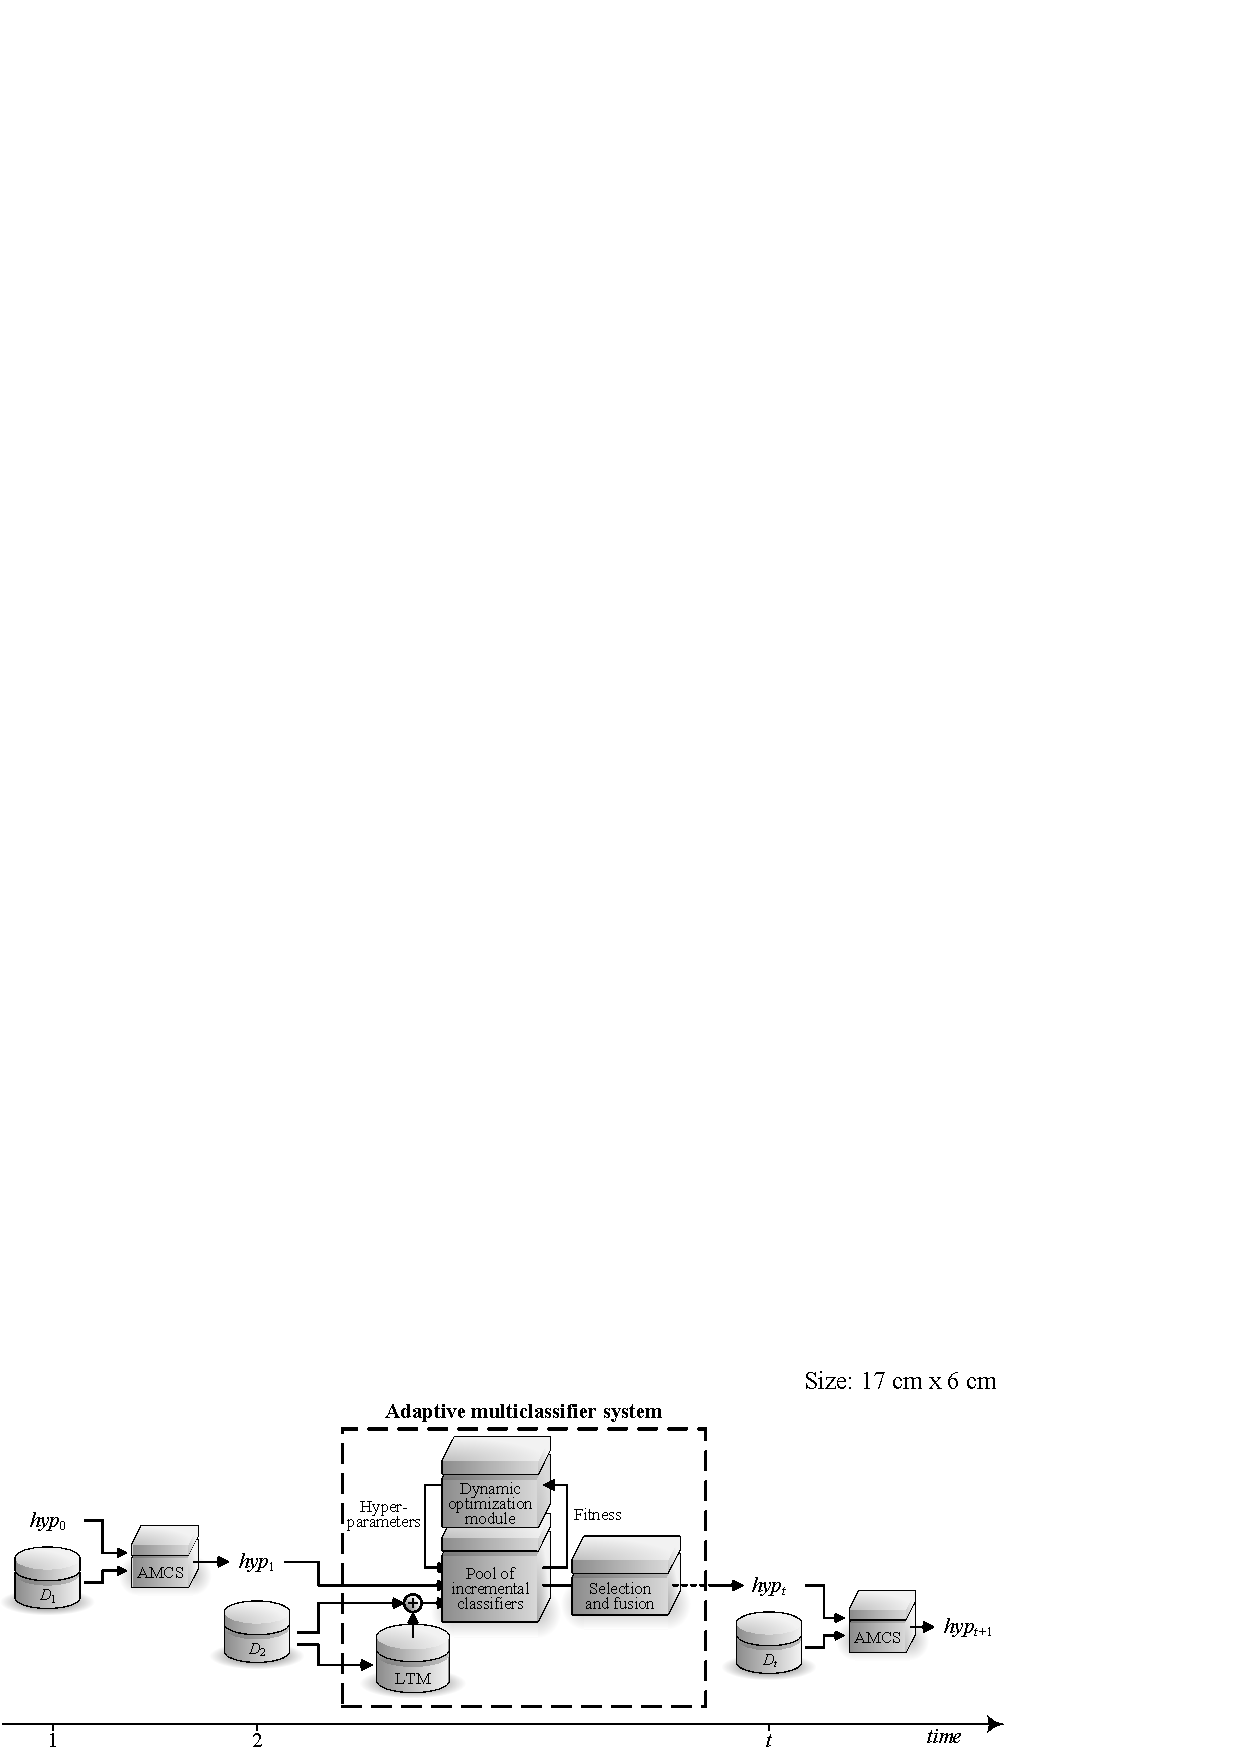
\includegraphics[width =0.97\linewidth, viewport =0cm 0cm 17cm 6cm, clip]
  								{c2_fig2} }
  \caption{Evolution over time of the adaptive multiclassifier system (AMCS) in a generic incremental learning scenario, where new blocks of data are used to update a swarm of classifiers.
Let $D_1$, $D_2$, ... be blocks of learning data that become available at different labeled instants in time $t=1,2,...,T$.
The AMCS starts with an initial hypothesis $hyp_0$ according to prior knowledge of the domain.
Each hypothesis $hyp_{t-1}$ are updated to $hyp_{t}$ by the AMCS on the basis of a new data blocks $D_t$}
	\label{fig:c2_framework}
\end{figure*}
%------------------------- \Framework - for section 2 -------------------------%

Figure \ref{fig:c2_framework} depicts the evolution of an adaptive multiclassifier system (AMCS) for supervised incremental learning of new reference labeled samples.
It is composed of a pool of base classifiers, each one suitable for supervised incremental learning, a dynamic evolutionary optimization module that tunes the user-defined hyperparameters of each classifier, and a long term memory (LTM) that stores and manages incoming data for validation.
This system differs from the system originally proposed in that a new DPSO incremental learning strategy allow to efficiently form a heterogeneous ensemble of classifiers (\cite{connolly10}).
It evolves a pool of classifiers, and is now composed of a selection and fusion module for efficient combination of heterogeneous ensembles.

When a new block of learning data $D_t$ becomes available to the system at a discrete time $t$, it is employed to update the LTM, and evolve the pool, or swarm, of incremental classifiers.
Each classifier is associated to a particle in the hyperparameter space, and a dynamic optimization module using a DPSO-based learning strategy cojointly determines the classifiers hyperparameters, architecture, and parameters such that classification rate is maximized (\cite{connolly10_2}).
Once the optimization process is complete, the selection and fusion module produces a heterogeneous ensemble by selecting and combining classifiers from the swarm, based on their accuracy and diversity.
The LTM stores data samples from each individual class for validation during incremental learning and fitness estimation of particles on the objective function (\cite{connolly10}).
The data from $D_t$ is partitioned and combined with that of the LTM to create three subsets: a training data set $D_t^\text{t}$, a validation data set $D_t^\text{v}$, and a fitness estimation data set $D_t^\text{f}$. 

In this chapter, a particular realization of this AMCS is considered.
The fuzzy ARTMAP (FAM) neural network (\cite{carpenter92}) is employed for incremental learning classification and a dynamical niching particle swarm optimization (DNPSO) algorithm (\cite{nickabadi08_2}) is used for dynamic optimization.
The rest of this section provides additional details on the FAM classifier and the DNPSO algorithm used within the AMCS.

%------------------------------------------------------------------------------%
%------------------------- Subsection : fuzzy ARTMAP --------------------------%
\subsection{Fuzzy ARTMAP neural network classifiers}
\label{sec:c2_fam}

Fuzzy ARTMAP (\cite{carpenter91}) is a versatile neural classifier that may provide a high level of prediction accuracy with moderate time and memory complexity (\cite{granger07}).
As such, fuzzy ARTMAP has been successfully applied to a wide variety of pattern recognition problems.
It is very promising for fast and efficient for biometric matching (of feature patterns against the model of individuals enrolled to a face recognition system) due to its ability to perform fast, stable, on-line, unsupervised or supervised, and incremental learning from limited amount of training data. 
A key feature of the ARTMAP networks is their unique solution to the stability-plasticity dilemma.
The popular fuzzy ARTMAP integrates the fuzzy ART to process both analog and binary-valued input patterns to the original ARTMAP architecture (\cite{carpenter92}).
Several other ARTMAP networks have been proposed to address this architecture to specific problems.
Members of the ARTMAP family can be broadly divided according to their internal matching process, which depends on either deterministic or probabilistic category activation (\cite{connolly09}).

%-------------------------------- Fuzzy ARTMAP --------------------------------%
\begin{figure*}[!t]
  \centering
  \fbox{
  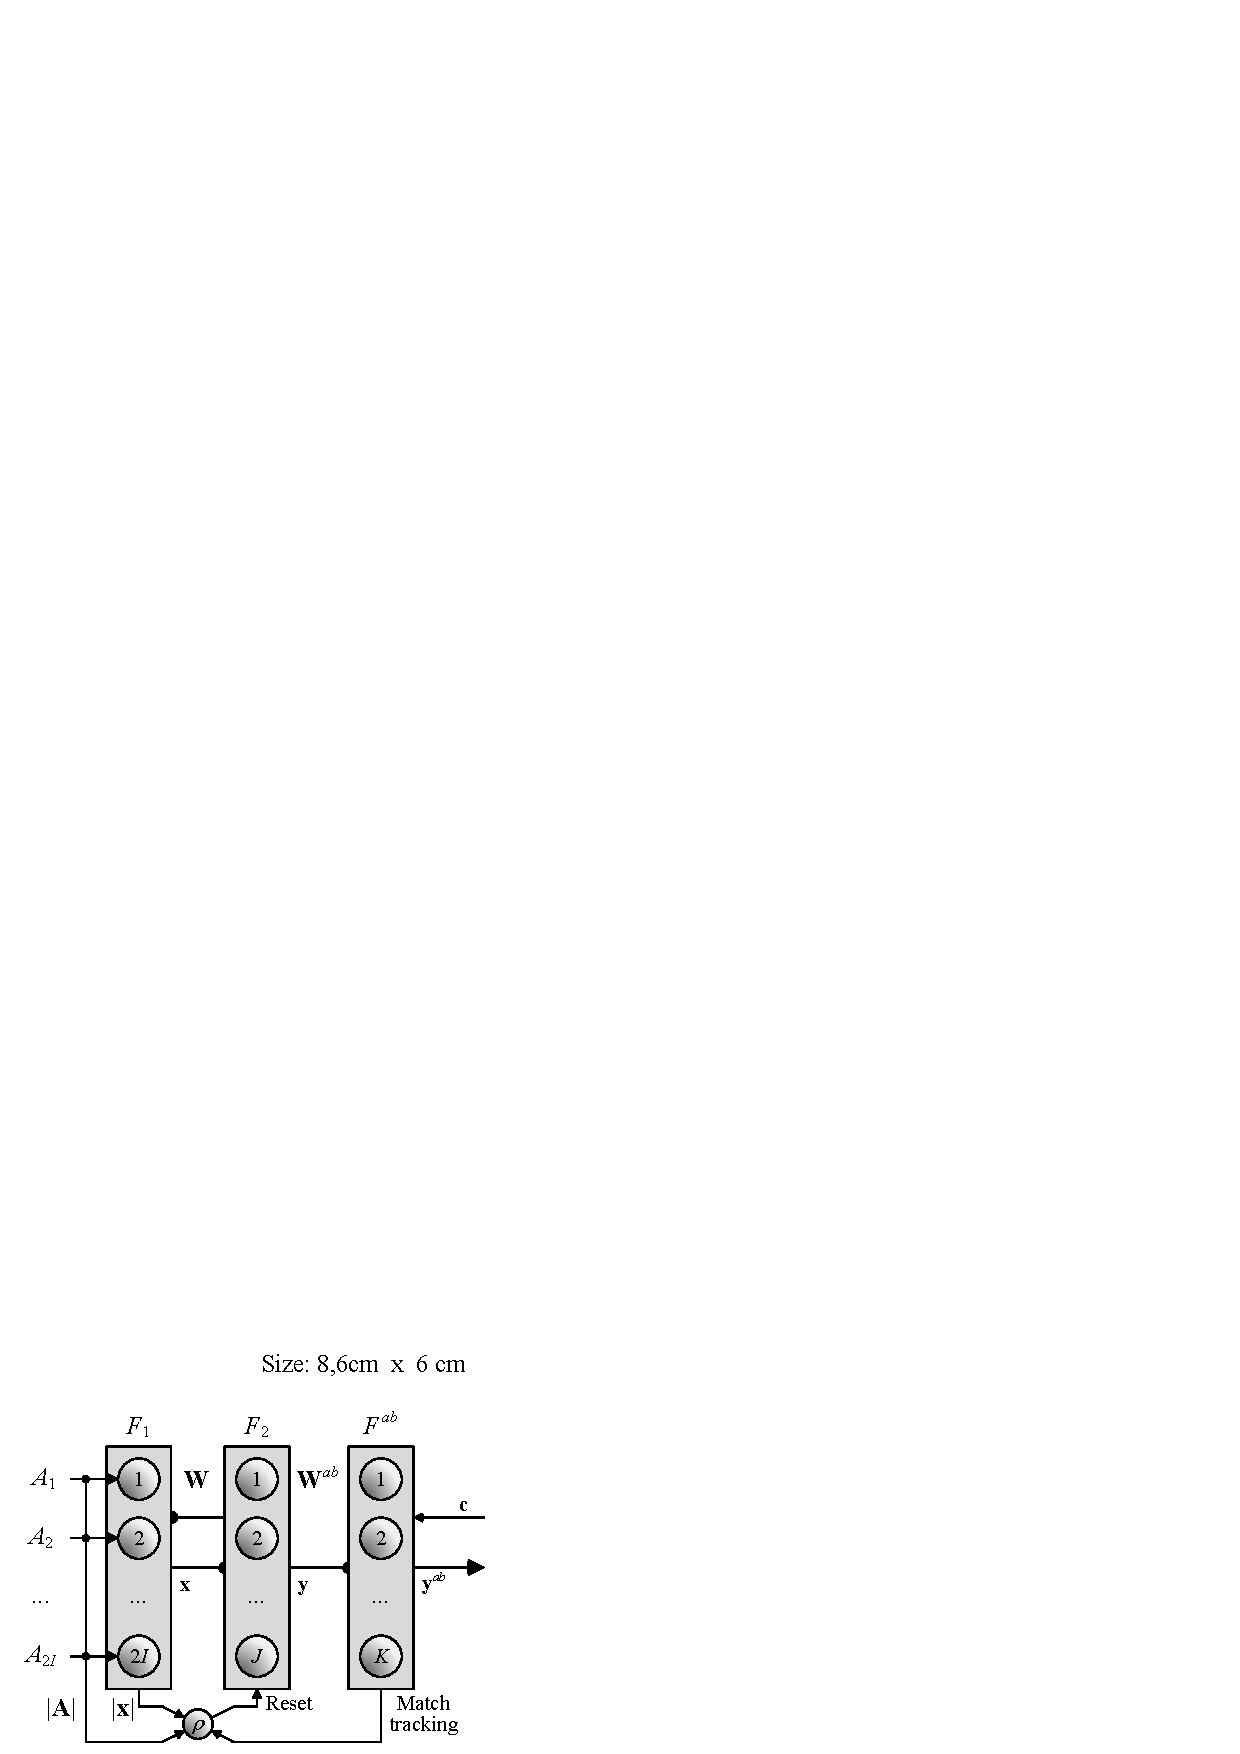
\includegraphics[width=0.5\linewidth, viewport=0cm 0cm 8.6cm 6cm, clip]
  							  {c2_fig3} }
	\caption{Fuzzy ARTMAP neural network}
	\label{fig:c2_fam}
\end{figure*}
%------------------------------- \Fuzzy ARTMAP --------------------------------%

As shown in Figure \ref{fig:c2_fam}, the fuzzy ARTMAP (FAM) architecture consists of three layers: (1) an input layer $F_1$ of $2I$ neurons, with two neurons associated with each input feature (in $\mathbb{R}^I$), (2) a competitive layer $F_2$ of $J$ neurons, each one associated to a recognition category in the feature space, and (3) a map field $F^{ab}$ of $K$ output neurons, each one corresponding to a class (\cite{carpenter92}).

In supervised training mode, FAM learns an arbitrary mapping between training set patterns $\textbf{a}$ = $(a_1, a_2, ..., a_I)$ and their corresponding binary supervision patterns $\textbf{c}$ = $(c_1, c_2, ..., c_K)$.
These patterns are coded to have the value $c_k = 1$ if $k^*$ is the target class label for $\textbf{a}$, and zero elsewhere.
Components of the vector $\textbf{a}$ are scaled so that each $a_i \in [0,1]$, for $i=1 \ldots I$.
Complement coding doubles the number of components in the input vector, which becomes $\textbf{A} \equiv (a_1, a_2, ..., a_I, 1-a_1, 1-a_2,..., 1-a_I)$.
The prototype vector $\textbf{w}_{j} = (w_{1j}, ..., w_{2Ij})$, linking each $F_1$ input node to $F_2$ node $j$, may be visualized as a hyper-rectangle in the $\mathbb{R}^I$ feature space defined by all the input vectors $\textbf{a}$ that selected node $j$ during training.
Binary weight vectors $\textbf{w}^{ab}_{j} = (w_{j1}, ..., w_{jK})$ connects $F_2$ nodes to one of the $K$ classes of $F^{ab}$.

Initially, all the $F_2$ nodes are uncommitted, all weight values $w_{ij}$ are initialized to 1, and all weight values $w^{ab}_{jk}$ are set to 0.
Prior processing each new training pattern $\textbf{a}$, the vigilance parameter is set: $\rho=\bar{\rho}$.
Given an input $\textbf{a}$ and supervision output $\textbf{c}$, the coding field $F_2$ is activated according to the Weber law choice function:
\begin{equation}
	T_j(\textbf{A}) = |\textbf{A}\wedge\textbf{w}_{j}| / (\alpha + 			
										|\textbf{w}_{j}|),
	\label{eq:choice}
\end{equation}
where $(\textbf{p}\wedge\textbf{q})_i \equiv \textrm{min} (p_i,q_i)$, $|\textbf{p}| \equiv \sum^{2I}_{i=1} |p_i|$, and $\alpha$ is the \emph{choice parameter}.
With winner-take-all coding, the $F_2$ node $j^*$ that receives the largest activation $T_{j^*}(\textbf{A})$ is chosen, and undergoes the vigilance test defined by: 
\begin{equation}
	|\textbf{A}\wedge\textbf{w}_{j^*}| / |\textbf{A}|=|\textbf{A} \wedge 
		\textbf{w}_{j^*}|/I > \rho,
	\label{eq:match}
\end{equation}
where $\rho \in [0,1]$ is the dimensionless \emph{vigilance parameter}.
If node $j^*$ passes the vigilance test, FAM predicts the class corresponding to $j^*$.
If the prediction is correct (\emph{i.e.}, $k(j^*)=k^*$), weight vector $\textbf{w}_j$ undergoes learning and is adjusted according to
\begin{equation}
  \textbf{w}_{j^*}' = \beta(\textbf{A} \wedge \textbf{w}_{j^*}) + 
   										(1 - \beta) \textbf{w}_{j^*} \,,
  \label{eq:learning}
\end{equation}
where $\beta \in [0,1]$ is a fixed \emph{learning rate parameter}.

If neuron $j^*$ does not pass the vigilance test, or makes an \emph{incorrect} class prediction, it is deactivated for the rest of the search process with the current input $\textbf{a}$.
When an incorrect class prediction occurs, a \emph{match tracking} signal also adjusts vigilance such as $\rho = |\textbf{A} \wedge	\textbf{w}_{j^*}|/I + \epsilon$, where $\epsilon$ is the match tracking parameter.\footnote{In this chapter, negative match tracking is employed (\cite{carpenter98}).}
The network then searches for another $F_2$ node that either satisfies both requirements, or commits a new $F_2$ node to encode $\textbf{a}$ if no such node exist.
When a new $F_2$ node is committed, network size is actualized ($J=J+1$), and the last committed node learns the correct output class by setting  $\textbf{w}_J = \textbf{A}$ and $w^{ab}_{Jk^*} = 1$.

During training, FAM internal dynamics are governed by four hyperparameters: the choice parameter $\alpha \geq 0$, the learning parameter $\beta \in [0,1]$, the match tracking parameter $\epsilon \in [-1,1]$, and the baseline vigilance parameter $\bar{\rho} \in [0,1]$.
Let $\textbf{h}=(\alpha, \beta, \epsilon, \bar{\rho})$ be defined as the vector of FAM hyperparameters, these are inter-related and each have a distinct impact on network dynamics.
While $\alpha$ and $\epsilon$ determine the depth of search attained before an uncommitted node is selected, and $\bar{\rho}$ limits the maximal size of the category hyper-rectangles in the $\mathbb{R}^I$ feature space.
Although this is affected by the match tracking signal $\epsilon$, low baseline vigilance generally results in large hyper-rectangles and leads to broad generalization and abstract memories, while high vigilance yields small hyper-rectangles, leading to narrow generalization and detailed memories.
During learning, $\beta$ determines the speed with which the recognition categories expand to fit $\textbf{a}$.
The algorithm can be set to slow learning with $0<\beta<1$, or to fast learning with $\beta=1$.
With fast learning, each hyper-rectangles is just large enough to enclose the training set patterns $\textbf{a}$ to which it has been assigned.
Prototype vector $\textbf{w}_j$ records the largest and smallest component values of training subset patterns $\textbf{a}$ assigned to category $j$.

A standard vector of hyperparameters $\textbf{h}_\text{std} = (\alpha = 0.001, \beta=1, \epsilon=0.001, \bar{\rho}=0)$ is commonly fixed to minimize network complexity (\cite{carpenter92}).
However, Figure 4 illustrates with a synthetic 2D data base (\cite{valentini03}) that adjusting these hyperparameters allows to adapt FAM learning dynamics with regards to currently available training data.
By using different hyperparameters settings to train FAM, each network learns different hyper-rectangles to fit the same data, leading to different decision boundaries and predictions.
This diversity of opinion among classifiers may then be measured using several different indicators (\cite{canuto07, hadjitodorov06, kapp07, oliveira09, sirlantzis08, ulas09}).

It is very well known that ensembles of classifiers can be used to improve the generalization capabilities of pattern recognition systems applied in different domains, including face recognition in video (\cite{er02, lu06, su07}).
But as Figure 4 shows, varying the hyperparameter values of several FAM neural networks provides an easy mean to model the same data with different perspective and generate a diversified pool of heterogeneous classifiers when few learning reference data is available. 
Given this correlation between diversity of hyperparameter values and decision boundaries, classifier diversity can also be easily exploited during ensemble selection form the pool to further improve accuracy of the face recognition system (\cite{brown05}).

%-------------------------- P2 data & FAM boundaries --------------------------%
\begin{figure*}[t]
  \centering
  \fbox{
		\subfloat[Original data]{
		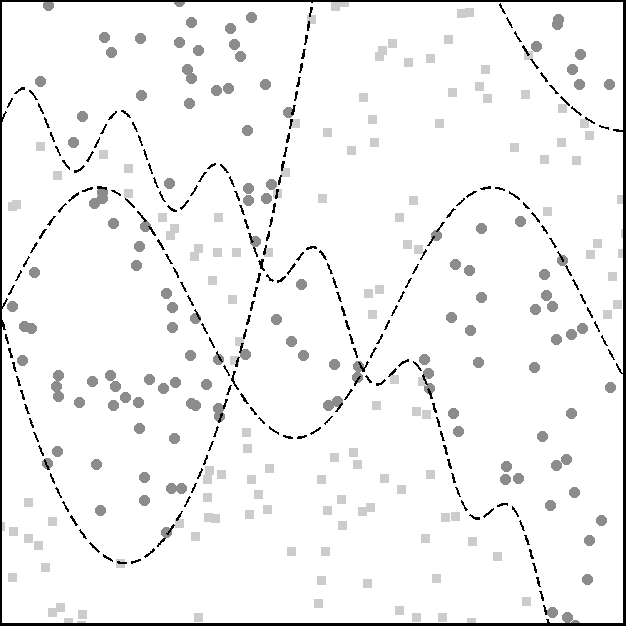
\includegraphics[width=0.22\linewidth]{c2_fig4a} \label{fig:c2_dbp2} }
		\quad
		\subfloat[FAM decision boundaries]{
			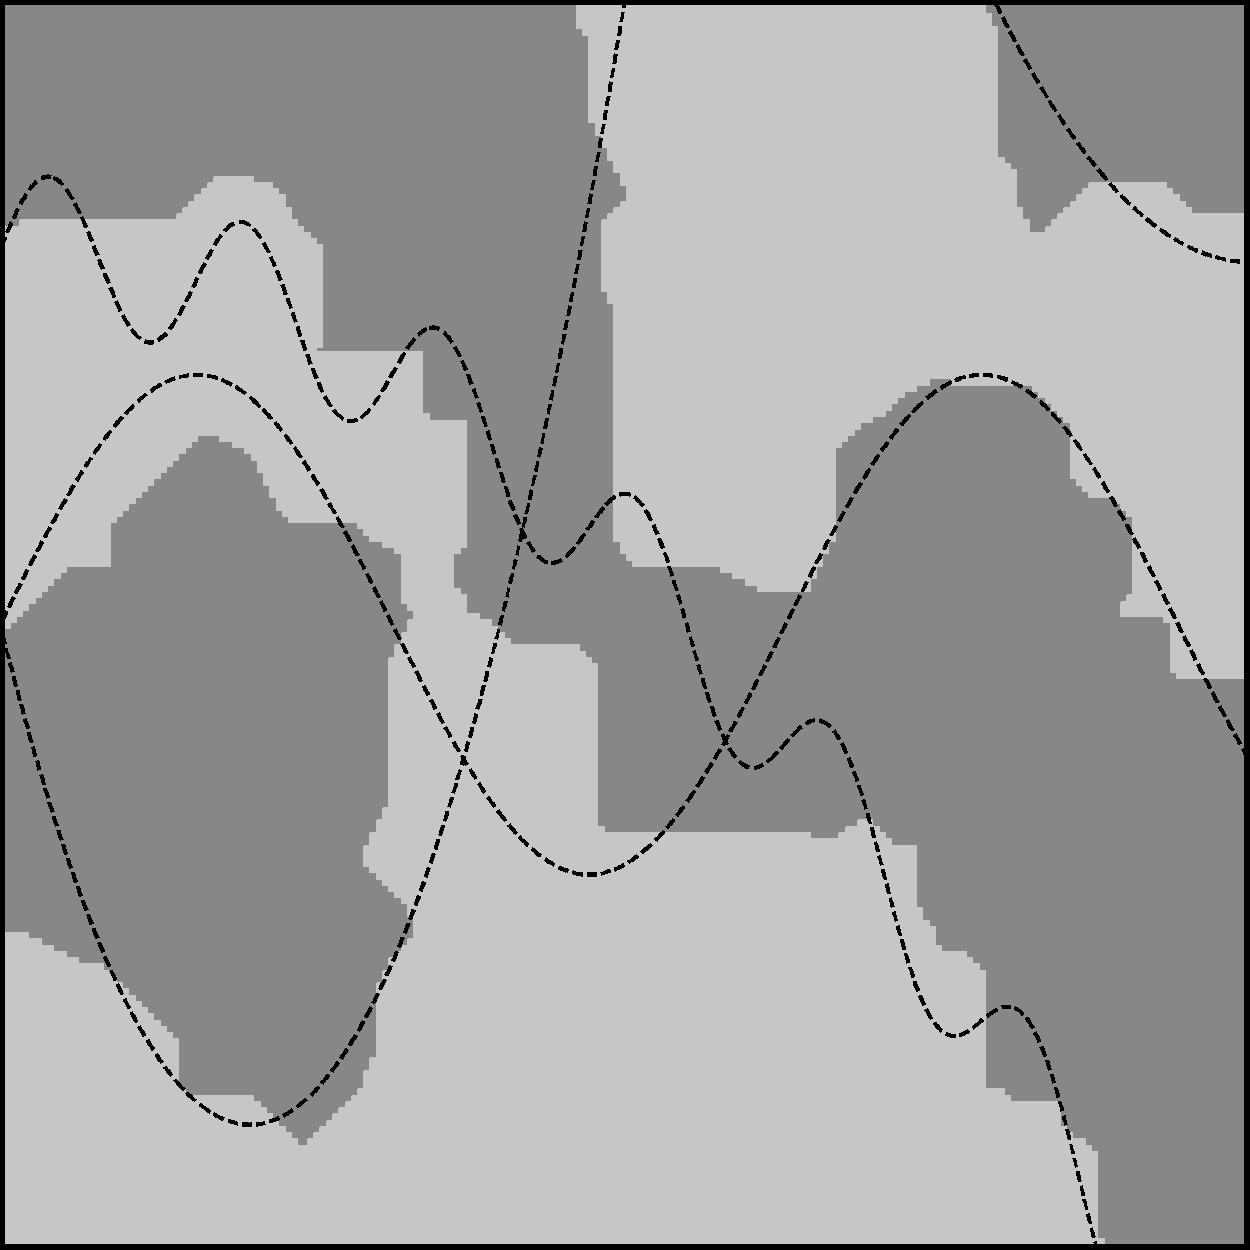
\includegraphics[width=0.22\linewidth]{c2_fig4b} 
			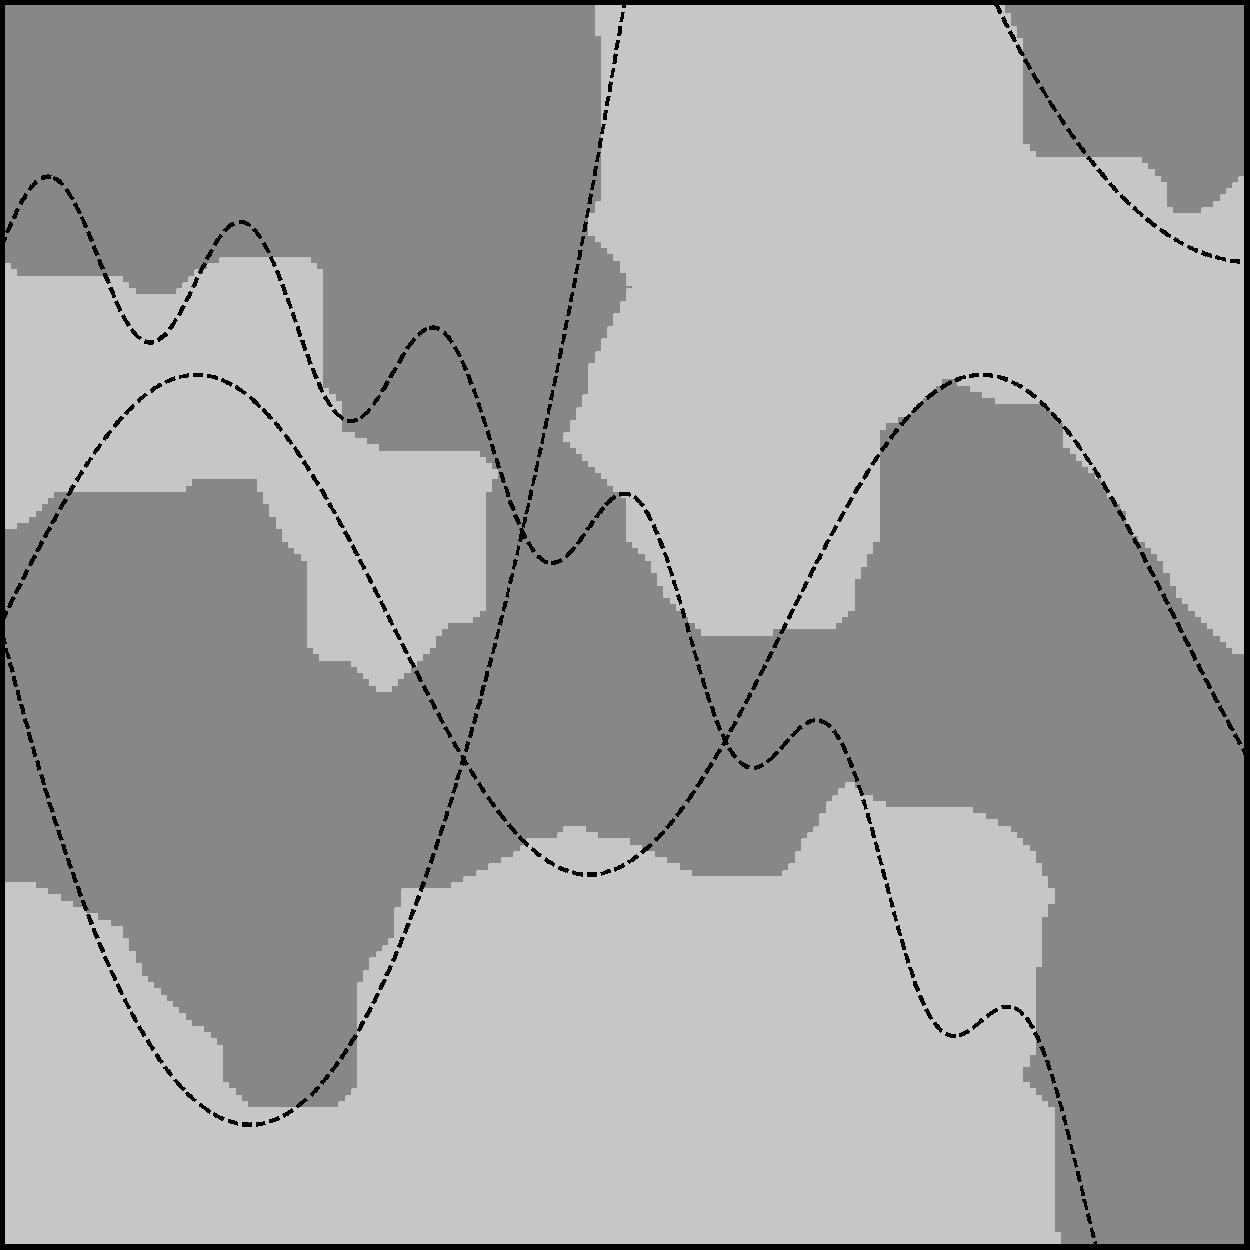
\includegraphics[width=0.22\linewidth]{c2_fig4c} 
			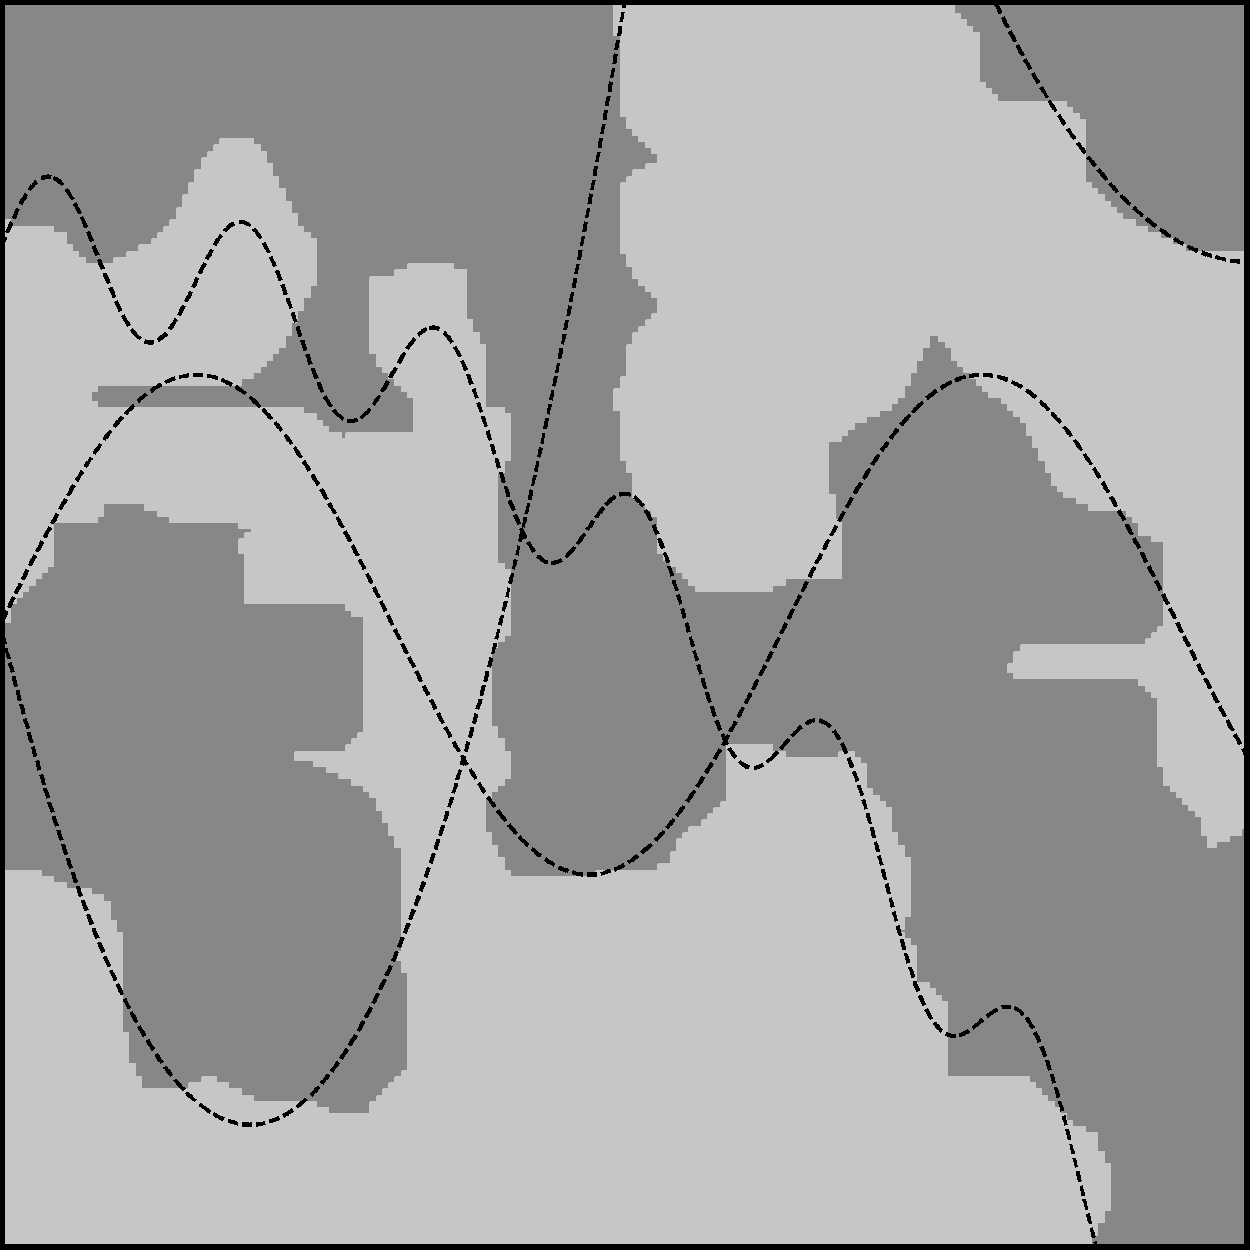
\includegraphics[width=0.22\linewidth]{c2_fig4d}
			\label{fig:c2_famBound}
		}
	}
  \caption{Training data (\ref{fig:c2_dbp2}) from the P2synthetic data base (\cite{valentini03}), and decision boundaries for FAM trained with different hyperparameters that are respectively (\ref{fig:c2_famBound}): $\textbf{h}=($70, 0.70, 0.80, 0.85), $\textbf{h}=($13, 0.41, 0.08, 0.86), and $\textbf{h}=($67, 0.73, 0.68, 0.89)}
	\label{fig:c2_bound}
\end{figure*}
%------------------------- /P2 data & FAM boundaries --------------------------%

%------------------------------------------------------------------------------%
%------------------------------ subsection : pso ------------------------------%
\subsection{Dynamic particle swarm optimization}
\label{sec:c2_dpso}

Particle swarm optimization (PSO) is a population-based stochastic optimization technique that was inspired by social behavior of bird flocking and fish schooling.
With PSO, each particle corresponds to a single solution in the hyperparameter space, and the population of particles is called a swarm.
Particles move through the hyperparameter space and change their course under the guidance of a cognitive influence (i.e., their own previous search experience) and a social influence (i.e., their neighborhood previous search experience).
Unlike evolutionary algorithms (like genetic algorithms), each particle always stores its best position and the best position of its surroundings in its memory.

Originally developed for static optimization problems, the PSO algorithm has been adapted for dynamic optimization problems by adding mechanisms to (1) modify the social influence to maintain diversity in the optimization space and detect several optima, (2) detect changes in the objective function by using the memory of each particle, and (3) adapt the memory of its population if change occur in the optimization environment.
The latest particle swarm optimization algorithms developed to insure diversity in the swarm are presented in \cite{du08, li06, nickabadi08_2, ozcan07}.
Change detection and memory adjustment mechanisms for DPSO are presented in \cite{blackwell04, carlisle02, hu02, wang07}.

During supervised incremental learning of new data blocks $D_t$, the dynamic optimization module (see Figure 2) iteratively updates the hyperparameter vector $\textbf{h}=\left(\alpha, \beta, \epsilon, \bar{\rho}\right)$ of each FAM classifier in the hyperparameter space, and determines the position $\textbf{h}$ such that the FAM classification rat is maximized.
In this chapter, the hyperparameter space is bounded by $\alpha \in \left[0,100\right]$, $\beta \in \left[0,1\right]$, $\epsilon \in \left[-1,1\right]$, and $\bar{\rho} \in \left[0,1\right]$.
Using PSO to evolve a swarm of FAM networks when data is learned incrementally over time, such adaptation has been shown to correspond to a dynamic optimization problem defined by  
\begin{equation}
	\textnormal{maximize }\{ f(\textbf{h},t)\ |\ \textbf{h}\in\mathbb{R}^4,
																             \ t\in\mathbb{N}_1 \},
	\label{eq:optDyn}
\end{equation}
where the fitness, $f(\textbf{h},t)$, is the FAM classification rate for a given vector of hyperparameters $\textbf{h}$, and after learning data set $D_t$ at a discrete time $t$ (\cite{connolly10}).
There are three different types of dynamic optimization environment (\cite{engelbrecht05}): type I, where the location of the optimum changes over time; type II, where the location of the optimum remains fixed, but the value of the objective function optimum's position changes; and type III, where both the location and value of the optimum position change.
In \cite{connolly10}, it was shown that the optimization problem defined by Equation \ref{eq:optDyn} constitute a type III optimization environment.

%-------------------- DNPSO - subswarms and free particles --------------------%
\begin{figure*}[t]
  \centering
  \fbox{
		\subfloat[$t=1$]{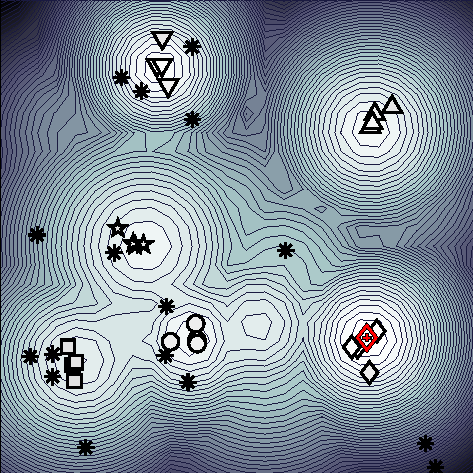
\includegraphics[width=0.23\linewidth]{c2_fig5a}}
		\hspace{1mm}
		\subfloat[$t=2$]{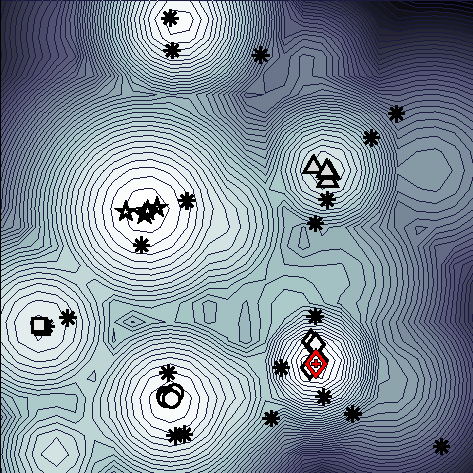
\includegraphics[width=0.23\linewidth]{c2_fig5b}}
		\hspace{1mm}
		\subfloat[$t=3$]{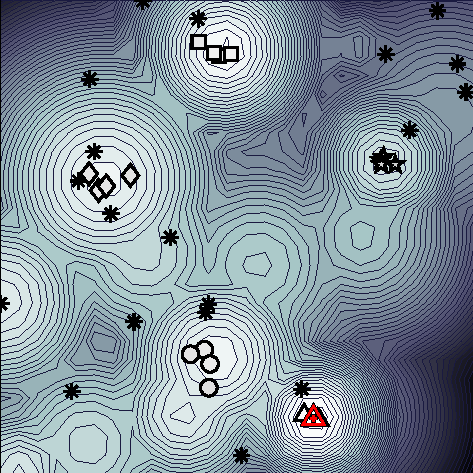
\includegraphics[width=0.23\linewidth]{c2_fig5c}}
		\hspace{1mm}
		\subfloat[$t=4$]{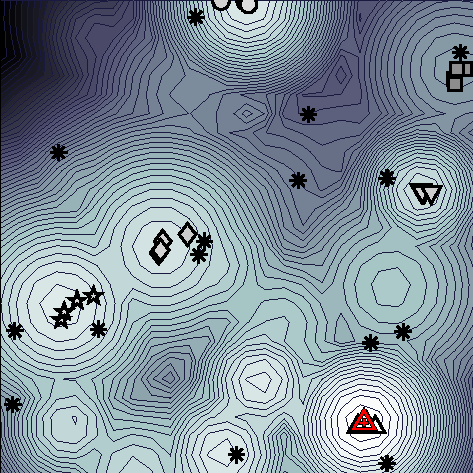
\includegraphics[width=0.23\linewidth]{c2_fig5d}}
	}
	\caption{Evolution of DNPSO particles for different changes in a type III 
optimization environment using the 2D multipeak benchmark problem (\cite{branke99}).
In a video-based face recognition application for instance, this could be the classification rate landscape in a 2D hyperparameter space.
Subswarms (shapes: circle, rectangle, etc.) are created dynamically around the \emph{masters} -- particles that detected local optima.
Subswarms converge toward the local optima detected for the objective function.
Free particles (stars), that are not associated to any subswarms, are free to explore the optimization space using only their cognitive influence.
At different times $t$, the personal best of each particles is reevaluated to accommodate changes that may occur on the objective function}
	\label{fig:c2_dnpso}
\end{figure*}
%------------------- /DNPSO - subswarms and free particles --------------------%

In this chapter, the adaptive multiclassifier system (AMCS) employs the Dynamical Niching PSO (DNPSO) algorithm (\cite{nickabadi08_2}) to maximize FAM classification rate as a function of its hyperparameters.
As depicted in Figure \ref{fig:c2_dnpso}, this algorithm maintains diversity in the hyperparameter search space by (1) using a local neighborhood topology, where subswarms are dynamically created around \emph{masters} (particles that are their own local best in their neighborhood), by (2) defining a minimal distance within which two masters that cannot co-exist, by (3) allowing free particles that do not belong to a subswarm, to move independently, and by (4) reinitializing those free particles that exhibit low velocities, indicating that they have converged on a non-optimal position.
DNPSO has also been adapted for dynamic optimization problems by updating the fitness of the best position of each particle at each iteration.
Using the moving peaks benchmark, the DNPSO algorithm has been shown to detect local optima and converge toward the global maximum in a multimodal type III optimization environment (\cite{nickabadi08_2}) (see Figure \ref{fig:c2_dnpso}).

When evolving FAM neural networks, updating the fitness of the best position of each particle at each iteration would double the number of time each network are trained, leading to a very costly process.
However, for an AMCS, changes in the objective function may only occur when a new data block $D_t$ becomes available.
Thus, the best position's fitness of each particle is only updated when a new $D_t$ is presented to the system, \emph{before} the iterative DNPSO process.

%------------------------------------------------------------------------------%
%------------- subsection: Heterogeneous Ensemble of FAM Networks -------------%
\section{Strategy for evolving heterogeneous ensemble of FAM networks}
\label{sec:c2_algo}

The DPSO-based incremental learning strategy proposed in this chapter is based on the hypothesis that maintaining diversity among particles in the optimization environment implicitly generates diversity among classifiers in the classification environment.
By associating each classifier of a pool to a particle in a swarm, properties of a DPSO algorithm (to maintain diversity in the hyperparameter space) may be exploited to evolve a diversified heterogeneous ensembles of FAM networks over time, as new data becomes available.

This section describes the DPSO-based incremental learning strategy used to evolve heterogeneous ensembles of classifiers in response to new labeled reference samples.
First, a diversified pool of FAM networks is generated and evolved according to a DPSO learning algorithm (Section \ref{sec:c2_pool}).
This pool (or swarm) allows for efficient selection and fusion of ensembles of classifiers based on FAM accuracy and particle swarm diversity in the hyperparameter space (Section \ref{sec:c2_sel}).


%--------------------- subsection: DPSO learning strategy ---------------------%
\subsection{Generation and evolution of heterogeneous classifier pools}
\label{sec:c2_pool}

Algorithm \ref{alg:c2_pso} describes the DPSO algorithm proposed to generate and evolve a diversified pool (or swarm) of $N$ FAM networks.
During incremental learning of a data block $D_t$, their hyperparameters, parameters and architecture are cojointly optimized such that the classification rate is maximized.
For a PSO algorithm with $n=1, ..., N$ particles, each a hyperparameter vector (noted $\textbf{h}_n$), a total of $2N+1$ FAM networks is required.
The system stores $n=1, ..., N$ networks $\textit{FAM}_n^\text{start}$ in a short term memory to preserve networks associated with the best position of each particle (noted $\textbf{h}^*_n$) at time $t-1$.
It also stores $\textit{FAM}_n$, the model associated with $\textbf{h}^*_n$ during the optimization process at time $t$, and $\textit{FAM}_\text{est}$, a network employed for fitness estimation.
To minimize the impact of pattern presentation order at a time $t$, FAM networks are trained using the training data set $D_t^\text{t}$ under five different random pattern presentation orders.
To determine the number of training epochs, cross-validation is performed with the validation data set $D_t^\text{v}$, while fitness is estimated using the fitness estimation data set $D_t^\text{f}$ (\cite{connolly10}).
Overall fitness is defined as the highest classification rate achieved over the five pattern presentation orders, and $\textit{FAM}_\text{est}$ is the network that yields this highest classification rate.

%------------------------------ Algorithm : pso -------------------------------%
\begin{algorithm*}[t]
	\caption{DPSO learning algorithm}
	\label{alg:c2_pso}
 	\fbox{\begin{minipage}{0.97\linewidth}\centering
	\begin{algorithmic}[1]
		\Require New data sets $D_t$ for learning.
		\Ensure  Pool (or swarm) of $N$ FAM networks $\textit{FAM}_n$.
						
		\Statex\vspace{6pt}\textbf{Initialization:}\vspace{3pt}
		\State  $\bullet$ Set the swarm's parameters,                             
		\Statex $\bullet$ Initialize all $N$ networks $\textit{FAM}_{n}$ and
					 					  $\textit{FAM}_n^\text{start}$,
		\Statex	$\bullet$ Set PSO iteration counter at $\tau=0$, and              
		\Statex	$\bullet$ Randomly initialize particles positions and velocities. 
					 																									\label{l:c2_init}
		%-- For each learning block
		\Statex\vspace{9pt}\textbf{Upon reception of a new data block $D_t$, the
					 following incremental process is initiated:}\vspace{3pt}
					 
			%-- Personal best update
			\Statex\textit{Update the fitness of networks associated to the 
						  personal best positions:}\vspace{3pt}
			
			\For{ each particle $n$, where $ 1 \leq n \leq N$ }		\label{l:c2_pUpdate}
				\State Train and validate $\textit{FAM}_n$ with $D_t^\text{t}$ and
				       $D_t^\text{v}$ respectively, and estimate $f(\textbf{h}^*_n, t)$ 
				       using $D_t^\text{f}$.			                \label{l:c2_trnUpdate}
			\EndFor                                            \label{l:c2_endpUpdate}
			
			%-- Loop iterations
			\Statex\vspace{6pt}\textit{Optimization process:}\vspace{3pt}
			\While{ PSO does not reach stopping condition }						\label{l:c2_opt}
				\State Update particle positions according to the DNPSO algorithm.			
																														\label{l:c2_newPos}
				\For{each particle $n$, where $ 1 \leq n \leq N$}		\label{l:c2_fUpdate}
					\State $\textit{FAM}_\text{est}$ $\leftarrow$   \label{l:c2_famUpdate}
								 $\textit{FAM}_n^\text{start}$
					\State Train $\textit{FAM}_\text{est}$ with validation using
								 $D_t^\text{t}$ and $D_t^\text{v}$, and estimate
								 $f(\textbf{h}_n(\tau),t)$ using $D_t^\text{f}$.
								 																						\label{l:c2_trnOpt}
					\If{ $f(\textbf{h}_n(\tau),t) > f(\textbf{h}^*_n,t)$ }																																						\label{l:c2_ifNewP}
						\State \{$\textbf{h}^*_n$, $\textit{FAM}_n$,
										 $f(\textbf{h}^*_n,t)$\} $\leftarrow$ 
									 \{$\textbf{h}_n(\tau)$, $\textit{FAM}_\text{est}$,
									   $f(\textbf{h}_n(\tau),t)$\}				 \label{l:c2_pAssign}
					\EndIf 																				 \label{l:c2_endifNewP}
				\EndFor																					 \label{l:c2_endfUpdate}
				\State $\tau = \tau + 1$											 	 \label{l:c2_itUpdate}
			\EndWhile 																				 \label{l:c2_endOpt}

			\Statex\vspace{6pt}\textit{Define initial conditions for fitness
						 estimation with $D_{t+1}$:}\vspace{3pt}
			\For{ each particle $n$, where $ 1 \leq n \leq N$ }		\label{l:c2_sUpdate}
				\State $\textit{FAM}_n^\text{start}$ $\leftarrow$ $\textit{FAM}_n$
			\EndFor																						\label{l:c2_endsUpdate}
	\end{algorithmic}
	\end{minipage} }
\end{algorithm*}
%------------------------------------------------------------------------------%

During the initialization process (line \ref{l:c2_init}), all the FAM networks are initialized, and the swarm's parameters are set.
Particle positions are then randomly initialized within their allowed range.
When a new $D_t$ becomes available, the optimization process begins.
Fitness associated with the best position of each particle, $f(\textbf{h}^*_n,t)$, is updated according to the new data along with each network $\textit{FAM}_n$ (lines \ref{l:c2_pUpdate}--\ref{l:c2_endpUpdate}).
The optimization process continues were it previously ended until the DNPSO algorithm converges (lines \ref{l:c2_opt}--\ref{l:c2_endOpt}).
The DNPSO algorithm changes the position of subswarms and free particles in the hyperparameter space, and iteratively update each particle's new position along with their fitness (lines \ref{l:c2_newPos}--\ref{l:c2_endfUpdate}).
If new personal best positions are found, the position ($\textbf{h}^*_n$), fitness ($f(\textbf{h}^*_n,t)$), and network associated with the personal best $\textit{FAM}_n$ are updated (lines \ref{l:c2_ifNewP}--\ref{l:c2_endifNewP}).
At each iteration $\tau$, in the cases of equality between $f(\textbf{h}_n(\tau),t)$ and $f(\textbf{h}^*_n,t)$, the network that requires the least resources ($F_2$ nodes) is kept.
Finally, the iteration counter $\tau$ is incremented (line \ref{l:c2_itUpdate}).

Once the DNPSO algorithm converges, the $\textit{FAM}_n$ networks associated to each personal best are stored as $\textit{FAM}_n^\text{start}$ (lines \ref{l:c2_sUpdate}--\ref{l:c2_endsUpdate}).
These networks provide a short term memory of the swarm's state after learning data block $D_{t}$.
When new data becomes available at a time $t+1$, the best network previously obtained at time $t$ ($\textit{FAM}_n^\text{start}$) serves as the initial condition, and is copied to $\textit{FAM}_\text{est}$ prior training on $D_{t+1}$ each time the fitness of particle $n$ is estimated.
For the first learning block $D_1$, the $\textit{FAM}_n^\text{start}$ networks are in an initial state (see Section \ref{sec:c2_fam}).

%--------------------- subsection: Ensemble selection ----------------------%
\subsection{Selection of diversified ensembles}
\label{sec:c2_sel}

Once the pool of classifiers has evolved (Algorithm \ref{alg:c2_pso}), members of this pool are selected to form a heterogeneous ensemble, where each network is trained on the same data, but with different hyperparameters (\cite{valentini03}).
In Algorithm \ref{alg:c2_ens}, DNPSO capabilities to detect several local optima, while maintaining particle diversity in the hyperparameter space, are exploited for a selection of heterogeneous ensembles, driven by accuracy and diversity, that does not require computing costly classifier diversity indicators (\cite{canuto07, hadjitodorov06, kapp07, oliveira09, sirlantzis08, ulas09}).
Indeed, those indicators involve computing the FAM choice functions $T_j(\textbf{A})$ of all the networks over the fitness estimation data set $D_t^\text{f}$. 
In a worse case scenario, the hyperparameter values are set to grow the largest possible FAM network such as $J_n = |D_1^\text{t}\cup ...\cup D_t^\text{t}|$.
Since diversity indicators rely on classifiers disagreements in the decision space, this time complexity is $O(J_n \cdot |D_t^\text{f}| \cdot I)$, where $|D_t^\text{f}|$ is the size of the fitness estimation data set, and $I$ is the number of input features.
In contrast, selecting ensembles in the hyperparameter space represent a less costly approach.
With DPSO algorithms, diversity in the hyperparameter space involves computing the Euclidean distances between the personal best position of each particle.
The time complexity of this operation is $O(N^2)$, where the size of the swarm $N$ is generally smaller than the number of nodes $J_n$, size of the fitness estimation data set $|D_t^\text{f}|$, and the number of input features $I$. 

Prior to selection, the ensemble of FAM networks ($\textit{EoFAM}$) is empty (line \ref{l:c2_initEns}).
Selection is initially performed based on accuracy and diversity (lines \ref{l:c2_ensLocal}--\ref{l:c2_ensLocalEnd}).
During this phase, the ensemble then consists of the networks corresponding to detected local optima in the optimization environment, \emph{i.e.} personal best position of the DNPSO masters.
Not only this ensures that the initial ensemble consist of networks that are locally the most accurate in the swarm, but since DNPSO forces a minimal Euclidean distance between masters, it ensures that this ensemble is also diverse.

%---------------------------- Algorithm : ensemble ----------------------------%
\begin{algorithm*}[t]
	\caption{Ensemble selection based on FAM accuracy and particle diversity}
	\label{alg:c2_ens}
 	\fbox{\begin{minipage}{0.97\linewidth}\centering
	\begin{algorithmic}[1]
		\Require A swarm of $N$ networks associated with DPSO particles.
		\Ensure  A diverse heterogeneous ensemble of FAM networks
		         ($\textit{EoFAM}$).

		\Statex \vspace{6pt}\textbf{Initialization:}\vspace{3pt}
		\State $\textit{EoFAM} \leftarrow \emptyset$ \label{l:c2_initEns}
		
		\Statex \vspace{6pt}\textbf{Selection of the FAM networks associated to
					  detected local optima:}\vspace{3pt}
    \For{$e = 1$ to $N_\text{ss}$, the number of subswarms}\label{l:c2_ensLocal}
			\State $\textit{EoFAM} \leftarrow$ $\textit{FAM}_n$ associated to master
						 particle $e$   
		\EndFor                                             \label{l:c2_ensLocalEnd}

		\Statex \vspace{6pt}\textbf{Second selection aimed to maximize particle
					  swarm diversity using greedy search:}\vspace{3pt}
		\State Compute initial swarm diversity $\overline{\delta_{e_1e_2}}$ for the
					 $N_\text{ss}$ networks in $\textit{EoFAM}$ using Equation
					 \ref{eq:c2_divPso}. 													\label{l:c2_initDiv}

    \For{ $e=1$ to $N-N_\text{ss}$ }										\label{l:c2_greedy}
    	\For{all networks that are not part of ensemble } \label{l:c2_scan}
				\State Find the one that maximizes swarm diversity  
							 $\overline{\delta_{e_1e_2}}$ for the $N_\text{ss}+e$ \\\hspace{36pt}networks in $\textit{EoFAM}$.
			\EndFor																							 \label{l:c2_scanEnd}
			
			\If{ there exist no networks such as $\overline{\delta_{e_1e_2}}$
			     increases, }       
																													 \label{l:c2_ifbetter}
				\State BREAK;																			 \label{l:c2_break}
			\Else
				\State $\textit{EoFAM} \leftarrow$ $\textit{FAM}_n$ associated to the
						particle that maximized $\overline{\delta_{e_1e_2}}$.
																													 \label{l:c2_addNetwork}
			\EndIf
		\EndFor  																						   \label{l:c2_greedyEnd}
	\end{algorithmic}
	\end{minipage} }
\end{algorithm*}
%------------------------------------------------------------------------------%

The second phase of selection seeks to further increase ensemble diversity by using a greedy search that maximizes particle diversity.
For two classifiers $e_1$ and $e_2$, the pairwise diversity between their particles, $\delta_{e_1e_2}$, is defined as the Euclidean distance in the hyperparameter space between those particles.
For \textit{EoFAM}, diversity in the hyperparameter space is then defined by the average value of all Euclidean distances: 
\begin{equation}
  \overline{\delta_{e_1e_2}} = \frac{2}{E (E-1)}
							\displaystyle\sum_{e_1=1}^{E-1} \:
  						\displaystyle\sum_{e_2=e_1+1}^{E} \delta_{e_1e_2},
	\label{eq:c2_divPso}
\end{equation}
where $E$ is the number of networks in the ensemble.
Although computing this particle swarm diversity has a time complexity of $O(N^2)$, it was revealed to be the most accurate (\cite{orlunda08}).
Moreover, compared to training all the FAM network during fitness estimation (in Algorithm \ref{alg:c2_pso}), the computation of $\overline{\delta_{e_1e_2}}$ (Equation \ref{eq:c2_divPso}) is an insignificant component in the overall time complexity.  

Ensemble diversity computed after the first selection process (lines \ref{l:c2_ensLocal}--\ref{l:c2_ensLocalEnd}) and the greedy search is performed (lines \ref{l:c2_greedy}--\ref{l:c2_greedyEnd}).
Algorithm \ref{alg:c2_ens} iteratively scans through all particles that are not part of the ensemble to find those that maximizes swarm diversity $\overline{\delta_{e_1e_2}}$ (lines \ref{l:c2_scan}--\ref{l:c2_scanEnd}).
If no particle can raise diversity, Algorithm \ref{alg:c2_ens} stops (line \ref{l:c2_break}).
Otherwise, the network $\textit{FAM}_n$ associated to the winning particle is added to the ensemble (line \ref{l:c2_addNetwork}).
Although a greedy search is not guaranteed to find the global best solution, it is a monotonic increasing search process that is efficient in practice (\cite{ulas09}).
Greedy search has a time complexity of $O(N^2)$, compared to an exhaustive search that has an exponential time complexity of $O(2^N)$.

Once the selection process is complete, the fusion of responses from selected classifiers is performed using a simple majority vote.
In the case of a tie, simpler FAM networks are favored--the class is predicted by the networks that require the fewest overall number of $F_2$ nodes wins the vote.

%------------------------------------------------------------------------------%
%---------------------- SECTION: Experimental methodology ---------------------%
\section{Experimental methodology}
\label{sec:c2_methodology}

The main problem addressed in this research is the design of accurate and efficient adaptive systems for the classification of faces in video streams.
Biometric systems for the recognition of faces in video streams are relevant in different scenarios, ranging from to open-set video surveillance or screening applications, where criminals or terrorists enrolled to a watch list must be recognized within dense and moving crowds at major events and airports, to closed-set access control applications, where individuals enrolled to system must by identified prior to accessing secured resources.
Other applications involve identification at access control points, verification of laptop or cell phone users, etc.
In this section, a general system for face recognition in video is first described, followed by the data bases, incremental learning
scenarios, and experimental protocol used to evaluated the performances of the proposed DPSO-based incremental learning strategy.
Finally, the protocol employed to analyze the relationship between particle diversity in the hyperparameter space versus classifier diversity in the feature and decision spaces is described, followed by the performance indicators.

%-------------------------- subsection : Application --------------------------%
\subsection{Application--face recognition in video}

It is assumed that 2D images in the video streams of an external 3D scene are captured using one or more IP or network cameras with fast Ethernet interface, and that computer analysis is performed at a distance.
Each camera captures a sequence of 2D images, or frames, from the external scene, and each frame provides the system with a particular view of individuals populating the scene.
First, the system performs segmentation to locate and isolate regions of interest (ROIs) corresponding to the faces in a frame.

From the ROIs, features are extracted for tracking and classification.
The tracking features can be the position in the 2D images, speed, acceleration, and track number assigned to each ROI on the scene (\cite{granger01}).
On the other hand, classifiers will require invariant and discriminant classification features extracted from the ROIs, and mapped to an $\mathbb{R}^I$ input feature space.

The tracking module generally follows the movement or expression of faces across video frames, while the classification module seeks to match input feature patterns to the face models of individuals enrolled to biometric the system.
Biometric matching is typically implemented with a statistical or neural pattern classifier.
With neural network classifiers, for instance, the biometric model of individuals is defined using the hyperparameters, synaptic weights, and architecture (determined in Algorithms \ref{alg:c2_pso}).
Finally, for each video frame, the decision module may combine and accumulate the responses from the tracking and classification modules.
Given a video sequence threshold, and assuming that tracking is ideal, the
frames are presented to the face recognition system and predictions for each ROIs are accumulated over time.
With FAM networks, each prediction consists in a binary vector with one for the predicted class, and zero elsewhere.
After a given number of video frames, prediction for the sequence is the class with the highest accumulated response.
For identification and surveillance applications, the accumulated response is used as a classification score and the result is a list of the most likely or of all possible matching identities, respectively.

%--------------------------- Face recognition system --------------------------%
\begin{figure*}[!t] \centering
  \fbox{
  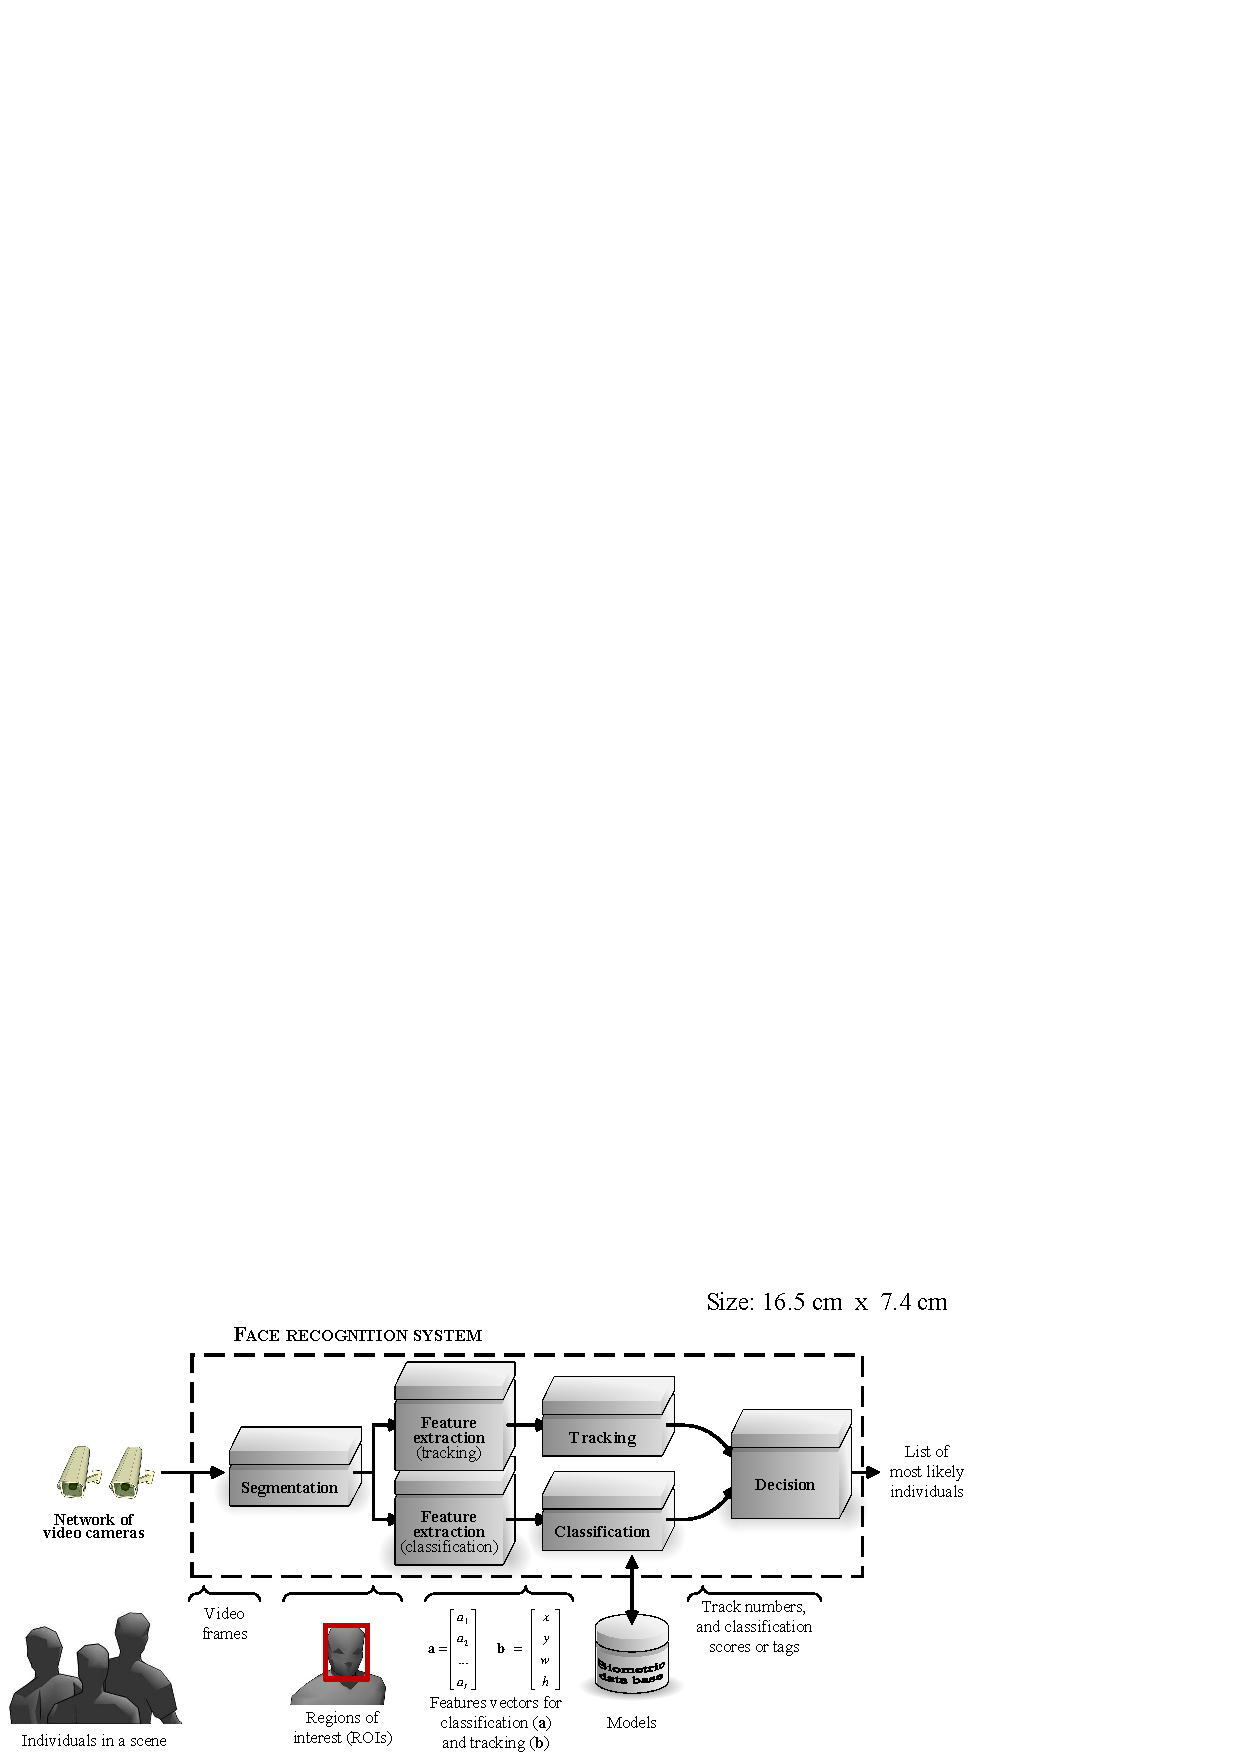
\includegraphics[width=0.97\linewidth, viewport= 0cm 0cm 16.5cm 7.4cm, clip]
 		              {c2_fig6}  }
	\caption{A generic track-and-classify biometric system for video-based face recognition}
	\label{fig:c2_faceRec}
\end{figure*}
%-------------------------- /Face recognition system --------------------------%

Several powerful techniques have been proposed to recognize faces in static 2D images (\cite{zhao03}).
A common approach to recognize faces in video consists in exploiting only spatial information (\emph{i.e.}, appearance), and applying extensions of static image-based techniques on high quality face images produced through segmentation.
The predominant techniques are appearance-based methods like Eigenfaces, and feature-based methods like Elastic Bunch Graph Matching (\cite{zhao03}).
More recently, some authors have exploited temporal information contained in video sequences to improve performance of video-based face recognition.
For example, track-and-classify systems (as the one shown in Figure \ref{fig:c2_faceRec}) combine spatial information with information on motion and appearance of faces in a scene (\cite{connolly10}).
Regardless, the performance of these techniques may degrade considerably when applied in real-world applications.

In addition to difficulties mentioned earlier, video-based face recognition remains a very challenging problem since faces captured in video frames are typically low quality and generally small.
Moreover, there are limitations associated with the camera and techniques used for segmentation, scaling, filtering, feature extraction, and classification (\emph{e.g.}, resolution and noise) (\cite{gorodnichy05, matta09, zhou03}).

%---------------------------- subsection : Database ---------------------------%
\subsection{Video data bases}
\label{sec:c2_db}

In this chapter, experiments are performed by applying AMCS to video-based face recognition in a closed-set access control (identification) applications.
Proof-of-concept simulations are performed with two real-world video data bases for face recognition.

The first data base was collected by the Institute for Information Technology of the Canadian National Research Council (IIT-NRC) (\cite{gorodnichy05}).
It is composed of 22 video sequences captured from eleven individuals positioned in front of a computer.
For each individual, two color video sequences of about fifteen seconds are captured at a rate of 20 frames per seconds with an Intel web cam of a $160\times120$ resolution that was mounted on a computer monitor.
Of the two video sequences, one is dedicated to training and the other to testing.
They are taken under approximately the same illumination conditions, the same setup, almost the same background, and each face occupies between $1/4$ to $1/8$ of the image.
This data base contains a variety of challenging operational conditions such as motion blur, out of focus factor, facial orientation, facial expression, occlusion, and low resolution.
The number of ROIs detected varies from class to class, ranging from 40 to 190 for one video sequences.

The second video data base is called Motion of Body (MoBo), and was collected at Carnegie Mellon University under the HumanID project (\cite{gross02}).
Each video sequence shows one of 25 different individuals on a tread-mill so that they move their heads naturally to four different motion types when walking: slowly, fast, on an inclined surface, and while carrying an object.
Six Sony DXC 9000 cameras, with a resolution of a $640\times480$ pixels, are positioned at different locations around the individuals.
Only the video sequences with visible faces were kept: full frontal view and both sides with an angle of about $70^\circ$ with the full frontal view.

In both cases, segmentation is performed using the Viola-Jones algorithm included in the OpenCV C/C++ computer vision library.
For the IIT-NRC database, the small regions of interest (ROIs) produced are converted in gray scale and normalized to $24\times24$ images where the eyes are aligned horizontally, with a distance of 12 pixels between them.
Principal Component Analysis is then performed to reduce the number of features.
The 64 features with the greatest eigenvalues are extracted and vectorized into $\textbf{a} = \{a_1, a_2, ..., a_{64}\}$, where each feature $a_i \in [0,1]$ are normalized using the min-max technique.
Learning is done with ROIs extracted from the first series of video sequences (1527 ROIs) while testing is done with ROIs extracted from the second series of video sequences (1585 ROIs).
The ROIs obtained with the MoBo data base where processed with Local Binary Pattern and Principal Component Analysis to produce 32 features vectors, also normalized using the min-max technique.
ROIs from sequences for each type of walk and view are divided in two; the first half is used for learning and the second half, for testing.
This yields a total of 36374 learning patterns and 36227 test patterns.
In both cases, the number of features was fixed after error convergence with a 1NN classifier trained on the learning data bases and tested on the test data base.

%------------------------------------------------------------------------------%
\subsection{Incremental learning scenarios}
\label{sec:c2_scenario}

Prior to computer simulations, each video data set is divided in blocks of data $D_t$, where $1\leq t\leq T$, to emulate the availability of $T$ successive blocks of training data to the AMCS during a biometric identification application.
Supervised incremental learning is performed according to two different scenarios.

\subsubsection{Enrollment}

In this scenario, each block contains ROIs of individuals that are not enrolled to the system.
Classes are added incrementally to the system, one at a time.
To assess AMCS performance for $K$ classes, the first learning block $D_1$ is composed of two classes, and each successive block $D_t$, where $2 \leq t \leq K-1$, contains the ROIs captured in a video sequence corresponding to an individual that has not previously been enrolled to the system.
For each $D_t$, performance is only evaluated for existing classes.
To insure the invariance of results to class presentation orders, this experiment is performed using five different random \emph{class} presentation orders.

\subsubsection{Update}

In this scenario, each block contains ROIs of individuals that have previously been enrolled to the system.
It is assumed that at a given time, the ROIs of an individual is captured in a video sequence, and then learned by the system to refine its internal models.
To assess AMCS performance, all classes are initially learned with the first data block $D_1$ and are updated one class at a time with blocks $D_2$ through $D_{K+1}$.
In order to better observe cases where classes are not initially well defined,
block $D_1$ is composed of $10\%$ of the data for each class, and each subsequent block $D_t$, where $2 \leq t \leq K+1$, is composed of the remaining $90\%$ of one specific class.
Here again, invariance to class order presentation is insured by repeating this experimentation with five different \emph{class} presentation orders.

%--------------------- SUBSECTION : Experimental protocol ---------------------%
\subsection{Experimental protocol}
\label{sec:c2_protocol}

To illustrate (1) the performance of Algorithm \ref{alg:c2_pso} with different ensemble selection methods and (2) the impact of diversity in the optimization environment on the models in the classification environment, the results of two experiments are presented in this chapter.
The performance of the proposed DPSO-based learning strategy is first evaluated and compared with various techniques to generate and select classifiers during supervised incremental learning of data blocks $D_t$.
Secondly, the correlation between particle diversity among particles in a swarm (in the hyperparameter) space and diversity among classifiers in an ensemble (in the feature and decision space) is shown empirically .

The DNPSO parameters used for both experiments are shown in Table \ref{tab:c2_pso}.
Weight values $\{w_1,w_2\}$ were defined as proposed in \cite{kennedy07}, and to detect a maximal number of local optima, no constraints were considered regarding the number of subswarms.
Since Euclidean distances between particles are measured with the DNPSO algorithm, the swarm evolves in a \emph{normalized} $\mathbb{R}^4$ space to avoid any bias due to the domain of each hyperparameter.
Before being applied to FAM, particle positions are denormalized to fit the hyperparameters domain.
For each new blocks of data $D_t$, the DPSO optimization process is set to either stop after 10 iterations without improving the classification rate of the best FAM network ($\textit{FAM}_{n^*,t}$) classification rate, or after maximum 100 iterations.

%------------------------------ DNPSO parameters ------------------------------%
\begin{table*}[t]
  \centering
  \caption{DNPSO parameters}
  \begin{tabular*}{\linewidth}{@{\extracolsep{\fill}}|lr|}
  	\hline
	  \textbf{Parameter} & \textbf{Value}     										\\ \hline
		Swarm's size $N$												&  40    						\\
		Weights $\{w_1,w_2\}$ 									&  $\{0.73,2.9\}$ 	\\
		Maximal number of subswarms   					&  $\infty$					\\
		Maximal size of each subswarm 					&  4								\\
		Neighborhood size												&  5    						\\
		Minimal distance between two masters    &  0.1   						\\
		Minimal velocity of free particles    &  0.0001    				\\ \hline
	\end{tabular*}
	\label{tab:c2_pso}
\end{table*}
%------------------------------ \DNPSO parameters -----------------------------%

Learning is performed over ten trials using ten-fold cross-validation with the LTM used as specified in (cite{connolly10}).
The proportion of $D_t$ assign to the LTM, and the maximal number of patterns for each class present in the LTM, are respectively set to $\lambda_D=1/6$ and $|LTM|_k=20$.
Out of the ten folds, eight are dedicated to training ($D_t^\text{t}$), one fold is combined with half of LTM to validate and determine the number of FAM training epochs ($D_t^\text{v}$), and the remaining fold is combined with the other half of the LTM to estimate the fitness of each particle during the DPSO algorithm ($D_t^\text{f}$).
Between successive training epochs, the presentation order of training patterns is changed randomly.
Within each trial, five different replications are performed using different class presentation order, for a total of 50 replications.

The simulations evaluate the performance achieved during both incremental learning scenarios of new data blocks $D_t$, where AMCSs employ the DPSO-based strategy proposed in Section \ref{sec:c2_algo} (Algorithms \ref{alg:c2_pso} and \ref{alg:c2_ens}) to evolve heterogeneous ensemble indicated by LBESTS$_\text{+d}$ (local best particles combined with the diversity greedy search).
This system is compared to AMCSs using the DPSO-based strategy but with different ensemble selection techniques, in particular:
\begin{itemize}
	\item GREEDY$_\text{a}$ $\leftarrow$ the ensemble of FAM networks found using greedy search based on accuracy (\cite{ulas09}),
	\item SWARM $\leftarrow$ the ensemble of FAM networks build with the entire swarm, and 
	\item GBEST $\leftarrow$ the FAM network corresponding to the DPSO global best solution.
\end{itemize}
For references, the performance is also given for an AMCS that uses the entire swarm of FAMs trained with a canonical PSO batch learning strategy (\cite{granger07}) (PSO$_\text{B}$), and a single \textit{k}NN classifier that also performs batch learning.
At a given time $t$, batch learning consist of initializing the system, and learning all the data blocks $D_t$ accumulated so far, $B_t = D_1\cup...\cup D_t$ (\cite{granger07}).

%-------------------------------- Experiment A --------------------------------%
\begin{figure*}[t]
  \centering
  \fbox{
	\subfloat[2D example]   {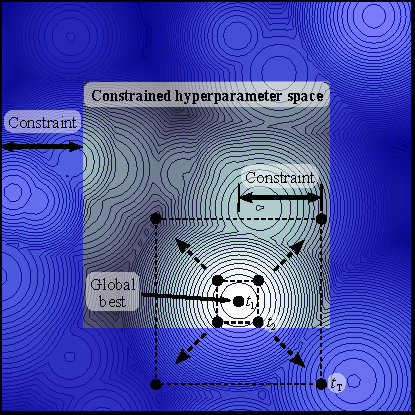
\includegraphics[width=0.44\linewidth]{c2_fig7a}
	         \label{fig:c2_proofEx} }
	\hspace*{10mm}
	\subfloat[2D projection]{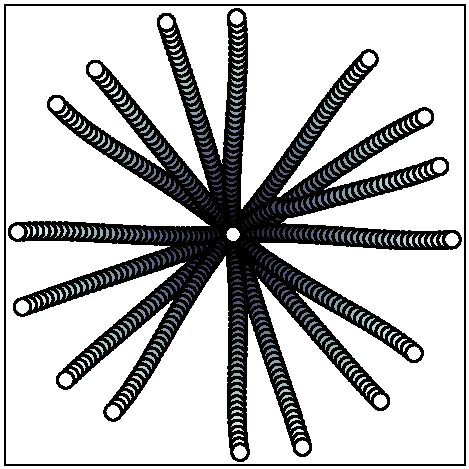
\includegraphics[width=0.44\textwidth]{c2_fig7b}
	         \label{fig:c2_proofPr}	}
	}
  \caption{Example of the particle positions for a 2D objective function (\ref{fig:c2_proofEx}) and 2D projection, obtained using Sammon's mapping of the particle positions in the $R^4$ hyperparameter space (\ref{fig:c2_proofPr}).
The swarm is organized into a hypercube centered around the global best in the in the normalized $R^4$ hyperparameter space.
The hypercube gradually expands, linearly changing particle diversity and affecting the corresponding ensemble of classifiers}
	\label{fig:c2_proof}
\end{figure*}
%------------------------------- \experiment A --------------------------------%

Additional experiments (presented in Figure \ref{fig:c2_proof}) verify the hypothesis under which particle diversity in the optimization environment is correlated to that of ensemble classifier diversity, where each classifier is associated to a particle.
Experiments are performed in two steps: (1) optimization during supervised batch learning of the whole IIT-NRC data base with the DPSO learning strategy, and (2) particles expansion.

Prior to optimization of hyperparameters, the normalized search space is bound by a constraint of 0.2.
Once the global best hyperparameter values are found, an ensemble is formed with 17 FAM networks, each one associated with a particle organized into a hypercube centered around the global best in the normalized $R^4$ hyperparameter space.
One particle is centered at the global best while the other 16 ($2^4$) are positioned as a 4 dimensions hypercube around the center. 
To change the diversity level, all particles are initially situated at the same position of the global best, and the size of the hypercube is gradually expanded up to the value of the constraint to form different swarms (each noted by a different color in Figure \ref{fig:c2_proofPr}).
The expansion of this hypercube will affect a change on diversity in the hyperparameter space.

%--------------------- subsection : performance indicator ---------------------%
\subsection{Performance evaluation and diversity indicator}
\label{sec:c2_indicator}

The average performance of AMCSs is assessed in terms of classification rate over a sequence of one or more ROIs, and resource requirements.
The \emph{classification rate for single facial images (ROIs)} is the ratio of correct predictions over all test set predictions, where each ROIs is tested independently.
Note that classification decisions produced for a single image are considered to be the most conservative performance metric, and it is used for fitness estimation in Algorithms \ref{alg:c2_pso} and \ref{alg:c2_ens}.
However, for the video-based face recognition application, \emph{classification
rate for video sequences} (over two or more ROIs), the result of the fusion between the tracking and classification module, is used.
Given video sequences, it is the ratio of correct predictions over all predictions made by the AMCS accumulated response over a fixed number of video frames.
For unbalanced data bases (\emph{i.e.}, video sequences of different length), classification rate for a number of frames exceeding the length of shorter sequences are computed with predictions obtained with all ROIs of the latter.
The accuracy of AMCSs is also evaluated with cumulative match curves (CMC) (\cite{moon01}).
These curves estimate the ranking capabilities of a classification system for identification applications by providing a cumulative a posteriori probability estimation of having a correct prediction according to rank.

Resource requirements of AMCSs that employ the DPSO learning strategy is measures in terms of \emph{compression}.
That is, the average number of training patterns, contained in all $D_t^\text{t}$ presented to the AMCS, per category prototype in the classifier.
For FAM networks, compression refers to the average number of training patterns per neuron in the $F_2$ layer.
For ensembles, it is the total number of $F_2$ layer nodes for all classifiers in the ensemble.
Since learning with \textit{k}NN consist of memorizing the training data set $D_t^\text{t}$, compression in this case is always one.

While particle swarm diversity is computed using Equation \ref{eq:c2_divPso}, three pairwise indicators are used to compute correlation, or diversity, between two ensemble's classifiers $e_1$ and $e_2$.
As with most measures present in literature, the $Q$ statistic and the correlation coefficient (\cite{ulas09}) rely on classifier disagreement to compute correlation among classifiers.
On the other hand, a specialized ambiguity indicator, inspired by margin theory (\cite{tang06}), is used to compute FAM network diversity.
For two ensemble classifiers $e_1$ and $e_2$, and a given data set (in our case the fitness estimation data set $D_t^\text{f}$), each pairwise indicator is computed as followed:
\begin{enumerate}
	\item \textbf{The $Q$ statistic:}
		\begin{equation} \label{eq:c2_Q}
	    Q_{e_1e_2} \in [0,1] =
	              \frac{N_{11}N_{00}-N_{10}N_{01}}{N_{11}N_{00}+N_{10}N_{01}},
		\end{equation}
where $N_{11}$, $N_{00}$, $N_{10}$, and $N_{01}$ are the number of patterns for each combination of correct and incorrect predictions by classifiers $e_1$ and $e_2$ on the given data set (see Table	\ref{tab:c2_Qstat}).
	\item \textbf{Correlation coefficient:}
\begin{equation}  \label{eq:c2_r}
	\begin{split}
		 \lefteqn{\rho_{e_1e_2} \in [0,1] =}\\
	   & \frac{ N_{11}N_{00} - N_{10}N_{01} }
		{\sqrt{(N_{11}+N_{10})(N_{01}+N_{00})(N_{11}+N_{01})(N_{10}+N_{00}) }},
	\end{split}
\end{equation}
%		\begin{equation}
%		  \rho_{e_1e_2} \in [0,1] = \frac{ N_{11}N_{00} - N_{10}N_{01} }
%		{\sqrt{(N_{11}+N_{10})(N_{01}+N_{00})(N_{11}+N_{01})(N_{10}+N_{00}) }},
%			\label{eq:c2_r}
%		\end{equation}
	\item \textbf{Specialized ambiguity indicator for FAM networks:} Given a pattern $\textbf{a}$, the FAM network selects the $F_2$ winning node $j^*$, corresponding to the highest choice function $T_{j}(\textbf{a})$, and predicts class $k(j^*)$. FAM ambiguity is defined by: 
		\begin{equation}
			\theta_e \in[0,1] = T_{j^*}(\textbf{a}) -
			                \texttt{max}(T_{j}(\textbf{a}), k\neq k^*).
		\end{equation}
Diversity between two FAM classifiers $e_1$ and $e_2$ is defined by the sum of the ambiguity differences for all patterns in the fitness estimation data set ($|D_t^\text{f}|$):
		\begin{equation}
			\Delta\theta_{e_1e_2} \in]0,|D_t^\text{f}|] =
	                   \displaystyle\sum^{|D_t^\text{f}|}
	                   |\theta_{e_1}-\theta_{e_2}|.
			\label{eq:c2_divFam}
		\end{equation}
\end{enumerate}

Ensemble diversity is then defined as the average value deprived from all combination of the pairwise classifier diversity indicators, computed in the same manner as Equation \ref{eq:c2_divPso}. 
Measures from Equations \ref{eq:c2_Q}, \ref{eq:c2_r}, and \ref{eq:c2_divFam} are noted: $\overline{Q_{e_1e_2}}$, $\overline{\Delta \rho_{e_1e_2}}$, and $\overline{\Delta \theta_{e_1e_2}}$.
Higher ensemble diversity is observed for low correlation indicators values ($\overline{Q_{e_1e_2}}$ and $\overline{\Delta \rho_{e_1e_2}}$) and for high values of the FAM diversity indicator ($\overline{\Delta \theta_{e_1e_2}}$).

%--------------------------------- Q statistic --------------------------------%
\begin{table}[t]
  \centering
  \caption{Contingency table used to compute diversity among ensemble classifiers with the $Q$ statistic and correlation coefficient}
  \begin{tabular}{|l|cc|}
  	\hline
  	& $\textit{FAM}_{e2}$ correct & $\textit{FAM}_{e2}$ incorrect \\ \hline
  	$\textit{FAM}_{e1}$ correct   & $N_{11}$ & $N_{10}$ \\ 
  	$\textit{FAM}_{e1}$ incorrect & $N_{01}$ & $N_{00}$ \\ \hline
	\end{tabular}
	\label{tab:c2_Qstat}
\end{table}
%-------------------------------- \Q statistic --------------------------------%

%------------------------------------------------------------------------------%
%------------------------------------------------------------------------------%
%---------------------------- Results & Discussion ----------------------------%
\section{Results and discussion}
\label{sec:c2_results_discussion}

%------------------------------------------------------------------------------%
\subsection{Performance for single images (ROIs)}

To assess the performance of ensembles evolved using the DPSO-based learning strategy, Figures \ref{fig:c2_add} and \ref{fig:c2_upd} present the average classification rate obtained with single facial regions of interest (ROIs), compression, and ensemble size achieved versus the number of data blocks $D_t$.
Results obtained after learning all IIT-NRC and MoBo data bases with both learning scenarios are shown in Tables \ref{tab:c2_add} and \ref{tab:c2_upd}.
For both incremental learning scenarios, results are shown for AMCSs that employs the DPSO-based strategy proposed in Section \ref{sec:c2_algo} (LBESTS$_\text{+d}$).
It is compared to ensembles formed with the entire swarm of FAM networks (SWARM) and the global best network only (GBEST).
In all cases, the accuracy-based greedy search (\cite{ulas09}) (GREEDY$_\text{a}$) is unable to improve the recognition capabilities of the single global best network (GBEST).
Its performances are thus not shown.  
For reference, performance is also shown for batch learning with an ensemble formed with the entire swarm (PSO$_\text{B}$) and the $k$ nearest neighbors algorithm (\textit{k}NN).
For face recognition on single ROIs from the IIT-NRC data base, \cite{arandjelovic09} was able to achieve a classification rate of 91\%, while \cite{gorodnichy05} obtained a classification of 80\%.
In both cases, batch learning was performed with settings in \cite{gorodnichy05}; that is, the features are vectorized as unprocessed gray scale values of the $24 \times 24$ images and one class was used to verify the false acceptance rate rather than the classification rate.
No such results are available for the MoBo data base.

%------------------------------------------------------------------------------%
%----------------------------- Enrollment scenario ----------------------------%

%-------------------------- Result - NRC & enrollment -------------------------%
\begin{figure*}[t]
  \centering
  \fbox{\begin{minipage}{0.97\linewidth}\centering
	\subfloat[]{ 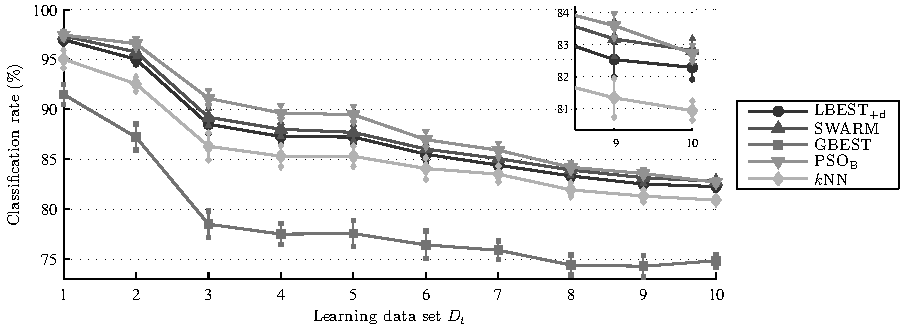
\includegraphics[width=0.95\linewidth]{c2_fig8a} 		 
							 \label{fig:c2_addErr} }  \\
	\subfloat[]{ 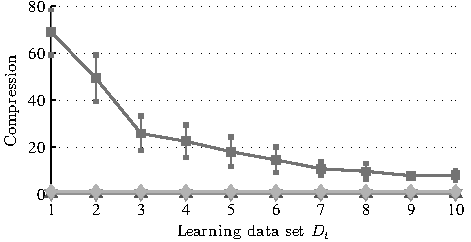
\includegraphics[width=0.47\linewidth]{c2_fig8b}
							 \label{fig:c2_addCpn} }	\quad
	\subfloat[]{ 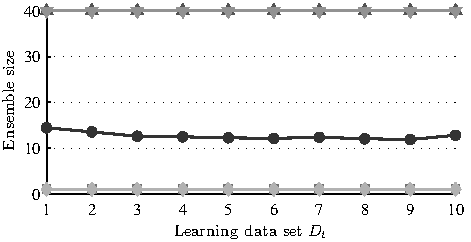
\includegraphics[width=0.47\linewidth]{c2_fig8c}
							 \label{fig:c2_addEns} }
  \end{minipage} }
	\caption{Average classification rate, compression, and ensemble size of the AMCS versus blocks of IIT-NRC data learned during the enrollment scenario.
Performance was evaluated during incremental learning for the AMCS with different ensemble selection techniques and the global best network alone (GBEST).
The performance of the whole swarm optimized during batch learning (PSO$_\text{B}$) and \textit{k}NN are shown for reference.
Error bars correspond to the 90\% confidence interval}
	\label{fig:c2_add}
\end{figure*}
%------------------------- \Result - NRC & enrollment -------------------------%

%---------------------------- Results - enrollment ----------------------------%
\begin{table*}[t]
 \small
 \centering
 \caption{Average classification rate (in percentage), compression and ensemble size after incremental learning of all the IIT-NRC and MoBo data bases for the enrollment scenario.
Each cell is presented with the 90\% confidence interval}
 \begin{tabular*}{\linewidth}{@{\extracolsep{\fill}}|l||rrr||rr|}
 	\hline
		Type of learning &\multicolumn{3}{c||}{Incremental} 
										 &\multicolumn{2}{c|}{Batch} \\ \hline
		Method &\textbf{LBESTS$_\text{+d}$} &SWARM &GBEST &PSO$_\text{B}$ &\textit{k}NN
		\\ \hline
		\multicolumn{6}{|l|}{\vspace{-5pt}}\\
		\multicolumn{6}{|l|}{\hspace{-5pt}\textbf{IIT-NRC data base}}	\\\hline
		Classification rate (\%) & $82.3\pm0.4$     & $82.8\pm0.4$
						 & $74.9\pm0.6$  & $82.7\pm0.2$     & $80.9\pm0.3$  \\
		Compression              & $0.38\pm0.03$    & $0.13\pm0.01$  
						 & $8\pm2$       & $0.062\pm0.003$  & $1\pm0$  			\\
		Ensemble size            & $12.8\pm0.6$     & $40\pm0$
						 & $1\pm0$			 & $40\pm0$         & $1\pm0$  			\\\hline
		\multicolumn{6}{|l|}{\vspace{-5pt}}\\
		\multicolumn{6}{|l|}{\hspace{-5pt}\textbf{MoBo data base}}		\\\hline
		Classification rate (\%) &$92\pm2$       &$91\pm5$
						  &$89.2\pm0.7$  &$94.9\pm0.1$   &$94.5\pm0.1$ 			\\
		Compression              &$1.3\pm0.1$    &$0.48\pm0.02$ 			
						  &$9.0\pm0.9$   &$0.09\pm0.02$  &$1\pm0$  					\\
		Ensemble size   				 &$12.1\pm0.4$   &$40\pm0$
						  &$1\pm0$       &$40\pm0$       &$1\pm0$  					\\\hline
	\end{tabular*}
	\label{tab:c2_add}
\end{table*}
%--------------------------- /Results - enrollment ----------------------------%

For the enrollment scenario, only two classes are present at the beginning of the learning process.
Class decision boundaries are initially simple and classification rates are high.
As classes are added, these boundaries become more complex, leading to a decline in classification rate (see Figure \ref{fig:c2_add}).
When the AMCS is used with the global best only (GBEST), compression also diminishes considerably.
While this is also true when the AMCS uses batch learning (PSO$_\text{B}$), compression and ensemble size for the AMCS with both ensembles methods remains stable during incremental learning.

As expected, after training on all data, GBEST gives the lowest classification rate, while all other solutions give classification rates between 81\% and 83\% (see Figure \ref{fig:c2_add} and Table \ref{tab:c2_add}).
Using LBESTS$_\text{+d}$ gives classification rate comparable to that of SWARM throughout all the enrollment process, except after learning new blocks at times $t=2$ and $t=10$.
However, as compression and ensemble size show (in Table \ref{tab:c2_add}), LBESTS$_\text{+d}$ is able to achieve this accuracy with a third of the resources.

Results with the MoBo data base are consistent with those obtained with the IIT-NRC data (see Table \ref{tab:c2_add}).
However, since position of individuals and video cameras used in the MoBo protocol are fixed, data acquisition is more constrained than with the IIT-NRC data base.
Class distributions are more compact and less likely to vary significantly from one block to the next.
Classification rate and compression follow similar trends excepted that they are generally higher than with the IIT-NRC data base.

%------------------------------------------------------------------------------%
%------------------------------- Update scenario ------------------------------%
%------------------------------------------------------------------------------%
The overall phenomena observed during enrollment resemble the performance observed for the update scenario.
The main difference is that all class distributions are defined from the outset, in $D_1$, and the AMCS initially has knowledge of the entire classification problem.
Due to limited learning data, knowledge of the problem is however incomplete and decision boundaries in the input feature space are then poorly defined, leading to a low classification rate (see Figure \ref{fig:c2_upd}).
As classes are updated incrementally, accuracy of the face recognition system tends to increase.
The highest classification rate are again obtained with LBESTS$_\text{+d}$ and SWARM (Table \ref{tab:c2_upd}).
Although the AMCS with LBESTS$_\text{+d}$ uses about one third of resources used by SWARM, both selection techniques have comparable accuracy over all data blocks, except at times $t=\left\{10,12\right\}$.

%---------------------------- Result - NRC & update ---------------------------%
\begin{figure*}[t]
  \centering
  \fbox{\begin{minipage}{0.97\linewidth}\centering
	\subfloat[]{ 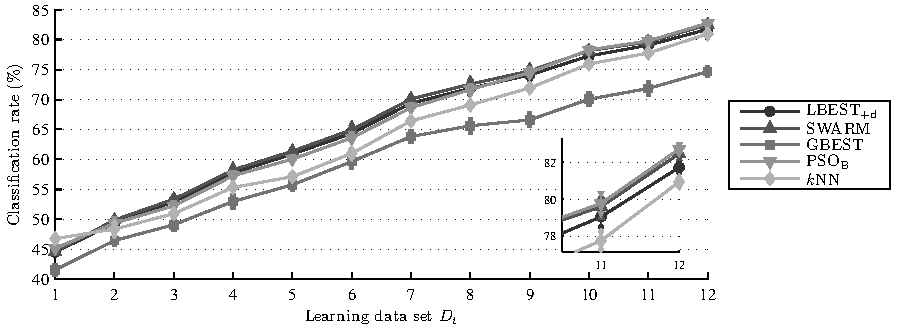
\includegraphics[width=0.95\linewidth]{c2_fig9a}
               \label{fig:c2_updErr} }	\\
	\subfloat[]{ 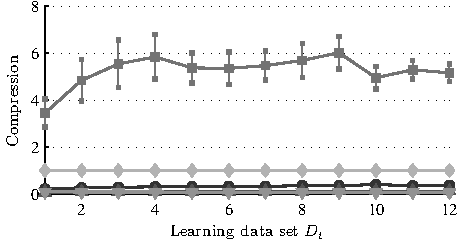
\includegraphics[width=0.47\linewidth]{c2_fig9b}
               \label{fig:c2_updCpn} } \quad
	\subfloat[]{ 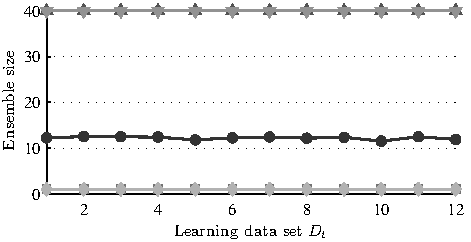
\includegraphics[width=0.47\linewidth]{c2_fig9c}
               \label{fig:c2_updEns} }
  \end{minipage} }
	\caption{Average classification rate, compression, and ensemble size of the AMCS versus blocks of IIT-NRC data learned during the update scenario.
Performance was evaluated during incremental learning for the AMCS with different ensemble selection techniques and the global best network alone (GBEST).
The performance of the whole swarm optimized during batch learning (PSO$_\text{B}$) and \textit{k}NN are shown for reference.
Error bars correspond to the 90\% confidence interval}
	\label{fig:c2_upd}
\end{figure*}
%--------------------------- \Result - NRC & update ---------------------------%

%------------------------------ Results - update ------------------------------%
\begin{table*}[t]
 \small
 \centering
 \caption{Average classification rate (in percentage), compression and ensemble size after incremental learning of all the IIT-NRC and MoBo data bases for the update scenario.
Each cell is presented with the 90\% confidence interval}
 \begin{tabular*}{\linewidth}{@{\extracolsep{\fill}}|l||rrr||rr|}
 	\hline
		Type of learning &\multicolumn{3}{c||}{Incremental} 
										 &\multicolumn{2}{c|}{Batch} \\ \hline
		Method &\textbf{LBESTS$_\text{+d}$} &SWARM &GBEST &PSO$_\text{B}$ &\textit{k}NN
		\\ \hline
		\multicolumn{6}{|l|}{\vspace{-5pt}}\\
		\multicolumn{6}{|l|}{\hspace{-5pt}\textbf{IIT-NRC data base}}	\\\hline
		Classification rate (\%) & $81.7\pm0.3$    & $82.5\pm0.3$ 
							& $74.7\pm0.7$ & $82.7\pm0.3$    & $80.9\pm0.3$ 	\\
		Compression              & $0.36\pm0.02$   & $0.11\pm0.01$
		          & $5.1\pm0.4$  & $0.062\pm0.003$ & $1\pm0$ 				\\
		Ensemble size						 & $11.9\pm0.5$    & $40\pm0$
							& $1\pm0$      & $40\pm0$        & $1\pm0$ 				\\\hline
		\multicolumn{6}{|l|}{\vspace{-5pt}}\\
		\multicolumn{6}{|l|}{\hspace{-5pt}\textbf{MoBo data base}}		\\\hline
		Classification rate (\%)  &$92.8\pm0.3$   &$95\pm3$     
		               &$87\pm2$  &$94.9\pm0.1$   &$94.5\pm0.1$ 		\\
		Compression               &$1.1\pm0.1$    &$0.37\pm0.02$ 
								   &$12\pm2$  &$0.09\pm0.01$  &$1\pm0$   				\\
		Ensemble size             &$13.0\pm0.8$   &$40\pm0$
									 &$1\pm0$   &$40\pm0$       &$1\pm0$   				\\\hline
	\end{tabular*}
	\label{tab:c2_upd}
\end{table*}
%----------------------------- /Results - update ------------------------------%

Two differences are observed at the beginning of the learning process with batch learning methods.
When using the AMCS with batch learning, the LTM is unnecessary, and all the cumulative data from successive blocks is directly assigned to the training, validation, and fitness estimation ($D_t^\text{t}$, $D_t^\text{v}$, and $D_t^\text{f}$).
Therefore, fewer data samples are used for validation during network training and fitness estimation on the objective function, leading to a lower classification rate than those obtained with the LTM.
Secondly, in contrast with FAM, where the Webber Law choice function computes city block distances ($L^1$ norm), \textit{k}NN instead computes Euclidean distances ($L^2$ norm).
It only relies on validation data only to set the value of $k$, and does not perform sequential learning (\emph{i.e.}, it is not sensitive to patterns order presentation).
As such, it performs well if only few samples are available to define decision boundaries in a complex classification environment where all classes are defined.
However, it must store all cumulative training data in memory, and requires a greater time complexity for matching input patterns to an output class.
Indeed, to perform predictions, FAM networks complement code the $I$ features, computes the choice function for the $J$ category prototypes in the ensemble, and find the best for each FAM, a time complexity of $O(2IJ)$.
On the other hand, \textit{k}NN computes the Euclidean distance for each $J$ category and ranks the solutions to find the best $k$, a time complexity of $O(kI J\text{log}(J))$.
For equal compression values, matching an input pattern to a class is thus a simpler task with a FAM classifiers, and the difference between the two increases over time, has more category prototype are include in the AMCS.

Results with the IIT-NRC data are once again confirmed by those obtained with the MoBo data (see Table \ref{tab:c2_upd}).
As with the enrollment scenario, class distributions are more compact and both classification rate and compression are higher.
However, updating classes through batch learning yields a higher classification rate at the expense of lower compression.

With DNPSO parameters presented in Table \ref{tab:c2_pso}, the AMCS was able to find on average $6.4\pm0.1$ local maxima (with the 90\% confidence interval) during the enrollment scenario, and $6.3\pm0.1$ for the update scenario.
Using the greedy search to select classifiers that maximize particle diversity (LBESTS$_\text{+d}$) nearly doubles the average number of classifiers used in the ensembles to $12.7\pm0.2$ and $12.2\pm0.1$ FAM networks, respectively (see Figures \ref{fig:c2_addEns} and \ref{fig:c2_updEns}).
These ensembles yield a classification rate comparable to that of the AMCS with SWARM, and are efficiently obtained by maximizing particle diversity in the hyperparameter space.
For instance, if the greedy search process where driven by classifier diversity in the classification environment, this would involve the costly computation of the Weber function (Equation \ref{eq:choice}) of every nodes of all FAM networks over each $D_t^\text{f}$ pattern every time a network is added to the ensemble by Algorithm \ref{alg:c2_ens}.

Note that, to initially find more local optima, the ratio $|$swarm$|$/$|$neighborhood$|$ could be raise.
But whereas large swarms would lead to a large number of fitness evaluation, unnecessarily slowing the DPSO optimization process, small neighborhoods sizes leads local optima detection that is very sensitive to noise on the objective function. 
The choice of those (DNPSO) parameters is problem dependent.

%------------------------------------------------------------------------------%
\subsection{Performance for video-streams (multiple ROIs)}

For video-based face recognition, classification is typically performed by accumulating the response of a classifier over several video frames.
For both scenarios, Figure \ref{fig:c2_vid} presents the evolution of the classification rate for video sequences achieved by the proposed system (LBESTS$_\text{+d}$) as a function of the number of ROIs used to perform identification, and Figure \ref{fig:c2_cmc} shows the cumulative match curves (CMC) for different number of ROIs used to perform identification.
Table \ref{tab:c2_vid} presents the number of ROIs necessary to achieve an average classification rate statistically comparable to $100\%$, for all tested cases and both data bases.
Comparison with other video-based face recognition systems from the literature is presented in Table \ref{tab:c2_vsOthers} for both IIT-NRC and MoBo data bases.

%---------------- Classification for video sequences - IIT-NRC ----------------%
\begin{figure*}[t]
  \centering
  \fbox{
	\subfloat[Enrollment scenario]{
		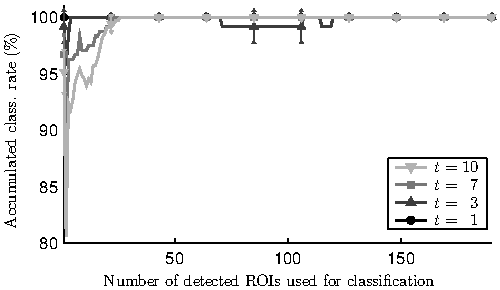
\includegraphics[width=0.46\linewidth]{c2_fig10a} 	
		\label{fig:c2_addVid} }
	\hspace*{4mm}
	\subfloat[Update scenario]{
		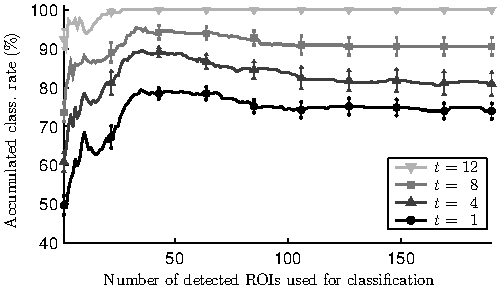
\includegraphics[width=0.46\linewidth]{c2_fig10b} 	
		\label{fig:c2_updVid} }
  }
	\caption{Evolution of the average classification rate for video sequences of the AMCS's ensemble versus the number of ROIs used to identify individuals of the IIT-NRC data base.
Performance is shown for incremental learning under both scenarios for the AMCS with LBESTS$_\text{+d}$.
Error bars correspond to the 90\% confidence interval}
	\label{fig:c2_vid}
\end{figure*}
%--------------- \Classification for video sequences - IIT-NRC ----------------%

As Figure \ref{fig:c2_vid} shows, the video-based classification rate for both scenarios follow the same trends as when the system is tested with single ROIs (Figures \ref{fig:c2_add} and \ref{fig:c2_upd}).
When classes are enrolled incrementally (Figure \ref{fig:c2_addVid}), class decision boundaries becomes more complex in time.
Accuracy obtained with few ROIs then decreases, while the number of ROIs necessary to achieve a video-based classification rate comparable to 100\% increases.
On the other hand, the video-based classification rate obtained after updating classes through incremental learning grows over time, as new blocks of data become available.
When blocks are available, the AMCS needs fewer ROIs to achieve a higher video-based accuracy and it is eventually comparable to 100\% with the same number of ROIs as during enrollment.

The effect on AMCS accuracy of video sequence length used to recognize individuals is also shown in Figure \ref{fig:c2_cmc}.
With each passing ROI, evidence in the form of class predictions is accumulated.
As FAM networks outputs are binary vector, the number of ROIs that predicts a class is instead accumulated and used to establish a ranking through majority voting.
The cumulative match curves in Figure \ref{fig:c2_cmc} show that as the length of the video sequences (and number of ROIs) increases, ambiguity regarding the predictions diminishes.
The probability of the correct class being the first ranked prediction increases to eventually reach 100\%, while the minimal ranking with a cumulative probability of 100\% also decreases to eventually reach 1.

%---------------------------- CMC curves - IIT-NRC ----------------------------%
\begin{figure*}[t]
  \centering
  \fbox{
	\subfloat[Enrollment scenario]{
		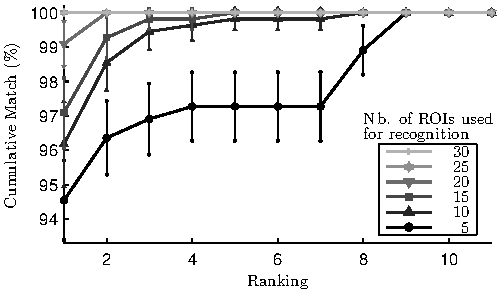
\includegraphics[width=0.46\linewidth]{c2_fig11a} 	
		\label{fig:c2_addcmc} }
	\hspace*{4mm}
	\subfloat[Update scenario]{
		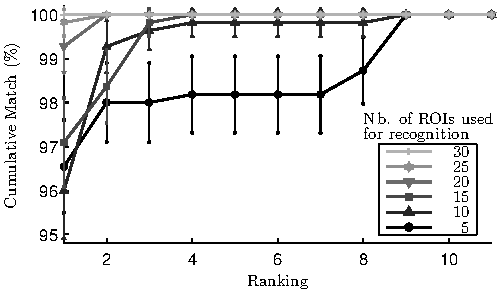
\includegraphics[width=0.46\linewidth]{c2_fig11b} 	
		\label{fig:c2_updcmc} }
  }
	\caption{Cumulative Match Curves the AMCS's ensemble for different number of ROIs used to perform face recognition.
Performance is shown after incremental learning of all the IIT-NRC data base, under both scenarios for the AMCS with LBESTS$_\text{+d}$.
Error bars correspond to the 90\% confidence interval}
	\label{fig:c2_cmc}
\end{figure*}
%--------------------------- \CMC curves - IIT-NRC ----------------------------%

When both learning and test sequences of the IIT-NRC data base were recorded, the individuals were all initially facing the camera, giving a full frontal image of their face.
The ROIs of the first frames are similar leading to classification rates obtained with the first pattern of each video sequences that are always higher than those obtained with a single ROI.
As the individuals begin moving, changing his facial orientation and expression, different facial views, corresponding to data points in new regions of the feature space, are presented to the system.
Since the first frames of each video sequence are initially present in $D_1$, the biometric face models are not well defined and these new regions in the feature space are then unexplored by the FAM networks.
Recognizing an individual toward the end of a video sequence is thus more difficult.
As the number of frames used to perform recognition increases, correct predictions for each ROIs accumulated at the beginning of the test sequences are surpassed by the wrong predictions accumulated with the subsequent ROIs.
Until all classes are updated, this leads to a video-based classification rate that tends to decrease at the end of each sequence. 

%------------------ Number of ROIs necessary to achieve 100% -----------------%
\begin{table*}[t]
	\small
	\centering
	\caption{Number of ROIs necessary to achieve a classification rate comparable to 100\% for video-based face recognition after learning the entire IIT-NRC and MoBo data bases through both incremental learning scenarios with the AMCS}
	\begin{tabular*}{\linewidth}{@{\extracolsep{\fill}}|l||rrr||rr|}
		\hline
		Type of learning &\multicolumn{3}{c||}{Incremental} 
										 &\multicolumn{2}{c|}{Batch} \\ \hline
		Method &\textbf{LBESTS$_\text{+d}$} &SWARM &GBEST &PSO$_\text{B}$ &\textit{k}NN
		\\ \hline
		
		\multicolumn{6}{|l|}{\vspace{-5pt}}\\
		\multicolumn{6}{|l|}{\hspace{-5pt}\textbf{IIT-NRC data base}}			\\\hline
		Number of ROIs during enrollment &24 &23 &never &19 &24 				\\
		Number of ROIs during update     &25 &20 &never &19 &24 				\\\hline
		
		\multicolumn{6}{|l|}{\vspace{-5pt}}\\
		\multicolumn{6}{|l|}{\hspace{-5pt}\textbf{MoBo data base}}				\\\hline
		Number of ROIs during enrollment &15 &30 &16 &32 &16 						\\ 
		Number of ROIs during update     &27 &25 &16 &32 &16 						\\\hline
	\end{tabular*}
	\label{tab:c2_vid}
\end{table*}
%----------------- \Number of ROIs necessary to achieve 100% -----------------%

In the worst case (the update scenario), Table \ref{tab:c2_vid} shows that the AMCS with the DPSO-based strategy needs 5 additional ROIs than with SWARM to have an accuracy comparable to 100\%.
Assuming ideal tracking performances and a camera that acquires video sequences at a rate of 30 frames per second, this represents around a fifth of a second.
This level of performance is also achieved with only a third of the resources (see Table \ref{tab:c2_add} and \ref{tab:c2_upd}). 
The number of additional ROIs needed to achieve a classification rate comparable to 100\% grows to six with ensembles obtained through batch learning of all cumulative data.
Results are similar with the MoBo data base, except for AMCSs with the proposed DPSO-based strategy which require fewer ROIs to achieved a 100\% classification rate.
The more controlled data acquisition conditions for MoBo also make it possible for a single FAM network to achieve a perfect video-based classification rate.

%------------------ Comparison with others - MoBo and IIT-NRC -----------------%
\begin{table*}[t]
% 	\footnotesize
	\small
	\centering
	\caption{Comparison of the DPSO-based learning strategy with other authors on the IIT-NRC and MoBo data bases.
Classification rates where obtained for recognition on video sequences}
	\begin{tabular*}{\linewidth}{@{\extracolsep{\fill}}|l|lllll|}
		\hline
		\multicolumn{6}{|l|}{\vspace{-5pt}}\\
		\multicolumn{6}{|l|}{\textbf{IIT-NRC data base}}
		\\ \hline
		Proposed syst. & Arandjelovic et al. & Gorodnichy &
		Tangelder et al. & Wang et al. & \\
		& (2009) & (2005) & (2006) & (2009) & \\
		100\%  & 100\%  & $95\%$  & $95\%$  & $93\%$ & \\\hline
		
		\multicolumn{6}{|l|}{\vspace{-5pt}}\\
		\multicolumn{6}{|l|}{\hspace{-5pt}\textbf{MoBo data base}}				\\\hline
		Proposed syst. & Cevikalp et al. & Hadid et al. &  Liu et al. &
		Wang et al. & Zhou et al. \\
		& (2010) & (2004) & (2003) & (2008) & (2003) \\
		$100\%$  & $98\%$ & $94\%$  & $99\%$  & $94\%$  & $100\%$
		\\ \hline
	\end{tabular*}
	\label{tab:c2_vsOthers}
\end{table*}
%----------------- \Comparison with others - MoBo and IIT-NRC -----------------%

Compared to other methods proposed in literature for video-based face recognition, an AMCS with the proposed DPSO learning strategy outperforms other systems, except that of \cite{arandjelovic09} with the IIT-NRC data base and \cite{zhou03} with the MoBo data base.
Regardless of the scenario, the AMCS with LBESTS$_\text{+d}$ must accumulate about 1 second of video stream to accumulate the ensemble responses and achieve a classification rates of 100\% after incremental learning of the entire MoBo data base.
In comparison, after performing \emph{batch learning} of the MoBo data base
\cite{zhou03} achieved the same result by accumulating classifier responses for 0.5 second.
While \cite{arandjelovic09} also obtained a 100\% video-based classification rate, the number of accumulated response to achieve this is not available.

%------------------------------------------------------------------------------%
%------------------------------------------------------------------------------%
\subsection{Particle diversity -vs- classifier diversity}
\label{sec:c2_expDiv}

%---------------------------------- Diversity ---------------------------------%
\begin{figure*}[t]
  \centering
  \fbox{
	\subfloat[]{
	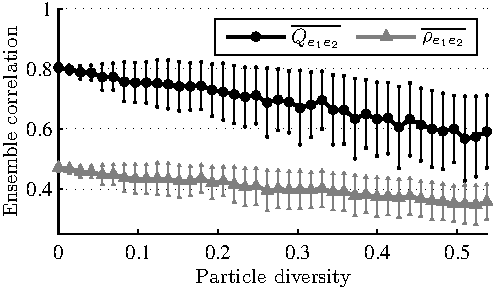
\includegraphics[width=0.46\linewidth]{c2_fig12a} \label{fig:c2_corr} }
	\hspace*{1mm}
	\subfloat[]{
	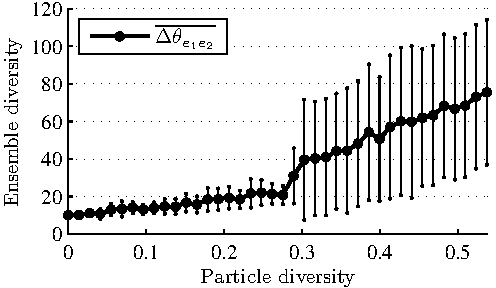
\includegraphics[width=0.46\linewidth]{c2_fig12b} \label{fig:c2_amb} }
  }
  \caption{Ensemble diversity in the classification environment as a function of particle diversity ($\overline{\delta_{e_1e_2}}$) in the optimization environment.
Ensemble diversity is shown using two correlation indicators ($\overline{Q_{e_1e_2}}$ and $\overline{\rho_{e_1e_2}}$ in Figure \ref{fig:c2_corr}), and an diversity indicator ($\overline{\Delta\theta_{e_1e_2}}$ in Figure \ref{fig:c2_amb}).
A decrease in correlation signifies an increase in diversity.
Each indicator is shown with its 90\% confidence interval}
  \label{fig:c2_diversity}
\end{figure*}
%--------------------------------- \Diversity ---------------------------------%

As mentioned, the DPSO-based incremental learning strategy is based on the hypothesis that particle diversity in the hyperparameter space implicitly generates diversity in the feature space, among classifiers associated with those particles.
Based on the experiment introduced in Figure \ref{fig:c2_proof}, this hypothesis is verified.
Figures \ref{fig:c2_diversity} presents the value of three classifiers correlation/diversity indicators -- $Q$ statistic (Equations \ref{eq:c2_Q}), Correlation coefficient (Equation \ref{eq:c2_r}), and the specialized ambiguity indicator for FAM networks (Equation \ref{eq:c2_divFam}) -- as a function of particle diversity in the hyperparameter space (Equation \ref{eq:c2_divPso}) when training on the IIT-NRC data base.
Figures \ref{fig:c2_addDiv} and \ref{fig:c2_updDiv} also show the classifier and particle diversity obtained during incremental learning for AMCS where ensembles are formed with LBESTS$_\text{+d}$ and SWARM.

FAM performs sequential learning of training patterns.
Therefore, decision boundaries created during training depends heavily on patterns presentation order.
Given that this order is typically determined randomly, prior each training epoch, an ensemble's classifiers will differ, even though they were trained with the same hyperparameters (see Figure \ref{fig:c2_diversity}).
When all particles are initially positioned at the global best position, this yields correlation indicators that are lower than one ($\overline{Q_{e_1e_2}}=0.80\pm0.01$ and $\overline{\rho_{e_1e_2}}=0.47\pm0.01$) and a diversity indicator higher than 0 ($\overline{\Delta\theta_{e_1e_2}}=0.07\pm0.01$).

As the hypercube expands (see Figure \ref{fig:c2_proof}), particle swarm diversity increases linearly.
No matter if diversity is computed in the decision space with the correlation indicators based on ensemble disagreement ($\overline{Q_{e_1e_2}}$ and $\overline{\rho_{e_1e_2}}$), or with ambiguity in the feature space ($\overline{\Delta\theta_{e_1e_2}}$), classifier diversity (correlation) follows the same trend by increasing (decreasing) constantly.
Depending on the indicator, diversity in the classification environment changes significantly for different levels of particle diversity: the $Q$ statistic differs for $\overline{\delta_{e_1e_2}}=0.26$ ($\overline{Q_{e_1e_2}}=0.7\pm0.1$), correlation differs for $\overline{\delta_{e_1e_2}}=0.25$ ($\overline{\rho_{e_1e_2}}=0.41\pm0.06$), and ambiguity-based diversity differs for $\overline{\delta_{e_1e_2}}=0.09$ ($\overline{\Delta\tau_{e_1e_2}}=0.10\pm0.02$).
Overall, results confirm the initial hypothesis that diversity in the hyperparameter space does indeed translates to diversity among classifiers in the feature space.

It is important to note that FAM networks are very sensitive to the match tracking hyperparameter ($\epsilon$) when it is close to zero.
Indeed, positive and negative values of $\epsilon$ have opposite effect on the dept of search performed among $F_2$ nodes when training on a pattern $\textbf{a}$.
When a winning $F_2$ node $j^*$ leads to a prediction error, positive (negative) values of $\epsilon$ restricts (relaxes) the condition on which subsequent $F_2$ nodes passes the vigilance test.
With $\epsilon>0$ ($\epsilon<0$), FAM tends to create more (fewer), but smaller (larger), category hyper-rectangles, leading to narrow (broad) generalization.
This explains the large confidence interval observed when $\overline{\delta_{e_1e_2}} > 0.3$.
For two out of ten replications, the global best position found during DPSO optimization leads to global optimal values with $\epsilon \in [-0.03, 0.06]$. 
When particle diversity reaches $\delta=0.3$, ensembles are then formed of classifiers with both positive and negative match tracking values, leading to a considerable classifier diversity ($\overline{\Delta\theta_{e_1e_2}} > 200$).

%------------------- Particles - Diversity during enrollment ------------------%
\begin{figure*}[t]
  \centering
  \fbox{\begin{minipage}{0.97\linewidth}\centering
	%-- Diversity
	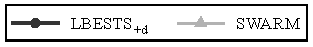
\includegraphics[width=0.4\linewidth]{c2_fig13-14_leg} \\
	\subfloat[Particle diversity]{
		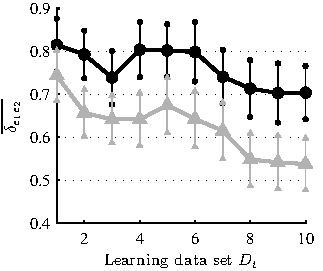
\includegraphics[width=0.31\linewidth]{c2_fig13a} 
		\label{fig:c2_addDivSwm} }
	\hspace*{1.5mm}
	\subfloat[Classifier diversity]{
		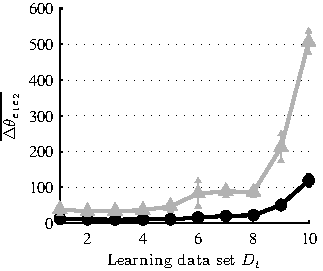
\includegraphics[width=0.31\linewidth]{c2_fig13b} 	
		\label{fig:c2_addDivFam} }
	\hspace*{1.5mm}
	\subfloat[Scatter plot]{
		\includegraphics[width=0.31\linewidth]{c2_fig13c} 	
		\label{fig:c2_addDivCor} }
  \end{minipage} }
	\caption{Particle and classifier diversity of the AMCS's ensembles versus the number of learning blocks during the enrollment learning scenario (Figures \ref{fig:c2_addDivSwm} and \ref{fig:c2_addDivFam}).
The FAM ambiguity indicator (Equation \ref{eq:c2_divFam}) was used for classifier diversity and all results are presented with their 90\% confidence interval.
Also shown is classifier diversity as a function of the particle diversity using all data points (Figure \ref{fig:c2_addDivCor})}
	\label{fig:c2_addDiv}
\end{figure*}
%------------------ /Particles - Diversity during enrollment ------------------%

%--------------------- Particles - diversity during update --------------------%
\begin{figure*}[t]
  \centering
  \fbox{\begin{minipage}{0.97\linewidth}\centering
	%-- Diversity
	\includegraphics[width=0.4\linewidth]{c2_fig13-14_leg} \\
	\subfloat[Particle diversity]{
		\includegraphics[width=0.31\linewidth]{c2_fig14a} 	
		\label{fig:c2_updDivSwm} }
	\hspace*{1.5mm}
	\subfloat[Classifier diversity]{
		\includegraphics[width=0.31\linewidth]{c2_fig14b} 	
		\label{fig:c2_updDivFam} }
	\hspace*{1.5mm}
	\subfloat[Scatter plot]{
		\includegraphics[width=0.31\linewidth]{c2_fig14c} 	
		\label{fig:c2_updDivCor} }
  \end{minipage} }
	\caption{Particle and classifier diversity of the AMCS's ensemble versus the number of learning block during the update learning scenario (Figures \ref{fig:c2_updDivSwm} and \ref{fig:c2_updDivFam}).
The ambiguity indicator (Equation \ref{eq:c2_divFam}) was used for classifier diversity and all results are presented with their 90\% confidence interval.
Also shown is the classifier diversity as a function of the particle diversity using all data points (Figure \ref{fig:c2_updDivCor})}
	\label{fig:c2_updDiv}
\end{figure*}
%-------------------- /Particles - diversity during update --------------------%

However, as results shown in Figures \ref{fig:c2_addDiv} and \ref{fig:c2_updDiv}, the relation between particle and classifier diversity during incremental learning is not as simple as with batch learning.
When data is learned incrementally over time, FAM decisions boundaries may be adjusted to accommodate new classes.
In the hyperparameter space, the objective function changes over time and regions with potential optima become increasingly localized (\cite{connolly10}).
Diversity in the hyperparameter space then decreases gradually, and convergence of subswarms toward local optima reduces particle swarm diversity below that obtained with the greedy search process. 
Under the update scenario, all classes are represented at the beginning of the learning process, and FAM networks are more complex, which increases the impact of the hyperparameters used during training.
Even if particle diversity values for $D_1$ are lower than those obtained during enrollment, classifier diversity is typically about ten times higher.
This increased complexity leads to an increased variation across the different replications, resulting in larger confidence intervals for particle diversity.
Even if results are comparable for AMCSs with LBESTS$_\text{+d}$ and SWARM (Figure \ref{fig:c2_updDivSwm}), LBESTS$_\text{+d}$ still tends to provide the highest particle diversity.

Meanwhile, in the feature space, FAM networks are trained using different hyperparameters and different pattern presentation orders with each passing $D_t$.
As shown in Figure \ref{fig:c2_addDiv}, as new data is learned by the AMCS, the ensemble of classifiers becomes increasingly diverse.
Figures \ref{fig:c2_addDivCor} and \ref{fig:c2_updDivCor} illustrate that, in a context of incremental learning, there is an inverse relationship between particle and classifier diversity.
As mentioned, the higher ensemble diversity observed with SWARM does not translate to a significantly higher classification rate for the ensemble.

Note that this does not contradict results presented in Figure \ref{fig:c2_diversity}, where a diversity analysis is performed with FAM networks that are initially all in the same state prior learning the whole IIT-NRC data base with batch learning.
Instead, for each learning data set $D_t$, Figures \ref{fig:c2_addDiv} and \ref{fig:c2_updDiv} present only one point in the particle--classifier diversity space of what is a diversity analysis when using the greedy search process (Algorithm \ref{alg:c2_ens}) on a local time frame and with networks that are in different initial conditions.

%--------------------------------- Conclusion ---------------------------------%
\section{Conclusion} \label{sec:c2_conclusion}

%-- Paper objective
In this chapter, an incremental learning strategy based on DPSO is proposed to evolve heterogeneous ensembles of classifiers in response to new data.
This strategy is applied to an AMCS for video-based face recognition consisting of a pool of FAM neural networks to classify face regions, the DNPSO algorithm to optimize classifier parameters such that classification rate is maximized.
The dynamic swarm properties are then exploited to perform an ensemble selection process based on accuracy and diversity.

Overall results confirm that there is indeed a correlation between diversity in the optimization environment and diversity in the classification environment.
The diversity of solutions can easily be controlled in the optimization environment with a DPSO algorithm, and allows for an efficient selection of diversified ensembles of classifiers.
When the AMCS uses the DPSO learning strategy, the best results are thus obtained by combining the neural networks associated to the local best particles with a greedy search that aims to maximize particle diversity in the hyperparameter space.
Although this approach does not ensure finding an ensemble with the global optimum particle diversity, this search algorithm allows to select ensembles that yield classification rates comparable to that of reference ensemble-based and batch learning techniques, but with only a fraction of the resources and without the need to assess diversity among classifiers in the feature or decision space.

%While the classifiers evolved using the DPSO-based learning strategy are defined according to the personal best position of each particle, the mechanisms for DPSO subswarms creation proposed in the literature adjust instead the current position of the swarm.
%Moreover, as with most DPSO algorithms, DNPSO focuses on detecting and tracking the objective function's local optima.
%Even if this allows optimization in a dynamic environment, evolving a swarm of neural networks also requires maintaining diversity around each local optima to maximize the effect of the greedy search.
%Future work should involve devising a DPSO algorithm that circumvent those issues  and is specifically aimed at the creation of diversified pool of classifiers within the AMCS framework.
%A majority vote is employed for classifier fusion, although further studies should be made to determine an optimal fusion function according to ensembles selected through the DPSO-based strategy.
%Moreover, one could define criteria to specify the face samples from each learning block $D_t$ that are selected for the long term memory (LTM) to provide the highest performance. 
%Validation and fitness estimation (respectively done during the learning and optimization processes) would therefore be performed using the most representative data of each class distribution.
\chapter{Dynamic multi-objective evolution of classifier ensembles applied to video-based face recognition}

This chapter presents the third and final version of the incremental learning strategy (applied to an AMCS).
While previous work considered only accuracy during the optimization process, this study introduce a multi-objective framework to also consider network structural complexity when evolving a swarm of FAM neural networks and for ensemble selection.
This chapter was submitted for the special edition of the Applied Soft Computing journal on Swarm Intelligence in Image and Video Processing (\cite{connolly12}).

In this chapter, an incremental learning strategy based on particle swarm optimization (PSO) is proposed to efficiently evolve heterogeneous classifier ensembles in response to new reference data.  This strategy is applied to an AMCS where all parameters of a pool of fuzzy ARTMAP (FAM) neural network classifiers  (\emph{i.e.}, a swarm of classifiers), each one corresponding to a particle, are co-optimized such that both error rate and network size are minimized.
To provide a high level of accuracy over time while minimizing the computational complexity, the AMCS integrates information from multiple diverse classifiers, where learning is guided by an aggregated dynamical niching PSO (ADNPSO) algorithm that optimizes networks according both these objectives.
Moreover, pools of FAM networks are evolved to maintain (1) genotype diversity of solutions around local optima in the optimization search space, and (2) phenotype diversity in the objective space.
Accurate and low cost ensembles are thereby designed by selecting classifiers on the basis of accuracy, and both genotype and phenotype diversity. For proof-of-concept validation, the proposed strategy is compared to AMCSs  where incremental learning of FAM networks is guided through mono- and multi-objective optimization.
Performance is assessed in terms of video-based error rate and resource requirements under different incremental learning scenarios, where new data is extracted from real-world video streams (IIT-NRC and MoBo).
Simulation results indicate that the proposed strategy provides a level of accuracy that is comparable to that of using mono-objective optimization (an reference face recognition systems), yet requires a fraction of the computational cost (between 16\% and 20\% of a mono-objective strategy depending on the data base and scenario).

%------------------------------------------------------------------------------%
%------------------------------------------------------------------------------%
\section{Introduction}

%-- Biometric / face recognition -- lack of data
In biometric applications, matching is typically performed by comparing query samples captured with some sensors against biometric models designed with reference samples previously obtained during an enrollment process.
In its most basic form, template matching is performed with biometric models consisting of a set of one or more templates (reference samples) stored in a gallery.
To improve robustness and reduce resources, it may also consists of a statistical representation estimated by training a classifier on reference data.
Neural or statistical classifiers then implicitly define a model of some individual's physiological or behavioral trait by mapping the finite set of reference samples, defined in an input feature space, to an output score or decision space.
Still, the collection and analysis of reference data from individuals is often expensive and time consuming.
Therefore, classifiers are often designed using some prior knowledge of the underlying data distributions, a set of user-defined hyperparameters (\emph{e.g.}, learning rate), and a limited number of reference samples.

%-- Incremental learning
In many biometric applications however, it is possible to acquire new reference samples at some point in time after a classifier has originally been trained and deployed for operations.
Labeled an unlabeled samples can be acquired through re-enrollment sessions, post-analysis of operational data, or enrollment of new individuals in the system, allowing for incremental learning of labeled data and semi-supervised learning of reliable unlabeled data (\cite{jain06, roli08}).
In video-based face recognition, facial images may also be tracked and captured discreetly and without cooperation over a network of IP cameras (\cite{jain06}).
Face acquisition is subject to considerable variations (\emph{e.g.}, illumination, pose, facial expression, orientation and occlusion) due to limited control over unconstrained operational conditions.
In addition, new information, such as input features and new individuals, may suddenly emerge, and underlying data distributions may change dynamically in the classification environment.
The physiology of individuals  (\emph{e.g.}, aging) and operational condition may therefore also change gradually, incrementally, periodically and abruptly over time (\cite{zliobaite10}).
Performance may therefore decline over time as facial models deviate from the actual data distribution (\cite{granger01, poh09, tsymbal08}).

Beyond the need for accurate face recognition techniques in video, efficient classification systems for various real-time applications constitutes a challenging problem.
For instance, video surveillance systems use a growing numbers of IP cameras, and must simultaneously process many video feeds.
The computational burden increases with the number of matching operations, and thus the number of individuals and cameras, frame rate, etc.  

%-- chapter proposal
This chapter seeks to address challenges related to the design of robust adaptive multi-classifier systems (AMCSs) for video face recognition, where facial models may be created and updated over time, as new reference data becomes available.
An incremental learning strategy driven by a dynamic particle swarm optimization (DPSO) and AMCS architecture were previously developed by the authors in (\cite{connolly11}).
In this DPSO-based strategy, each particle corresponds to a fuzzy ARTMAP (FAM) network, and a DPSO algorithm optimizes all classifier parameters (hyperparameters, weights, and architecture) of a swarm of base classifiers such that the error rate.
While adaptation was originally performed only according accuracy with mono-objective optimization, the new strategy and AMCS proposed in this chapter is driven by a new multi-objective aggregated dynamic niching PSO (ADNPSO) algorithm that also considers the structural complexity of FAM networks during adaptation, allowing to design efficient heterogeneous ensembles of classifiers.

This approach also differs with previous work by the authors (\cite{connolly11}) in that a specialized archive is used to capture base classifiers from the swarm and maintain a pool.
To further reduce the computational cost, this archive is constantly modified through time by adding non-dominated classifiers and removing dominated ones with a locally Pareto-optimal criteria.
This locally Pareto-optimal criteria is again used within that pool to select ensembles that are both accurate and with low complexity.

Most techniques in literature are suitable for designing classification systems with an adequate number of samples acquired from ideal environments, where class distributions remain unchanged over time. However, classifier ensembles are well suited for adaptation in changing environments. Adaptive ensemble-based techniques like Learn++ (\cite{polikar01}) and other Boosting variants, where a new classifier is trained independently for new samples, and classifiers are weighted such that one criteria is maximized (classification accuracy on recent data), may provide a robust approach (\cite{minku10}). Other approaches discard classifiers when they become inaccurate or concept change is detected (\cite{nishida08}), although maintaining a pool with these classifiers allows to handle recurrent change. Moreover, methods that rely exclusively on adding new ensemble members become problematic if all classes are not represented within the new data. With the current face recognition application, for instance, when new data becomes available after a classifier is designed and deployed in the field, it will most likely belong to one or few individuals at a time. Previously-trained classifiers will not recognize new classes, classifiers trained with the new data will not recognize older classes.

%-- Context
The proposed ADNPSO strategy evolves a pool of incremental learning FAM classifiers, and may refine and add classes on the fly.
To increase the performance of an heterogeneous ensembles, this strategy seeks to maintain diversify among the base classifiers during generation and evolution of pools, and during ensemble selection, according to several criteria.
This chapter focuses on video-based face recognition applications in which two incremental learning scenarios may occur -- enrollment (initial design) and update of facial models.
Performance of AMCSs is assessed in terms of classification rate and resource requirements for incremental learning of new data blocks from two real-world video data sets -- Institute of Information Technology of the Canadian National Research Council (IIT-NRC) (\cite{gorodnichy05}) and Motion of Body (MoBo) (\cite{gross02}).
In experiments, the AMCS performs biometric identification of facial regions against the model of individuals in closed-set (1-against-$K$) identification, as found in access control applications.

%-- Structure
The next section provides an overview of the state-of-the-art in adaptive biometrics and a general biometric system for video-based face recognition system.
In Section \ref{sec:c3_adaptation}, the AMCS framework considered in this chapter is described, focusing on the relationship between the classification environment (where the FAM networks learn reference data), and the optimization environment (where particles evolve).
The new incremental learning strategy used (including ADNPSO algorithm and specialized archive) to evolve the AMCS are presented in Section \ref{sec:c3_algo}.
The data bases, incremental learning scenarios, protocol, and performance measures used for proof-of-concept simulations are described in Section \ref{sec:c3_methodology}.
Finally, experimental results are presented and discussed in Section \ref{sec:c3_res_dis}.

%------------------------------------------------------------------------------%
%------------------------------------------------------------------------------%
%------------------------------------------------------------------------------%
\section{Adaptive biometrics and video face recognition}
\label{sec:c3_app}

%-- Statement
The main problem addressed in this chapter is the design of accurate and efficient adaptive systems to perform video-to-video face recognition, where video sequences are used for building the facial model of each individual during the learning phase.
Adaptive systems have been proposed in the literature to refine biometric models for different traits (\emph{e.g.}, face, fingerprints, etc.) according to the intra-class variations in input samples (\cite{roli08}).
With self-adaptive or semi-supervised learning strategies, biometric models are initially designed during enrollment using labeled training data, and then updated with highly confident unlabeled data obtained during operations (\cite{poh09, rattani10}).
These strategies are however vulnerable to outliers, dispersion and overlap in class distributions.
Stringent criteria are required for selection of highly confident data, to minimize the probability of introducing impostor data into updated biometric models.

On the other hand, systems have used newly-acquired labeled reference samples to update the selection of user template from a gallery via clustering and editing techniques (\cite{uludag04}), and have performed on-line learning of genuine samples over time to update each user's single super template (\cite{jiang02}).
It is however difficult to represent intra-class variations with a single template (\cite{roli08}).
In either case, the biometric model of an individual tends to diverge from its underlying class distribution due to the limited reference data, complexity, and changes in the classification environment.
In their efforts to avoid model corruption and to maintain a high level of accuracy, classifiers adapted incrementally over time tend to become complex (\cite{connolly11}).

Biometric systems specifically designed for the recognition of faces in video streams are relevant in different scenarios and applications.
Applications of video-based face recognition range from open-set video surveillance, where individuals enrolled to a watch list are recognized among other unknown people in dense and moving crowds (\cite{ekenel09}), to closed-set identification or verification for access control applications, where individuals enrolled to a system are authenticated prior to accessing secured resources, possibly in conjunction with a password, access card, etc. (\cite{stallkamp07}).
In this chapter, video-based face recognition is considered for closed-set identification applications.

In addition to difficulties mentioned earlier, video-based face recognition remains a very challenging problem since faces captured in video frames are typically low quality and generally small.
The design of efficient systems for facial matching involves a trade-off between classification speed, accuracy and resources for storage of facial models.
In video-based face recognition, fast classification is often required to process facial regions at near real-time processing (captured at 30 frames/second in each video feed).
It is well-known that state-of-the-art systems are confronted with complex environments that change during operations, and their facial models are designed during a preliminary enrollment process, using limited data and knowledge of individuals.
The need to design and store representative facial models for recognition -- be it with more user templates or a statistical representation -- increases the resource requirements of the system.

A typical approach used to recognize faces in video streams consists in exploiting only spatial appearance information, and applying extensions of still image techniques on high quality facial regions captured through segmentation (\cite{matta09}).
Several powerful techniques proposed to recognize faces in static 2D images are described in \cite{zhang09,zhao03}.
The predominant techniques are the same used to represent faces in static 2D images: appearance-based methods like Eigenfaces, and feature-based methods like Elastic Bunch Graph Matching (\cite{zhang09,zhao03}).
However, the performance of these techniques may degrade considerably when applied for video-based face recognition in unconstrained scenes.
To reduce matching ambiguity and provide a higher level of accuracy, face recognition applications specifically designed toward video sequences combine spatial and temporal information contained in video streams (\cite{edwards99}).

In this chapter, it is assumed that a track-and-classify system is used to accumulate the responses of a classifier using kinematic information of faces in a scene (\cite{matta09}).
Figure \ref{fig:c3_faceRec} depicts a general track-and-classify for spatio-temporal recognition of faces in video.
It is assumed that 2D images in the video streams of an external 3D scene are captured using one or more IP or network cameras.

%--------------------------- Face recognition system --------------------------%
\begin{figure*}[t] \centering
  \fbox{
  \includegraphics[width =0.97\linewidth, viewport= 0cm 0cm 16.5cm 7.4cm, clip]
 		              {c3_fig2} }
  \caption{A generic track-and-classify biometric system for video-based face recognition}
	\label{fig:c3_faceRec}
\end{figure*}
%-------------------------- /Face recognition system --------------------------%

First, the system performs segmentation to locate and isolate regions of interest (ROIs) corresponding to the faces in a frame.
From the ROIs, features are extracted for tracking and classification.
The tracking features can be the position, speed, acceleration, and track number assigned to each ROI on the scene so that the tracker may follow the movement or expression of faces across video frames (\cite{granger01}).
On the other hand, classifiers will require invariant and discriminant classification features extracted from the ROIs so that the classification module may match input feature patterns, mapped in an $\mathbb{R}^I$ input feature space, to the face models of individuals enrolled to the system.
Facial matching may be implemented with templates, statistical, or neural pattern classifiers.
With neural network classifiers, for instance, the facial model of individuals by the hyperparameters, synaptic weights, and architecture estimated during training.

Finally, the decision module may integrate the responses from the tracking and classification modules over several video frames.
If the decision module employs a track-and-classify approach, the facial regions are presented to the face recognition system and predictions for each ROI are accumulated over time according to the facial trajectories defined by the tracker.
With identification and surveillance applications for instance, ambiguity is reduced by accumulating responses (classification scores) over several frames over the trajectory of each individual in the scene, thus improving accuracy and robustness of face recognition in video (\cite{barry07}).

Although the current chapter uses a track-and-classify architecture other methods exist for spatio-temporal recognition in video sequences.
Head and facial motion during the sequence can be exploited by either estimating the optical flow or tracking a few facial landmarks over time with a template matching strategy.
Temporal dynamics and statistics of training video sequences can also be modeled using Hidden Markov Models, particle filters, or time series state space models.
A probabilistic appearance manifold approach can also be used to exploit temporal information of each successive frame in a video sequence.
Bayesian inference then allows to include temporal coherence in distance calculation during recognition.
A review of recent techniques for spatio-temporal face recognition for video sequences can be found in \cite{matta09}.

With most systems for video face recognition, conditions for data acquisition are typically considered to be constrained, and the physiology of individuals and operational condition do not change over time. Systems are designed a priori, during a preliminary enrollment phase, but the number of reference samples and knowledge of class distributions are limited. 
Adapting the system in response to new reference data may allow to maintain a high level of performance by reducing the divergence over time between facial models and underlying data distributions in the real-world environments. However, most classification techniques used for face matching would require training from the start using all previously acquired data through supervised batch learning. 

In the next section an ADNPSO strategy is proposed  for supervised incremental learning allows to enroll and update the facial model of individuals from video streams after the face recognition system has been deployed for operations. Efficient incremental learning is an undisputed asset as the memory and time complexity associated with storing and training is greatly reduced. 
The objective of this new ADNPSO strategy is to evolve classifiers according to both accuracy and network size, leading to more accurate and reliable systems that perform efficient matching of captured facial regions.

%------------------------------------------------------------------------------%
%------------------------------------------------------------------------------%
%------------------------------------------------------------------------------%
\section{Adaptive classifier ensembles}
\label{sec:c3_adaptation}

Adapting facial models in changing classification environments, such as required for enrollment or update in video face recognition, raises the so-called stability-plasticity dilemma, where stability refers to retaining existing and relevant knowledge while plasticity enables learning new knowledge (\cite{grossberg88}).
Since ensemble based methods allow to exploit multiple and diverse views of a problem, they have been shown to be efficient in such cases, where concepts (\emph{i.e.}, underlying data distributions) change in time (\cite{minku10}).

For a wide range of applications, where adaptation is not necessarily required, classifier ensembles allow to exploit several views of a same problem to improve the overall accuracy and reliability.
Recently, various methods employing adaptive ensembles of classifiers have been proposed to perform incremental learning (\cite{kapp10, polikar01}).
With the use of a combination function, they also offer a flexibility over single classifiers in how class models can be managed and adapted.

These methods can be divided in three general categories (\cite{kuncheva04}).
Dynamic combination, or ``horse racing'', methods where individual base classifiers are trained in advance to form a fixed ensemble where only the combination rules is changed dynamically (\cite{blum97, widmer96, xingquan04}).
Second, methods that rely on new data to update the parameters of ensemble base classifiers an online learner (\cite{gama04}).
If blocks of data are available, training can also be performed in batch mode while changing or not the the combination rule at the same time (\cite{breiman99, ganti02, oza01, wang03}).
The last main category consists of methods that grow ensembles by adding new base classifiers and replacing old or underperforming ones when new data is available (\cite{chen01, kolter07, street01, tsymbal08}).
Finally there are adaptive ensembles that use hybrid approaches that combine adding new base classifiers and adjusting the combination rule to update class models.
The most notable are streaming random forests with entropy (\cite{abdulsalam11}), Hoeffding tree with Kalman filter-based active change detection using adaptive sliding window (\cite{bifet10}), maintaining and choosing the better of two ensembles trained with current and old data (\cite{scholz06}), and the AdaBoost-like Learn++ (\cite{polikar01}).

Among these methods, horse racing approaches cannot accommodate new knowledge since base classifiers in the ensemble are never updated with new data.
On the other hand, while online learners and growing ensembles can be used to explore unknown regions of the feature space, and focus on the issue of concept drift, where underlying class distributions changes in time.
They often train and combine new classifiers to a pool without updating pre-existing classifiers at the risk of corrupting older knowledge.
While these classifiers are trained with new data, their plasticity (or learning dynamics) tends to remain fixed throughout the learning process, without being adjusted to accommodate new knowledge.
Video face recognition systems in unconstrained scenes are often faced with recurring changes regarding the environment (\emph{e.g.}, light effect over the course of a day) and the individuals to recognize (\emph{e.g.}, glasses).
Since few reference samples are available, hidden concepts are often revealed  (different known view points from a sensor or of a trait).

In practice, when new reference data becomes available during operations, it will most likely incorporate sampled captured from one or few individuals at a time.
With growing ensembles, previously-trained classifiers will not be able to integrate new classes, and the new ones (trained with the new reference data) will represent only facial models of the latest individuals registered to the system.

%-------------------------------- Environments --------------------------------%
\begin{figure*}[tb]
  \centering
  \fbox{
  \includegraphics[width=0.9\linewidth, viewport=0cm 0cm 16.cm 6.81cm, clip]
                  {c3_fig1} }
  \caption{Pattern classification systems may be defined according to two environments.
A \emph{classification environment} that maps a $\mathbb{R}^I$ input feature space to a decision space, respectively defined by feature vectors \textbf{a}, and a set of class labels $C_k$.
As classifier learning dynamics is governed by a vector \textbf{h} of hyperparameters, the latter interacts with an \emph{optimization environment}, where each value of \textbf{h} indicates a position in several search spaces, each one defined by an objective considered during the learning process.
For several objective functions (each corresponding to a search space), solutions (trained FAM networks) can be projected in an objective space}
	\label{fig:c3_environments}
\end{figure*}
%------------------------------- \Environments --------------------------------%

%-- Previous work
In previous work, the authors have proposed an adaptive multiclassifier system (AMCS) that is driven by a strategy based on dynamic particle swarm optimization (DPSO) for supervised incremental learning for the design and update of facial biometric models (\cite{connolly11}).
Given its capabilities to perform supervised incremental learning of limited data, and to efficiently match of query samples to facial models in the system, the Fuzzy ARTMAP (FAM) neural networks is used as the ensemble's base classifier.
Using DPSO and a cooperative neural network co-evolution paradigm (\cite{potter00}), the incremental learning strategy is applied to the optimization of a swarm of FAM networks in the hyperparameter search space.
As illustrated in Figure \ref{fig:c3_environments}, DPSO explores the hyperparameter search spaces and guides a swarm of different FAM classifiers.
They are trained on the same data, but using different learning dynamics, \emph{i.e.}, different hyperparameter settings.
This process yields an \emph{heterogeneous}\footnote{This definition of heterogeneous ensembles differs with respect to certain others found in literature.
In this chapter, they are defined as similar classifiers that learn different data sets, or classifiers of different types train on the same data (\cite{oliveira09, rashid09}).}
 pool of classifiers that is diversified in both feature and decision spaces (\cite{valentini03}).
When new labeled reference data becomes available from the operational environment, classifier ensembles evolve to design new facial models or update existing ones.
Since this approach does not directly optimize FAM parameters (\emph{i.e.}, synaptic weights for neural networks), and can be applied other classifiers.
Other examples showing how particle swarm optimization algorithms are applied in this manner are summarizes in \cite{granger10, kapp10}.

By applying the DPSO strategy within an adaptive classification system (ACS), the authors have previously shown that to perform incremental learning with constructive classifiers such as FAM networks, some of the older data must be stored in memory so that old and still valid knowledge is not overshadowed by newer concepts corresponding to incoming reference data (\cite{connolly10}).
They have also shown that optimizing FAM learning dynamics according to accuracy during supervised incremental learning corresponds to a dynamic mono-objective optimization problem (\cite{connolly10}).
Within the AMCS, the authors have then verified that with FAM networks, \emph{genotype} (\emph{i.e.}, hyperparameter) diversity among solutions in the search space leads to ensemble diversity in the feature and decision spaces (\cite{connolly11}).
Although these AMCSs provide a high level of accuracy and robustness when only limited data is available, FAM networks are generated through mono-objective optimization of accuracy, and become structurally complex over time, as new data is learned.

%%------------------------------------------------------------------------------%
%------------------------------------------------------------------------------%
\subsection{An adaptive multiclassifier system}
\label{sec:c3_AMCS}

Figure \ref{fig:c3_amcs} depicts the evolution of an AMCS performing incremental learning of new data.
It is composed of (1) a long term memory (LTM) that stores and manages incoming data for validation, (2) a population of base classifiers, each one suitable for supervised incremental learning, (3) a dynamic population-based optimization module that tunes the user-defined hyperparameters of each classifier, (4) a specialized archive to keep a pool of classifiers for ensemble selection, and (5) an ensemble selection and fusion module.
This system differs from the AMCS presented in \cite{connolly11} in that the optimization module now performs multi-objective (rather than mono-objective) optimization, and the pool of classifiers, from which ensembles selection is performed, is now an archive that is filled during the multi-objective optimization (MOO) process.

%------------------------- Framework - for section 2 --------------------------%
\begin{figure*}[t]
  \centering
  \fbox{
  \includegraphics[width =0.97\linewidth, viewport =0cm 0cm 16.5cm 5cm, clip]
  								{c3_fig3} }
  \caption{Evolution over time of the adaptive multiclassifier system (AMCS) in a generic incremental learning scenario, where new blocks of data are used to update a swarm of classifiers.
Let $D_1$, $D_2$, ... be blocks of training data that become available at different instants in time $t=1,2,...$.
The AMCS starts with an initial hypothesis $hyp_0$ according to the prior knowledge of the classification environment.
On the basis of new data blocks $D_t$, each hypothesis $hyp_{t-1}$ are updated to $hyp_t$ by the AMCS}
	\label{fig:c3_amcs}
\end{figure*}
%------------------------- \Framework - for section 2 -------------------------%

When a new block of learning data $D_t$ becomes available to the system at a discrete time $t$, it is employed to update the LTM, and evolve the swarm of incremental classifiers (see Figure \ref{fig:c3_amcs}).
Each FAM network is associated to a particle in an hyperparameter search space, and a DPSO module, through a DPSO-based learning strategy, conjointly determines the classifiers hyperparameters, architecture, and parameters such that FAM networks error rate \emph{and} size are minimized.
A specialized archive stores a pool of classifiers, corresponding to locally non-dominated solutions (of different structural complexity) found during the optimization process.
Once the optimization process is complete, the selection and fusion module produces a heterogeneous ensemble by selecting classifiers from the archive (or pool), based on their accuracy, genotype, and phenotype diversity.
It then combines them with a simple majority vote.
The LTM stores reference samples from each individual for cross-validation during incremental learning and fitness estimation of particles on the objective function (\cite{connolly10}).
Data from $D_t$ is partitioned and combined with that of the LTM to create three subsets: a training data set $D_t^\text{t}$, a validation data set $D_t^\text{v}$, and a fitness estimation data set $D_t^\text{f}$. 

In this chapter, a particular realization of this AMCS is considered.
FAM neural networks (\cite{carpenter92}) are employed to implement the swarm of incremental learning classifiers and a new ADNPSO algorithm is used for optimization according to multiple objectives.
The rest of this section provides additional details on the FAM and on the optimization module.
The ADNPSO algorithm, specialized archive, and selection and fusion modules are discussed in Section \ref{sec:c3_algo} along with the ADNPSO incremental learning strategy.

%------------------------------------------------------------------------------%
%------------------------------------------------------------------------------%
\subsection{Fuzzy ARTMAP neural network classifiers}
\label{sec:c3_fam}

ARTMAP refers to a family of self-organizing neural network architectures that is capable of fast, stable, on-line, unsupervised or supervised, incremental learning, classification, and prediction.
A key feature of these networks is their unique solution to the stability-plasticity dilemma.
The fuzzy ARTMAP (FAM) integrates the unsupervised fuzzy ART neural network to process both analog and binary-valued input patterns into the original ARTMAP architecture (\cite{carpenter92}).
Matching ROIs (represented with appearance pattern \textbf{a}) against the facial model of individuals enrolled to a face recognition system is typically the bottleneck, especially as the number of individuals grows, and the FAM classifier is used because it can perform supervised incremental learning of limited data for fast and efficient matching.
The facial models are learned a priori (during training) by estimating the FAM weights, architecture and hyperparameters of each individual (\emph{i.e.}, output class) enrolled to the system. 

The fuzzy ART neural network consists of two fully connected layers of nodes: a $2I$ node input layer $F_1$ to accommodate complement-coded input patterns, and a $J$ node competitive layer, $F_2$.
A set of real-valued weights ${\bf W} = \{w_{ij} \in [0,1] : i = 1, 2, ..., 2I;\, j = 1, 2, ..., J\}$ is associated with the $F_1$-to-$F_2$ layer connections.
The $F_2$ layer is connected, through learned associative links, to an output $K$ node map field $F_{ab}$, where $K$ is the number of classes in the decision space.
With FAM, a set of binary weights ${\bf W}^{ab} = \{w^{ab}_{jk} \in \{0,1\} : j = 1, 2, ..., J;\, k = 1, 2, ..., K\}$ is associated with the $F_2$-to-$F_{ab}$ connections.
Each $F_2$ node $j = 1, ... , J$ corresponds to a category that learns a prototype vector ${\bf w}_j = (w_{1j}, w_{2j},..., w_{2Ij})$, and is associate with one of the output classes $k=1,...,K$.
During the training phase, FAM dynamics is governed by four hyper-parameters: the choice parameter $\alpha>0$, the learning parameter $\beta \in \left[ 0,1 \right]$, the baseline vigilance parameter $\bar{\rho} \in \left[ 0,1 \right]$, and the match-tracking parameter $\epsilon  \in [-1,1]$.
For incremental learning, FAM is able to adjust previously-learned categories, in response to familiar inputs, and to create new categories dynamically in response to inputs different enough from those already seen.

The following describes fuzzy ARTMAP during supervised learning of a finite data set.
When an input pattern ${\bf a} = (a_1,...,a_I)$ is presented to the network and the vigilance parameter $\rho \in \left[ 0,1 \right]$ is set to its baseline value $\bar{\rho}$. The input pattern ${\bf a}$ is complement-coded to make a $2I$ dimensions network's input pattern: ${\bf A} = ({\bf a},{\bf a}^{c}) = (a_1, a_2, ..., a_I; a^c_1, a^c_2, ..., a^c_I)$, where $a^c_i = (1-a_i)$, and $a_i \in [0,1]$. Each $F_2$ node is activated according to the \emph{Weber law choice function}:
\begin{equation}\label{eq:c3_choice}
	T_j({\bf A}) = |{\bf A} \wedge {\bf w}_j| / (\alpha + |{\bf w}_j|),
\end{equation}  and the node with the strongest activation $j^* = \text{argmax}\left\{T_j:j=1,...,J\right\}$ is chosen.
The algorithm then verifies if ${\bf w}_{j^*}$ is similar enough to ${\bf A}$ using the vigilance test:
\begin{equation}
	|{\bf A} \wedge {\bf w}_{j^*}| / 2I \geq \rho.
\end{equation}
If node $j^*$ fails the vigilance test, it is deactivated and the network searches for the next best node on the $F_2$ layer.
If the vigilance test is passed, then the map field $F^{ab}$ is activated through the category $j^*$ and FAM makes a class prediction $k^* = k(j^*)$.
In the case of an incorrect class prediction $k^*=k(j^*)$, a match tracking signal adjusts $\rho = \left(|{\bf A} \wedge {\bf w}_{j^*}| / 2I\right)+ \epsilon$. Node $j^*$ is deactivated, and the search among $F_2$ nodes begins anew. If node $j^*$ passes the vigilance test, and makes the correct prediction, its category is updated by adjusting its prototype vector ${\bf w}_{j^*}$ to:
\begin{equation}
{\bf w}_{j^*}' = \beta({\bf A} \wedge {\bf w}_{j^*}) + (1 - \beta){\bf w}_{j^*}.
\end{equation}
On the other hand, if none of the nodes can satisfy both conditions (vigilance test and correct prediction), then a new $F_2$ node is initialed. This new node is assigned to class $K$ by setting $w^{ab}_{j^*k}$ to 1 if $k=k^*$ and 0 otherwise, and ${\bf w}_{j^*}'=\textbf{A}$.

Once the weights ${\bf W}$ and ${\bf W}^{ab}$ have been found through this process, the fuzzy ARTMAP can predict a class label from an input pattern by activating the best $F_2$ node $j^*$, which activates a class $k^*=k(j^*)$ on the $F_{ab}$ layer.
Predictions are obtained without vigilance and match tests. 
During operation, time and memory complexity of FAM are proportional its structural complexity and depends heavily on the number of $F_1$ and $F_2$ layer nodes.
To perform predictions given an input pattern of $I$ features $F_1$ layer and an $F_2$ layer of $J$ nodes, FAM networks complement code the $I$ features, compute the choice function for the $J$ category prototypes, leading to a worst-case time and memory complexity per input sample of $O(IJ)$.
During incremental learning, the $F_2$ layer tends to grow depending on the hyperparameter values, the number of reference samples, and the geometry of the underlying data distributions.
In the worst case, FAM will memorize the training data set, and create one $F_2$ category node per reference sample.
In this chapter, it is assumed that incremental learning of new data is not performed on-line, but in a relatively short time frame.

A standard vector of hyperparameters $\textbf{h}_\text{std} = (\alpha = 0.001, \beta=1, \epsilon=0.001, \bar{\rho}=0)$ is commonly fixed to minimize network structural complexity (\cite{carpenter92}).
The authors have shown that by adjusting these hyperparameters, it is possible to adapt FAM learning dynamics with regards to currently available training data (\cite{connolly10, connolly11, granger07}).
It is possible to generate heterogeneous pools of classifiers (\cite{connolly10_2}).
Moreover, they have also verified the amount of diversity among hyperparameter vectors $\textbf{h}$ of each classifier is correlated with the amount of diversity within a pool of classifier (\cite{connolly11}).
Using these results, the authors generate a pool of diversified FAM networks, and select ensembles among that pool for improved generalization capabilities.
However, since these ensembles where created through a mono-objective optimization process focused only on accuracy, each network of the pool tends to create several prototype categories when learning new data, leading to a considerable computational cost.

%------------------------------------------------------------------------------%
%------------------------------------------------------------------------------%
\subsection{Adaptation as a dynamic MOO problem}

In this chapter, the AMCS optimization module will seek to find the hyperparameters vector $\textbf{h}=\left(\alpha, \beta, \epsilon, \bar{\rho}\right)$ that seeks to maximize FAM accuracy while minimizing network structural complexity, that is: 
\begin{equation}  \label{eq:c3_dmoop}
	\begin{split}
		 \textnormal{minimize} &  \left\{ \textbf{f}(\textbf{h},t):= [f_e(\textbf{h},t), f_s(\textbf{h},t)]\ |\ 		
												\textbf{h}\in\mathbb{R}^4, t\in\mathbb{N}_1 \right\},
%		 \textnormal{minimize} &  \left\{ f_s(\textbf{h},t)\ |\ 		
%												\textbf{h}\in\mathbb{R}^4, t\in\mathbb{N}_1 \right\},
	\end{split}
\end{equation}
where $f_e(\mathbf{h},t)$ is the generalization error rate and $f_s(\mathbf{h},t)$ is the size of the $F_2$ layer (\emph{i.e.}, number of $F_2$ nodes) of the FAM network for a given hyperparameter vector $\textbf{h}$, and after learning data set $D_t$ incrementally at a discreet time $t$ (\cite{connolly10}).
In this context, it has been shown that adapting the FAM classifier's hyperparameters vector $\textbf{h}=\left(\alpha, \beta, \epsilon, \bar{\rho}\right)$ according to $f_e(\mathbf{h},t)$ corresponds to a dynamic mono-objective optimization problem (\cite{connolly10}).
More precisely, it constitutes a type III optimization environment, where both the location and value of optima positions change in time (\cite{engelbrecht05}).
Although it was not explicitly verified, it is assumed that training FAM with different values of \textbf{h} leads to different number of FAM $F_2$ nodes and that the objective function $f_s(\textbf{h},t)$ also correspond to a type III optimization environment.
Still it is sufficient that only one of the objectives does so for the entire optimization problem to be considered dynamic.

As a MOO problem, the first goal of the optimization module is to find the Pareto front of non-dominated solutions according to several objectives (see Figure \ref{fig:c3_pareto}).
Given the set of objectives $\mathbf{o}$ to minimize, a vector $\textbf{h}^d$ in the hyperparameter space is said to \emph{dominate} another vector $\textbf{h}$ if (see Figure \ref{fig:c3_dominance}):
\begin{equation}  \label{eq:c3_dom}
	\begin{split}
		&\forall o \in \mathbf{o}: f_o(\textbf{h}^d) \leq f_o(\textbf{h})
			\text{, and}\\
		&\exists o \in \mathbf{o}: f_o(\textbf{h}^d) < f_o(\textbf{h}).
	\end{split}
\end{equation}
The Pareto optimal set, defining a Pareto front, is the set of non-dominated solutions (Figure \ref{fig:c3_parFront}).

%---------------------------------- Dominance ---------------------------------%
\begin{figure*}[t]
  \centering
  \fbox{
  \subfloat[Dominance]{ \includegraphics
  						 [height=4cm, viewport=0cm 0cm 5cm 4cm, clip]{c3_fig4}
  						 \label{fig:c3_dominance} }
 	\quad \quad
	\subfloat[Pareto front]{ \includegraphics
  						 [height=4cm, viewport=6cm 0cm 12cm 4cm, clip]{c3_fig4}
  						 \label{fig:c3_parFront} } }
  \caption{Notion of dominance (\ref{fig:c3_dominance}) and Pareto optimal front (\ref{fig:c3_parFront}) for a MOO (minimization) problem in the objective space defined by two objectives $f_1(\mathbf{h})$ and $f_2(\mathbf{h})$}
	\label{fig:c3_pareto}
\end{figure*}
%--------------------------------- \Dominance ---------------------------------%

When adapting classifiers during incremental learning, another goal of the optimization algorithm is to seek hyperparameter values that generate a diversified pool of FAM networks among which ensembles can be selected.
As illustrated in Figure \ref{fig:c3_custom} with a simple MOO problem, the optimization process should provide accurate solutions with different network structural complexities.
This results in ensembles with good generalization capabilities, but with a possibility of limiting overall computational cost.

%---------------------------- Pareto front location ---------------------------%
\begin{figure*}[!t]
  \centering
  \fbox{\begin{minipage}{0.97\linewidth} \centering 
		\includegraphics[width=0.68\linewidth]{c3_fig5_leg} \\
		\subfloat[Search space for $f_1(\textbf{\textbf{h}})$]{
		  \includegraphics[width=0.30\linewidth]{c3_fig5a} } \quad
		\subfloat[Search space for $f_2(\textbf{\textbf{h}})$]{   		
			\includegraphics[width=0.30\linewidth]{c3_fig5b} } \quad
		\subfloat[Objective space]{ \label{fig:c3_pf}  		
			\includegraphics[width=0.30\linewidth]{c3_fig5c} }\\

\vspace{5pt}
\textbf{At $t=t+1$, after a change in $f_2(\textbf{\textbf{h}})$ only} \\

		\subfloat[Search space for $f_1(\textbf{\textbf{h}})$]{
		  \includegraphics[width=0.30\linewidth]{c3_fig5d} } \quad
		\subfloat[Search space for $f_2(\textbf{\textbf{h}})$]{ \label{fig:c3_f2}   		
			\includegraphics[width=0.30\linewidth]{c3_fig5e} } \quad
		\subfloat[Objective space]{ \label{fig:c3_pf2}  		
			\includegraphics[width=0.30\linewidth]{c3_fig5f} }
  \end{minipage} }
  \caption{Position of local Pareto fronts in both search spaces and the objective space.
Obtained with a grid, true optimal solutions are illustrated by the dark circles and other locally Pareto-optimal solutions with light circles.
While the goal in a MOO is to find the optimal Pareto front (dark circles), another goal of the AMCS ADNPSO module is to search both search spaces to find solutions that are suitable for classifiers ensembles.
For instance, if at a time $t$, $f_1(\textbf{h})$ and $f_2(\textbf{h})$ respectively correspond to $f_s(\textbf{h},t)$ and $f_e(\textbf{h},t)$, these would be solutions in the red rectangle in Figures \ref{fig:c3_pf} and \ref{fig:c3_pf2} (with low generalization error and for a wide range of FAM network $F_2$ sizes).
Even if, at a time $t=t+1$, change occurs for only one objective function (Figure \ref{fig:c3_f2}), the entire objective space is affected and the problem must be considered dynamic}
	\label{fig:c3_custom}
\end{figure*}
%--------------------------- /Pareto front location ---------------------------%

In this particular case, the optimization algorithm also tackles a dynamic optimization problem by considering several objectives, and yield classifiers that correspond to vectors \textbf{h} that are not necessarily Pareto optimal (see Figure \ref{fig:c3_custom}).
Classical DPSO algorithms as well suited as MOO algorithms, such as Non-sorted genetic algorithm (NSGA) (\cite{deb02}), strength Pareto evolutionary algorithm (SPEA) (\cite{zitzler99}), multi-objective PSO (MOPSO) (\cite{coello04}), etc.
The only other approaches in literature aimed at generating and evolving a diverse population of FAM networks in term of structural complexity, yet contained non-dominated alternatives are presented in (\cite{granger10, li10}).
In \cite{granger10}, a MOPSO learning strategy is used to train FAM networks according both error rate and network size.
Although this strategy seeks to maintain phenotype diversity in the objective space, results showed that using MOPSO and a global Pareto-optimality criteria limits the number of non-dominated classifiers stored in the archive.
To circumvent this issue, a mimetic archive was instead used in \cite{li10} to prune $F_2$ nodes and categorize FAM networks in subpopulations that are independently evolved with a genetic algorithm.
With this method, FAM networks need to be pruned to maintain phenotype diversity, which is not the case in this chapter.


%------------------------------------------------------------------------------%
%------------------------------------------------------------------------------%
%------------------------------------------------------------------------------%
\section{Evolution of incremental learning ensembles}
\label{sec:c3_algo}

This chapter seeks to address challenges related to the design of robust AMCSs for video face recognition applications, where facial models are designed and updated over time, as new reference data becomes available.
An ADNPSO incremental learning strategy -- integrating an aggregated dynamical niching particle swarm optimization (ADNPSO) algorithm and a specialized archive -- is proposed to evolve heterogeneous classifier ensembles in response to new reference data.
Each particle in the optimization environment corresponds to a FAM network in the classification environment, and the ADNPSO incremental learning strategy evolves a swarm of classifiers such that both FAM generalization error rate and network size are minimized.

Particles are guided by the ADNPSO algorithm.
As with the DNPSO algorithm (\cite{nickabadi08_1}), the ADNPSO algorithm is also able to detect and track many local optima in a type III dynamic optimization environment.
In addition, it exploits several objective functions while maintaining genotype diversity in the search spaces, in particular around local optima.
However, unlike existing multi-objective optimization (MOO) algorithms (such as NSGA, MOEA, MOPSO, etc.), optimization does not rely on the objective space --
it exploits information available in the search space to determine fitness values and future search directions for each solution.
This results in an optimization algorithm that is influenced by different objectives.
It is aimed at generating pools of classifiers with high \emph{genotype} and \emph{phenotype} \emph{diversity}, rather than purely solving a MOO problem that provides the optimal Pareto front.
It does so by (1) maintaining diversity of solutions around the local optima in each search space, and (2) adjusting the position of each solution according to the different objective functions, to allow converging toward different local Pareto fronts.

Since particles are constantly moving with certain randomness and at great speed, a specialized archive of solutions divides the objective space according to FAM network structural complexity (\emph{i.e.}, $F_2$ layer size), and for each division, it captures non-dominated solutions locally along with their associated networks.
This effectively maintains a pool of classifiers with high phenotype diversity.
From this pool, a greedy search algorithm selects an ensemble of classifiers within the archive on the basis of accuracy, and \emph{both} genotype and phenotype diversity.

The DPSO-based incremental learning strategy developed in (\cite{connolly11}) has been modified to evolve heterogeneous ensembles in a MOO framework.
In particular, the ADNPSO strategy differs from previous research (1) in the way  networks are associated with each particle, (2) in the definition of the initial FAM network conditions used to estimate fitness, and (3) in the addition of a specialized archive to store solutions.

This rest of this section provides additional details on the news ADNPSO strategy, including the ADNPSO algorithm, specialized archive to store locally non-dominant solutions according to complexity, and learning strategy used to integrated those components to the AMCS.

%------------------------------------------------------------------------------%
%------------------------------------------------------------------------------%
\subsection{ADNPSO incremental learning strategy}
\label{sec:c3_strategy}

An ADNPSO incremental learning strategy (Algorithm \ref{alg:c3_dmopso}) is proposed to evolve FAM networks according multiple objectives and accumulate a pool of FAM networks in the specialized archive (see Section \ref{sec:c3_mimetism}), and ensemble selection.
During incremental learning of a data block $D_t$, FAM hyperparameters, parameters and architecture are cojointly optimized such that the generalization error rate and network size are minimized.
Based on the hypothesis that maintaining diversity among particles in the optimization environment implicitly generates diversity among classifiers in the classification environment (\cite{connolly11}), properties of the ADNPSO algorithm is used to evolve a diversified heterogeneous ensembles of FAM networks over time.

At a time $t$, and for each particle $n$, the current particle position is noted $\textbf{h}_n$, along with its personal best values on each objective function $o$, $\textbf{h}^*_{n,o}$.
The values estimated on the objective functions and the best position of each particle are respectively noted $f_o(\textbf{h}_n,t)$ and $f_o(\textbf{h}^*_{n,o},t)$. 
For $O$ objectives, and the ADNPSO algorithm presented in Section \ref{sec:c3_adnpso} that uses $N$ particles, a total of $(O+2)N$ FAM networks are required.
For each particle $n$, the AMCS stores:
\begin{enumerate}
	\item $O$ networks $\textit{FAM}_{n,o}$ associated with $\textbf{h}^*_{n,o}$ (particle $n$ personal best position on objective function $o$),
	\item the network $\textit{FAM}_n^\text{start}$ associated to the current position of the each particle $n$ after convergence of the optimization process at time $t-1$, and 
	\item the network $\textit{FAM}_n^\text{est}$ obtained after learning $D_t$ with current position of particle $n$ (noted $\textbf{h}_n$).
\end{enumerate}
While $\textit{FAM}_n^\text{start}$ represents the state of the particle before learning $D_t$, $\textit{FAM}_n^\text{est}$ is the state of the same particle after having explored a position in the search space, and it is used for fitness estimation.

%-------------- Algorithm : ADNPSO incremental learning algorithm -------------%
\begin{algorithm}[!b]
	\caption{ADNPSO incremental learning strategy (continued next page)}
	\label{alg:c3_dmopso}
 	\fbox{\begin{minipage}{0.97\linewidth}\centering
	\begin{algorithmic}[1]
		\Require An AMCS and new data sets $D_t$ for learning.
		\Ensure  A pool of accurate FAM networks with different complexity 
					   phenotype diversity.
						
		\Statex\vspace{6pt} \textbf{Initialization:}\vspace{3pt}
		\State  $\bullet$ Set the swarm and archive parameters,
		\Statex	$\bullet$ Initialize all $(O+2)N$ networks: 
					 					  $\textit{FAM}_{n,o}$, $\textit{FAM}_n^\text{start}$, and 
					 					  $\textit{FAM}_n^\text{start}$, 
		\Statex $\bullet$ Randomly initialize particles positions and velocities, and set ADNPSO iteration counter at $\tau=0$.
					 																									\label{l:c3_init}
		%-- For each learning block
		\Statex\vspace{9pt} \textbf{Upon reception of a new data block $D_t$, the following incremental process is initiated:}\vspace{3pt}
			%-- Personal best update
			\Statex\textit{$\bullet$ \underline{Update the fitness of networks associated to the personal best positions:}}\vspace{3pt}
			\For{ each particle $n$, where $ 1 \leq n \leq N$ }
				\For{ each objectives $o$, where $1\leq o\leq O$ }	\label{l:c3_pUpdate}
					\State Train and validate $\textit{FAM}_{n,o}$ with $D_t^\text{t}$
								 and $D_t^\text{v}$ respectively.
					\State Estimate $f_o(\textbf{h}^*_{n,o}, t)$ using $D_t^\text{f}$.
				\EndFor
			\EndFor      \label{l:c3_pUpdateEnd}

			\Statex\vspace{6pt}\textit{$\bullet$ \underline{Update the specialized archive:}}\vspace{3pt}
			\State Update the accuracy of each solution in the archive. 
																													\label{l:c3_arcUpdate}
			\State Remove locally dominated solutions form the archive.
																													\label{l:c3_remove}
			\For{ each particle $n$, where $ 1 \leq n \leq N$ }
				\For{ each objectives $o$, where $1\leq o\leq O$ }
					\State Categorize $\textit{FAM}_{n,o}$.
					\If {$\textit{FAM}_{n,o}$ is a non-dominated solution 
								for its network size domain}							
						\State Add the solution to the specialized archive.
						\State Remove solutions in the archive that are locally dominated 
									 by $\textit{FAM}_{n,o}$.
					\EndIf					
				\EndFor
			\EndFor                                          \label{l:c3_arcUpdateEnd}
%-- Breaking that algorithm in two			
	\algstore{somename}	\end{algorithmic} 	\end{minipage} } \end{algorithm}
	\begin{algorithm}[t]
%	\caption{ADNPSO incremental learning strategy (part 2/2).}
 	\fbox{\begin{minipage}{0.97\linewidth}\centering
	\begin{algorithmic}[1] \algrestore{somename}
%-- /Breaking that algorithm in two			
			
			%-- Loop iterations
			\Statex\vspace{6pt}\textit{$\bullet$ \underline{Optimization process:}}\vspace{3pt}
			\While{the optimization algorithm does not reach its stopping condition}																												    \label{l:c3_opt}
				\State Update particle positions according to the ADNPSO algorithm
				       (Equation \ref{eq:c3_adnpso}). \label{l:c3_newPos}
				
				\Statex\vspace{6pt}\hspace{15pt}\textit{--- Estimate fitness and update
							 personal best positions:}\vspace{3pt}
				\For{each particle $n$, where $ 1 \leq n \leq N$}
					\State $\textit{FAM}_n^\text{est}$ $\leftarrow$   
								 $\textit{FAM}_n^\text{start}$							\label{l:c3_start}
					\State Train $\textit{FAM}_n^\text{est}$ with validation using
								 $D_t^\text{t}$ and $D_t^\text{v}$.					\label{l:c3_trn}
					\State Estimate $f_o(\textbf{h}_n(\tau),t)$ of each objective using
								 $D_t^\text{f}$.														\label{l:c3_est}
					\For{each objective $o$, where $1\leq o\leq O$}		\label{l:c3_pAdjust}
						\If{ $f_o(\textbf{h}_n(\tau),t) < f_o(\textbf{h}^*_{n,o},t)$ }
							\State \{\ $\textbf{h}^*_{n,o}$, $\textit{FAM}_{n,o}$,
											 $f_o(\textbf{h}^*_{n,o},t)$\ \} $\leftarrow$ 
										 \{\ $\textbf{h}_n(\tau)$, $\textit{FAM}_n^\text{est}$,
										   $f_o(\textbf{h}_n(\tau),t)$\ \}.			
						\EndIf
					\EndFor	
					
					\Statex\vspace{6pt}\hspace{30pt}\textit{- Update the specialized
								 archive:}\vspace{3pt}
					\State Categorize $\textit{FAM}_n^\text{est}$			\label{l:c3_arcCur}
					\If{$\textit{FAM}_n^\text{est}$ is a non-dominated solution 
							for its network size domain}
						\State Add the solution to the specialized archive
						\State Remove solutions in the archive that are locally dominated 
									 by $\textit{FAM}_n^\text{est}$.
					\EndIf																				\label{l:c3_arcCurEnd}

				\EndFor																					\label{l:c3_pAdjustEnd}

				\State Increment iterations: $\tau = \tau + 1$.    \label{l:c3_itUpdate}
			\EndWhile 																						\label{l:c3_endOpt}

			\Statex\vspace{6pt}\textit{$\bullet$ \underline{Define initial conditions for fitness estimation with $D_{t+1}$:}}\vspace{3pt}
			\For{ each particle $n$, where $ 1 \leq n \leq N$ }		\label{l:c3_sUpdate}
				\State $\textit{FAM}_n^\text{start}$ $\leftarrow$
							 $\textit{FAM}_n^\text{est}$.
			\EndFor   \label{l:c3_sUpdateEnd}
	\end{algorithmic}
		\end{minipage} }

\end{algorithm}
%------------------------------------------------------------------------------%

Particle positions are then randomly initialized within their allowed range.
When a new $D_t$ becomes available, the optimization process begins.
Using the new data and for all objectives $o$, fitness associated with the best position of each particle ($f_o(\textbf{h}^*_{n,o},t)$) is updated along with each network $\textit{FAM}_{n,o}$ (lines \ref{l:c3_pUpdate}--\ref{l:c3_pUpdateEnd}).
The archive is then updated (lines \ref{l:c3_arcUpdate}--\ref{l:c3_arcUpdateEnd}).
Accuracy of the solutions in the archive are also updated and checked for non-dominance.
The archive is then filled accordingly with the networks $\textit{FAM}_{n,o}$.

During the initialization process (line \ref{l:c3_init}), the swarm and all FAM networks are initialized.
Particle positions are randomly initialized within their allowed range.
When a new $D_t$ becomes available, the optimization process begins.

Networks associated with the best position of each particle ($\textit{FAM}_{n,o}$) are incrementally updated using the new data, along with their fitnesses $f_o(\textbf{h}^*_{n,o},t)$ (lines \ref{l:c3_pUpdate}--\ref{l:c3_pUpdateEnd}).
Network in the archive and their fitnesses are also updated in the same manner (lines \ref{l:c3_arcUpdate}--\ref{l:c3_arcUpdateEnd}).
Since accuracy corresponds to dynamic optimization problem, Algorithm \ref{alg:c3_dmopso} verifies if solutions then still respect the non-dominant criteria of the specialized archive.
Afterward, the specialized archive is filled accordingly using the networks $\textit{FAM}_{n,o}$.

Optimization then continues were it previously ended until the ADNPSO algorithm converges (lines \ref{l:c3_opt}--\ref{l:c3_endOpt}).
During this process, the ADNPSO algorithm explores the search spaces (line \ref{l:c3_newPos}).
It then copy $\textit{FAM}_n^\text{start}$ to redefines the state of $\textit{FAM}_\text{est}$ prior learning at a time $t$, trains the latter using $\textbf{h}_n$, and estimates its fitness (lines \ref{l:c3_start}--\ref{l:c3_est}).
For each objective $o$, the best position ($\textbf{h}^*_{n,o}$) and its corresponding fitness ($f_o(\textbf{h}^*_{n,o},t)$) and network ($\textit{FAM}_{n,o}$) are updated if necessary (lines \ref{l:c3_pAdjust}--\ref{l:c3_pAdjustEnd}).
In the cases of equality between $f_o(\textbf{h}_n,t)$ and $f_o(\textbf{h}^*_{n,o},t)$, the network that requires the least resources ($F_2$ nodes) is used.
Each time fitness is estimated at a particle's current position, $\textit{FAM}_\text{est}$ is categorize according its network size and added to the archive if it is non-dominated for its $F_2$ size domain (lines \ref{l:c3_arcCur}--\ref{l:c3_arcCurEnd}). 
Finally, the iteration counter is incremented (line \ref{l:c3_itUpdate}).

Once optimization converges, networks corresponding to the last position evaluated of every particle ($\textit{FAM}_n^\text{est}$) are stored in $\textit{FAM}_n^\text{start}$ (lines \ref{l:c3_sUpdate}--\ref{l:c3_sUpdateEnd}).
These networks will thus define the swarm's state prior learning data block $D_{t+1}$.

During this Algorithm \ref{alg:c3_dmopso} each time fitness is estimated, FAM networks are trained using the training data set $D_t^\text{t}$ under five different random pattern presentation orders to minimize the impact of pattern presentation order at a time $t$.
Since the primary objective is accuracy, $\textit{FAM}_n^\text{est}$ is the network that yields the lowest error rate and the fitness for each objective is defined according the latter.

%------------------------------------------------------------------------------%
%------------------------------------------------------------------------------%
\subsection{Aggregated dynamical niching PSO}
\label{sec:c3_adnpso}

Particle swarm optimization (PSO) is a population-based stochastic optimization technique that is inspired by social behavior of bird flocking or fish schooling.
By associating a classifier to each particles, PSO is a powerful tool to cojointly optimize swarms of classifiers hyperparameters, parameters, and architecture.
With PSO, each particle corresponds to a single solution in the optimization space, and the population of particles is called a swarm.
Unlike evolutionary algorithms (such as genetic algorithms), each particle always stores its best position and the best position of its surrounding.
In a mono-objective problem and at a discrete iteration $\tau$, particles move through the hyperparameter space and change their positions $\textbf{h}(\tau)$ under the guidance of $\Phi$ sources of influence (\cite{kennedy07}):
\begin{equation}  \label{sgen}
		\textbf{h}\left(\tau+1\right) = \textbf{h}(\tau) \ +\ w_0 \ 
																		( \textbf{h}(\tau) - \textbf{h}(\tau-1) )
           \ +\ \displaystyle\sum_{\phi=1}^\Phi r_\phi \ 
             w_\phi \ ( \textbf{h}_\phi - \textbf{h}(\tau) ),
\end{equation}
where $\phi$ is the index of a source of influence, $r_\phi$ a random number, $w_0$ an inertia weight, and $w_\phi$ the weights indicating the importance each influence.
With this formalism, each particle (1) begins at its current location, (2) continues moving in the same direction it was going according to an inertia weight $w_0$, and (3) is attracted by each source of influence according to a random weight $w_\phi$.

PSO algorithms evolve the swarm according to a \emph{social influence} (\emph{i.e.}, their neighborhood previous search experience) and a \emph{cognitive influence} (\emph{i.e.}, their own previous search experience).
For instance, with a canonical PSO algorithm, Equation \ref{eq:c3_pso} becomes
\begin{equation}  \label{eq:c3_pso}
	\begin{split}
		\textbf{h}\left(\tau+1\right) = & \textbf{h}(\tau) \ +\ 
						w_0( \textbf{h}(\tau) - \textbf{h}(\tau-1) ) \\
        & +\ r_1 w_1( \textbf{h}_\text{social influence} - \textbf{h}(\tau) ) \\
        & +\ r_2 w_2( \textbf{h}_\text{cognitive influence} - \textbf{h}(\tau)).
	\end{split}
\end{equation}

Although originally developed for static optimization problems, PSO formalism has been adapted to suit the nature of the optimization problem at hand.
For instance, it has been adapted for dynamic optimization problems by adding mechanisms to (1) modify the social influence to maintain diversity in the optimization space and detect several optima, (2) detect changes in the objective function by using the memory of each particle, and (3) adapt the memory of its population if change occurs in the optimization environment.
The latest particle swarm optimization algorithms developed to insure diversity in the swarm are presented in \cite{du08, li06, nickabadi08_2, ozcan07}.
Change detection and memory adjustment mechanisms for DPSO are presented in \cite{blackwell04, carlisle02, hu02, wang07}.

PSO algorithms have also been adapted for MOO in three ways by (1) defining social and cognitive influences according to a fitness function based on the notion of Pareto-dominance (see Figure \ref{fig:c3_dominance}), (2) storing non-dominated solutions in an archive, and (3) managing phenotype diversity in the objective space.
A review of multi-objective particle swarm optimization (MOPSO) algorithms is given in \cite{reyes06}.
Most of these approaches uses a global best topology and focus on moving particles according to the Pareto front rather than local optima in the search space.
Under the hypothesis that many solutions will be stored in an archive, they also use classic archive that considers only global Pareto-optimality.

To generate a pool of classifiers, ADNPSO uses the same approach as mono-objective optimization algorithms, and defines influences in the different search spaces, with the objective functions.
This is achieved by reformulating the general PSO definition (Equation \ref{eq:c3_pso}) according two objectives: error rate ($f_e(\mathbf{h},t)$) and network $F_2$ size ($f_s(\mathbf{h},t)$) of each FAM network.
Each particle will then move according to a cognitive and social influence for both objectives (see Figure \ref{fig:c3_influences}), formally defined by:
\begin{equation}
	\begin{split}
		\textbf{h}\left(\tau+1\right) = \  
		  & \textbf{h}(\tau) + w_0\ ( \textbf{h}(\tau) - \textbf{h}(\tau-1) )\\
		    & + r_1\ w_1\
				    ( \textbf{h}_\text{social influence, error rate}    - 		
				    	\textbf{h}(\tau) )\\
				& + r_2\ w_2\ 
				    ( \textbf{h}_\text{cognitive influence, error rate} - 	
				    	\textbf{h}(\tau) )\\  				      
				& + r_3\ w_3\ 
				    ( \textbf{h}_\text{social influence, network size}    - 
				    	\textbf{h}(\tau) )\\
				& + r_4\ w_4\ 
				    ( \textbf{h}_\text{cognitive influence, network size} - 
				      \textbf{h}(\tau) ),
	\end{split}
	\label{eq:c3_adnpso}
\end{equation}
As previously showed in Figure \ref{fig:c3_custom}, the rational behind this approach is that when several local optima are present in different search spaces, non-dominated solutions tend to be located in regions between local optima of the different objectives.
By adjusting the weights $w_\phi$, a swarm may be biased according to one objectives or even divided in three subpopulations : (1) one that specializes in accuracy ($w_1$ and $w_2$ $>$ $w_3$ and $w_4$), (2) one that specializes in complexity ($w_1$ and $w_2$ $<$ $w_3$ and $w_4$), and (3) a generalist subpopulation that put both objectives on equal footing ($w_1=w_2=w_3=w_4$).

Social influences of both objectives are managed by creating subswarms that adapt the DNPSO local neighborhood topology (\cite{nickabadi08_1}) to multiple objectives.
While DNPSO creates subswarms dynamically around the \emph{current position} of local best particles (\emph{i.e.}, particles with a personal best position that has the best fitness in their neighborhood), ADNPSO uses the memory of these local best particles.
Social influences are then \emph{personal best position} of local best particles computed independently for both objectives.
As shown in Figure \ref{fig:c3_influences}, by limiting the size of each subswarm, particles can be excluded of these subswarms for none, one, or both objectives.
For the objective that was excluded, a particle is said to be ``free'' and its social influence is removed by setting the weights $w_1=0$ and/or $w_3=0$ when computing Equation \ref{eq:c3_adnpso} (depending for which objective(s) the particle is ``free'').
This way, a poor compromise can be avoided, and conflicting influences can then be managed simply by limiting the maximal size of each subswarm.

The DNPSO local neighborhood topology offer many ways to insure particle diversity in the search space (\cite{nickabadi08_2}).
It is also adapted to also maintain cognitive (\emph{i.e.}, personal best) diversity among particles within each subswarm.
The ADNPSO algorithm defines a distance $\Delta$ around local best positions of each objectives.
Every time a particle moves with the distance $\Delta$ from the detected local optima of one objective, the personal best value of that particle is erased (\emph{i.e.}, ``loses its memory'').
It then moves only according the other objectives by setting designated weights to 0.
Since MOO problems generally have conflicting objectives, this results in particles that move away from the local optima when they are within the distance $\Delta$ from each other.

%--------------------------------- Influences ---------------------------------%
\begin{figure*}[t]
  \centering
	\fbox{
		\subfloat[Search space for $f_1(\textbf{h})$]{ \label{fig:c3_sub1}
		  \includegraphics[width=0.3\linewidth]{c3_fig6a} }\quad
		\subfloat[Search space for $f_2(\textbf{h})$]{ \label{fig:c3_sub2}
			\includegraphics[width=0.3\linewidth]{c3_fig6b} }\quad
		\subfloat[Particle movements]{   		
			\includegraphics[width=0.3\linewidth]{c3_fig6c} } \label{fig:c3_inf3}
	}
  	\caption{An illustration of influences in the search spaces and resulting movements.
Given the same objective functions used in Figure \ref{fig:c3_custom}, two particles in a swarm (white circles), and their social and cognitive influences (black circles), let subswarms have a maximal size of 5 particles.
Both particles 1 and 2 have cognitive influences in both search spaces, yet particle 1 is not part of any subswarm for $f_1(\textbf{h})$. 
Unlike particle 2, it has no social influence for this objective and ADNPSO sets $w_1=0$ when computing its movement with Equation \ref{eq:c3_adnpso}}
	\label{fig:c3_influences}
\end{figure*}
%-------------------------------- /Influences ---------------------------------%

The computational cost of the ADNPSO algorithm depends on the time needed takes to create subswarms and to manage particle positions during the optimization process.
For each particle, it must (1) sort the rest of the swarm according to a distance metric to define the neighborhood, and (2) sort the neighbors by fitness to find the local best.
In contrast, as it is explained in Section \ref{sec:c3_strategy}, each time fitness is estimated, a FAM neural network must be trained and tested.
Since, managing the swarm with the ADNPSO algorithm requires a computational cost significantly lower than that necessary to update the fitness of the swarm, 
it should not be considered when applied to the AMCS.

%------------------------------------------------------------------------------%
%------------------------------------------------------------------------------%
\subsection{Specialized archive and ensemble selection}
\label{sec:c3_mimetism}

A specialized archive is introduced in the AMCS framework to store a pool of classifier such phenotype diversity in the objective space is maintained according to FAM network size, and as framework for ensemble selection.
In the ADNPSO incremental learning strategy (Section \ref{sec:c3_strategy}), the archive regroups FAM networks associated with each solution found in the search space according to their structural complexity (\emph{i.e.}, number of $F_2$ nodes) and stores them in to create a pool of classifiers among which ensembles can be selected.

Since the AMCS is applied to an ill-defined pattern recognition problem, where a limited amount of reference data is used for system design, both objectives are discrete functions, and the error rate is prone to over fitting.
In this context, the specialized archive is used to (1) insure phenotype diversity in the objective space according to FAM network size, and (2) as framework for ensemble selection.
As shown in Figure \ref{fig:c3_mimetism}, the archive categorizes FAM networks associated with each solution found in the search space according to their $F_2$ layer size and stores them to create a pool of classifiers among which ensembles can be selected.
Although, this imply keeping dominated solutions in the objective space for a MOO formulation, using a specialized archive ensures storing classifiers with a wide phenotype diversity in structural complexity.

When a new block $D_t$ of reference samples becomes available at a time $t$, the swarm evolves in the search spaces and the performance of each network is re-evaluated using a mixture of new data and old data (in the LTM).
However, since no further training occurs once they are stored in the archive, the size of the FAM networks in the archive never changes.
Compact classifiers obtained in earlier blocks may remain in the archive over time as new data is learned incrementally.

%----------------------------- Specialized archive ----------------------------%
\begin{figure*}[t]
  \centering
  \fbox{
		\includegraphics[width=0.70\linewidth, viewport = 0cm 0cm 10cm 4cm, clip]
										{c3_fig7} }
 	\caption{Illustration of the specialized archive of solutions in the objective space.
The FAM network size objective is segmented in different domains (or slices of complexity), where both Pareto-optimal (circles) and locally Pareto-optimal (squares) solutions are kept in the archive.
The local best are defined as the most accurate network of each size domain}
	\label{fig:c3_mimetism}
\end{figure*}
%---------------------------- /Specialized archive ----------------------------%

With the ADNPSO algorithm, a genotype local best topology is used to define neighborhoods and zones of influence for the different particles in the search space.
The same principle is applied in the objective space for ensemble selection.
The most accurate FAM of each network size domain are considered as phenotype local best solutions.
Classifiers are selected to create an initial ensemble that is completed with a second selection phase that uses a greedy search process (introduced in \cite{connolly11} to increase classifier diversity by maximizing their genotype diversity.
The result of the overall selection process is an ensemble with: 
\begin{enumerate}
	\item high phenotype diversity of FAM network sizes, where networks of different structural complexity are considered, even though the estimated generalization capabilities of the some networks are not necessarily the highest or Pareto-optimal, and 
	\item diversified classifiers in both feature and decision spaces 
			  (\cite{connolly11}).
\end{enumerate}

Unlike other approaches in the literature, the proposed AMCS does not consider time as a factor to add/remove a classifier from the ensemble.
It uses the notions of dominance and phenotype diversity.
If classifiers become obsolete in time due to a decrease in their accuracy, they will lose their dominant position and eventually be erased from the archive.
On the other hand, although they remain in the archive, solutions that do not increase ensemble diversity are never selected.

%------------------------------------------------------------------------------%
%------------------------------------------------------------------------------%
%------------------------------------------------------------------------------%
\section{Experimental methodology}
\label{sec:c3_methodology}

This chapter focuses on the appearance-based classification aspect of the face recognition system by replacing the classification module and biometric data base (in Figure \ref{fig:c3_faceRec}) by the proposed AMCS.
The rest of the system relies on classical algorithms.
%Segmentation is performed with the well known Viola-Jones algorithm included in the OpenCV C/C++ computer vision library.
%Moreover, tracking is assumed to be ideal so that continuous video sequences are composed of the detected ROIs.
As recognition is perform with an AMCS based on the FAM classifier, the responses for each successive ROI is a binary code (equals to ``1'' for the predicted class, and ``0''s for the others).
For a video sequence of a given length, the predicted class label $C_k$ is the one with the highest accumulated response obtained for each ROI (\emph{i.e.}, a majority vote between predictions for each individual ROI).

The rest of this section describes the procedure utilized to perform proof-of-concept experiments, including data bases, incremental learning scenarios, experimental protocol, and performance indicators.

%---------------------------- subsection : Database ---------------------------%
\subsection{Video data bases}
\label{sec:c3_db}

The first data base was collected by the Institute for Information Technology of the Canadian National Research Council (IIT-NRC) (\cite{gorodnichy05}).
It is composed of 22 video sequences captured from eleven individuals positioned in front of a computer.
For each individual, two color video sequences of about fifteen seconds are captured at a rate of 20 frames per seconds with an Intel web cam of a $160\times120$ resolution that was mounted on a computer monitor.
Of the two video sequences, one is dedicated to training and the other to testing.
They are taken under approximately the same illumination conditions, the same setup, almost the same background, and each face occupies between $1/4$ to $1/8$ of the image.
This data base contains a variety of challenging operational conditions such as motion blur, out of focus factor, facial orientation, facial expression, occlusion, and low resolution.
The number of ROIs detected varies from class to class, ranging from 40 to 190 for one video sequences.

The second video data base is called Motion of Body (MoBo), and was collected at Carnegie Mellon University under the HumanID project (\cite{gross02}).
Each video sequence shows one of 25 different individuals on a tread-mill so that they move their heads naturally to four different motion types when walking: slowly, fast, on an inclined surface, and while carrying an object.
Six Sony DXC 9000 cameras, with a resolution of a $640\times480$ pixels, are positioned at different locations around the individuals.
Only the video sequences with visible faces were kept: full frontal view and both sides with an angle of about $70^\circ$ with the full frontal view.

Segmentation is performed using the well known Viola-Jones algorithm included in the OpenCV C/C++ computer vision library.
In both cases, regions of interest (ROIs) produced are converted in gray scale and normalized to $24\times24$ images where the eyes are aligned horizontally, with a distance of 12 pixels between them.
Principal Component Analysis is then performed to reduce the number of features.
For the IIT-NRC data base, the 64 features with the greatest eigenvalues are extracted and vectorized into $\textbf{a} = \{a_1, a_2, ..., a_{64}\}$, where each feature $a_i \in [0,1]$ are normalized using the min-max technique.
Learning is done with ROIs extracted from the first series of video sequences (1527 ROIs for all individuals) while testing is done with ROIs extracted from the second series of video sequences (1585 ROIs for all individuals).
The ROIs obtained with the MoBo data base where processed with Local Binary Pattern and Principal Component Analysis to produce 32 features vectors, also normalized using the min-max technique.
ROIs from sequences for each type of walk and view are divided in two; the first half is used for learning and the second half, for testing.
This yields a total of 36374 learning patterns and 36227 test patterns.
In both cases, the number of features was fixed after error convergence with a 1NN classifier trained on the learning data bases and tested on the test data base.
Moreover, to insure that no false positive are present during training and testing, the ROIs have then been manually filtered.

%------------------------------------------------------------------------------%
\subsection{Incremental learning scenarios}
\label{sec:c3_scenario}

Prior to computer simulations, each video data set is divided in blocks of data $D_t$, where $1\leq t\leq T$, to emulate the availability of $T$ successive blocks of training data to the AMCS.
Supervised incremental learning is performed according to two different scenarios.

\subsubsection{Enrollment}

In this scenario, each block contains ROIs of individuals that are not enrolled to the system.
Classes are added incrementally to the system, one at a time.
To assess AMCS performance for $K$ classes, the first learning block $D_1$ is composed of two classes, and each successive block $D_t$, where $2 \leq t \leq K-1$, contains the ROIs captured in a video sequence corresponding to an individual that has not previously been enrolled to the system.
For each $D_t$, performance is only evaluated for existing classes.
To insure the invariance of results to class presentation order, this experiment is performed using five different random \emph{class} presentation orders.

\subsubsection{Update}

In this scenario, each block contains ROIs of individuals that have previously been enrolled to the system.
It is assumed that at a given time, the ROIs of an individual is captured in a video sequence, and then learned by the system to refine its internal models.
To assess AMCS performance, all classes are initially learned with the first data block $D_1$ and are updated one class at a time with blocks $D_2$ through $D_{K+1}$.
In order to better observe cases where classes are not initially well defined,
block $D_1$ is composed of $10\%$ of the data for each class, and each subsequent block $D_t$, where $2 \leq t \leq K+1$, is composed of the remaining $90\%$ of one specific class.
Here again, invariance to class order presentation is insured by repeating this experimentation with five different \emph{class} presentation orders.

%--------------------- SUBSECTION : Experimental protocol ---------------------%
\subsection{Experimental protocol}
\label{sec:c3_protocole}

The performance of the proposed DPSO learning strategy is evaluated and compared with various techniques to generate and select classifiers during supervised incremental learning of data blocks $D_t$.
The DPSO parameters used for both experiments are shown in Table \ref{tab:c3_pso}.
Weight values $\{w_0,w_\phi\}$ were defined as proposed in \cite{kennedy07}, and to detect a maximal number of local optima, no constraints were considered regarding the number, the maximal size of each subswarm is set at 4.
Since Euclidean distances between particles are measured with the DPSO algorithm, the swarm evolves in a \emph{normalized} $\mathbb{R}^4$ space to avoid any bias due to the domain of each hyperparameter.
Before being applied to FAM, particle positions are denormalized to fit the hyperparameters domain.
For each new blocks of data $D_t$, the ADNPSO optimization process is set to either stop after 10 iterations without improving the performance of either generalization error rate of network size, or after maximum 100 iterations.

%------------------------------ DNPSO parameters ------------------------------%
\begin{table}[t]
  \centering
  \caption{Parameters for ADNPSO}
  \begin{tabular*}{\linewidth}{@{\extracolsep{\fill}}|lr|}
  	\hline
	  \textbf{Parameter} & \textbf{Value}     										\\ \hline
		Swarm's size $N$												&  60    						\\
		Weights $\{w_0,w_\phi\}$								&  $\{0.73,2.9\}$ 	\\
		Maximal number of subswarms   					&  $\infty$					\\
		Maximal size of each subswarm 					&  4								\\
		Neighborhood size												&  5    						\\
		Minimal distance between two local best particles &  0.1    \\
		Minimal velocities of free particles    &  0.0001    				\\ \hline
	\end{tabular*}
	\label{tab:c3_pso}
\end{table}
%------------------------------ \DNPSO parameters -----------------------------%

Learning is performed over ten trials using ten-fold cross-validation with the LTM used as specified in \cite{connolly10}.
The proportion of $D_t$ assign to the LTM, and the maximal number of patterns for each class present in the LTM, are respectively set to $\lambda_D=1/6$ and $|C_k|_\mathbf{LTM}=20$.
Out of the ten folds, eight are dedicated to training ($D_t^\text{t}$), one fold is combined with half of LTM to validate and determine the number of FAM training epochs ($D_t^\text{v}$), and the remaining fold is combined with the other half of the LTM to estimate the fitness of each particle during the DPSO algorithm ($D_t^\text{f}$).
Between successive training epochs, the presentation order of training patterns is changed randomly.
Within each trial, five different replications are performed using different class presentation order, for a total of fifty replications.

The simulations evaluate the performance achieved in both scenarios for incremental learning of new data blocks $D_t$, where AMCSs employ (a.) the DPSO learning algorithm and selection ensemble discussed in Section \ref{sec:c3_algo} -- ADNPSO $\leftarrow$ the networks in the specialized archive corresponding to the phenotype local best plus a greedy search that maximizes genotype diversity (\cite{connolly11}).
This system is compared to AMCSs using the DPSO learning strategy used with different optimization algorithms and ensemble selection techniques, in particular:
 \begin{enumerate}
	\setcounter{enumi}{1}
	\item DNPSO $\leftarrow$ the ensemble of FAM networks associated to the local best positions found with the mono-objective DNPSO algorithm plus a greedy search that maximizes genotype diversity, also within the swarm (\cite{connolly11}),
 	\item MOPSO $\leftarrow$ the entire archive obtained with the DPSO incremental learning strategy employed with a multi-objective PSO algorithm that uses the notion of dominance to guide particles toward the Pareto optimal front (\cite{coello04}), and
	\item GBEST $\leftarrow$ the FAM network corresponding to the DNPSO global best solution.
\end{enumerate}
For references, the performance is also given for the batch learning methods:
 \begin{enumerate}
	\setcounter{enumi}{4}
 	\item PSO$_\text{B}$ $\leftarrow$ an AMCS that uses the entire swarm of FAMs trained with a canonical PSO batch learning strategy (\cite{granger07}), and 
 	\item \textit{k}NN $\leftarrow$ a single \textit{k}NN classifier.
\end{enumerate}
The MOPSO algorithm was used with the same applicable parameters than with the proposed ADNPSO, and with a grid size of 10 (for further details, see \cite{coello04}.
Moreover, at a given time $t$, batch learning consist of initializing the system, and learning all the data blocks $D_t$ accumulated thus, $B_t = D_1\cup...\cup D_t$ (\cite{granger07}).
In the context of a face recognition application, using Principal Component Analysis for feature extraction and selection, and \textit{k}NN for classification is equivalent to the well known Eigenfaces method (\cite{turk91}).

%--------------------- subsection : performance indicator ---------------------%
\subsection{Performance evaluation}
\label{sec:c3_indicator}

The average performance of AMCSs is assessed in terms of generalization error rate achieved with video-sequences, and resources requirements.
The \emph{generalization error rate for a single ROI} is the ratio of incorrect predictions over all test set predictions, where each ROI is tested independently.
Classification decisions produced for a single ROI are considered to be the most conservative performance metric, and it is used for fitness estimation during Algorithm \ref{alg:c3_dmopso}.

For the video-based face recognition application, \emph{generalization error rate for video sequences} (over two or more ROIs), is the result of the fusion between the tracking and classification module (see Section \ref{sec:c3_app}).
Given video sequences, it is the ratio of incorrect predictions over all predictions obtained with a majority vote among all class accumulated binary responses from the AMCS over a fixed number of regions of interest (ROIs).
For unbalanced data bases (\emph{i.e.}, video sequences of different length), classification rate for a number of frames exceeding the length of shorter sequences are computed with predictions obtained with all ROIs of the latter. 

The identification capabilities of the AMCS are also evaluated with cumulative match curves {moon01}.
These curves estimate the ranking capabilities of a classification system during an identification application by verifying if the correct prediction is within the best ranks.

Resources requirement of AMCSs that employ the DPSO incremental learning strategy is measure in terms of \emph{compression}.
That is, the average number of training patterns, contained in all $D_t^\text{t}$ presented to the AMCS, per category prototype in the network.
For a single FAM network, compression refers to the average number of training patterns per neuron in the $F_2$ layer, and for ensembles, it is the total number of $F_2$ layer nodes for all FAM networks in the ensemble.
The higher the compression, the better.
Since learning with \textit{k}NN consist of memorizing the training data set $D_t^\text{t}$, compression with that network is always one.

%------------------------------------------------------------------------------%
%------------------------------------------------------------------------------%
%------------------------------------------------------------------------------%
\section{Results and discussion}
\label{sec:c3_res_dis}

The objective of the AMCS and ADNPSO incremental learning strategy is to provide a face recognition system a mean to perform accurate predictions in real time.
To illustrate this, this section first compares the accuracy and structural complexity of ensembles evolved using the DPSO learning strategy described in Section \ref{sec:c3_algo} (ADNPSO) with other AMCSs that perform incremental learning and batch references methods.

To give more insight on the effect of the different optimization methods on pools of classifier generation, Section \ref{sec:c3_obj_space} presents the evolution of the swarm and archive in the objective space during the update learning scenario. % (see Figure \ref{fig:c3_updArc}).
The resulting swarm and specialized archive obtained with ADNPSO are compared with those obtained when incremental learning is guided mono-objective optimization (DNPSO), and classic MOO (MOPSO).

%------------------------------------------------------------------------------%
%------------------------------------------------------------------------------%
\subsection{Performance during video-based face recognition}
\label{sec:c3_perf}

%---------------------- Error rate - IIT-NRC, enrollment ----------------------%
\begin{figure*}[t]
  \centering
  \fbox{
		\subfloat[$t=1$]{
		\includegraphics[width=0.31\linewidth]{c3_fig8a}  }
		\subfloat[$t=5$]{
		\includegraphics[width=0.31\linewidth]{c3_fig8b}  }
		\subfloat[$t=10$]{
		\includegraphics[width=0.31\linewidth]{c3_fig8c} } }
  	\caption{Evolution of the video-based error rate versus the number of ROIs used to identify individuals of the IIT-NRC data base during the \emph{enrollment} incremental learning scenario.
  Performance is shown at different points in time and error bars correspond to the 90\% confidence interval}
  \label{fig:c3_accAdd}
\end{figure*}
%--------------------- /Error rate - IIT-NRC, enrollment ----------------------%
%----------------------- Error rate - IIT-NRC, update -----------------------%
\begin{figure*}[t]
  \centering
  \fbox{
		\subfloat[$t=1$]{
		\includegraphics[width=0.31\linewidth]{c3_fig9a}  }
		\subfloat[$t=6$]{
		\includegraphics[width=0.31\linewidth]{c3_fig9b}  }
		\subfloat[$t=12$]{
		\includegraphics[width=0.31\linewidth]{c3_fig9c} } }
  	\caption{Evolution of the video-based error rate versus the number of ROIs used to identify individuals of the IIT-NRC data base during the \emph{update} incremental learning scenario.
  Performance is shown at different points in time and error bars correspond to the 90\% confidence interval}
  \label{fig:c3_accUpd}
\end{figure*}
%---------------------- /Error rate - IIT-NRC, update -----------------------%
%----------------------------- CMC - enrollment -------------------------------%
\begin{figure*}[t]
	\centering
  \fbox{
		\subfloat[$t=1$]{
		\includegraphics[width=0.31\linewidth]{c3_fig10a}  }
		\subfloat[$t=5$]{
		\includegraphics[width=0.31\linewidth]{c3_fig10b}  }
		\subfloat[$t=10$]{
		\includegraphics[width=0.31\linewidth]{c3_fig10c} } }
  	\caption{Cumulative match curves obtained during the \emph{enrollment} incremental learning scenario at different points in time when 15 ROIs are used to perform recognition.
  	Performance is shown at different points in time and error bars correspond to the 90\% confidence interval.
		During enrollment, the maximal rank increases with the number of classes present in the system}
  \label{fig:c3_cmcAdd}
\end{figure*}
%---------------------------- /CMC - enrollment -------------------------------%
%------------------------------- CMC - update ---------------------------------%
\begin{figure*}[t]
	\centering
  \fbox{
		\subfloat[$t=1$]{
		\includegraphics[width=0.31\linewidth]{c3_fig11a}  }
		\subfloat[$t=6$]{
		\includegraphics[width=0.31\linewidth]{c3_fig11b}  }
		\subfloat[$t=12$]{
		\includegraphics[width=0.31\linewidth]{c3_fig11c} } }
  	\caption{Cumulative match curves obtained during the \emph{update} incremental learning scenario at different points in time when 15 ROIs are used to perform recognition.
  	Performance is shown at different points in time and error bars correspond to the 90\% confidence interval.
		During enrollment, the maximal rank increases with the number of classes present in the system}
  \label{fig:c3_cmcUpd}
\end{figure*}
%------------------------------ /CMC - update ---------------------------------%

Figures \ref{fig:c3_accAdd} and \ref{fig:c3_accUpd} present the video-based generalization error rate according to the number of ROI used to perform recognition at different points in time for both incremental learning scenarios.
With each ROI, evidence in the form of FAM network outputs (binary codes) is accumulated and used to establish a ranking through majority voting.
When classes are enrolled incrementally, class decision boundaries become more complex in time.
Accuracy obtained with few ROIs then decreases, while the number of ROIs necessary to achieve a video-based error comparable to 0\% increases.
On the other hand, the video-based error rate obtained after updating classes through incremental learning decreases over time, as new blocks of data become available.
Moreover, when the AMCS has knowledge of the whole classification problem when adding new data, ensembles obtained are more robust as it can eventually achieve perfect accuracy.

When recognition is performed by accumulating responses of AMCSs over few ROI (15) during incremental learning, the cumulative match curves in Figures \ref{fig:c3_cmcAdd} and \ref{fig:c3_cmcUpd} are used to assess their ranking capabilities.
Ideally, with perfect accuracy, the correct class is always ranked first.
Ambiguity regarding predictions acts according to the error rate.
For the enrollment learning scenario, ranking capabilities diminishes in time when the classification environment becomes complex, and during update, it increases with the knowledge regarding individual class distributions.

However, when the number of ROIs used to perform recognition increases, the video-based error rate tends to increase at the end of each sequence.
When both learning and test sequences of the IIT-NRC data base were recorded, the individuals were all initially facing the camera, giving a full frontal image of their face.
As they start moving, changing his facial orientation and expression, different facial views, corresponding to data points in unexplored regions of the feature space, are presented to the system.
Recognizing an individual toward the end of a video sequence is thus more difficult.
Until all classes are updated, correct predictions for each ROI accumulated at the beginning of the test sequences are surpassed by the wrong predictions accumulated with the subsequent ROIs.

%------------ Number of ROIs necessary to achieve 100%, enrollment -----------%
\begin{table*}[t]
	\small
	\centering
		\caption{Minimal average error rate and number of ROIs necessary to achieve a generalization error rate \emph{comparable} to 0\% for video-based face recognition.
Results shown are obtained after learning the entire IIT-NRC and MoBo data bases through the both learning scenarios.
The mention ``never'' indicates that the method never achieves an error rate comparable to 0\%}
	\begin{tabular*}{\linewidth}{@{\extracolsep{\fill}}|l||rrrr||rr|}
		\hline
		Type of learning &\multicolumn{4}{c||}{Incremental} 
										 &\multicolumn{2}{c|}{Batch} \\
		Method	&ADNPSO &DNPSO &MOPSO &GBEST &PSO$_\text{B}$ &\textit{k}NN   \\\hline
		\multicolumn{7}{|l|}{\vspace{-5pt}}\\
		\multicolumn{7}{|l|}{\hspace{-5pt}\textbf{IIT-NRC data base}}	\\
		\multicolumn{7}{|l|}{\textit{Enrollment learning scenario}}		\\\hline
	  \hspace{15pt}Minimal av. error rate &$0.6\pm0.7$ &$0\pm0$ &$5\pm3$ 
																        &$2.1\pm1$ &$0\pm0$ &$0\pm0$ \\
	  \hspace{15pt}Nb. of ROIs to reach 0\% & 27    & 22 & never 
	  												  					  & never & 20 & 23    \\\hline

		\multicolumn{7}{|l|}{\textit{Update learning scenario}}\\\hline
	  \hspace{15pt}Minimal av. error rate &$0\pm0$ &$0\pm0$ &$1.2\pm0.6$ 
																    	  &$0.8\pm0.5$ &$0\pm0$ &$0\pm0$ \\
		\hspace{15pt}Nb. of ROIs to reach 0\% & 31     & 20 & never  
																				  & never  & 20 & 23    \\\hline

		\multicolumn{7}{|l|}{\vspace{-5pt}}\\
		\multicolumn{7}{|l|}{\hspace{-5pt}\textbf{MoBo data base}}	\\
		\multicolumn{7}{|l|}{\textit{Enrollment learning scenario}}		\\\hline
	  \hspace{15pt}Minimal av. error rate & $0\pm0$ & $0\pm0$ & $0.5\pm0.2$ 
																    	  & $1.2\pm1.4$ & $0\pm0$ & $0\pm0$ \\

		\hspace{15pt}Nb. of ROIs to reach 0\% & 30 & 28 & never & 25 & 30 & 16 \\\hline
		\multicolumn{7}{|l|}{\textit{Update learning scenario}}\\\hline

	  \hspace{15pt}Minimal av. error rate & $0\pm0$ & $0\pm0$ & $3\pm1$ 
															    	  & $0.3\pm0.3$ & $0\pm0$ & $0\pm0$ \\
		\hspace{15pt}Nb. of ROIs to reach 0\% & 27 & 24 & never & 25 & 30 & 16 
		\\\hline
	\end{tabular*}
	\label{tab:c3_accuracy}
\end{table*}
%----------- /Number of ROIs necessary to achieve 100%, enrollment -----------%

The accuracy of different methods are compared in Table \ref{tab:c3_accuracy} with the number ROIs needed to reach an error rate comparable to 0\% and the corresponding error rate.
The higher level of accuracy achieved by proposed AMCSs and a real time estimation on the speed a which this performance is attained.
An AMCS driven by ADNPSO can achieve a video-based error rate comparable to 0\% within a time frame similar to that obtained with mono-objective DNPSO incremental learning strategy and batch learning approaches.
In the worst case (the update scenario), the proposed method needs 10 additional ROIs than when mono-objective optimization is used with either incremental (DNPSO) or batch learning (PSO$_\text{B}$) to reach an error rate comparable to 0\%.
Assuming ideal tracking performances and a camera that acquires video sequences at a rate of 30 frames per second, this represents around a third of a second.
On the other hand, using MOO or the single global best solution during mono-objective optimization give less robust solutions and, in those cases, the AMCS's error rate is never comparable to 0\%.
Results are similar with the MoBo data base, except that AMCSs with the proposed DPSO-based strategy require fewer ROIs to achieve an error rate similar to 0\% and that a single FAM network can also achieve this level of accuracy.

%------------------ Comparison with others - MoBo and IIT-NRC -----------------%
\begin{table*}[t]
% 	\footnotesize
	\small
	\centering
	\caption{Comparison of the DPSO-based learning strategy with other authors on the IIT-NRC and MoBo data bases.
Classification rates were obtained for recognition on video sequences}
	\begin{tabular*}{\linewidth}{@{\extracolsep{\fill}}|l|lllll|}
		\hline
		\multicolumn{6}{|l|}{\vspace{-5pt}}\\
		\multicolumn{6}{|l|}{\textbf{IIT-NRC data base}}
		\\ \hline
		Proposed syst. & Arandjelovic et al. & Gorodnichy &
		Tangelder et al. & Wang et al. & \\
		& (2009) & (2005) & (2006) & (2009) & \\
		100\%  & 100\%  & $95\%$  & $95\%$  & $93\%$ & \\\hline
		
		\multicolumn{6}{|l|}{\vspace{-5pt}}\\
		\multicolumn{6}{|l|}{\hspace{-5pt}\textbf{MoBo data base}}				\\\hline
		Proposed syst. & Cevikalp et al. & Hadid et al. &  Liu et al. &
		Wang et al. & Zhou et al. \\
		& (2010) & (2004) & (2003) & (2008) & (2003) \\
		$100\%$  & $98\%$ & $94\%$  & $99\%$  & $94\%$  & $100\%$
		\\ \hline
	\end{tabular*}
	\label{tab:c3_vsOthers}
\end{table*}
%----------------- \Comparison with others - MoBo and IIT-NRC -----------------%


%------------------------------ Complexity - all ------------------------------%
\begin{table*}[t]
	\small
	\centering
	\caption{Structural complexity indicators of AMCSs that always give error rates comparable to 0\%.
Results are given after incremental learning of both data bases and learning scenarios.
Complexity is evaluated in terms of ensemble size, average network compression, and total compression of the entire ensemble.
The arrows serves as reminders that lower ensemble sizes and higher compressions indicate better results.
Each cell is presented with the 90\% confidence interval, and the best values are highlighted}
	\begin{tabular*}{\linewidth}{@{\extracolsep{\fill}}|l||rr||rr|}
		\hline
		Type of learning &\multicolumn{2}{c||}{Incremental} 
										 &\multicolumn{2}{c|}{Batch} \\ 
		Method	&\textbf{ADNPSO} &DNPSO &PSO$_\text{B}$ &\textit{k}NN   \\\hline
		
		\multicolumn{5}{|l|}{\vspace{-5pt}}\\
		\multicolumn{5}{|l|}{\hspace{-5pt}\textbf{IIT-NRC data base}}	\\
		\multicolumn{5}{|l|}{\textit{Enrollment learning scenario}}		\\\hline
		\hspace{15pt}
		Ensemble size ($\downarrow$)
			&$4.5\pm0.4$  &$19.4\pm0.7$   &$60\pm0$         &$\mathbf{1\pm0}$ \\
		\hspace{15pt}
		Average comp. ($\uparrow$)
      &$\mathbf{9.3\pm0.7}$  &$6.7\pm0.3$    &$2.2\pm0.2$      &$1\pm0$ \\
		\hspace{15pt}
		Total comp. ($\uparrow$)
			&$\mathbf{2.1\pm0.2}$  &$0.34\pm0.02$  &$0.037\pm0.003$  &$1\pm0$ \\\hline
																 
		\multicolumn{5}{|l|}{\vspace{-5pt}}\\
		\multicolumn{5}{|l|}{\textit{Update learning scenario}}
		\\ \hline
		\hspace{15pt}
 		Ensemble size ($\downarrow$)
			&$5.5\pm0.4$  &$19.5\pm0.7$   &$60\pm0$         &$\mathbf{1\pm0}$ \\
		\hspace{15pt}
 		Average comp. ($\uparrow$)
			&$\mathbf{7.4\pm0.4}$  &$5.8\pm0.2$    &$2.2\pm0.2$      &$1\pm0$ \\
		\hspace{15pt}
 		Total comp.   ($\uparrow$)
			&$\mathbf{1.4\pm0.2}$  &$0.30\pm0.03$  &$0.037\pm0.003$  &$1\pm0$ \\\hline

		\multicolumn{5}{|l|}{\vspace{-5pt}}\\
		\multicolumn{5}{|l|}{\hspace{-5pt}\textbf{MoBo data base}}	\\
		\multicolumn{5}{|l|}{\textit{Enrollment learning scenario}}	\\\hline
		\hspace{15pt}
		Ensemble size ($\downarrow$)
			&$7.5\pm0.5$  &$23.3\pm0.7$  &$60\pm0$         &$\mathbf{1\pm0}$ \\
		\hspace{15pt}
		Average comp. ($\uparrow$)
		&$\mathbf{50\pm6}$       &$23\pm2$	    &$3.6\pm0.1$      &$1\pm0$ \\
		\hspace{15pt}
		Total comp. ($\uparrow$)
			&$\mathbf{6.7\pm0.7}$  &$1.0\pm0.1$   &$0.060\pm0.004$  &$1\pm0$ \\\hline

		\multicolumn{5}{|l|}{\vspace{-5pt}}\\
		\multicolumn{5}{|l|}{\textit{Update learning scenario}}
		\\\hline
		\hspace{15pt}
		Ensemble size ($\downarrow$)
			&$5.5\pm0.8$           &$19.4\pm0.8$  &$60\pm0$       &$\mathbf{1\pm0}$ \\
		\hspace{15pt}
		Average comp. ($\uparrow$)
			&$\mathbf{28\pm1}$     &$18.6\pm0.8$  &$3.6\pm0.1$      &$1\pm0$ \\
		\hspace{15pt}
		Total comp. ($\uparrow$)
			&$\mathbf{5.1\pm0.5}$  &$0.9\pm0.1$   &$0.060\pm0.004$  &$1\pm0$ \\\hline
	\end{tabular*}
	\label{tab:c3_cpt}
\end{table*}
%----------------------------- /Complexity - all ------------------------------%

Table \ref{tab:c3_vsOthers} presents a comparison of accuracy obtained with other video-based face recognition systems in literature that perform \emph{batch learning} on both IIT-NRC and MoBo data bases.
With the exception of \cite{arandjelovic09} with the IIT-NRC data base and \cite{zhou03} with the MoBo data base, the AMCS with the proposed ADNPSO learning strategy outperforms all other systems. 
Regardless of the scenario, the AMCS with ADNPSO must accumulate about 1 second of video stream to achieve an error rate of 0\% after incremental learning of the entire MoBo data base.
In comparison, after performing \emph{batch learning} of the MoBo data base,
\cite{zhou03} achieved the same result by accumulating classifier responses for 0.5 second.
While \cite{arandjelovic09} also obtained a 0\% video-based error rate, the number of accumulated response, to achieve this is not available. 

Previous result showed that an AMCS driven by ADNPSO can achieve generalization capabilities comparable to 100\% with few ROIs.
Table \ref{tab:c3_cpt} depicts the structural complexity indicators only for ensembles that yielded error rates comparable to 0\%.
On this aspect, ADNPSO resulted in ensembles with less base classifiers, where the average structural complexity (compression) of each member is lower (higher), and thus less overall ensemble complexity.
Not only are ensembles smaller, but the average ensemble member obtained with ADNPSO uses only a fraction of the classifiers present in the archive.
Given the limited number of training samples available in the worst case (the update scenario), designing ensembles with all reference samples in the IIT-NRC and MoBo data bases yield ensembles composed of an average of $J=870$ and $J=5700$ $F_2$ layer nodes, respectively.
Each time a query sample is presented to the face recognition system, the FAM choice function (Equation \ref{eq:c3_choice}) is evaluated for each $F_2$ layer node.
For each query sample, FAM predictions have a time complexity of $O(IJ)$, where the number of input features has been fixed here to $I=64$.
For each camera with a frame rate of 30 frames per second in a moderately cluttered scene (ten people maximum), the system will process a worst case of 300 ROIs per second.
By today's standard this can be easily accomplished in 1/300 second on a standard desktop computer.%
\footnote{This statement is valid assuming a moderate number of individuals populating a scene and cameras feeding the face recognition system.}
 
Compared to the batch method learning methods, Table \ref{tab:c3_cpt} shows that incremental learning performed with PSO-based learning strategies provides simpler models that batch learning.
However, only the proposed ADNPSO gives comparable accuracy \emph{and} higher compression than \textit{k}NN after performing incremental learning on both data bases and during both scenarios.
Although ADNPSO and \textit{k}NN compressions are on the same scale, it should be noted that using the latter with $J$ recognition category (\emph{i.e.}, training samples) implies computing the Euclidean distance for each $J$ category and ranks the solutions to find the best $k$, a time complexity of $O(kI J\text{log}(J))$.


%------------------------------------------------------------------------------%
%--------------------------- Subsection - complexity --------------------------%
\subsection{Swarm and archive evolution during optimization}
\label{sec:c3_obj_space}

To give an example on how pools of classifier are generated and ensembles are selected, Figure \ref{fig:c3_updArc} gives an example of the swarm's evolution in the objective space during the update incremental learning scenario.
It compares mono-objective optimization (DNPSO), formal MOO (MOPSO), and the proposed ADNPSO scheme for the replication that yielded error rate for single ROIs closest to the average.

%-------------------------- Swarm & archive - update --------------------------%
\begin{figure*}[!t]
  \centering
  \fbox{\begin{minipage}{0.98\linewidth}
  \centering
\textbf{Mono-objective optimization with DNPSO and hypothetical classic archive}\\
\vspace{5pt}
		\includegraphics[width=0.31\linewidth]{c3_fig12a}\ \ 
		\includegraphics[width=0.31\linewidth]{c3_fig12b}\ \ 
		\includegraphics[width=0.31\linewidth]{c3_fig12c}\\
\vspace{5pt}
\textbf{MOO with MOPSO and classic archive}\\
		\includegraphics[width=0.31\linewidth]{c3_fig12d}\ \ 
		\includegraphics[width=0.31\linewidth]{c3_fig12e}\ \ 
		\includegraphics[width=0.31\linewidth]{c3_fig12f}\\
\vspace{5pt}
\textbf{ADNPSO with specialized archive}\\
		\subfloat[$t=1$]{  \includegraphics[width=0.31\linewidth]{c3_fig12g} }\ \ 
		\subfloat[$t=6$]{  \includegraphics[width=0.31\linewidth]{c3_fig12h} }\ \ 
		\subfloat[$t=12$]{ \includegraphics[width=0.31\linewidth]{c3_fig12i} }
  \end{minipage} }
  	\caption{Objective space during the update incremental learning scenario.
Circles show evolution of the swarm during its evolution at a time $t$, and squares illustrate solutions stored (or would be stored for mono-objective optimization) in the archive.
Light and dark circles respectively indicate the position of each particle at the start and end of the optimization process}
	\label{fig:c3_updArc}
\end{figure*}
%------------------------- /Swarm & archive - update --------------------------%

During mono-objective optimization with the DNPSO algorithm, networks in the swarm evolve according only to accuracy.
When learning data from complex classification environments, FAM networks then tend to continuously grow its $F_2$ layer to maintain or increase its accuracy.
The swarm then tends to move downward in the objective space, while neglecting the search for potential lighter solutions that could also provide networks accurate enough to be included in an ensemble.

If influences are define in the objective space with the MOSPO algorithm, Figure \ref{fig:c3_updArc} shows that using classifiers such as FAM introduces a bias in the swarm's movements toward structural complexity.
While the MOPSO algorithm theoretically considers both objectives equally, when used to evolve FAM networks, Figure \ref{fig:c3_updArc} shows that it is easier to find non-dominated solutions with smaller $F_2$ layer sizes than with lower error rate.
In time, the MOPSO algorithm directs most particles in the different search spaces such as mostly minimizing FAM $F_2$ layer size, thus limiting the search capabilities for accurate solutions.

On the other hand, the proposed ADNPSO directs subswarms of particles according to either accuracy, network size, or both at the same time (see Figure \ref{fig:c3_influences}).
Although this creates a swarm of particles that could successfully fill a classical archive, the specialized archive insures that the most accurate solutions of different network sizes are stored.
As results presented earlier showed, this creates suitable pools and ensembles of FAM neural networks.
Still, if several classes are added in time and the classification environment becomes more complex, it could become necessary to redefine the specialized archive's boundaries to accommodate such changes.

%------------------------------------------------------------------------------%
%------------------------------------------------------------------------------%
%------------------------------------------------------------------------------%
\section{Conclusion}
\label{sec:c3_conclusion}

In this chapter, an ADNPSO incremental learning strategy is proposed to evolve heterogeneous ensembles of classifiers in response to new reference data during video face recognition.
This strategy is applied to an AMCS where all parameters of a swarm of FAM neural network classifiers  (\emph{i.e.}, a swarm of classifiers), each one corresponding to a particle, are co-optimized such that both error rate and network size are minimized.
To provide a high level of accuracy over time while minimizing the computational complexity, the AMCS integrates information from multiple diverse classifiers, where learning is guided by an aggregated dynamical niching PSO (ADNPSO) algorithm that optimizes networks according both these objectives.
By using the specialized archive, local Pareto-optimal solutions detected by the ADNPSO algorithm can also be stored and combined with a greedy search algorithm to create ensembles based on accuracy, phenotype and genotype diversity.

Overall results indicates that using information in the search space of each objective (local optima positions and values), rather than in the objective space, permits creating pools of classifiers that are more accurate and with lower computational cost.
This results in ensembles that give an accuracy comparable to that obtained with mono-objective optimization and batch learning methods.
However, this is achieved with only a fraction of the computational cost (between 16\% and 20\% depending on the data base and learning scenario used).

However, the proposed AMCS is designed to observe small amounts of learning data under several perspectives with a swarm of classifiers, so that it can perform in the context of a real video-based face recognition application.
Although it can be performed off-line, while predictions can afterward be performed on-line, the learning process can become long when applied if data acquisition conditions are more constrained and data is available in large amounts (such as with the MoBo data base).
To circumvent this problem, future work should then consider focusing on 
characterizing reference learning samples with different quality measures.
To disambiguate concepts and further reduce FAM network structural complexity, available data could then be filtered according their level of quality so that learning is performed only with suitable samples.
In this context, the utility of the LTM used in the AMCS could also be redefined.
Rather than using the LTM only for validation purposes, it could also use these 
quality measures to select reference samples and keep a representative snapshot of the data distributions at a time $t$.
This way networks in the swarm could be reinitialized if they bring no new knowledge during the learning process.

%--------------------------------- Conclusion ---------------------------------%
\begin{conclusion}
	%----------------------------------- Context ----------------------------------%
A critical function in biometric systems is the classification of query samples captured with some sensors against models designed during an enrollment process with reference samples.
To improve robustness and reduce resources, statistical or neural pattern classifiers are often employ to build class models of these systems.
Still, since real individuals are involved in the data acquisition process, collection and analysis of reference data is often expensive and time consuming.
Therefore, classifiers are often designed using only some prior knowledge of the underlying data distributions, a set of user-defined hyperparameters, and a limited amount of reference data.

%-- Why adaptation 
In real biometric applications, such as video-based face recognition, it is however possible to acquire new reference samples at some point in time after a classifier has originally been trained and deployed for operations.
Due to limited control over operational conditions when acquiring images from \emph{unconstrained} scenes, facial images are then subject to considerable variations and, in time, the physiology of individuals may change in either temporary or permanent fashion.
New information, such as input features and new individuals, may also suddenly emerge and previously acquired data may eventually become obsolete in dynamically changing classification environments.

The main objective of this thesis is to provide a video-based recognition system with a mean to perform an incremental enrollment and update of biometric models when new data becomes available.
To achieve this, the relationship between the classification environment, where the FAM decision boundaries are defined, and the optimization environment, comprise of the search and objective spaces, is studied.
The result is an AMCS that evolves a swarm of FAM neural networks in response to new data through a DPSO-based supervised incremental learning strategy.
As each particle in a hyperparameter search space corresponds to a FAM network, the learning strategy co-optimizes all classifier parameters -- hyperparameters, weights, and architecture -- in order to maximize accuracy, while minimizing computational cost and memory resources.

Although it does not directly take in account difficulties related to face recognition, such as different illumination conditions or background, this thesis proposes a flexible approach to tackles such issues in two ways.
The resulting AMCS, unlike existing adaptive ensemble methods, both adapts a base classifier's plasticity and dynamically reselect ensembles from a pool to suit new data structure and learn new classes that would emerge during enrollment.

When applied to a video face recognition application, the final version of the AMCS can provide predictions in real-time and with an accuracy higher or comparable with that of other systems in the literature.
However, using the ADNPSO learning strategy requires training several classifiers many times over the same data.
Design and update of the biometric models with an AMCS is thus to demanding to be performed in real time with standard computers.
It must therefore be done offline.

%-- Chapter 1
In Chapter 1, the first version of this incremental learning strategy is applied to an ACS to maximize the accuracy of a single FAM classifier.
This learning strategy reconsiders the four properties of a classification system capable of supervised incremental learning (as defined by \cite{polikar01}) in two ways.
It now includes adapting a classifier's learning dynamics to maintain a high level of performance and storing previously acquired learning data for unbiased validation and fitness estimation.
To assert the new incremental learning definition, the necessity of a LTM to store validation data is first shown empirically for both enrollment and update scenarios.
Incremental learning is then shown to constitute a type III dynamic optimization problem where the optimal hyperparameter values, and their corresponding fitness, change in time.
While this chapter illustrates the dynamic nature of the problem when all four FAM hyperparameters are optimized, Appendix I illustrates a dynamic objective function with a two dimensional example when only the $\beta$ and $\epsilon$ hyperparameters are optimized with a simple grid.

%-- Chapter 2
In Chapter 2, an incremental learning strategy, still based on DPSO, is proposed to evolve heterogeneous ensembles of classifiers (instead of only one) in response to new reference samples.
It applied to an AMCS that consists of the swarm (or pool) of FAM neural networks, and a niching version of DPSO that optimizes all FAM parameters such that the classification rate is maximized.
Given that diversity within a dynamic particle swarm is correlated with diversity within a corresponding pool of base classifiers, DPSO properties are exploited to generate and evolve diversified pools of FAM classifiers, and to efficiently select ensembles on the basis of accuracy and genotype diversity.
For video sequences, the proposed solution yields a level of accuracy that is comparable to AMCSs that use reference ensemble-based and batch learning techniques, while requiring a significantly lower computational complexity than assessing diversity among classifiers in the feature or decision spaces.

%-- Chapter 3
Finally, Chapter 3 presents the latest version of the incremental learning strategy that now co-optimizes all parameters of the swarm of FAM classifiers such that both error rate and computational cost are minimized. 
Optimization is now perform according the two objectives an ADNPSO algorithm that tackles MOO by defining fitness values directly with the objective functions (accuracy and network size) in the search space to generate classifiers suitable for ensembles.
The AMCS previously presented in Chapter 2 is modified with an archive that stores FAM classifiers on the notion of local Pareto-optimality.
Accurate ensembles with low computational cost are then designed by selecting classifiers on the basis of accuracy, and both genotype and phenotype diversity.
Simulation results indicate that, unlike with classic mono- and multi-objective optimization, the pool of classifiers stored in the archive does not tend to focus on a specific region in the objective space.
Moreover, while the proposed method provides accuracy comparable to that of using mono-objective optimization, it requires a fraction of the computational cost.


%--------------------------------- Future work --------------------------------%
\noindent\textbf{Future work}

The latest version of the AMCS is designed to observe small amounts of learning data under several perspectives with a swarm of classifiers to create ensembles suitable for real video-based face recognition.
Since it is capable of fast and stable supervised incremental learning, the FAM neural network classifier is used with the different versions of the PSO-based learning strategy.
However, when applied to a given pattern recognition problem and under certain conditions, FAM are known to suffer from overtraining, or overfitting, which is directly connected to a category ($F_2$ layer node) proliferation problem (\cite{connolly08, henniges05, koufakou01}).
For instance, if data acquisition procedure conditions result in large quantity of learning data, the continual growth of the FAM networks in the swarm can results in ensembles with high computational cost. 
In particular, if there are interclass variations between the different classes (\emph{i.e.} overlap between underlying class distributions).
Although it can be performed off-line, while predictions can afterward be performed on-line, the learning process can thus become tedious.
To help further reduce FAM network structural complexity, while maintaining accuracy, future research subjects can be categorize according both classification and optimization environments.

To disambiguate concepts in the classification environment, future works should consider focusing on preprocessing the newly available reference samples prior launching the incremental learning strategy.
For instance, since the AMCS is applied to a face recognition problem, characterizing learning samples with different face images quality (lighting, pose, resolution, etc.) and statistical measures could be used in several ways.
It would indicate which one is suitable for the design or update of a biometric class model (\cite{koh02}).
Since FAM can perform on-line learning, the learning process could also be further controlled by indicating an optimal training pattern presentation order.
Finally, combined with criteria defined in the optimization environment, these measures could also be used to redefine the utility of the LTM.
Rather than only being used for validation purposes, it could store a representative subset of the learning samples dedicated to the reinitialization and retraining of networks that are no longer valid.
The latter would be determined by monitoring phenotype values to detect solutions among the swarm that, because of their previous experience: can no longer bring new knowledge, can no longer be accurate, or involve a to high computational cost.

Another issue that currently attracts a lot attention in the pattern recognition community is concept drift.
Before considering it for future versions of the AMCS, it should first be verified that this phenomenon occurs during video-based face recognition.
When an individual's face can change permanently in time, it does not necessarily means that someone else will eventually resemble what he, or she, used to look like.
In other words, when new data becomes available, underlying class distributions will not necessarily move in the feature space as much as only grow.
The incremental learning problem would then be characterized by concept drift, but ratter by incomplete knowledge of the underlying class distributions.
If concept drift is indeed present during video-based face recognition, AMCS based of the FAM classifier could be adapted with pruning techniques to remove knowledge that is no longer valid.

In the optimization environment, future work should focus on finding indicators that give the most insight on the properties needed by an optimization algorithm to evolve ensembles of classifiers.  
While this study considers only the overall diversity of either swarm and selected ensembles, future work should rather focus on computing local diversity around each optima in the search space.
This way, the capability of an optimization algorithm to spread solutions around each local optima and its impact on ensemble accuracy could be evaluated.
In this context, a comparison of different genotype diversity indicators (\cite{corriveau12, orlunda08}) should also be considered to find which one is the most correlated with classifier diversity.

Finally, to further reduced the computational burden during the learning process, change detection measures for both environments could be used.
Combined with different criteria, also for both environments, they would indicate is either learning or optimization is necessary.
The AMCS could thus react accordingly.
That is, learn newly available data that contains only new knowledge and adjust the current hyperparameter values of the different FAM classifiers in the swarm to avoid a decrease in performance.
\end{conclusion}

%------------------------------------------------------------------------------%
%--------------------------------- Appendixes ---------------------------------%
\appendix \multiannexe %- For multiple appendixes
\setcounter{table}{0}
\setcounter{figure}{0}
\setcounter{algorithm}{0}
\chapter{Analysis of the Learn++ algorithm for video-based face recognition}
\label{sec:c0_learn++}

The Learn++ algorithms is an AdaBoost-like ensemble of classifiers that is incrementally trained (with no access to previous data) on incoming batches of data .
Originally able to perform only on stationary distributions from which data are incrementally acquired in batches later version were created learn new classes (Learn++.NC, \cite{muhlbaier09}), missing features (Learn++.MF, \cite{polikar10}), and learn from non-stationary environments (Learn++.NSE, \cite{polikar11}) where data distributions change in time.
In all Learn++ algorithms, base classifiers are trained on new data according to some distribution rule and combined with some form of weighted majority voting.
The distribution update rule for choosing data for training subsequent ensemble members, and the mechanism for determining the voting weights are the distinguishing characteristics of different Learn++ algorithms.

This appendix presents an analysis of the original Learn++ incremental algorithm \cite{polikar01}. 
It highlights a fundamental problem when Learn++ performs incremental learning during a scenario typical of a face recognition application.
The original notation is presented in Table \ref{tab:learn++notation}, followed by the Learn++ algorithm (Algorithm \ref{alg:learn++}) and a discussion of its behavior in a face recognition context.
Since the algorithm is presented with the original notation, some symbols overlap those used in the thesis (\textit{e.g.}, $D_t$), while new symbols represent terms already used in the thesis (\textit{e.g.}, $x_i$).

%---------------------------------- Notation ----------------------------------%
\renewcommand{\thetable}{\hspace{-3pt}-A I-\arabic{table}}
\begin{table}[ht]
  \centering
  \captionsetup{list=no}
  \caption{Learn++ notation as defined in \cite{polikar01}}
  \label{tab:learn++notation}
\begin{tabular}{|ll|}
\hline
$D_k$ & Learning data block at a time $k$ \\
$D_t$ & Distribution for the sample selection at iteration $t$ \\
$B_t$ & Normalized composite error of $H_t$ at iteration $t$ \\
$\beta_t$ & Normalized error of hypothesis $h_t$ at iteration $t$ \\
$E_t$ & Composite error of $H_t$ at iteration $t$ \\
$\epsilon_t$ & Error of hypothesis $h_t$ at iteration $t$ \\
$i$ & Training sample index from the subset $S_k$ \\
$h_t$ & Hypothesis at iteration $t$ ($h(i)_t$ is the hypothesis for sample 
			  $i$)\\
$H_t$ & Composite hypothesis of all hypotheses $h_t$ computed so far at iteration $t$ \\
$k$ & Time when data is available ($t$ during the thesis) \\
$m$ & Number of training samples in the subset $S_k$ \\
$S_k$ & Training data sequence $[(x_1,y_1),...,(x_i,y_i),...,(x_m,y_m)]$ from $D_k$ \\
$t$ & Learn++ iteration \\
$T_k$ & Number of Learn++ iterations, or hypothesis generated, at a time $k$ \\
$TE_t$ & Test sample subset at Learn++ iteration $t$ \\
$TR_t$ & Training sample subset at Learn++ iteration $t$ \\
$\textbf{w}_t$ & $D_k$ sample weight vector to create distribution $D_t$ \\ 
$x_i$ & training sample $i$ from $S_k$ \\
$y_i$ & label $i$ from $S_k$ \\
\hline
\end{tabular}
\end{table}
%--------------------------------- \Notation ----------------------------------%

Learn++ (\cite{polikar01}) is an AdaBoost-like algorithm for supervised incremental learning of new data acquired in batches. 
It generates ensembles of weak hypotheses obtain by training a base classifier (weak learner) with updated distributions of the training data base.
By optimizing the distribution update rule according incremental learning of new data, rather than accuracy like with AdaBoost (\cite{freund97}), Learn++ ensures that examples that are misclassified by the current ensemble have a high probability of being sampled.
In this context, the examples that have a high probability of error are precisely those that are unknown or that have not yet been used to train the classifier.

As Algorithm \ref{alg:learn++} shows, the inputs for Learn++ are (1) training data sequences $S = [(x_1,y_1),...,$ $(x_i,y_i), ... , (x_m,y_m)]$ formed by $m$ training examples $x_i$ and its corresponding label $y_i$ from the data block $D_k$, (2) a weak learning algorithm, WeakLearn, used as the base classifier, and (3) an integer $T_k$ that specifies the number of classifiers generated for a data block $D_k$ (\emph{i.e.}, number of Learn++ iterations).
After learning each data block $D_k$, the result is a final hypothesis $H_\textit{final}$ that combines all hypotheses $H_t$ with a weighted majority.

%----------------------------- Algorithm : learn++ ----------------------------%
\renewcommand{\thealgorithm}{\hspace{-3pt}-A I-\arabic{algorithm}}
\begin{algorithm}[]
  \captionsetup{list=no}
	\caption{Learn++ algorithm \cite{polikar01}}
	\label{alg:learn++}
 	\fbox{\begin{minipage}{0.97\linewidth}\centering
	\begin{algorithmic}[1]
		\Require For each database drawn from $D_k$, $t=1,2,...,K$
			\begin{itemize}
				\item Sequence of $m$ training examples $S=[(x_1,y_1),...,
				      (x_i,y_i),...,(x_m,y_m)]$.
				\item WeakLearnin algorithm WeakLearn
				\item Integer $T_k$ specifying the number of iterations.
			\end{itemize}

			\Ensure Final hypothesis consisting of the weight majority on the 
						combined 
						
						\hspace{8pt}hypotheses $H_t$:\vspace{-10pt}
				\begin{equation*}
					H_\textit{final} = \begin{array}[t]{c}
															 \text{arg max}\\^{y\in Y}
														 \end{array} 
														 \displaystyle\sum_{k=1}^K \ 
														 \displaystyle\sum_{i:H_t(x)=y} \text{log}(1/B_t)
				\end{equation*}
		
	\vspace{-4pt}
		\For{$k=1,2,...,K$}\vspace{8pt}
			\State \textbf{Initialize} $w_1(i)=D(i)=1/m, \forall i$, unless there is 
						 prior knowledge to select
						 
						 \hspace{-6pt}otherwise.\vspace{8pt}
			
			\For{$t=1,2,...,T_k$}
			
				\State Set $D_t= w_t / \displaystyle\sum_{i=1}^m w_t(i)$ so that 
							 $D_t$ is a distribution.\vspace{8pt}

				\State Randomly choose training $TR_t$ and testing $TE_t$ subsets 
							 according to $D_t$.\vspace{8pt}\label{l:random}
							 
				\State Call WeakLearn, providing it with $TR_t$.\vspace{8pt}
				
				\State Get back a hypothesis $h_t:X\rightarrow Y$, and calculate the 
							 error of $h_t$:\vspace{-10pt}
					\begin{equation*}
						\epsilon_t = \displaystyle\sum_{i:h_t(x_i)\neq y_i} D_t(i)
				  \end{equation*}
				  
					\vspace{-10pt}\hspace{14pt}on $S_t=TR_t+TE_t$. If $\epsilon_t>1/2$, 
					set $t=t-1$, discard $h_t$ and go to step 2. 
					
					\hspace{14pt}Otherwise, compute normalized error as $\beta_t = \epsilon_t / (1-\epsilon_t)$.\vspace{8pt}
				
				\State Call weight majority, obtain the composite hypothesis 
					\vspace{-10pt}
					\begin{equation*}
 						H_t = \begin{array}[t]{c}
										 \text{arg max}\\^{y\in Y}
									\end{array}
 									\displaystyle\sum_{i:h_t(x)=y} \text{log}(1/\beta_t),
				  \end{equation*}
				  
				  \vspace{-10pt}\hspace{14pt}and compute the composite error 
				  \vspace{-10pt}
					\begin{equation*}
						E_t = \displaystyle\sum_{i:H_t(x_i)\neq y_i} D_t(i) = 
						\displaystyle\sum_{i=1}^m D_t(i) \left[|H_t(x_i)\neq y_i | \right].
				  \end{equation*}
				  
				  \vspace{-10pt}\hspace{14pt}If $E_t>1/2$, set $t=t-1$, discard $H_t$ 
				  and go to step \ref{l:random}.\vspace{8pt}
				
				\State Set $B_t=E_t / (1-E_t)$ (normalized composite error), and update 
							 the weights
							 
							 \hspace{14pt}of the instances:\vspace{-10pt}				
				\begin{equation*}
					\begin{split}
							w_{t+1}(i) & =w_t(i) \times \left\{ \begin{array}{rl}
													 \beta_t &\mbox{ if $H_t(x_i)=y_i$}, \\  
													 1       &\mbox{ otherwise}\end{array} \right\}.	\\											           & =w_t(i) \times 
													        B_t^{\left[|H_t(x_i)\neq y_i | \right]}
					\end{split}
				\end{equation*}
				
				\EndFor
			\EndFor 
	\end{algorithmic}
	\end{minipage} }
\end{algorithm}
%------------------------------------------------------------------------------%

Learn++ first initialize the weights $w_1(i)$ of the distribution $D$ so that each instance of $S$ has an equal likelihood of being selected.
At each iteration $t=1,2,...,T_k$, the distribution $D_t$ is updated with the weights $w_t(i)$ (Line 4).
A training and testing subsets ($TR_t$ and $TE_t$) are randomly selected according the distribution $D_t$.

A base classifiers (WeakLearn) is then trained on $TR_t$ using supervised batch learning (Line 6) to provide an hypothesis $h_t$.
It is the reason why the Learn++ algorithm isnot suitable for the application in this thesis.
In the context of a face recognition learning scenario, as with many incremental learning problems, classes may often be updated or added only one at a time, leading the data blocks $D_k$, sequences $S_k$ and training data sets $TR_t$ to be composed of only one class.
This means that each hypothesis $h_t$ obtained after training WeakLearn 
on $TR_t$ would be the result of a one class classifier.
When tested on $TE_t$ (with data from the same class than $TR_t$), these hypotheses would then always result in matching each instance $x_i$ to the same class $y_i$, thus yielding an error $\epsilon_t$ of 0 and a normalized error $\beta_t$ with also a value of 0 (Line 7).
These biased error values has an impact on each subsequent steps of the Learn++ algorithm.
Not only computing the composite hypothesis $H_t$ (Line 8) will involve a division by infinity, while the composite and normalized composite error values ($E_t$ and $B_t$) are also going to be equal to 0.
Since the weights $w_t(i)$ are defined according the latter, they are going to be updated to 0 (Line 9).

For Learn++ to work, this indicates that \emph{all} classes needs to be present within each data block $D_k$.
In the eventuality that not one, but several classes are updated or added at a given time, Learn++ will still be problematic.
While all error values are not going to be equal to 0, due to the presence of several classes, the hypotheses for a data block $D_k$ will still result in classes contained in that block only.
If these classes are not present on subsequent blocks, these classifiers will perform poorly during the test phase of Algorithm \ref{alg:learn++} (Line 7).
The weights associated with them will then decrease and the final composite hypothesis $H_\textit{final}$ will be unable to predict them.
On the other hand, the new hypotheses added in the ensemble are not going to be able to predict classes previously enrolled in the system.
\chapter{Incremental learning as a dynamic {optimization problem}}
\label{sec:c1_2Dresult}

This Appendix illustrates that optimizing a FAM classifier's learning dynamics during supervised incremental learning when only two hyperparameters are adjusted according to accuracy is a dynamic mono-objective optimization problem such as:
\begin{equation}
	\textnormal{maximize }\left\{ f(\textbf{h},t)\ |\ \textbf{h}\in\mathbb{R}^2,
															 t\in\mathbb{N}_1, \right\}
\end{equation}
where \textbf{h} is an $\mathbb{R}^2$ hyperparameter vector, $t$ the time when new data is available, and $f(\textbf{h},t)$ is the classification rate.
More precisely, it illustrates that this adaptation constitutes a type III optimization environment, where both the location and value of optima positions change in time (\cite{engelbrecht05}).
It was originally publish as an Appendix in \cite{connolly10}.
While the DPSO learning strategy and adaptive classification system (ACS) presented in \cite{connolly10} are used, optimization is performed with a grid optimization method. 

Figure \ref{fig:2Dresult} shows the evolution of the ACS classification rate for a type III dynamic optimization environment during a class enrollment learning scenario where only two fuzzy ARTMAP hyperparameters are adjusted, $\textbf{h}=(\beta, \epsilon)$, while $\alpha=0.001$ and $\bar{\rho}=0$ (standard values). Results are shown for an algorithm similar to Algorithm \ref{alg:c1_pso} (Section \ref{sec:c1_dpso}) and the IIT-NRC data base (Section \ref{sec:c1_db}). The grid optimization method was applied with a $100\times100$ grid, instead of PSO, and for each point on the grid, $f(\textbf{h},t)$ was estimated by the average classification rate of fuzzy ARTMAP on the IIT-NRC test data when trained using 10-fold cross-validation with the learning data. Unlike the class enrollment learning scenario presented in Section \ref{sec:c1_scenario}, several classes are added to the system with each $D_t$: classes $\{C_k|k\in1,2,3\}$ are learned with $D_1$, $\{C_k|k\in4,5,6\}$ with $D_2$, $\{C_k|k\in7,8,9\}$ with $D_3$, and $\{C_k|k\in10,11\}$ with $D_4$.

The plateau on the objective function $f(\textbf{h},t)$ showed in Figure-A II-1a is actually a gentle slop getting higher with $\beta$. As the objective function changes during incremental learning, the global maximum moves in the hyperparameter space.

%--------------------------- HP evolution - Update ----------------------------%
\renewcommand{\thefigure}{\hspace{-3pt}-A II-1}
\begin{figure}[ht]
	\fbox{
  \centering
  \begin{tabular}{cc}
  \includegraphics[width=0.45\linewidth, viewport= 4.8cm  15.1cm  9.9cm 20.2cm,
  								 clip] {c1_fig13} \label{fig:2d_1} &
  \includegraphics[width=0.45\linewidth, viewport= 11.3cm 15.1cm 16.3cm 20.2cm,
  								 clip] {c1_fig13} \label{fig:2d_2} \\
	\footnotesize{\textbf{(a)} $D_1$} & \footnotesize{\textbf{(b)} $D_2$}\\

  \includegraphics[width=0.45\linewidth, viewport= 4.8cm   9.2cm  9.9cm 14.4cm, 									 clip] {c1_fig13} &
  \includegraphics[width=0.45\linewidth, viewport= 11.3cm  9.2cm 16.3cm 14.4cm, 									 clip] {c1_fig13} \\
	\footnotesize{\textbf{(a)} $D_3$} & \footnotesize{\textbf{(b)} $D_4$}


	\end{tabular}	
	}
  \captionsetup{list=no}
	\caption{Evolution of the objective function $f(\textbf{h},t)$, where $\textbf{h}=(\beta, \epsilon)$, during an enrollment learning scenario of four learning data blocks $D_t$. The global maximum is shown along with its classification rate and its 90\% confidence interval}
	\label{fig:2Dresult}
\end{figure}


%------------------------------------------------------------------------------%
%-------------------------------- Bibliography -------------------------------%
%-- Bibliography
\newpage
\singlespacing
\bibliographystyle{bibETS}
\addcontentsline{toc}{chapter}{BIBLIOGRAPHY}
\bibliography{references} 
\doublespacing

%------------------------------ The end! ouf ... ------------------------------%
\end{document}
